\documentclass[a4paper, 11pt, twoside, openright]{book}

% Graphics.
\usepackage[dvips]{graphicx}

% Natural Sciences Citations and References.
\usepackage{natbib}

% The index.
\usepackage{makeidx}

% Good looking tables.
\usepackage{booktabs}

% Obliterate those painful LaTeX margins!
\usepackage{vmargin}

% Better maths.
\usepackage{amsmath}
\usepackage{eufrak}

% New commands.
\newcommand{\example}[1]{\vspace{-1ex} \sloppy{\footnotesize \texttt{#1}}}
\newcommand{\keyword}[1]{\textsf{#1}}
\newcommand{\quoteenv}[1]{\texttt{#1}}

% New environment.
\newenvironment{exampleenv}{\footnotesize \begin{ttfamily} \sloppy}{\fussy \end{ttfamily}}
\newenvironment{spacedpara}{\setlength{\parindent}{0pt} \setlength{\parskip}{2ex plus 0.5ex minus 0.2ex}}{}

% Maths commands.
\newcommand{\Par}{{\scriptscriptstyle \parallel}}
\newcommand{\Per}{{\scriptscriptstyle \perp}}
\newcommand{\Diff}{\mathfrak{D}}
\newcommand{\Ri}{\mathrm{R}_i}
\newcommand{\Rone}{\mathrm{R}_1}
\newcommand{\Rtwo}{\mathrm{R}_2}
\newcommand{\NOE}{\mathrm{NOE}}
\newcommand{\crossrate}{\sigma_{\scriptscriptstyle \mathrm{NOE}}}
\newcommand{\gH}{\gamma_{\scriptscriptstyle H}}
\newcommand{\gX}{\gamma_{\scriptscriptstyle X}}

% Natbib Citation format.
\bibpunct{(}{)}{;}{a}{,}{,}

% Make the index.
\makeindex


% Start the document.
%%%%%%%%%%%%%%%%%%%%%

\begin{document}
\frontmatter


% Title page.
%%%%%%%%%%%%%

\begin{titlepage}
\begin{center}

% Vertical centering.
\vspace*{\stretch{2}}

% Title.
{\Huge \textbf{relax}}
\vspace{\stretch{2}}

\centerline{\includegraphics[width=\textwidth, bb=14 14 793 342]{images/ulysses.eps.gz}}
\vspace{\stretch{2}}

% Subtitle.
{\huge \textbf{A program for}}
\vspace{\stretch{0.5}}

{\huge \textbf{NMR relaxation data analysis}}
\vspace{\stretch{2}}

% Author.
{\Large Edward d'Auvergne}
\vspace{\stretch{0.5}}

% Date.
{\large \today}
\vspace*{\stretch{2}}

\end{center}
\end{titlepage}


% Acknowledgements.
%%%%%%%%%%%%%%%%%%%

\chapter*{Acknowledgements}

Firstly, I am grateful and would like to thank Paul Gooley for giving me the opportunity to create this program as part of my PhD.  The duration of development has been enormous and I thank Paul for allowing me the time to learn Python and then the time to implement many data analysis concepts into relax.

I would also like to thank Andrew James Perry for innumerable, thoughtful discussions on both the science and programming aspects behind relax.  Many of the important design features of relax originated as ideas of his and much of the usability and core layout came from these discussions.  Examples include the prompt based interface with the help system and tab completion, the automatic generation of the documentation on the user functions by parsing their docstrings, details of the interaction with and control of other programs, and the powerful Python scripting.  Without Andrew, this program would not be what it is today.

Finally I would like to thank Haydyn D.T. Mertens and James D. Swarbrick for many discussions and feedback.



% Table of Contents.
%%%%%%%%%%%%%%%%%%%%

\tableofcontents


% List of Figures.
%%%%%%%%%%%%%%%%%%

\listoffigures


% List of Tables.
%%%%%%%%%%%%%%%%%

%\listoftables


% Abbreviations.
%%%%%%%%%%%%%%%%

\chapter*{Abbreviations}

\begin{description}

\item[AIC]  Akaike's Information Criteria
\item[AICc]  small sample size corrected AIC
\item[BIC]  Bayesian Information Criteria
\item[CSA]  chemical shift anisotropy
\item[NOE]  nuclear Overhauser effect
\item[pdf]  probability distribution function

\end{description}



%%%%%%%%%%%%%%
% Main text. %
%%%%%%%%%%%%%%

\mainmatter
\begin{spacedpara}


% Introduction.
%%%%%%%%%%%%%%%

% Introduction chapter.
%%%%%%%%%%%%%%%%%%%%%%%

\chapter{Introduction}

The program relax is designed for the study of molecular dynamics through the analysis of experimental NMR data. Organic molecules, proteins, RNA, DNA, sugars, and other biomolecules are all supported. It was originally written for the model-free analysis of protein dynamics, though its scope has been significantly expanded.  It is a community driven project created by NMR spectroscopists for NMR spectroscopists.  It supports many analysis types including:

\begin{description}
\item[Model-free analysis] - the Lipari and Szabo model-free analysis of NMR relaxation data.
\item[$\Rone$ and $\Rtwo$] - the exponential curve fitting for the calculation of the Rx NMR relaxation rates.
\item[NOE] - the calculation of the steady-state NOE NMR relaxation data.
\item[Data consistency] - the consistency testing of multiple field NMR relaxation data.
\item[RSDM] - Reduced Spectral Density Mapping.
\item[Frame order and N-state model] - study of domain motions via the N-state model and frame order dynamics theories using anisotropic NMR parameters such as RDCs and PCSs.
\item[Stereochemistry] - investigations of absolute stereochemistry of flexible molecules.
\end{description}

The aim of relax is to provide a seamless and extremely flexible environment able to accept input in any format produced by other NMR software, able to faultlessly create input files, control, and read output from various programs including Modelfree and Dasha, output results in many formats, and visualise the data by controlling programs such as Grace\index{software!Grace|textbf}, OpenDX\index{software!OpenDX|textbf}, MOLMOL\index{software!MOLMOL|textbf}, and PyMOL\index{software!PyMOL|textbf}.  All data analysis tools from optimisation to model selection to Monte Carlo simulations are inbuilt into relax. Therefore the use of additional programs is optional.

The flexibility of relax arises from the choice of relax's scripting capabilities, its Python\index{Python|textbf} prompt interface, or its graphical user interface (GUI)\index{GUI|textbf}.  Extremely complex scripts can be created from simple building blocks to fully automate data analysis.  A number of sample scripts have been provided to help understand script construction. In addition, any of Python's powerful features or functions can be incorporated as the script is executed as an arbitrary Python source file within relax's environment.  The modules of relax can also used as a vast library of dynamics related functions by your own software.

relax is free software (free as in freedom) which is licenced under the GNU General Public Licence (GPL)\index{GPL|textbf}. You are free to copy, modify, or redistribute relax under the terms of the GPL. 


% Program features.
%%%%%%%%%%%%%%%%%%%

\section{Program features}


% Literature.
%~~~~~~~~~~~~

\subsection{Literature}

The primary references for the program relax are \citet{dAuvergneGooley08a} and \citet{dAuvergneGooley08b}.  The graphical user interface reference is \citet{Bieri11}.

Other literature related to the improved model-free analysis used within relax include model-free model selection \citep{dAuvergneGooley03, Chen04}\index{model selection}, model-free model elimination \citep{dAuvergneGooley06}\index{model elimination}, the theory \citep{dAuvergneGooley07} behind the new model-free optimisation protocol \citep{dAuvergneGooley08b}, and the hybridisation of different models \citep{Horne07, dAuvergneGooley08b}. Most of these details can be found in the PhD thesis of \citet{dAuvergne06}.


% Supported NMR theories.
%~~~~~~~~~~~~~~~~~~~~~~~~

\subsection{Supported NMR theories}

The following relaxation data analysis techniques are currently supported by relax:

\begin{itemize}
\item Model-free analysis \citep{LipariSzabo82a, LipariSzabo82b, Clore90a}.
\item Reduced spectral density mapping \citep{Farrow95, Lefevre96}\index{reduced spectral density mapping}.
\item Exponential curve fitting (to find the $\Rone$ and $\Rtwo$ relaxation rates)\index{exponential curve fitting}.
\item Steady-state NOE calculation\index{NOE}.
\item Determination of absolute stereochemistry of flexible molecules using isotropic and anisotropic NMR parameters such as NOE, ROE, and RDC combined with MD simulation or simulated annealing, and ORD (see \citet{Sun11}).
\item The N-state model for investigating domain motions.
\item The frame order theory.
\item Conformational analysis of paramagnetically tagged molecules (see \citet{Erdelyi11}).
\item Analysis of RDCs and PCSs using ensemble of structures (the N-state model of dynamics).
\end{itemize}


% The future.
\subsubsection{The future}

At some time in the future the following techniques are planned to be implemented within relax:

\begin{itemize}
\item Relaxation dispersion\index{relaxation dispersion}.
\item All other dynamics analyses.
\end{itemize}

Because relax is free software, if you would like to contribute addition features, functions, or modules which you have written for your own publications for the benefit of the field, almost anything relating to molecular dynamics may be accepted.  Please see the Open Source chapter for more details.



% Data analysis tools.
%~~~~~~~~~~~~~~~~~~~~~

\subsection{Data analysis tools}

The following tools are implemented as modular components to be used by any data analysis technique:

\begin{itemize}
\item Numerous high-precision optimisation algorithms\index{minisation}.
\item Model selection \citep{dAuvergneGooley03, Chen04}\index{model selection}:
    \begin{itemize}
    \item Akaike's Information Criteria (AIC)\index{model selection!AIC}.
    \item Small sample size corrected AIC (AICc)\index{model selection!AICc}.
    \item Bayesian or Schwarz Information Criteria (BIC)\index{model selection!BIC}.
    \item Bootstrap model selection\index{model selection!bootstrap}.
    \item Single-item-out cross-validation (CV)\index{model selection!cross-validation}.
    \item Hypothesis testing ANOVA model selection (only the model-free specific technique of \citet{Mandel95} is supported)\index{model selection!hypothesis testing}\index{model selection!ANOVA}.
    \end{itemize}
\item Monte Carlo simulations (error analysis for all data analysis techniques)\index{Monte Carlo simulation}.
\item Model elimination -- the removal of failed models prior to model selection \citep{dAuvergneGooley06}\index{model elimination}.
\end{itemize}


% Data visualisation.
%~~~~~~~~~~~~~~~~~~~~

\subsection{Data visualisation}

The results of an analysis, or any data input into relax, can be visualised using a number of programs:

\begin{description}
\item[MOLMOL] 1D data can be mapped onto a structure either by the creation of MOLMOL macros or by direct control of the program\index{software!MOLMOL}.
\item[PyMOL] 3D objects such as the diffusion tensor representation can be displayed with the structure\index{software!PyMOL}.
\item[Grace] any 2D data can be plotted\index{software!Grace}.
\item[OpenDX] The chi-squared space of models with three parameters can be mapped and 3D images of the space produced\index{software!OpenDX}.
\end{description}


% Interfacing with other programs.
%~~~~~~~~~~~~~~~~~~~~~~~~~~~~~~~~~

\subsection{Interfacing with other programs}

relax can create the input files, execute in-line, and then read the output of the following programs. These programs can be used as optimisation engines replacing the minimisation algorithms built into relax:

\begin{itemize}
\item Dasha (model-free analysis)\index{software!Dasha}.
\item Modelfree (model-free analysis)\index{software!Modelfree}.
\end{itemize}


% The user interfaces (UI).
%~~~~~~~~~~~~~~~~~~~~~~~~~~

\subsection{The user interfaces (UI)}

relax can be used through the following UIs:

\begin{description}
\item[The prompt] this is the primary interface of relax. Rather than reinventing a new command language, relax's interface is the powerful Python prompt. This gives the power user full access to a proven programming language.  See Figure~\ref{fig: relax prompt} for a screenshot.
\item[Scripting] this provides a more powerful and flexible framework for controlling the program. The script will be executed as Python code enabling advanced programming for automating data analysis. All the features available within the prompt environment are accessible to the script.  See Figure~\ref{fig: relax script} for a screenshot.
\item[GUI] the graphical user interface provides a sub-set of relax's features - the automatic R$_1$ and R$_2$ relaxation rate curve-fitting, the NOE calculations, and the automatic model-free analysis provided by the \texttt{dauvergne\_protocol} module \citep{dAuvergneGooley08b}.  See Figure~\ref{fig: GUI screenshot - start} for a screenshot.
\end{description}



% The relax HOWTO.
%%%%%%%%%%%%%%%%%%

\section{How to use relax}


% The prompt.
%~~~~~~~~~~~~

\subsection{The prompt}
\index{prompt|textbf}

The primary interface of relax is the prompt.  After typing \texttt{`relax'} within a terminal\index{terminal} you will be presented with

\example{relax>}

This is the Python prompt which has been tailored specifically for relax.  You will hence have full access, if desired, to the power of the Python\index{Python} programing language to manipulate your data.  You can for instance type

\example{relax> print "Hello World"}

the result being

\begin{exampleenv}
relax> print "Hello World" \\
Hello World \\
relax>
\end{exampleenv}

Or using relax as a calculator

\begin{exampleenv}
relax> (1.0 + (2 * 3))/10 \\
0.69999999999999996 \\
relax>
\end{exampleenv}

% Prompt screenshot
\begin{figure}
\centerline{\includegraphics[width=0.9\textwidth, bb=14 14 861 561]{graphics/screenshots/relax_prompt_1_3_8.eps.gz}}
\caption[Prompt screenshot]{A screenshot of relax being run in the primary prompt mode.}\label{fig: relax prompt}
\end{figure}



% Python.
%~~~~~~~~

\subsection{Python}

\index{Python|textbf}
relax has been designed such that knowledge about Python is not required to be able to fully use the program.  A few basics though will aid in understanding relax.

A number of simple programming axioms includes that of strings\index{string}, integers\index{integer}, floating point numbers\index{floating point number}, and lists\index{list}.  A string is text and within Python (as well as relax) this is delimited by either single or double quotes.  An integer is a number with no decimal point whereas a float is a number with a decimal point.  A list in Python (called an array in other languages) is a list of anything separated by commas and delimited by square brackets, an example is [0, 1, 2, `a', 1.2143235].

Probably the most important detail is that functions in Python require brackets around their arguments.  For example

\example{relax> minimise()}

will commence minimisation\index{minimisation} however

\example{relax> minimise}

will do nothing.

The arguments to a function are simply a comma separated list within the brackets of the function.  For example to save the program's current state type

\example{relax> state.save(`save', force=True)}

Two types of arguments exist in Python\index{Python|textbf} -- standard arguments\index{argument} and keyword arguments\index{keyword argument}\index{argument!keyword}.  The majority of arguments you will encounter within relax are keyword arguments however you may, in rare cases, encounter a non-keyword argument.  For these standard arguments just type the values in, although they must be in the correct order.  Keyword arguments consist of two parts -- the key and the value.  For example the key may be \texttt{file} and the value you would like to supply is \texttt{`R1.out'}.  Various methods exist for supplying this argument.  Firstly you could simply type \texttt{`R1.out'} into the correct position in the argument list.  Secondly you can type \texttt{file=`R1.out'}.  The power of this second option is that argument order is unimportant.  Therefore if you would like to change the default value of the very last argument, you don't have to supply values for all other arguments.  The only catch is that standard arguments must come before the keyword arguments.


% Script screenshot
\begin{figure}
\centerline{\includegraphics[width=0.9\textwidth, bb=14 14 1065 768]{graphics/screenshots/relax_script_mode.eps.gz}}
\caption[Scripting screenshot]{A screenshot of relax being run in scripting mode.}\label{fig: relax script}
\end{figure}


% User functions.
%~~~~~~~~~~~~~~~~

\subsection{User functions}
\index{user functions|textbf}

For standard data analysis a large number of specially tailored functions called `user functions' have been implemented.  These are accessible from the relax prompt by simply typing the name of the function.  An example is \texttt{`help()'}\index{help system}.  An alphabetical listing of all accessible user functions together with full descriptions is presented later in this manual.

A few special objects which are available within the prompt are not actually functions.  These objects do not require brackets at their end for them to function.  For example to exit relax type

\example{relax> exit}

Another special object is that of the function class\index{function class}.  This object is simply a container which holds a number of user functions.  You can access the user function within the class by typing the name of the class, then a dot \texttt{`.'}, followed by the name of the user function.  An example is the user function for reading relaxation data out of a file and loading the data into relax.  The function is called \texttt{`read'} and the class is called \texttt{`relax\_data'}.  To execute the function, type something like

\example{relax\_data.read(ri\_id='R1\_600',  ri\_type='R1',  frq=600.0*1e6, file='r1.600.out', res\_num\_col=1, data\_col=3, error\_col=4)}

On first usage the relax prompt can be quite daunting.  Two features exist to increase the usability of the prompt -- the help system and tab completion.



% The help system.
%~~~~~~~~~~~~~~~~~

\subsection{The help system}
\index{help system|textbf}

For assistance in using a function simply type

\example{help(function)}

In addition to functions if

\example{help(object)}

is typed the help for the python object is returned.  This system is similar to the help function built into the python interpreter, which has been renamed to \texttt{help\_python}, with the interactive component removed.  For the standard interactive python help system type

\example{help\_python()}




% Tab completion.
%~~~~~~~~~~~~~~~~

\subsection{Tab completion}
\index{tab completion|textbf}

Tab completion is implemented to prevent insanity as the function names can be quite long -- a deliberate feature to improve usability.  The behaviour of the tab completion is very similar to that of the bash prompt.

Not only is tab completion useful for preventing RSI but it can also be used for listing all available functions.  To begin with if you hit the [TAB] key without typing any text all available functions will be listed (along with function classes\index{function class} and other python objects).  This extends to the exploration of user functions\index{user functions} within a function class\index{function class}.  For example to list the user functions within the function class \texttt{`model\_free'} type

\example{relax> model\_free.}

The dot character at the end is essential.  After hitting the [TAB] key you should see something like

\begin{exampleenv}
relax> model\_free. \\
model\_free.\_\_class\_\_ \\
model\_free.\_\_doc\_\_ \\
model\_free.\_\_init\_\_ \\
model\_free.\_\_module\_\_ \\
model\_free.\_\_relax\_\_ \\
model\_free.\_\_relax\_help\_\_ \\
model\_free.create\_model \\
model\_free.delete \\
model\_free.remove\_tm \\
model\_free.select\_model \\
relax> model\_free.
\end{exampleenv}

All the objects beginning with an underscore are ``hidden'', they contain information about the function class\index{function class} and should be ignored.  From the listing the user functions\index{user functions} \texttt{`copy'}, \texttt{`create\_model'}, \texttt{`delete'}, \texttt{`remove\_tm'}, and \texttt{`select\_model'} contained within \texttt{`model\_free'} are all visible.



% The data pipe.
%~~~~~~~~~~~~~~~

\subsection{The data pipe}
\index{data pipe|textbf}

Within relax all user functions operate on data stored within the current data pipe.  This pipe stores data is input, processed, or output as user functions are called.  There are different types of data pipe for different analyses, e.g. a reduced spectral density mapping pipe, a model-free pipe, an exponential curve-fitting pipe, etc.  Multiple data pipes can be created within relax and various operations performed in sequence on these pipes.  This is useful for operations such as model selection whereby the function \texttt{`model\_selection'} can operate on a number of pipes corresponding to different models and then assign the results to a newly created pipe.  When running relax you choose which pipe you are currently in by using the \texttt{`pipe.switch'} user function to jump between pipes. 

The flow of data through relax can be thought of as travelling through these pipes.  User functions\index{user functions} exist to transfer data between these pipes and other functions combine data from multiple pipes into one or vice versa.  The simplest invocation of relax would be the creation of a single data pipe and with the data being processed as it is passing through this pipe.

The primary method for creating a data pipe is through the user function\index{user functions} \texttt{`pipe.create'}.  For example

\example{relax> pipe.create(`m1', `mf')}

will create a model-free data pipe labelled \texttt{`m1'}.  The following is a table of all the types which can be assigned to a data pipe.

\begin{center}
\begin{tabular}{ll}
\toprule

Data pipe type          & Description \\

\midrule

\texttt{`ct'}           & Consistency testing of relaxation data \\
\texttt{`frame order'}  & The Frame Order analyses of domain motions \\
\texttt{`jw'}           & Reduced spectral density mapping \\
\texttt{`hybrid'}       & A special hybridised data pipe \\
\texttt{`mf'}           & Model-free data analysis \\
\texttt{`N-state'}      & N-state model of domain motions \\
\texttt{`noe'}          & Steady state NOE calculation \\
\texttt{`relax\_fit'}   & Relaxation curve-fitting \\

\bottomrule
\end{tabular}
\end{center}


% GUI screenshot
\begin{figure}
\centerline{\includegraphics[width=0.9\textwidth, bb=14 14 1065 768]{graphics/screenshots/start.eps.gz}}
\caption[GUI screenshot]{Screenshot of the relax GUI interface -- the starting interface.  To start one of the automated analyses, either the menu \texttt{`File->New analysis'} or the new analysis button in the toolbar should be selected.}\label{fig: GUI screenshot - start}
\end{figure}

% Analysis wizard screenshot
\begin{figure}
\centerline{\includegraphics[width=0.7\textwidth, bb=14 14 657 560]{graphics/screenshots/analysis_wizard.eps.gz}}
\caption[GUI screenshot -- Analysis wizard screenshot]{Screenshot of the relax GUI interface -- the analysis selection wizard.  From here, the steady-state NOE analysis, the $\Rone$ and $\Rtwo$ relaxation rates via exponential curve-fitting, and the automated model-free analysis can be selected.}\label{fig: screenshot: analysis wizard}
\end{figure}



% Scripting.
%~~~~~~~~~~~

\subsection{Scripting}
\index{scripting|textbf}

What ever is done within the prompt is also accessible through scripting (Figure~\ref{fig: relax script}).  Just type your commands into a text file ending in \texttt{`*.py'} and then at the terminal type

\example{\$ relax your\_script.py}

An example of a simple script which will minimise the model-free model `m4' after loading six relaxation data sets is

\begin{exampleenv}
\# Create the data pipe. \\
name = `m4' \\
pipe.create(name, `mf') \\
 \\
\# Nuclei type \\
nuclei(`N') \\
 \\
\# Load the sequence. \\
sequence.read(`noe.500.out', res\_num\_col=1) \\
 \\
\# Load the relaxation data. \\
relax\_data.read(ri\_id='R1\_600',  ri\_type='R1',  frq=600.0*1e6, file='r1.600.out', res\_num\_col=1, data\_col=3, error\_col=4) \\
relax\_data.read(ri\_id='R2\_600',  ri\_type='R2',  frq=600.0*1e6, file='r2.600.out', res\_num\_col=1, data\_col=3, error\_col=4) \\
relax\_data.read(ri\_id='NOE\_600', ri\_type='NOE', frq=600.0*1e6, file='noe.600.out', res\_num\_col=1, data\_col=3, error\_col=4) \\
relax\_data.read(ri\_id='R1\_500',  ri\_type='R1',  frq=500.0*1e6, file='r1.500.out', res\_num\_col=1, data\_col=3, error\_col=4) \\
relax\_data.read(ri\_id='R2\_500',  ri\_type='R2',  frq=500.0*1e6, file='r2.500.out', res\_num\_col=1, data\_col=3, error\_col=4) \\
relax\_data.read(ri\_id='NOE\_500', ri\_type='NOE', frq=500.0*1e6, file='noe.500.out', res\_num\_col=1, data\_col=3, error\_col=4) \\
 \\
\# Setup other values. \\
diffusion\_tensor.init((2e-8, 1.3, 60, 290), param\_types=1, axial\_type=`prolate', fixed=True) \\
value.set(1.02 * 1e-10, `bond\_length') \\
value.set(-172 * 1e-6, `csa') \\
value.set(`15N', `heteronuc\_type') \\
value.set(`1H', `proton\_type') \\
 \\
\# Select a preset model-free model. \\
model\_free.select\_model(model=name) \\
 \\
\# Grid search. \\
grid\_search(inc=11) \\
 \\
\# Minimise. \\
minimise(`newton') \\
 \\
\# Finish. \\
results.write(file=`results', force=True) \\
state.save(`save', force=True)
\end{exampleenv}

Scripting is much more powerful than the prompt as advanced Python\index{Python} programming can be employed (see the file `relax\_curve\_diff.py' in the `sample\_scripts' directory for an example).



% Sample scripts.
%~~~~~~~~~~~~~~~~

\subsection{Sample scripts}
\index{scripting!sample scripts}

A few sample scripts have been provided in the directory `sample\_scripts'.  These can be copied and modified for different types of data analysis.



% The test suite.
%~~~~~~~~~~~~~~~~

\subsection{The test suite}
\index{test suite}

To test that the program functions correctly, relax possesses an inbuilt test suite.  The suite is a collection of simple tests which execute or probe different parts of the program checking that the software runs without problem.  The test suite is executed by running relax using the command \texttt{`relax --test-suite'}.



% The GUI.
%~~~~~~~~~

\subsection{The GUI}
\index{GUI}

If the wx Python module is installed on your system, you will have access to the GUI interface of relax.  To launch relax in GUI mode, type either

\example{\$ relax -g}

or

\example{\$ relax --gui}

The GUI is still in development, so many of the features of the prompt/scripting user interfaces are not available (however the prompt and script modes can be accessed through the menus if needed).  Currently the GUI is an interface to the automatic analyses.  This provides an easy way for the user to perform quick analyses.  The interface consists of a tab for each analysis.  By clicking on the \texttt{`File->New analysis'} menu entry, the analysis wizard will appear (see Figure~\ref{fig: screenshot: analysis wizard}).  The following analyses can be set up using this wizard:

\begin{description}
\item[Steady-state NOE:]  this provides access to the steady-state NOE calculation with pseudo Monte Carlo simulations for error analysis (this falls back to bootstrapping as this is a calculation rather than optimisation).  See Figure~\ref{fig: screenshot: NOE analysis} on page~\pageref{fig: screenshot: NOE analysis}.
\item[$\Rone$ and $\Rtwo$]:  these provide easy access to optimisations and error analysis for the $\Rone$ and $\Rtwo$ relaxation rates via exponential curve-fitting (see Figures~\ref{fig: screenshot: R1 analysis} and~\ref{fig: screenshot: R2 analysis} on pages~\pageref{fig: screenshot: R1 analysis} and~\pageref{fig: screenshot: R2 analysis}).
\item[Model-free analysis]:  A fully automatic model-free protocol is provided in another tab.  This operates via the \texttt{dauvergne\_protocol} module which implements the protocol of \cite{dAuvergneGooley08b} (see Figure~\ref{fig: screenshot: model-free analysis} on page~\pageref{fig: screenshot: model-free analysis}).
\end{description}

A number of windows in the GUI provide user feedback or allow for the viewing and editing of data.  These include:

% relax controller screenshot
\begin{figure}
\centerline{\includegraphics[width=0.9\textwidth, bb=14 14 1065 768]{graphics/screenshots/relax_controller.eps.gz}}
\caption[relax controller screenshot]{Screenshot of the relax GUI interface -- the relax controller window.  The purpose of the controller is for feedback.  It shows the current analysis and current data pipe, a number of progress gauges, and the relax text output.}\label{fig: screenshot: relax controller}
\end{figure}

% Spin viewer screenshot
\begin{figure}
\centerline{\includegraphics[width=0.9\textwidth, bb=14 14 1065 768]{graphics/screenshots/spin_viewer.eps.gz}}
\caption[Spin viewer window screenshot]{Screenshot of the relax GUI interface -- the spin viewer window.  This viewer is designed for easy addition and manipulation of spin systems within the relax data store.}\label{fig: screenshot: spin viewer}
\end{figure}

% Results viewer screenshot
\begin{figure}
\centerline{\includegraphics[width=0.9\textwidth, bb=14 14 1065 768]{graphics/screenshots/results_viewer.eps.gz}}
\caption[Results viewer window screenshot]{Screenshot of the relax GUI interface -- the results viewer window.  At the end of one of the automated analyses, a number of results files will be created.  This can include text files containing the results, 2D Grace plots of the results, PyMOL and MOLMOL macros plotting the results onto the structure, diffusion tensor objects for viewing in PyMOL, etc.  This window allows for easy opening of these results files.}\label{fig: screenshot: results viewer}
\end{figure}

% Pipe editor screenshot
\begin{figure}
\centerline{\includegraphics[width=0.8\textwidth, bb=14 14 619 410]{graphics/screenshots/pipe_editor.eps.gz}}
\caption[Pipe editor window screenshot]{Screenshot of the relax GUI interface -- the pipe editor window.  One analysis may consist of one or more data pipes.  And each analysis has its own unique set of data pipes.  This editor allows for the easy manipulation of data pipes for advanced users.}\label{fig: screenshot: pipe editor}
\end{figure}

% Prompt window screenshot
\begin{figure}
\centerline{\includegraphics[width=0.8\textwidth, bb=14 14 769 499]{graphics/screenshots/relax_prompt.eps.gz}}
\caption[Prompt window screenshot]{Screenshot of the relax GUI interface -- the prompt window.  This window mimics relax in the prompt user interface mode, and provides the full power of the prompt/script UI modes within the GUI.}\label{fig: screenshot: prompt window}
\end{figure}


\begin{description}
\item[The relax controller]:  This window shows the progress of relax's execution and displays relax's text output for checking if the analysis has been performed correctly and has completed successfully (see Figure~\ref{fig: screenshot: relax controller}).
\item[Spin viewer window]:  This is used to load spins system information into the relax data store and to see the contents of the spin containers (see Figure~\ref{fig: screenshot: spin viewer}).
\item[Results viewer window]:  This presents a list of the results files which can be opened by double clicking for visualisation using a text editor, Grace, PyMOL, MOLMOL, etc (see Figure~\ref{fig: screenshot: results viewer}).
\item[Data pipe editor]:  This window allows for easy manipulation of the data pipes of the relax data store (see Figure~\ref{fig: screenshot: pipe editor}).
\item[The relax prompt]:  This window gives access to the relax prompt (see Figure~\ref{fig: screenshot: prompt window}).
\end{description}



% Access to the internals of relax.
%~~~~~~~~~~~~~~~~~~~~~~~~~~~~~~~~~~

\subsection{Access to the internals of relax}

To enable advanced Python\index{Python} scripting and control many parts of relax have been designed in an object oriented fashion.  If you would like to play with internals of the program the entirety of relax is accessible by importation.  For example all data is contained within the object called the relax data store which, to be able to access it, needs be imported by typing:

\example{relax> from data import Relax\_data\_store; ds = Relax\_data\_store()}

The \texttt{`ds'} object is a dictionary type which contains the multiple data pipes.  All of relax's packages, modules, functions, and classes are also accessible by import statements.  For example to create a rotation matrix from three Euler angles in the z-y-z notation, type:

\begin{exampleenv}
relax> alpha = 0.1342 \\
relax> beta = 1.0134 \\
relax> gamma = 2.4747 \\
relax> from maths\_fns.rotation\_matrix import R\_euler\_zyz \\
relax> from numpy import float64, zeros \\
relax> R = zeros((3,3), float64) \\
relax> R\_euler\_zyz(R, alpha, beta, gamma) \\
relax> R
\end{exampleenv}



% The multi-processor framework.
%%%%%%%%%%%%%%%%%%%%%%%%%%%%%%%%

\section{The multi-processor framework}
\index{multi-processor framework}



% Introduction.
%~~~~~~~~~~~~~~

\subsection{Introduction}

Thanks to Gary Thompson's multi-processor framework, relax can be run on multi-core/multi-CPU systems or on clusters to speed up calculations.  As most analyses are relatively quick and would not benefit from the multi-processor framework, only the model-free and frame order analyses have currently been parallelised to run within this framework.  To use the multi-processor framework, the following should be installed:

\begin{description}
\item[\href{http://www.open-mpi.org/}{OpenMPI}\index{OpenMPI}:]  This is the most commonly used Message Passing Interface (MPI)\index{MPI} protocol software.  The rest of this manual will assume that this is the implementation in use.  If another implementation is used, please see the specific documentation for that software for how to set up a program to run via MPI.
\item[\href{http://mpi4py.scipy.org/}{mpi4py}\index{mpi4py}:]  This dependency is essential for running in MPI mode in relax.  If you would like to use another Python implementation to access the MPI protocol, please consider becoming a relax developer.
\end{description}



% Usage.
%~~~~~~~

\subsection{Usage}

If you have access to a 256 node cluster and can run calculations on all nodes, assuming that the \texttt{`dauvergne\_protocol.py'} automated model-free analysis sample script will be used (after modification for the system under study), relax can be executed by typing:

\example{\$ mpirun -np 257 /usr/local/bin/relax --multi=`mpi4py' dauvergne\_protocol.py}

Note that the argument \texttt{`-np'} value is one more than the number of slaves you would like to run.  You should then see the following text in the initial relax print out:

\example{Processor fabric:  MPI 2.1 running via mpi4py with 256 slave processors \& 1 master.  Using Open MPI 1.4.3.}



% Further details.
%~~~~~~~~~~~~~~~~~

\subsection{Further details}

For a full description of the multi-processor framework and how to use it, please see Gary Thompson's official announcement on the \href{https://mail.gna.org/public/relax-devel/2007-05/msg00000.html}{relax-devel mailing list}.



% Usage of the name relax.
%%%%%%%%%%%%%%%%%%%%%%%%%%

\section{Usage of the name relax}

The program relax is so relaxed that the first letter should always be in lower case!



% The functions, gradients, and Hessians.
%%%%%%%%%%%%%%%%%%%%%%%%%%%%%%%%%%%%%%%%%

% Values, gradients, and Hessians.
%%%%%%%%%%%%%%%%%%%%%%%%%%%%%%%%%%

\chapter{Values, gradients, and Hessians} \label{ch: values, gradients, and Hessians}



% Introduction.
%%%%%%%%%%%%%%%

\section{Introduction}


A word of warning before reading this chapter, the topics covered here are quite advanced and are not necessary for understanding how to either use relax or to implement any of the data analysis techniques present within relax.  The material of this chapter is intended as an in-depth explanation of the mathematics involved in the optimisation of the parameters of the model-free models.  As such it contains the chi-squared equation, relaxation equations, spectral density functions, and diffusion tensor equations as well as their gradients (the vector of first partial derivatives) and Hessians (the matrix of second partial derivatives).  All these equations are used in the optimisation of models $m0$ to $m9$; models $tm0$ to $tm9$; the ellipsoidal, spheroidal, and spherical diffusion tensors; and the combination of the diffusion tensor and the model-free models.



% Minimisation concepts.
%%%%%%%%%%%%%%%%%%%%%%%%

\section{Minimisation concepts}
\index{minimisation|textbf}

% The function value.
\subsection{The function value}

At the simplest level all minimisation techniques require at least a function which will supply a single value for different parameter values $\theta$.  For the modelling of NMR relaxation data this function is the chi-squared equation~\eqref{eq: maths: chi-squared} on page~\pageref{eq: maths: chi-squared}.  For certain algorithms, such a simplex minimisation\index{minimisation techniques!simplex}, this single value suffices.


% The gradient.
\subsection{The gradient}

The majority of minimisation algorithms also require the gradient at the point in the space represented by the parameter values $\theta$.  The gradient is a vector of partial derivatives and is defined as
\begin{equation}
 \nabla = \begin{pmatrix}
  \frac{\partial}{\partial \theta_1} \\
  \frac{\partial}{\partial \theta_2} \\
  \vdots \\
  \frac{\partial}{\partial \theta_n} \\
 \end{pmatrix}
\end{equation}

\noindent where $n$ is the total number of parameters in the model.

An example of a powerful algorithm which requires both the value and gradient at current parameter values is the BFGS quasi-Newton minimisation\index{minimisation techniques!BFGS}.  The gradient is also essential for the use of the Method of Multipliers constraints algorithm (also known as the Augmented Lagrangian algorithm).


% The Hessian.
\subsection{The Hessian}

A few optimisation algorithms, which are among the most reliable for model-free analysis, additionally require the Hessian at current parameter values $\theta$.  The Hessian is the matrix of second partial derivatives and is defined as
\begin{equation}
 \nabla^2 = \begin{pmatrix}
  \frac{\partial^2}{{\partial \theta_1}^2}                       & \frac{\partial^2}{\partial \theta_1 \cdot \partial \theta_2}  & \ldots    & \frac{\partial^2}{\partial \theta_1 \cdot \partial \theta_n} \\
  \frac{\partial^2}{\partial \theta_2 \cdot \partial \theta_1} & \frac{\partial^2}{{\partial \theta_2}^2}                        & \ldots    & \frac{\partial^2}{\partial \theta_2 \cdot \partial \theta_n} \\
  \vdots                                                       & \vdots                                                        & \ddots    & \vdots \\
  \frac{\partial^2}{\partial \theta_n \cdot \partial \theta_1} & \frac{\partial^2}{\partial \theta_n \cdot \partial \theta_2}  & \ldots    & \frac{\partial^2}{{\partial \theta_n}^2} \\
 \end{pmatrix}.
\end{equation}

\noindent As the order in which the partial derivatives are calculated is inconsequential the Hessian is symmetric.

The most powerful minimisation algorithm for model-free analysis -- Newton optimisation\index{minimisation techniques!Newton} -- requires the value, gradient, and Hessian at the current parameter values.



% The four parameter combinations.
%%%%%%%%%%%%%%%%%%%%%%%%%%%%%%%%%%

\section{The four parameter combinations}

In model-free analysis four different combinations of parameters can be optimised, each of which requires a different approach to the construction of the chi-squared value, gradient, and Hessian.  These categories depend on whether the model-free parameter set $\Mfset$, the diffusion tensor parameter set $\Diffset$, or both sets are simultaneously optimised.  The addition of the local $\tau_m$ parameter to the model-free set $\Mfset$ creates a fourth parameter combination.




% Optimisation of the model-free models.
%~~~~~~~~~~~~~~~~~~~~~~~~~~~~~~~~~~~~~~~

\subsection{Optimisation of the model-free models}

This is the simplest category as it involves solely the optimisation of the model-free parameters of an individual residue while the diffusion tensor parameters are held constant.  The model-free parameters belong to the set $\Mfset_i$ of the residue $i$.  The models include $m0$ to $m9$ and the dimensionality is low with
\begin{equation}
    \dim \Mfset_i = k \leqslant 5
\end{equation}

\noindent for the most complex model $m8 = \{S^2, \tau_f, S^2_f, \tau_s, R_{ex}\}$.  The relaxation data of a single residue is used to build the chi-squared value, gradient, and Hessian.


% Optimisation of the local tm models.
%~~~~~~~~~~~~~~~~~~~~~~~~~~~~~~~~~~~~~

\begin{latexonly}
    \subsection{Optimisation of the local $\tau_m$ models}
\end{latexonly}
\begin{htmlonly}
    \subsection{Optimisation of the local $tau_m$ models}
\end{htmlonly}

The addition of the local $\tau_m$ parameter to the set $\Mfset_i$ creates a new set of models which will be labelled $\Localset_i$.  These include models $tm0$ to $tm9$.  The local $\tau_m$ parameter is the single member of the set $\Diffset_i$ and in set notation
\begin{equation}
    \Localset_i = \Diffset_i \cup \Mfset_i.
\end{equation}

Although the Brownian rotational diffusion parameter local $\tau_m$ is optimised, this category is residue specific.  As such the complexity of the optimisation is lower than the next two categories.  It is slightly greater than the optimisation of the set $\Mfset_i$ as
\begin{equation}
    \dim \Localset_i = 1 + k \leqslant 6,
\end{equation}

\noindent where $k$ is the number of model-free parameters.



% Optimisation of the diffusion tensor parameters.
%~~~~~~~~~~~~~~~~~~~~~~~~~~~~~~~~~~~~~~~~~~~~~~~~~

\subsection{Optimisation of the diffusion tensor parameters}

The parameters of the Brownian rotational diffusion tensor belong to the set $\Diffset$.  This set is the union of the geometric parameters $\Diffgeoset = \{\Diff_{iso}, \Diff_a, \Diff_r\}$ and the orientational parameters $\Difforiset$,
\begin{equation}
    \Diffset = \Diffgeoset \cup \Difforiset.
\end{equation}

\noindent When diffusion is spherical solely the geometric parameter $\Diff_{iso}$ is optimised.  When the molecule diffuses as a spheroid the geometric parameters $\Diff_{iso}$ and $\Diff_a$ and the orientational parameters $\theta$ (the polar angle) and $\phi$ (the azimuthal angle) are optimised.  If the molecule diffuses as an ellipsoid the geometric parameters $\Diff_{iso}$, $\Diff_a$, and $\Diff_r$ are optimised together with the Euler angles $\alpha$, $\beta$, and $\gamma$.

This category is defined as the optimisation of solely the parameters of $\Diffset$.  The model-free parameters of $\Mfset$ are held constant.  As all selected residues of the macromolecule are involved in the optimisation, this category is global and can be more complex than the optimisation of $\Mfset_i$ or $\Localset_i$.  The dimensionality of the problem nevertheless low with
\begin{equation}
    \dim \Diffset = 1, \qquad \dim \Diffset = 4, \qquad \dim \Diffset = 6,
\end{equation}

\noindent for the diffusion as a sphere, spheroid, and ellipsoid respectively.



% Optimisation of the global model.
%~~~~~~~~~~~~~~~~~~~~~~~~~~~~~~~~~~

\subsection{Optimisation of the global model}

The global model is defined as
\begin{equation}
    \Space = \Diffset \cup \left( \bigcup_{i=1}^l \Mfset_i \right),
\end{equation}

\noindent where $i$ is the residue index and $l$ is the total number of residues used in the analysis.  This is the most complex of the four categories as both diffusion tensor parameters and model-free parameters of all selected residues are optimised simultaneously.  The dimensionality of the model $\Space$ is much greater than the other categories and is equal to
\begin{equation}
    \dim \Space = \dim \Diffset + \sum_{i=1}^l k_i \leqslant 6 + 5l,
\end{equation}

\noindent where $k_i$ is the number of model-free parameters for the residue $i$ and is equal to $\dim \Mfset_i$, the number six corresponds to the maximum dimensionality of $\Diffset$, and the number five corresponds to the maximum dimensionality of $\Mfset_i$.




% Construction of the values, gradients, and Hessians.
%%%%%%%%%%%%%%%%%%%%%%%%%%%%%%%%%%%%%%%%%%%%%%%%%%%%%%

\section{Construction of the values, gradients, and Hessians}


% The sum of chi-squared values.
%~~~~~~~~~~~~~~~~~~~~~~~~~~~~~~~

\subsection{The sum of chi-squared values}

For the single residue models of $\Mfset_i$ and $\Localset_i$ the chi-squared value $\chi^2_i$ which is optimised is simply Equation~\eqref{eq: maths: chi-squared} on page \pageref{eq: maths: chi-squared} in which the relaxation data is that of residue $i$.  However for the global models $\Diffset$ and $\Space$ in which all selected residues are involved the optimised chi-squared value is the sum of those for each residue,
\begin{equation}
    \chi^2 = \sum^l_{i=1} \chi^2_i,
\end{equation}

\noindent where $i$ is the residue index and $l$ is the total number of residues used in the analysis.  This is equivalent to Equation~\eqref{eq: maths: chi-squared} when the index $i$ ranges over the relaxation data of all selected residues.



% Construction of the gradient.
%~~~~~~~~~~~~~~~~~~~~~~~~~~~~~~

\subsection{Construction of the gradient}

% Gradient construction figure.
\begin{figure}
\centerline{\includegraphics[width=0.9\textwidth, bb=143 399 494 777]{images/gradient.eps.gz}}
\caption[The construction of the model-free gradient.]{The construction of the model-free gradient $\nabla \chi^2$ for the global model $\Space$.  For each residue $i$ a different vector $\nabla \chi^2_i$ is constructed.  The first element of the vector represented by the symbol $\partial \Diffset$ (the orange block) is the sub-vector of chi-squared partial derivatives with respect to each of the diffusion tensor parameters $\Diffset_j$.  The rest of the elements, grouped into blocks for each residue denoted by the symbol $\partial \Mfset_i$, are the sub-vectors of chi-squared partial derivatives with respect to each of the model-free parameters $\Mfset_i^j$.  For the residue dependent vector $\nabla \chi^2_i$ the partial derivatives with respect to the model-free parameters of $\Mfset_j$ where $i \ne j$ are zero.  These blocks are left uncoloured.  The complete gradient of $\Space$ is the sum of the vectors $\nabla \chi^2_i$.}\label{fig: gradient construction}
\end{figure}

The construction of the gradient is significantly different for the models $\Mfset_i$, $\Localset_i$, $\Diffset$, and $\Space$.  In Figure~\ref{fig: gradient construction} the construction of the chi-squared gradient $\nabla \chi^2$ for the global model $\Space$ is demonstrated.  In this case
\begin{equation} \label{eq: spaceset gradient}
    \nabla \chi^2 = \sum_{i=1}^l \nabla \chi^2_i,
\end{equation}

\noindent where $\nabla \chi^2_i$ is the vector of partial derivatives of the chi-squared equation $\chi^2_i$ for the residue $i$.  The length of this vector is
\begin{equation}
    \lVert \nabla \chi^2_i \rVert = \dim \Space,
\end{equation}

\noindent with each position of the vector $j$ equal to $\frac{\partial \chi^2_i}{\partial \theta_j}$ where each $\theta_j$ is a parameter of the model.

The construction of the gradient $\nabla \chi^2$ for the model $\Diffset$ is simply a subset of that of $\Space$.  This is demonstrated in Figure~\ref{fig: gradient construction} by simply taking the component of the gradient $\nabla \chi^2_i$ denoted by the symbol $\partial \Diffset$ (the orange blocks) and summing these for all residues.  This sum is given by \eqref{eq: spaceset gradient} and
\begin{equation}
    \lVert \nabla \chi^2_i \rVert = \dim \Diffset.
\end{equation}

For the parameter set $\Localset_i$, which consists of the local $\tau_m$ parameter and the model-free parameters of a single residue, the gradient $\nabla \chi^2_i$ for the residue $i$ is simply the combination of the single orange block and single yellow block of the index $i$ (Figure~\ref{fig: gradient construction}).

The model-free parameter set $\Mfset_i$ is even simpler.  In Figure~\ref{fig: gradient construction} the gradient $\nabla \chi^2_i$ is simply the vector denoted by the single yellow block for the residue $i$.



% Construction of the Hessian.
%~~~~~~~~~~~~~~~~~~~~~~~~~~~~~

\subsection{Construction of the Hessian}

% Hessian kite figure.
\begin{figure}
\centerline{\includegraphics[width=0.8\textwidth, bb=61 11 585 789]{images/kite.eps.gz}}
\caption[The model-free Hessian kite.]{The model-free Hessian kite -- a demonstration of the construction of the model-free Hessian $\nabla^2 \chi^2$ for the global model $\Space$.  For each residue $i$ a different matrix $\nabla^2 \chi^2_i$ is constructed.  The first element of the matrix represented by the two symbols $\partial \Diffset$ (the red block) is the sub-matrix of chi-squared second partial derivatives with respect to the diffusion tensor parameters $\Diffset_j$ and $\Diffset_k$.  The orange blocks are the sub-matrices of chi-squared second partial derivatives with respect to the diffusion parameter $\Diffset_j$ and the model-free parameter $\Mfset_i^k$.  The yellow blocks are the sub-matrices of chi-squared second partial derivatives with respect to the model-free parameters $\Mfset_i^j$ and $\Mfset_i^k$.  For the residue dependent matrix $\nabla^2 \chi^2_i$ the second partial derivatives with respect to the model-free parameters $\Mfset_l^j$ and $\Mfset_l^k$ where $i \ne l$ are zero.  In addition, the second partial derivatives with respect to the model-free parameters $\Mfset_i^j$ and $\Mfset_l^k$ where $i \ne l$ are also zero.  These blocks of sub-matrices are left uncoloured.  The complete Hessian of $\Space$ is the sum of the matrices $\nabla^2 \chi^2_i$.}\label{fig: Hessian kite}
\end{figure}

The construction of the Hessian for the models $\Mfset_i$, $\Localset_i$, $\Diffset$, and $\Space$ is very similar to the procedure used for the gradient.  The chi-squared Hessian for the global models $\Diffset$ and $\Space$ is
\begin{equation} \label{eq: spaceset Hessian}
    \nabla^2 \chi^2 = \sum_{i=1}^l \nabla^2 \chi^2_i.
\end{equation}

\noindent Figure~\ref{fig: Hessian kite} demonstrates the construction of the full Hessian for the model $\Space$.  The Hessian for the model $\Diffset$ is the sum of all the red blocks.  The Hessian for the model $\Localset_i$ is the combination of the single red block for residue $i$, the two orange blocks representing the sub-matrices of chi-squared second partial derivatives with respect to the diffusion parameter $\Diffset_j$ and the model-free parameter $\Mfset_i^k$, and the single yellow block for that residue.  The Hessian for the model-free model $\Mfset_i$ is simply the sub-matrix for the residue $i$ coloured yellow.



% The value, gradient, and Hessian dependency chain.
%%%%%%%%%%%%%%%%%%%%%%%%%%%%%%%%%%%%%%%%%%%%%%%%%%%%

\section{The value, gradient, and Hessian dependency chain}

The dependency chain which was outlined in the model-free chapter -- that the chi-squared function is dependent on the transformed relaxation equations which are dependent on the relaxation equations which themselves are dependent on the spectral density functions -- combine with the values, gradients, and Hessians to create a complex web of dependencies.  The relationship between all the values, gradients, and Hessians are outlined in Figure~\ref{fig: dependencies}.

% Dependency figure.
\begin{figure}
\centerline{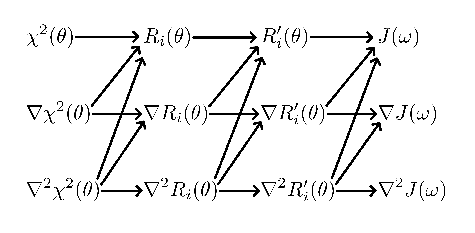
\includegraphics[width=0.8\textwidth, bb=14 14 226 110]{images/dependencies.eps.gz}}
\caption[$\chi^2$ dependencies of the values, gradients, and Hessians.]{Dependencies between the $\chi^2$, transformed relaxation, relaxation, and spectral density equations, gradients, and Hessians.}\label{fig: dependencies}
\end{figure}



% The chi-squared value, gradient, and Hessian.
%%%%%%%%%%%%%%%%%%%%%%%%%%%%%%%%%%%%%%%%%%%%%%%

\begin{latexonly}
    \section{The $\chi^2$ value, gradient, and Hessian}
\end{latexonly}
\begin{htmlonly}
    \section{The chi-squared value, gradient, and Hessian}
\end{htmlonly}

% The chi-squared value.
\begin{latexonly}
    \subsection{The $\chi^2$ value}
\end{latexonly}
\begin{htmlonly}
    \subsection{The chi-squared value}
\end{htmlonly}

The $\chi^2$ value is defined as
\begin{equation} \label{eq: maths: chi-squared}
 \chi^2(\theta) = \sum_{i=1}^n \frac{(\Ri - \Ri(\theta))^2}{\sigma_i^2},
\end{equation}

\noindent where the summation index $i$ ranges over all the relaxation data of all residues used in the analysis.



% The chi-squared gradient.
\begin{latexonly}
    \subsection{The $\chi^2$ gradient}
\end{latexonly}
\begin{htmlonly}
    \subsection{The chi-squared gradient}
\end{htmlonly}

The $\chi^2$ gradient in vector notation is
\begin{equation}
 \nabla \chi^2(\theta) = 2 \sum_{i=1}^n \frac{(\Ri - \Ri(\theta))^2}{\sigma_i^2} \nabla \Ri(\theta).
\end{equation}



% The chi-squared Hessian.
\begin{latexonly}
    \subsection{The $\chi^2$ Hessian}
\end{latexonly}
\begin{htmlonly}
    \subsection{The chi-squared Hessian}
\end{htmlonly}

The $\chi^2$ Hessian in vector notation is
\begin{equation}
 \nabla^2 \chi^2(\theta) = 2 \sum_{i=1}^n \frac{1}{\sigma_i^2} \left(\nabla \Ri(\theta) \cdot \nabla \Ri(\theta)^T - (\Ri - \Ri(\theta)) \nabla^2 \Ri(\theta) \right).
\end{equation}



% The Ri values, gradients, and Hessians.
%%%%%%%%%%%%%%%%%%%%%%%%%%%%%%%%%%%%%%%%%

\newpage
\begin{latexonly}
    \section{The $\Ri(\theta)$ values, gradients, and Hessians}
\end{latexonly}
\begin{htmlonly}
    \section{The R$_i(theta)$ values, gradients, and Hessians}
\end{htmlonly}


% The Ri values.
\begin{latexonly}
    \subsection{The $\Ri(\theta)$ values}
\end{latexonly}
\begin{htmlonly}
    \subsection{The R$_i(theta)$ values}
\end{htmlonly}

The $\Ri(\theta)$ values are given by
\begin{subequations}
\begin{align}
    \Rone(\theta) & = \Rone'(\theta), \label{eq: Ri trans: R1} \\
    \Rtwo(\theta) & = \Rtwo'(\theta), \label{eq: Ri trans: R2} \\
    \mathrm{NOE}(\theta) & = 1 + \frac{\gH}{\gX} \frac{\crossrate(\theta)}{\Rone(\theta)}. \label{eq: Ri trans: NOE}
\end{align}
\end{subequations}


% The Ri gradients.
\begin{latexonly}
    \subsection{The $\Ri(\theta)$ gradients}
\end{latexonly}
\begin{htmlonly}
    \subsection{The R$_i(theta)$ gradients}
\end{htmlonly}

The $\Ri(\theta)$ gradients in vector notation are
\begin{subequations}
\begin{align}
    \nabla \Rone(\theta) & = \nabla \Rone'(\theta), \label{eq: Ri trans: dR1} \\
    \nabla \Rtwo(\theta) & = \nabla \Rtwo'(\theta), \label{eq: Ri trans: dR2} \\
    \nabla \mathrm{NOE}(\theta) & = \frac{\gH}{\gX} \frac{1}{\Rone(\theta)^2} \Big(
        \Rone(\theta) \nabla \crossrate(\theta) - \crossrate(\theta) \nabla \Rone(\theta)
    \Big). \label{eq: Ri trans: dNOE}
\end{align}
\end{subequations}


% The Ri Hessians.
\begin{latexonly}
    \subsection{The $\Ri(\theta)$ Hessians}
\end{latexonly}
\begin{htmlonly}
    \subsection{The R$_i(theta)$ Hessians}
\end{htmlonly}

The $\Ri(\theta)$ Hessians in vector notation are
\begin{subequations}
\begin{align}
    \nabla^2 \Rone(\theta) & = \nabla^2 \Rone'(\theta), \label{eq: Ri trans: d2R1} \\
    \nabla^2 \Rtwo(\theta) & = \nabla^2 \Rtwo'(\theta), \label{eq: Ri trans: d2R2} \\
    \nabla^2 \mathrm{NOE}(\theta) & = \frac{\gH}{\gX} \frac{1}{\Rone(\theta)^3} \bigg[
        \crossrate(\theta) \Big( 2 \nabla \Rone(\theta) \cdot \nabla \Rone(\theta)^T - \Rone(\theta) \nabla^2 \Rone(\theta) \Big) \nonumber\\
        & \quad - \Rone(\theta) \Big( \nabla \crossrate(\theta) \cdot \nabla \Rone(\theta)^T - \Rone(\theta) \nabla^2 \crossrate(\theta) \Big)
    \bigg]. \label{eq: Ri trans: d2NOE}
\end{align}
\end{subequations}



% Ri' values, gradients, and Hessians.
%%%%%%%%%%%%%%%%%%%%%%%%%%%%%%%%%%%%%%

\newpage
\begin{latexonly}
    \section{$\Ri'(\theta)$ values, gradients, and Hessians}
\end{latexonly}
\begin{htmlonly}
    \section{R$_i$ $prime(theta)$ values, gradients, and Hessians}
\end{htmlonly}

The partial and second partial derivatives of the relaxation equations of the set R$'(\theta)$ are different for each parameter of the vector $\theta$.  The vector representation of the gradient $\nabla \textrm{R}_i'(\theta)$ and the matrix representation of the Hessian $\nabla^2 \textrm{R}_i'(\theta)$ can be reconstructed from the individual elements presented in the next section.


% Components.
%~~~~~~~~~~~~

\begin{latexonly}
    \subsection{Components of the $\Ri'(\theta)$ equations}
\end{latexonly}
\begin{htmlonly}
    \subsection{Components of the R$_i$ $prime(theta)$ equations}
\end{htmlonly}


To simplify the calculations of the gradients and Hessians the $\Ri'(\theta)$ equations have been broken down into a number of components.  These include the dipolar and CSA constants as well as the dipolar and CSA spectral density terms for each of the three transformed relaxation data types \{$\Rone$, $\Rtwo$, $\crossrate$\}.  The segregation of these components simplifies the maths as many partial derivatives of the components are zero.


% Dipolar comps.
\subsubsection{Dipolar constant}

The dipolar constant is defined as
\begin{equation}
    d = \frac{1}{4} \left(\frac{\mu_0}{4\pi}\right)^2 \frac{\left( \gH \gX \hbar \right)^2}{<r^6>}. \label{eq: Ri': d}
\end{equation}

\noindent This component of the relaxation equations is independent of the parameter of the spectral density function $\theta_j$, the chemical exchange parameter $\rho_{ex}$, and the CSA parameter $\Delta\sigma$.  Therefore the partial and second partial derivatives with respect to these parameters is zero.  Only the derivative with respect to the bond length $r$ is non-zero being
\begin{equation}
    d' \equiv \frac{\mathrm{d} d}{\mathrm{d} r} = - \frac{3}{2} \left(\frac{\mu_0}{4\pi}\right)^2 \frac{\left( \gH \gX \hbar \right)^2}{<r^7>}. \label{eq: Ri': d'}
\end{equation}

\noindent The second derivative with respect to the bond length is
\begin{equation}
    d'' \equiv \frac{\mathrm{d}^2 d}{\mathrm{d} r^2} = \frac{21}{2} \left(\frac{\mu_0}{4\pi}\right)^2 \frac{\left( \gH \gX \hbar \right)^2}{<r^8>}. \label{eq: Ri': d"}
\end{equation}


% CSA comps.
\subsubsection{CSA constant}

The CSA constant is defined as
\begin{equation}
    c = \frac{\left(\omega_X \cdot \Delta\sigma \right)^2}{3}. \label{eq: Ri': c}
\end{equation}

\noindent The partial derivative of this component with respect to all parameters but the CSA parameter $\Delta\sigma$ is zero.  This derivative is
\begin{equation}
    c' \equiv \frac{\mathrm{d} c}{\mathrm{d} \Delta\sigma} = \frac{2 \omega_X^2 \cdot \Delta\sigma}{3}. \label{eq: Ri': c'}
\end{equation}

\noindent The CSA constant second derivative with respect to $\Delta\sigma$ is
\begin{equation}
    c'' \equiv \frac{\mathrm{d}^2 c}{\mathrm{d} \Delta\sigma^2} = \frac{2 \omega_X^2}{3}. \label{eq: Ri': c"}
\end{equation}


% Rex comps.
\subsubsection{$R_{ex}$ constant}

The $R_{ex}$ constant is defined as
\begin{equation}
    R_{ex} = \rho_{ex} (2 \pi \omega_H)^2 . \label{eq: Ri': Rex}
\end{equation}

\noindent The partial derivative of this component with respect to all parameters but the chemical exchange parameter $\rho_{ex}$ is zero.  This derivative is
\begin{equation}
    R_{ex}' \equiv \frac{\mathrm{d} R_{ex}}{\mathrm{d} \rho_{ex}} = (2 \pi \omega_H)^2. \label{eq: Ri': Rex'}
\end{equation}

\noindent The $R_{ex}$ constant second derivative with respect to $\rho_{ex}$ is
\begin{equation}
    R_{ex}'' \equiv \frac{\mathrm{d}^2 R_{ex}}{\mathrm{d} \rho_{ex}^2} = 0. \label{eq: Ri': Rex"}
\end{equation}


% R1 dip Spectral density terms.
\subsubsection{Spectral density terms of the $\Rone$ dipolar component}

For the dipolar component of the $\Rone$ equation~\eqref{eq: R1} on page~\pageref{eq: R1} the spectral density terms are
\begin{equation}
    J_d^{\Rone} = J(\omega_H - \omega_X) + 3J(\omega_X) + 6J(\omega_H + \omega_X).  \label{eq: J terms: JR1d}
\end{equation}

\noindent The partial derivative of these terms with respect to the spectral density function parameter $\theta_j$ is
\begin{equation}
    {J_d^{\Rone}}' \equiv \frac{\partial J_d^{\Rone}}{\partial \theta_j}
        = \frac{\partial J(\omega_H - \omega_X)}{\partial \theta_j}
        + 3 \frac{\partial J(\omega_X)}{\partial \theta_j}
        + 6 \frac{\partial J(\omega_H + \omega_X)}{\partial \theta_j}.  \label{eq: J terms: JR1d'}
\end{equation}

\noindent The second partial derivative with respect to the spectral density function parameters $\theta_j$ and $\theta_k$ is
\begin{equation}
    {J_d^{\Rone}}'' \equiv \frac{\partial^2 J_d^{\Rone}}{\partial \theta_j \cdot \partial \theta_k}
        = \frac{\partial^2 J(\omega_H - \omega_X)}{\partial \theta_j \cdot \partial \theta_k}
        + 3 \frac{\partial^2 J(\omega_X)}{\partial \theta_j \cdot \partial \theta_k}
        + 6 \frac{\partial^2 J(\omega_H + \omega_X)}{\partial \theta_j \cdot \partial \theta_k}.  \label{eq: J terms: JR1d"}
\end{equation}


% R1 CSA Spectral density terms.
\subsubsection{Spectral density terms of the $\Rone$ CSA component}

For the CSA component of the $\Rone$ equation~\eqref{eq: R1} on page~\pageref{eq: R1} the spectral density terms are
\begin{equation}
    J_c^{\Rone} = J(\omega_X).  \label{eq: J terms: JR1c}
\end{equation}

\noindent The partial derivative of these terms with respect to the spectral density function parameter $\theta_j$ is
\begin{equation}
    {J_c^{\Rone}}' \equiv \frac{\partial J_c^{\Rone}}{\partial \theta_j}
        = \frac{\partial J(\omega_X)}{\partial \theta_j}.  \label{eq: J terms: JR1c'}
\end{equation}

\noindent The second partial derivative with respect to the spectral density function parameters $\theta_j$ and $\theta_k$ is
\begin{equation}
    {J_c^{\Rone}}'' \equiv \frac{\partial^2 J_c^{\Rone}}{\partial \theta_j . \partial \theta_k}
        = \frac{\partial^2 J(\omega_X)}{\partial \theta_j \cdot \partial \theta_k}.  \label{eq: J terms: JR1c"}
\end{equation}


% R2 dip Spectral density terms.
\subsubsection{Spectral density terms of the $\Rtwo$ dipolar component}

For the dipolar component of the $\Rtwo$ equation~\eqref{eq: R2} on page~\pageref{eq: R2} the spectral density terms are
\begin{equation}
    J_d^{\Rtwo} = 4J(0) + J(\omega_H - \omega_X) + 3J(\omega_X) + 6J(\omega_H) + 6J(\omega_H + \omega_X).  \label{eq: J terms: JR2d}
\end{equation}

\noindent The partial derivative of these terms with respect to the spectral density function parameter $\theta_j$ is
\begin{equation}
    {J_d^{\Rtwo}}' \equiv \frac{\partial J_d^{\Rtwo}}{\partial \theta_j}
        = 4 \frac{\partial J(0)}{\partial \theta_j}
        + \frac{\partial J(\omega_H - \omega_X)}{\partial \theta_j}
        + 3 \frac{\partial J(\omega_X)}{\partial \theta_j}
        + 6 \frac{\partial J(\omega_H)}{\partial \theta_j}
        + 6 \frac{\partial J(\omega_H + \omega_X)}{\partial \theta_j}.  \label{eq: J terms: JR2d'}
\end{equation}

\noindent The second partial derivative with respect to the spectral density function parameters $\theta_j$ and $\theta_k$ is
\begin{multline}
    {J_d^{\Rtwo}}'' \equiv \frac{\partial^2 J_d^{\Rtwo}}{\partial \theta_j \cdot \partial \theta_k}
        = 4 \frac{\partial^2 J(0)}{\partial \theta_j \cdot \partial \theta_k}
        + \frac{\partial^2 J(\omega_H - \omega_X)}{\partial \theta_j \cdot \partial \theta_k}
        + 3 \frac{\partial^2 J(\omega_X)}{\partial \theta_j \cdot \partial \theta_k} \\
        + 6 \frac{\partial^2 J(\omega_H)}{\partial \theta_j \cdot \partial \theta_k}
        + 6 \frac{\partial^2 J(\omega_H + \omega_X)}{\partial \theta_j \cdot \partial \theta_k}.  \label{eq: J terms: JR2d"}
\end{multline}


% R2 CSA Spectral density terms.
\subsubsection{Spectral density terms of the $\Rtwo$ CSA component}

For the CSA component of the $\Rtwo$ equation~\eqref{eq: R2} on page~\pageref{eq: R2} the spectral density terms are
\begin{equation}
    J_c^{\Rtwo} = 4J(0) + 3J(\omega_X).  \label{eq: J terms: JR2c}
\end{equation}

\noindent The partial derivative of these terms with respect to the spectral density function parameter $\theta_j$ is
\begin{equation}
    {J_c^{\Rtwo}}' \equiv \frac{\partial J_c^{\Rtwo}}{\partial \theta_j}
        = 4 \frac{\partial J(0)}{\partial \theta_j}
        + 3 \frac{\partial J(\omega_X)}{\partial \theta_j}.  \label{eq: J terms: JR2c'}
\end{equation}

\noindent The second partial derivative with respect to the spectral density function parameters $\theta_j$ and $\theta_k$ is
\begin{equation}
    {J_c^{\Rtwo}}'' \equiv \frac{\partial^2 J_c^{\Rtwo}}{\partial \theta_j \cdot \partial \theta_k}
        = 4 \frac{\partial^2 J(0)}{\partial \theta_j \cdot \partial \theta_k}
        + 3 \frac{\partial^2 J(\omega_X)}{\partial \theta_j \cdot \partial \theta_k}.  \label{eq: J terms: JR2c"}
\end{equation}


% Sigma_NOE dip Spectral density terms.
\begin{latexonly}
    \subsubsection{Spectral density terms of the $\crossrate$ dipolar component}
\end{latexonly}
\begin{htmlonly}
    \subsubsection{Spectral density terms of the $sigma_{NOE}$ dipolar component}
\end{htmlonly}

For the dipolar component of the $\crossrate$ equation~\eqref{eq: sigma_NOE} on page~\pageref{eq: sigma_NOE} the spectral density terms are
\begin{equation}
    J_d^{\crossrate} = 6J(\omega_H + \omega_X) - J(\omega_H - \omega_X).  \label{eq: J terms: JsigmaNOEd}
\end{equation}

\noindent The partial derivative of these terms with respect to the spectral density function parameter $\theta_j$ is
\begin{equation}
    {J_d^{\crossrate}}' \equiv \frac{\partial J_d^{\crossrate}}{\partial \theta_j}
        = 6 \frac{\partial J(\omega_H + \omega_X)}{\partial \theta_j}
          - \frac{\partial J(\omega_H - \omega_X)}{\partial \theta_j}.  \label{eq: J terms: JsigmaNOEd'}
\end{equation}

\noindent The second partial derivative with respect to the spectral density function parameters $\theta_j$ and $\theta_k$ is
\begin{equation}
    {J_d^{\crossrate}}'' \equiv \frac{\partial^2 J_d^{\crossrate}}{\partial \theta_j \cdot \partial \theta_k}
        = 6 \frac{\partial^2 J(\omega_H + \omega_X)}{\partial \theta_j \cdot \partial \theta_k}
          - \frac{\partial^2 J(\omega_H - \omega_X)}{\partial \theta_j \cdot \partial \theta_k}.  \label{eq: J terms: JsigmaNOEd"}
\end{equation}



% Ri' values.
%~~~~~~~~~~~~

\begin{latexonly}
    \subsection{$\Ri'(\theta)$ values}
\end{latexonly}
\begin{htmlonly}
    \subsection{R$_i$ $prime(theta)$ values}
\end{htmlonly}

Using the components of the relaxation equations defined above the three relaxation equations can be re-expressed as
\begin{subequations}
\begin{align}
    \Rone(\theta) & = d J_d^{\Rone} + c J_c^{\Rone},                          \label{eq: Ri': R1} \\
    \Rtwo(\theta) & = \frac{d}{2} J_d^{\Rtwo} + \frac{c}{6} J_c^{\Rtwo},      \label{eq: Ri': R2} \\
    \crossrate(\theta) & = d J_d^{\crossrate}.                          \label{eq: Ri': sigmaNOE}
\end{align}
\end{subequations}



% Ri' gradients.
%~~~~~~~~~~~~~~~

\begin{latexonly}
    \subsection{$\Ri'(\theta)$ gradients}
\end{latexonly}
\begin{htmlonly}
    \subsection{R$_i$ $prime(theta)$ gradients}
\end{htmlonly}

A different partial derivative exists for the spectral density function parameter $\theta_j$, the chemical exchange parameter $\rho_{ex}$, CSA parameter $\Delta\sigma$, and bond length parameter $r$.  In model-free analysis the spectral density parameters include both the parameters of the diffusion tensor and the parameters of the various model-free models.


% Spectral density function parameter.
\begin{latexonly}
    \subsubsection{$\theta_j$ partial derivative}
\end{latexonly}
\begin{htmlonly}
    \subsubsection{$theta_j$ partial derivative}
\end{htmlonly}

The partial derivatives of the relaxation equations with respect to the spectral density function parameter $\theta_j$ are
\begin{subequations}
\begin{align}
    \frac{\partial \Rone(\theta)}{\partial \theta_j} &= d {J_d^{\Rone}}' + c {J_c^{\Rone}}',                      \label{eq: Ri': dR1/dmf} \\
    \frac{\partial \Rtwo(\theta)}{\partial \theta_j} &= \frac{d}{2} {J_d^{\Rtwo}}' + \frac{c}{6} {J_c^{\Rtwo}}',  \label{eq: Ri': dR2/dmf} \\
    \frac{\partial \crossrate(\theta)}{\partial \theta_j} &= d {J_d^{\crossrate}}'.                         \label{eq: Ri': dsigmaNOE/dmf}
\end{align}
\end{subequations}


% Chemical exchange parameter.
\begin{latexonly}
    \subsubsection{$\rho_{ex}$ partial derivative}
\end{latexonly}
\begin{htmlonly}
    \subsubsection{$rho_{ex}$ partial derivative}
\end{htmlonly}

The partial derivatives of the relaxation equations with respect to the chemical exchange parameter $\rho_{ex}$ are
\begin{subequations}
\begin{align}
    \frac{\partial \Rone(\theta)}{\partial \rho_{ex}} &= 0,          \label{eq: Ri': dR1/dRex} \\
    \frac{\partial \Rtwo(\theta)}{\partial \rho_{ex}} &= (2 \pi \omega_H)^2,          \label{eq: Ri': dR2/dRex} \\
    \frac{\partial \crossrate(\theta)}{\partial \rho_{ex}} &= 0.   \label{eq: Ri': dsigmaNOE/dRex}
\end{align}
\end{subequations}


% CSA parameter.
\begin{latexonly}
    \subsubsection{$\Delta\sigma$ partial derivative}
\end{latexonly}
\begin{htmlonly}
    \subsubsection{$D_{sigma}$ partial derivative}
\end{htmlonly}

The partial derivatives of the relaxation equations with respect to the CSA parameter $\Delta\sigma$ are
\begin{subequations}
\begin{align}
    \frac{\partial \Rone(\theta)}{\partial \Delta\sigma} &= c' J_c^{\Rone},             \label{eq: Ri': dR1/dCSA} \\
    \frac{\partial \Rtwo(\theta)}{\partial \Delta\sigma} &= \frac{c'}{6} J_c^{\Rtwo},   \label{eq: Ri': dR2/dCSA} \\
    \frac{\partial \crossrate(\theta)}{\partial \Delta\sigma} &= 0.                 \label{eq: Ri': dsigmaNOE/dCSA}
\end{align}
\end{subequations}


% Bond length parameter.
\subsubsection{$r$ partial derivative}

The partial derivatives of the relaxation equations with respect to the bond length parameter $r$ are
\begin{subequations}
\begin{align}
    \frac{\partial \Rone(\theta)}{\partial r} &= d' J_d^{\Rone},                \label{eq: Ri': dR1/dr} \\
    \frac{\partial \Rtwo(\theta)}{\partial r} &= \frac{d'}{2} J_d^{\Rtwo},      \label{eq: Ri': dR2/dr} \\
    \frac{\partial \crossrate(\theta)}{\partial r} &= d' J_d^{\crossrate}.  \label{eq: Ri': dsigmaNOE/dr}
\end{align}
\end{subequations}



% Ri' Hessians.
%~~~~~~~~~~~~~~

\begin{latexonly}
    \subsection{$\Ri'(\theta)$ Hessians}
\end{latexonly}
\begin{htmlonly}
    \subsection{R$_i$ $prime(theta)$ Hessians}
\end{htmlonly}

Again different second partial derivatives with respect to the spectral density function parameters $\theta_j$ and $\theta_k$, the chemical exchange parameter $\rho_{ex}$, CSA parameter $\Delta\sigma$, and bond length parameter $r$.  These second partial derivatives are the components of the $\Ri'(\theta)$ Hessian matrices.


% Spectral density function parameter -- Spectral density function parameter.
\begin{latexonly}
    \subsubsection{$\theta_j$ -- $\theta_k$ partial derivative}
\end{latexonly}
\begin{htmlonly}
    \subsubsection{$theta_j$ -- $theta_k$ partial derivative}
\end{htmlonly}

The second partial derivatives of the relaxation equations with respect to the spectral density function parameters $\theta_j$ and $\theta_k$ are
\begin{subequations}
\begin{align}
    \frac{\partial^2 \Rone(\theta)}{\partial \theta_j \cdot \partial \theta_k} &= d {J_d^{\Rone}}'' + c {J_c^{\Rone}}'',                      \label{eq: Ri': d2R1/dmfj.dmfk} \\
    \frac{\partial^2 \Rtwo(\theta)}{\partial \theta_j \cdot \partial \theta_k} &= \frac{d}{2} {J_d^{\Rtwo}}'' + \frac{c}{6} {J_c^{\Rtwo}}'',  \label{eq: Ri': d2R2/dmfj.dmfk} \\
    \frac{\partial^2 \crossrate(\theta)}{\partial \theta_j \cdot \partial \theta_k} &= d {J_d^{\crossrate}}''.                          \label{eq: Ri': d2sigmaNOE/dmfj.dmfk}
\end{align}
\end{subequations}


% Spectral density function parameter -- Chemical exchange parameter.
\begin{latexonly}
    \subsubsection{$\theta_j$ -- $\rho_{ex}$ partial derivative}
\end{latexonly}
\begin{htmlonly}
    \subsubsection{$theta_j$ -- $rho_{ex}$ partial derivative}
\end{htmlonly}

The second partial derivatives of the relaxation equations with respect to the spectral density function parameter $\theta_j$ and the chemical exchange parameter $\rho_{ex}$ are
\begin{subequations}
\begin{align}
    \frac{\partial^2 \Rone(\theta)}{\partial \theta_j \cdot \partial \rho_{ex}} &= 0,        \label{eq: Ri': d2R1/dmfj.dRex} \\
    \frac{\partial^2 \Rtwo(\theta)}{\partial \theta_j \cdot \partial \rho_{ex}} &= 0,        \label{eq: Ri': d2R2/dmfj.dRex} \\
    \frac{\partial^2 \crossrate(\theta)}{\partial \theta_j \cdot \partial \rho_{ex}} &= 0. \label{eq: Ri': d2sigmaNOE/dmfj.dRex}
\end{align}
\end{subequations}


% Spectral density function parameter -- CSA parameter.
\begin{latexonly}
    \subsubsection{$\theta_j$ -- $\Delta\sigma$ partial derivative}
\end{latexonly}
\begin{htmlonly}
    \subsubsection{$theta_j$ -- $D_{sigma}$ partial derivative}
\end{htmlonly}

The second partial derivatives of the relaxation equations with respect to the spectral density function parameter $\theta_j$ and the CSA parameter $\Delta\sigma$ are
\begin{subequations}
\begin{align}
    \frac{\partial^2 \Rone(\theta)}{\partial \theta_j \cdot \partial \Delta\sigma} &= c' {J_c^{\Rone}}',            \label{eq: Ri': d2R1/dmfj.dCSA} \\
    \frac{\partial^2 \Rtwo(\theta)}{\partial \theta_j \cdot \partial \Delta\sigma} &= \frac{c'}{6} {J_c^{\Rtwo}}',  \label{eq: Ri': d2R2/dmfj.dCSA} \\
    \frac{\partial^2 \crossrate(\theta)}{\partial \theta_j \cdot \partial \Delta\sigma} &= 0.                   \label{eq: Ri': d2sigmaNOE/dmfj.dCSA}
\end{align}
\end{subequations}


% Spectral density function parameter -- Bond length parameter.
\begin{latexonly}
    \subsubsection{$\theta_j$ -- $r$ partial derivative}
\end{latexonly}
\begin{htmlonly}
    \subsubsection{$theta_j$ -- $r$ partial derivative}
\end{htmlonly}

The second partial derivatives of the relaxation equations with respect to the spectral density function parameter $\theta_j$ and the bond length parameter $r$ are
\begin{subequations}
\begin{align}
    \frac{\partial^2 \Rone(\theta)}{\partial \theta_j \cdot \partial r} &= d' {J_d^{\Rone}}',               \label{eq: Ri': d2R1/dmfj.dr} \\
    \frac{\partial^2 \Rtwo(\theta)}{\partial \theta_j \cdot \partial r} &= \frac{d'}{2} {J_d^{\Rtwo}}',     \label{eq: Ri': d2R2/dmfj.dr} \\
    \frac{\partial^2 \crossrate(\theta)}{\partial \theta_j \cdot \partial r} &= d' {J_d^{\crossrate}}'. \label{eq: Ri': d2sigmaNOE/dmfj.dr}
\end{align}
\end{subequations}


% Chemical exchange parameter -- Chemical exchange parameter.
\begin{latexonly}
    \subsubsection{$\rho_{ex}$ -- $\rho_{ex}$ partial derivative}
\end{latexonly}
\begin{htmlonly}
    \subsubsection{$rho_{ex}$ -- $rho_{ex}$ partial derivative}
\end{htmlonly}

The second partial derivatives of the relaxation equations with respect to the chemical exchange parameter $\rho_{ex}$ twice are
\begin{subequations}
\begin{align}
    \frac{\partial^2 \Rone(\theta)}{{\partial \rho_{ex}}^2} &= 0,        \label{eq: Ri': d2R1/dRex2} \\
    \frac{\partial^2 \Rtwo(\theta)}{{\partial \rho_{ex}}^2} &= 0,        \label{eq: Ri': d2R2/dRex2} \\
    \frac{\partial^2 \crossrate(\theta)}{{\partial \rho_{ex}}^2} &= 0. \label{eq: Ri': d2sigmaNOE/dRex2}
\end{align}
\end{subequations}


% Chemical exchange parameter -- CSA parameter.
\begin{latexonly}
    \subsubsection{$\rho_{ex}$ -- $\Delta\sigma$ partial derivative}
\end{latexonly}
\begin{htmlonly}
    \subsubsection{$rho_{ex}$ -- $D_{sigma}$ partial derivative}
\end{htmlonly}

The second partial derivatives of the relaxation equations with respect to the chemical exchange parameter $\rho_{ex}$ and the CSA parameter $\Delta\sigma$ are
\begin{subequations}
\begin{align}
    \frac{\partial^2 \Rone(\theta)}{\partial \rho_{ex} \cdot \partial \Delta\sigma} &= 0,        \label{eq: Ri': d2R1/dRex.dCSA} \\
    \frac{\partial^2 \Rtwo(\theta)}{\partial \rho_{ex} \cdot \partial \Delta\sigma} &= 0,        \label{eq: Ri': d2R2/dRex.dCSA} \\
    \frac{\partial^2 \crossrate(\theta)}{\partial \rho_{ex} \cdot \partial \Delta\sigma} &= 0. \label{eq: Ri': d2sigmaNOE/dRex.dCSA}
\end{align}
\end{subequations}


% Chemical exchange parameter -- Bond length parameter.
\begin{latexonly}
    \subsubsection{$\rho_{ex}$ -- $r$ partial derivative}
\end{latexonly}
\begin{htmlonly}
    \subsubsection{$rho_{ex}$ -- $r$ partial derivative}
\end{htmlonly}

The second partial derivatives of the relaxation equations with respect to the chemical exchange parameter $\rho_{ex}$ and the bond length parameter $r$ are
\begin{subequations}
\begin{align}
    \frac{\partial^2 \Rone(\theta)}{\partial \rho_{ex} \cdot \partial r} &= 0,           \label{eq: Ri': d2R1/dRex.dr} \\
    \frac{\partial^2 \Rtwo(\theta)}{\partial \rho_{ex} \cdot \partial r} &= 0,           \label{eq: Ri': d2R2/dRex.dr} \\
    \frac{\partial^2 \crossrate(\theta)}{\partial \rho_{ex} \cdot \partial r} &= 0.    \label{eq: Ri': d2sigmaNOE/dRex.dr}
\end{align}
\end{subequations}


% CSA parameter -- CSA parameter.
\begin{latexonly}
    \subsubsection{$\Delta\sigma$ -- $\Delta\sigma$ partial derivative}
\end{latexonly}
\begin{htmlonly}
    \subsubsection{$D_{sigma}$ -- $D_{sigma}$ partial derivative}
\end{htmlonly}

The second partial derivatives of the relaxation equations with respect to the CSA parameter $\Delta\sigma$ twice are
\begin{subequations}
\begin{align}
    \frac{\partial^2 \Rone(\theta)}{{\partial \Delta\sigma}^2} &= c'' J_c^{\Rone},              \label{eq: Ri': d2R1/dCSA2} \\
    \frac{\partial^2 \Rtwo(\theta)}{{\partial \Delta\sigma}^2} &= \frac{c''}{6} J_c^{\Rtwo},    \label{eq: Ri': d2R2/dCSA2} \\
    \frac{\partial^2 \crossrate(\theta)}{{\partial \Delta\sigma}^2} &= 0.                   \label{eq: Ri': d2sigmaNOE/dCSA2}
\end{align}
\end{subequations}


% CSA parameter -- Bond length parameter.
\begin{latexonly}
    \subsubsection{$\Delta\sigma$ -- $r$ partial derivative}
\end{latexonly}
\begin{htmlonly}
    \subsubsection{$D_{sigma}$ -- $r$ partial derivative}
\end{htmlonly}

The second partial derivatives of the relaxation equations with respect to the CSA parameter $\Delta\sigma$ and the bond length parameter $r$ are
\begin{subequations}
\begin{align}
    \frac{\partial^2 \Rone(\theta)}{\partial \Delta\sigma \cdot \partial r} &= 0,         \label{eq: Ri': d2R1/dCSA.dr} \\
    \frac{\partial^2 \Rtwo(\theta)}{\partial \Delta\sigma \cdot \partial r} &= 0,         \label{eq: Ri': d2R2/dCSA.dr} \\
    \frac{\partial^2 \crossrate(\theta)}{\partial \Delta\sigma \cdot \partial r} &= 0.  \label{eq: Ri': d2sigmaNOE/dCSA.dr}
\end{align}
\end{subequations}


% Bond length parameter -- Bond length parameter.
\subsubsection{$r$ -- $r$ partial derivative}

The second partial derivatives of the relaxation equations with respect to the bond length parameter $r$ twice are
\begin{subequations}
\begin{align}
    \frac{\partial^2 \Rone(\theta)}{{\partial r}^2} &= d'' J_d^{\Rone},                 \label{eq: Ri': d2R1/dr2} \\
    \frac{\partial^2 \Rtwo(\theta)}{{\partial r}^2} &= \frac{d''}{2} J_d^{\Rtwo},       \label{eq: Ri': d2R2/dr2} \\
    \frac{\partial^2 \crossrate(\theta)}{{\partial r}^2} &= d'' J_d^{\crossrate}.   \label{eq: Ri': d2sigmaNOE/dr2}
\end{align}
\end{subequations}




% Model-free analysis.
%%%%%%%%%%%%%%%%%%%%%%

\newpage
\section{Model-free analysis}



% The model-free equations.
%~~~~~~~~~~~~~~~~~~~~~~~~~~

\subsection{The model-free equations}

In the original model-free analysis of \cite{LipariSzabo82a} the correlation function $C(\tau)$ of the XH bond vector is approximated by decoupling the internal fluctuations of the bond vector $C_\mathrm{I}(\tau)$ from the correlation function of the overall Brownian rotational diffusion $C_\mathrm{O}(\tau)$ by the equation
\begin{equation}
    C(\tau) = C_\mathrm{O}(\tau) \cdot C_\mathrm{I}(\tau).
\end{equation}

\noindent The overall correlation functions of the diffusion of a sphere, spheroid, and ellipsoid are presented respectively in section~\ref{ellipsoid equation} on page~\pageref{ellipsoid equation}, section~\ref{spheroid equation} on page~\pageref{spheroid equation}, and section~\ref{sphere equation} on page~\pageref{sphere equation}.  These three different equations can be combined into one generic correlation function which is independent of the type of diffusion.  This generic correlation function is
\begin{equation}
    C_\mathrm{O}(\tau) = \frac{1}{5} \sum_{i=-k}^k c_i \cdot e^{-\tau/\tau_i},
\end{equation}

\noindent where $c_i$ are the weights and $\tau_i$ are correlation times of the exponential terms.  In the original model-free analysis of \citet{LipariSzabo82a,LipariSzabo82b} the internal motions are modelled by the correlation function
\begin{equation}
    C_\mathrm{I}(\tau) = S^2 + (1 - S^2) e^{-\tau / \tau_e},
\end{equation}

\noindent where $S^2$ is the generalised Lipari and Szabo order parameter which is related to the amplitude of the motion and $\tau_e$ is the effective correlation time which is an indicator of the timescale of the motion, albeit being dependent on the value of the order parameter.  The order parameter ranges from one for complete rigidity to zero for unrestricted motions.  Model-free theory was extended by \citet{Clore90a} to include motions on two timescales by the correlation function
\begin{equation}
    C_\mathrm{I}(\tau) = S^2 + (1 - S^2_f) e^{-\tau / \tau_f} + (S^2_f - S^2) e^{-\tau / \tau_s},
\end{equation}

\noindent where the faster of the motions is defined by the order parameter $S^2_f$ and the correlation time $\tau_f$, the slower by the parameters $S^2_s$ and $\tau_s$, and the two order parameter are related by the equation $S^2 = S^2_f \cdot S^2_s$.

The relaxation equations of \citet{Abragam61} are composed of a sum of power spectral density functions $J(\omega)$ at five frequencies.  The spectral density function is related to the correlation function as the two are a Fourier pair.  Applying the Fourier transform to the correlation function composed of the generic diffusion equation and the original model-free correlation function results in the equation
\begin{equation} \label{eq: maths: J(w) model-free generic}
    J(\omega) = \frac{2}{5} \sum_{i=-k}^k c_i \cdot \tau_i \Bigg(
        \frac{S^2}{1 + (\omega \tau_i)^2}
        + \frac{(1 - S^2)(\tau_e + \tau_i)\tau_e}{(\tau_e + \tau_i)^2 + (\omega \tau_e \tau_i)^2}
    \Bigg).
\end{equation}

The Fourier transform using the extended model-free correlation function is
\begin{equation} \label{eq: maths: J(w) model-free ext generic}
    J(\omega) = \frac{2}{5} \sum_{i=-k}^k c_i \cdot \tau_i \Bigg(
        \frac{S^2}{1 + (\omega \tau_i)^2}
        + \frac{(1 - S^2_f)(\tau_f + \tau_i)\tau_f}{(\tau_f + \tau_i)^2 + (\omega \tau_f \tau_i)^2}
        + \frac{(S^2_f - S^2)(\tau_s + \tau_i)\tau_s}{(\tau_s + \tau_i)^2 + (\omega \tau_s \tau_i)^2}
    \Bigg).
\end{equation}



% The original model-free gradient.
%~~~~~~~~~~~~~~~~~~~~~~~~~~~~~~~~~~

\subsection{The original model-free gradient}

The model-free gradient of the original spectral density function~\eqref{eq: maths: J(w) model-free generic} is the vector of partial derivatives of the function with respect to the geometric parameter $\Diffgeoset_i$, the orientational parameter $\Difforiset_i$, the order parameter $S^2$, and the internal correlation time $\tau_e$.  The positions in the vector correspond to the model parameters which are being optimised.



% Gj partial derivative.
\begin{latexonly}
    \subsubsection{$\Diffgeoset_j$ partial derivative}
\end{latexonly}
\begin{htmlonly}
    \subsubsection{$S_j$ partial derivative}
\end{htmlonly}

The partial derivative of~\eqref{eq: maths: J(w) model-free generic} with respect to the geometric parameter $\Diffgeoset_j$ is
\begin{multline}
    \frac{\partial J(\omega)}{\partial \Diffgeoset_j} = \frac{2}{5} \sum_{i=-k}^k \Bigg(
        c_i \frac{\partial \tau_i}{\partial \Diffgeoset_j} \Bigg(
            S^2 \frac{1 - (\omega \tau_i)^2}{\left(1 + (\omega \tau_i)^2 \right)^2}
            + (1 - S^2) \tau_e^2 \frac{(\tau_e + \tau_i)^2 - (\omega \tau_e \tau_i)^2}{\left((\tau_e + \tau_i)^2 + (\omega \tau_e \tau_i)^2 \right)^2}
        \Bigg) \\
        +  \frac{\partial c_i}{\partial \Diffgeoset_j} \tau_i \Bigg(
            \frac{S^2}{1 + (\omega \tau_i)^2}
            + \frac{(1 - S^2)(\tau_e + \tau_i)\tau_e}{(\tau_e + \tau_i)^2 + (\omega \tau_e \tau_i)^2}
        \Bigg)
    \Bigg).
\end{multline}



% Oj partial derivative.
\begin{latexonly}
    \subsubsection{$\Difforiset_j$ partial derivative}
\end{latexonly}
\begin{htmlonly}
    \subsubsection{$O_j$ partial derivative}
\end{htmlonly}

The partial derivative of~\eqref{eq: maths: J(w) model-free generic} with respect to the orientational parameter $\Difforiset_j$ is
\begin{equation}
    \frac{\partial J(\omega)}{\partial \Difforiset_j} = \frac{2}{5} \sum_{i=-k}^k \frac{\partial c_i}{\partial \Difforiset_j} \tau_i \Bigg(
        \frac{S^2}{1 + (\omega \tau_i)^2}
        + \frac{(1 - S^2)(\tau_e + \tau_i)\tau_e}{(\tau_e + \tau_i)^2 + (\omega \tau_e \tau_i)^2}
    \Bigg).
\end{equation}



% S2 partial derivative.
\subsubsection{$S^2$ partial derivative}

The partial derivative of~\eqref{eq: maths: J(w) model-free generic} with respect to the order parameter $S^2$ is
\begin{equation}
    \frac{\partial J(\omega)}{\partial S^2} = \frac{2}{5} \sum_{i=-k}^k c_i \tau_i \Bigg(
        \frac{1}{1 + (\omega \tau_i)^2}
        - \frac{(\tau_e + \tau_i)\tau_e}{(\tau_e + \tau_i)^2 + (\omega \tau_e \tau_i)^2}
    \Bigg).
\end{equation}



% te partial derivative.
\begin{latexonly}
    \subsubsection{$\tau_e$ partial derivative}
\end{latexonly}
\begin{htmlonly}
    \subsubsection{$tau_e$ partial derivative}
\end{htmlonly}

The partial derivative of~\eqref{eq: maths: J(w) model-free generic} with respect to the correlation time $\tau_e$ is
\begin{equation}
    \frac{\partial J(\omega)}{\partial \tau_e} = \frac{2}{5} (1 - S^2) \sum_{i=-k}^k c_i \tau_i^2
        \frac{(\tau_e + \tau_i)^2 - (\omega \tau_e \tau_i)^2}{\left((\tau_e + \tau_i)^2 + (\omega \tau_e \tau_i)^2 \right)^2}.
\end{equation}



% The original model-free Hessian.
%~~~~~~~~~~~~~~~~~~~~~~~~~~~~~~~~~

\newpage
\subsection{The original model-free Hessian}

The model-free Hessian of the original spectral density function~\eqref{eq: maths: J(w) model-free generic} is the matrix of second partial derivatives.  The matrix coordinates correspond to the model parameters which are being optimised.



% Gj-Gk partial derivative.
\begin{latexonly}
    \subsubsection{$\Diffgeoset_j$ -- $\Diffgeoset_k$ partial derivative}
\end{latexonly}
\begin{htmlonly}
    \subsubsection{$G_j$ -- $G_k$ partial derivative}
\end{htmlonly}

The second partial derivative of~\eqref{eq: maths: J(w) model-free generic} with respect to the geometric parameters $\Diffgeoset_j$ and $\Diffgeoset_k$ is
\begin{multline}
    \frac{\partial^2 J(\omega)}{\partial \Diffgeoset_j \cdot \partial \Diffgeoset_k} = \frac{2}{5} \sum_{i=-k}^k \Bigg(
        -2 c_i \frac{\partial \tau_i}{\partial \Diffgeoset_j} \cdot \frac{\partial \tau_i}{\partial \Diffgeoset_k} \Bigg(
            S^2 \omega^2 \tau_i \frac{3 - (\omega \tau_i)^2}{\left(1 + (\omega \tau_i)^2 \right)^3}  \\
            + (1 - S^2) \tau_e^2 \frac{(\tau_e + \tau_i)^3  +  3 \omega^2 \tau_e^3 \tau_i (\tau_e + \tau_i)  -  (\omega \tau_e)^4 \tau_i^3}
                {\left((\tau_e + \tau_i)^2 + (\omega \tau_e \tau_i)^2 \right)^3}
        \Bigg) \\
        + \Bigg(
            \frac{\partial \tau_i}{\partial \Diffgeoset_j} \cdot \frac{\partial c_i}{\partial \Diffgeoset_k}
            + \frac{\partial \tau_i}{\partial \Diffgeoset_k} \cdot \frac{\partial c_i}{\partial \Diffgeoset_j}
            + c_i \frac{\partial^2 \tau_i}{\partial \Diffgeoset_j \cdot \partial \Diffgeoset_k}
        \Bigg)
        \Bigg(
            S^2 \frac{1 - (\omega \tau_i)^2}{\left(1 + (\omega \tau_i)^2 \right)^2} \\
            + (1 - S^2) \tau_e^2 \frac{(\tau_e + \tau_i)^2 - (\omega \tau_e \tau_i)^2}{\left((\tau_e + \tau_i)^2 + (\omega \tau_e \tau_i)^2 \right)^2}
        \Bigg) \\
        + \Bigg(
            \frac{\partial^2 c_i}{\partial \Diffgeoset_j \cdot \partial \Diffgeoset_k} \tau_i \Bigg(
                \frac{S^2}{1 + (\omega \tau_i)^2}
                + \frac{(1 - S^2)(\tau_e + \tau_i)\tau_e}{(\tau_e + \tau_i)^2 + (\omega \tau_e \tau_i)^2}
            \Bigg)
        \Bigg)
    \Bigg).
\end{multline}
                


% Gj-Ok partial derivative.
\begin{latexonly}
    \subsubsection{$\Diffgeoset_j$ -- $\Difforiset_k$ partial derivative}
\end{latexonly}
\begin{htmlonly}
    \subsubsection{$G_j$ -- $O_k$ partial derivative}
\end{htmlonly}

The second partial derivative of~\eqref{eq: maths: J(w) model-free generic} with respect to the geometric parameter $\Diffgeoset_j$ and the orientational parameter $\Difforiset_k$ is
\begin{multline}
    \frac{\partial^2 J(\omega)}{\partial \Diffgeoset_j \cdot \partial \Difforiset_k} = \frac{2}{5} \sum_{i=-k}^k \Bigg(
        \frac{\partial \tau_i}{\partial \Diffgeoset_j} \frac{\partial c_i}{\partial \Difforiset_k} \Bigg(
            S^2 \frac{1 - (\omega \tau_i)^2}{\left(1 + (\omega \tau_i)^2 \right)^2}
            + (1 - S^2) \tau_e^2 \frac{(\tau_e + \tau_i)^2 - (\omega \tau_e \tau_i)^2}{\left((\tau_e + \tau_i)^2 + (\omega \tau_e \tau_i)^2 \right)^2}
        \Bigg) \\
        +  \frac{\partial^2 c_i}{\partial \Diffgeoset_j \cdot \partial \Difforiset_k} \tau_i \Bigg(
            \frac{S^2}{1 + (\omega \tau_i)^2}
            + \frac{(1 - S^2)(\tau_e + \tau_i)\tau_e}{(\tau_e + \tau_i)^2 + (\omega \tau_e \tau_i)^2}
        \Bigg)
    \Bigg).
\end{multline}



% Gj-S2 partial derivative.
\begin{latexonly}
    \subsubsection{$\Diffgeoset_j$ -- $S^2$ partial derivative}
\end{latexonly}
\begin{htmlonly}
    \subsubsection{$G_j$ -- $S^2$ partial derivative}
\end{htmlonly}

The second partial derivative of~\eqref{eq: maths: J(w) model-free generic} with respect to the geometric parameter $\Diffgeoset_j$ and the order parameter $S^2$ is
\begin{multline}
    \frac{\partial^2 J(\omega)}{\partial \Diffgeoset_j \cdot \partial S^2} = \frac{2}{5} \sum_{i=-k}^k \Bigg(
        c_i \frac{\partial \tau_i}{\partial \Diffgeoset_j} \Bigg(
            \frac{1 - (\omega \tau_i)^2}{\left(1 + (\omega \tau_i)^2 \right)^2}
            - \tau_e^2 \frac{(\tau_e + \tau_i)^2 - (\omega \tau_e \tau_i)^2}{\left((\tau_e + \tau_i)^2 + (\omega \tau_e \tau_i)^2 \right)^2}
        \Bigg) \\
        +  \frac{\partial c_i}{\partial \Diffgeoset_j} \tau_i \Bigg(
            \frac{1}{1 + (\omega \tau_i)^2}
            - \frac{(\tau_e + \tau_i)\tau_e}{(\tau_e + \tau_i)^2 + (\omega \tau_e \tau_i)^2}
        \Bigg)
    \Bigg).
\end{multline}



% Gj-te partial derivative.
\begin{latexonly}
    \subsubsection{$\Diffgeoset_j$ -- $\tau_e$ partial derivative}
\end{latexonly}
\begin{htmlonly}
    \subsubsection{$G_j$ -- $tau_e$ partial derivative}
\end{htmlonly}

The second partial derivative of~\eqref{eq: maths: J(w) model-free generic} with respect to the geometric parameter $\Diffgeoset_j$ and the correlation time $\tau_e$ is
\begin{multline}
    \frac{\partial^2 J(\omega)}{\partial \Diffgeoset_j \cdot \partial \tau_e} = \frac{2}{5} (1 - S^2) \sum_{i=-k}^k \Bigg(
        2 c_i \frac{\partial \tau_i}{\partial \Diffgeoset_j} \tau_e \tau_i (\tau_e + \tau_i)
            \frac{(\tau_e + \tau_i)^2 - 3(\omega \tau_e \tau_i)^2}{\left((\tau_e + \tau_i)^2 + (\omega \tau_e \tau_i)^2 \right)^3}  \\
        + \frac{\partial c_i}{\partial \Diffgeoset_j} \tau_i^2 \frac{(\tau_e + \tau_i)^2 - (\omega \tau_e \tau_i)^2}{\left((\tau_e + \tau_i)^2 + (\omega \tau_e \tau_i)^2 \right)^2}
    \Bigg).
\end{multline}


% Oj-Ok partial derivative.
\begin{latexonly}
    \subsubsection{$\Difforiset_j$ -- $\Difforiset_k$ partial derivative}
\end{latexonly}
\begin{htmlonly}
    \subsubsection{$O_j$ -- $O_k$ partial derivative}
\end{htmlonly}

The second partial derivative of~\eqref{eq: maths: J(w) model-free generic} with respect to the orientational parameters $\Difforiset_j$ and $\Difforiset_k$ is
\begin{equation}
    \frac{\partial^2 J(\omega)}{\partial \Difforiset_j \cdot \partial \Difforiset_k} = \frac{2}{5} \sum_{i=-k}^k
        \frac{\partial^2 c_i}{\partial \Difforiset_j \cdot \partial \Difforiset_k} \tau_i \Bigg(
            \frac{S^2}{1 + (\omega \tau_i)^2}
            + \frac{(1 - S^2)(\tau_e + \tau_i)\tau_e}{(\tau_e + \tau_i)^2 + (\omega \tau_e \tau_i)^2}
        \Bigg).
\end{equation}



% Oj-S2 partial derivative.
\begin{latexonly}
    \subsubsection{$\Difforiset_j$ -- $S^2$ partial derivative}
\end{latexonly}
\begin{htmlonly}
    \subsubsection{$O_j$ -- $S^2$ partial derivative}
\end{htmlonly}

The second partial derivative of~\eqref{eq: maths: J(w) model-free generic} with respect to the orientational parameter $\Difforiset_j$ and the order parameter $S^2$ is
\begin{equation}
    \frac{\partial^2 J(\omega)}{\partial \Difforiset_j \cdot \partial S^2} = \frac{2}{5} \sum_{i=-k}^k \frac{\partial c_i}{\partial \Difforiset_j} \tau_i \Bigg(
        \frac{1}{1 + (\omega \tau_i)^2}
        - \frac{(\tau_e + \tau_i)\tau_e}{(\tau_e + \tau_i)^2 + (\omega \tau_e \tau_i)^2}
    \Bigg).
\end{equation}



% Oj-te partial derivative.
\begin{latexonly}
    \subsubsection{$\Difforiset_j$ -- $\tau_e$ partial derivative}
\end{latexonly}
\begin{htmlonly}
    \subsubsection{$O_j$ -- $tau_e$ partial derivative}
\end{htmlonly}

The second partial derivative of~\eqref{eq: maths: J(w) model-free generic} with respect to the orientational parameter $\Difforiset_j$ and the correlation time $\tau_e$ is
\begin{equation}
    \frac{\partial^2 J(\omega)}{\partial \Difforiset_j \cdot \partial \tau_e} = \frac{2}{5} (1 - S^2) \sum_{i=-k}^k
        \frac{\partial c_i}{\partial \Difforiset_j} \tau_i^2
        \frac{(\tau_e + \tau_i)^2 - (\omega \tau_e \tau_i)^2}{\left((\tau_e + \tau_i)^2 + (\omega \tau_e \tau_i)^2 \right)^2}.
\end{equation}



% S2-S2 partial derivative.
\subsubsection{$S^2$ -- $S^2$ partial derivative}

The second partial derivative of~\eqref{eq: maths: J(w) model-free generic} with respect to the order parameter $S^2$ twice is
\begin{equation}
    \frac{\partial^2 J(\omega)}{(\partial S^2)^2} = 0.
\end{equation}



% S2-te partial derivative.
\begin{latexonly}
    \subsubsection{$S^2$ -- $\tau_e$ partial derivative}
\end{latexonly}
\begin{htmlonly}
    \subsubsection{$S^2$ -- $tau_e$ partial derivative}
\end{htmlonly}

The second partial derivative of~\eqref{eq: maths: J(w) model-free generic} with respect to the order parameter $S^2$ and correlation time $\tau_e$ is
\begin{equation}
    \frac{\partial^2 J(\omega)}{\partial S^2 \cdot \partial \tau_e} = -\frac{2}{5} \sum_{i=-k}^k c_i \tau_i^2
        \frac{(\tau_e + \tau_i)^2 - (\omega \tau_e \tau_i)^2}{\left((\tau_e + \tau_i)^2 + (\omega \tau_e \tau_i)^2 \right)^2}.
\end{equation}



% te-te partial derivative.
\begin{latexonly}
    \subsubsection{$\tau_e$ -- $\tau_e$ partial derivative}
\end{latexonly}
\begin{htmlonly}
    \subsubsection{$tau_e$ -- $tau_e$ partial derivative}
\end{htmlonly}

The second partial derivative of~\eqref{eq: maths: J(w) model-free generic} with respect to the correlation time $\tau_e$ twice is
\begin{equation}
    \frac{\partial^2 J(\omega)}{{\partial \tau_e}^2} = -\frac{4}{5} (1 - S^2) \sum_{i=-k}^k c_i \tau_i^2
        \frac{(\tau_e + \tau_i)^3  +  3 \omega^2 \tau_i^3 \tau_e (\tau_e + \tau_i)  -  (\omega \tau_i)^4 \tau_e^3}
            {\left((\tau_e + \tau_i)^2 + (\omega \tau_e \tau_i)^2 \right)^3}
\end{equation}




% The extended model-free gradient.
%~~~~~~~~~~~~~~~~~~~~~~~~~~~~~~~~~~

\newpage
\subsection{The extended model-free gradient}

The model-free gradient of the extended spectral density function~\eqref{eq: maths: J(w) model-free ext generic} is the vector of partial derivatives of the function with respect to the geometric parameter $\Diffgeoset_i$, the orientational parameter $\Difforiset_i$, the order parameters $S^2$ and $S^2_f$, and the internal correlation times $\tau_f$ and $\tau_s$.  The positions in the vector correspond to the model parameters which are being optimised.



% Gj partial derivative.
\begin{latexonly}
    \subsubsection{$\Diffgeoset_j$ partial derivative}
\end{latexonly}
\begin{htmlonly}
    \subsubsection{$G_j$ partial derivative}
\end{htmlonly}

The partial derivative of~\eqref{eq: maths: J(w) model-free ext generic} with respect to the geometric parameter $\Diffgeoset_j$ is
\begin{multline}
    \frac{\partial J(\omega)}{\partial \Diffgeoset_j} = \frac{2}{5} \sum_{i=-k}^k \Bigg(
        c_i \frac{\partial \tau_i}{\partial \Diffgeoset_j} \Bigg(
            S^2 \frac{1 - (\omega \tau_i)^2}{\left(1 + (\omega \tau_i)^2 \right)^2} \\
            + (1 - S^2_f) \tau_f^2 \frac{(\tau_f + \tau_i)^2 - (\omega \tau_f \tau_i)^2}{\left((\tau_f + \tau_i)^2 + (\omega \tau_f \tau_i)^2 \right)^2} \\
            + (S^2_f - S^2) \tau_s^2 \frac{(\tau_s + \tau_i)^2 - (\omega \tau_s \tau_i)^2}{\left((\tau_s + \tau_i)^2 + (\omega \tau_s \tau_i)^2 \right)^2}
        \Bigg) \\
        +  \frac{\partial c_i}{\partial \Diffgeoset_j} \tau_i \Bigg(
            \frac{S^2}{1 + (\omega \tau_i)^2}
            + \frac{(1 - S^2_f)(\tau_f + \tau_i)\tau_f}{(\tau_f + \tau_i)^2 + (\omega \tau_f \tau_i)^2}
            + \frac{(S^2_f - S^2)(\tau_s + \tau_i)\tau_s}{(\tau_s + \tau_i)^2 + (\omega \tau_s \tau_i)^2}
        \Bigg)
    \Bigg).
\end{multline}



% Oj partial derivative.
\begin{latexonly}
    \subsubsection{$\Difforiset_j$ partial derivative}
\end{latexonly}
\begin{htmlonly}
    \subsubsection{$O_j$ partial derivative}
\end{htmlonly}

The partial derivative of~\eqref{eq: maths: J(w) model-free ext generic} with respect to the orientational parameter $\Difforiset_j$ is
\begin{equation}
    \frac{\partial J(\omega)}{\partial \Difforiset_j} = \frac{2}{5} \sum_{i=-k}^k \frac{\partial c_i}{\partial \Difforiset_j} \tau_i \Bigg(
        \frac{S^2}{1 + (\omega \tau_i)^2}
        + \frac{(1 - S^2_f)(\tau_f + \tau_i)\tau_f}{(\tau_f + \tau_i)^2 + (\omega \tau_f \tau_i)^2}
        + \frac{(S^2_f - S^2)(\tau_s + \tau_i)\tau_s}{(\tau_s + \tau_i)^2 + (\omega \tau_s \tau_i)^2}
    \Bigg).
\end{equation}



% S2 partial derivative.
\subsubsection{$S^2$ partial derivative}

The partial derivative of~\eqref{eq: maths: J(w) model-free ext generic} with respect to the order parameter $S^2$ is
\begin{equation}
    \frac{\partial J(\omega)}{\partial S^2} = \frac{2}{5} \sum_{i=-k}^k c_i \tau_i \Bigg(
        \frac{1}{1 + (\omega \tau_i)^2}
        - \frac{(\tau_s + \tau_i)\tau_s}{(\tau_s + \tau_i)^2 + (\omega \tau_s \tau_i)^2}
    \Bigg).
\end{equation}



% S2f partial derivative.
\subsubsection{$S^2_f$ partial derivative}

The partial derivative of~\eqref{eq: maths: J(w) model-free ext generic} with respect to the order parameter $S^2_f$ is
\begin{equation}
    \frac{\partial J(\omega)}{\partial S^2_f} = -\frac{2}{5} \sum_{i=-k}^k c_i \tau_i \Bigg(
        \frac{(\tau_f + \tau_i)\tau_f}{(\tau_f + \tau_i)^2 + (\omega \tau_f \tau_i)^2}
        - \frac{(\tau_s + \tau_i)\tau_s}{(\tau_s + \tau_i)^2 + (\omega \tau_s \tau_i)^2}
    \Bigg).
\end{equation}



% tf partial derivative.
\begin{latexonly}
    \subsubsection{$\tau_f$ partial derivative}
\end{latexonly}
\begin{htmlonly}
    \subsubsection{$tau_f$ partial derivative}
\end{htmlonly}

The partial derivative of~\eqref{eq: maths: J(w) model-free ext generic} with respect to the correlation time $\tau_f$ is
\begin{equation}
    \frac{\partial J(\omega)}{\partial \tau_f} = \frac{2}{5} (1 - S^2_f) \sum_{i=-k}^k c_i \tau_i^2
        \frac{(\tau_f + \tau_i)^2 - (\omega \tau_f \tau_i)^2}{\left((\tau_f + \tau_i)^2 + (\omega \tau_f \tau_i)^2 \right)^2}.
\end{equation}



% ts partial derivative.
\begin{latexonly}
    \subsubsection{$\tau_s$ partial derivative}
\end{latexonly}
\begin{htmlonly}
    \subsubsection{$tau_s$ partial derivative}
\end{htmlonly}

The partial derivative of~\eqref{eq: maths: J(w) model-free ext generic} with respect to the correlation time $\tau_s$ is
\begin{equation}
    \frac{\partial J(\omega)}{\partial \tau_s} = \frac{2}{5} (S^2_f - S^2) \sum_{i=-k}^k c_i \tau_i^2
        \frac{(\tau_s + \tau_i)^2 - (\omega \tau_s \tau_i)^2}{\left((\tau_s + \tau_i)^2 + (\omega \tau_s \tau_i)^2 \right)^2}.
\end{equation}




% The extended model-free Hessian.
%~~~~~~~~~~~~~~~~~~~~~~~~~~~~~~~~~

\newpage
\subsection{The extended model-free Hessian}

The model-free Hessian of the extended spectral density function~\eqref{eq: maths: J(w) model-free ext generic} is the matrix of second partial derivatives.  The matrix coordinates correspond to the model parameters which are being optimised.



% Gj-Gk partial derivative.
\begin{latexonly}
    \subsubsection{$\Diffgeoset_j$ -- $\Diffgeoset_k$ partial derivative}
\end{latexonly}
\begin{htmlonly}
    \subsubsection{$G_j$ -- $G_k$ partial derivative}
\end{htmlonly}

The second partial derivative of~\eqref{eq: maths: J(w) model-free ext generic} with respect to the geometric parameters $\Diffgeoset_j$ and $\Diffgeoset_k$ is
\begin{multline}
    \frac{\partial^2 J(\omega)}{\partial \Diffgeoset_j \cdot \partial \Diffgeoset_k} = \frac{2}{5} \sum_{i=-k}^k \Bigg(
        -2 c_i \frac{\partial \tau_i}{\partial \Diffgeoset_j} \cdot \frac{\partial \tau_i}{\partial \Diffgeoset_k} \Bigg(
            S^2 \omega^2 \tau_i \frac{3 - (\omega \tau_i)^2}{\left(1 + (\omega \tau_i)^2 \right)^3}  \\
            + (1 - S^2_f) \tau_f^2 \frac{(\tau_f + \tau_i)^3  +  3 \omega^2 \tau_f^3 \tau_i (\tau_f + \tau_i)  -  (\omega \tau_f)^4 \tau_i^3}
                {\left((\tau_f + \tau_i)^2 + (\omega \tau_f \tau_i)^2 \right)^3} \\
            + (S^2_f - S^2) \tau_s^2 \frac{(\tau_s + \tau_i)^3  +  3 \omega^2 \tau_s^3 \tau_i (\tau_s + \tau_i)  -  (\omega \tau_s)^4 \tau_i^3}
                {\left((\tau_s + \tau_i)^2 + (\omega \tau_s \tau_i)^2 \right)^3}
        \Bigg) \\
        + \Bigg(
            \frac{\partial \tau_i}{\partial \Diffgeoset_j} \cdot \frac{\partial c_i}{\partial \Diffgeoset_k}
            + \frac{\partial \tau_i}{\partial \Diffgeoset_k} \cdot \frac{\partial c_i}{\partial \Diffgeoset_j}
            + c_i \frac{\partial^2 \tau_i}{\partial \Diffgeoset_j \cdot \partial \Diffgeoset_k}
        \Bigg)
        \Bigg(
            S^2 \frac{1 - (\omega \tau_i)^2}{\left(1 + (\omega \tau_i)^2 \right)^2} \\
            + (1 - S^2_f) \tau_f^2 \frac{(\tau_f + \tau_i)^2 - (\omega \tau_f \tau_i)^2}{\left((\tau_f + \tau_i)^2 + (\omega \tau_f \tau_i)^2 \right)^2} \\
            + (S^2_f - S^2) \tau_s^2 \frac{(\tau_s + \tau_i)^2 - (\omega \tau_s \tau_i)^2}{\left((\tau_s + \tau_i)^2 + (\omega \tau_s \tau_i)^2 \right)^2}
        \Bigg) \\
        + \Bigg(
            \frac{\partial^2 c_i}{\partial \Diffgeoset_j \cdot \partial \Diffgeoset_k} \tau_i \Bigg(
                \frac{S^2}{1 + (\omega \tau_i)^2}
                + \frac{(1 - S^2_f)(\tau_f + \tau_i)\tau_f}{(\tau_f + \tau_i)^2 + (\omega \tau_f \tau_i)^2}
                + \frac{(S^2_f - S^2)(\tau_s + \tau_i)\tau_s}{(\tau_s + \tau_i)^2 + (\omega \tau_s \tau_i)^2}
            \Bigg)
        \Bigg)
    \Bigg).
\end{multline}
                


% Gj-Ok partial derivative.
\begin{latexonly}
    \subsubsection{$\Diffgeoset_j$ -- $\Difforiset_k$ partial derivative}
\end{latexonly}
\begin{htmlonly}
    \subsubsection{$G_j$ -- $O_k$ partial derivative}
\end{htmlonly}

The second partial derivative of~\eqref{eq: maths: J(w) model-free ext generic} with respect to the geometric parameter $\Diffgeoset_j$ and the orientational parameter $\Difforiset_k$ is
\begin{multline}
    \frac{\partial^2 J(\omega)}{\partial \Diffgeoset_j \cdot \partial \Difforiset_k} = \frac{2}{5} \sum_{i=-k}^k \Bigg(
        \frac{\partial \tau_i}{\partial \Diffgeoset_j} \frac{\partial c_i}{\partial \Difforiset_k} \Bigg(
            S^2 \frac{1 - (\omega \tau_i)^2}{\left(1 + (\omega \tau_i)^2 \right)^2} \\
            + (1 - S^2_f) \tau_f^2 \frac{(\tau_f + \tau_i)^2 - (\omega \tau_f \tau_i)^2}{\left((\tau_f + \tau_i)^2 + (\omega \tau_f \tau_i)^2 \right)^2} \\
            + (S^2_f - S^2) \tau_s^2 \frac{(\tau_s + \tau_i)^2 - (\omega \tau_s \tau_i)^2}{\left((\tau_s + \tau_i)^2 + (\omega \tau_s \tau_i)^2 \right)^2}
        \Bigg) \\
        +  \frac{\partial^2 c_i}{\partial \Diffgeoset_j \cdot \partial \Difforiset_k} \tau_i \Bigg(
            \frac{S^2}{1 + (\omega \tau_i)^2}
            + \frac{(1 - S^2_f)(\tau_f + \tau_i)\tau_f}{(\tau_f + \tau_i)^2 + (\omega \tau_f \tau_i)^2}
            + \frac{(S^2_f - S^2)(\tau_s + \tau_i)\tau_s}{(\tau_s + \tau_i)^2 + (\omega \tau_s \tau_i)^2}
        \Bigg)
    \Bigg).
\end{multline}



% Gj-S2 partial derivative.
\begin{latexonly}
    \subsubsection{$\Diffgeoset_j$ -- $S^2$ partial derivative}
\end{latexonly}
\begin{htmlonly}
    \subsubsection{$G_j$ -- $S^2$ partial derivative}
\end{htmlonly}

The second partial derivative of~\eqref{eq: maths: J(w) model-free ext generic} with respect to the geometric parameter $\Diffgeoset_j$ and the order parameter $S^2$ is
\begin{multline}
    \frac{\partial^2 J(\omega)}{\partial \Diffgeoset_j \cdot \partial S^2} = \frac{2}{5} \sum_{i=-k}^k \Bigg(
        c_i \frac{\partial \tau_i}{\partial \Diffgeoset_j} \Bigg(
            \frac{1 - (\omega \tau_i)^2}{\left(1 + (\omega \tau_i)^2 \right)^2}
            - \tau_s^2 \frac{(\tau_s + \tau_i)^2 - (\omega \tau_s \tau_i)^2}{\left((\tau_s + \tau_i)^2 + (\omega \tau_s \tau_i)^2 \right)^2}
        \Bigg) \\
        +  \frac{\partial c_i}{\partial \Diffgeoset_j} \tau_i \Bigg(
            \frac{1}{1 + (\omega \tau_i)^2}
            - \frac{(\tau_s + \tau_i)\tau_s}{(\tau_s + \tau_i)^2 + (\omega \tau_s \tau_i)^2}
        \Bigg)
    \Bigg).
\end{multline}



% Gj-S2f partial derivative.
\begin{latexonly}
    \subsubsection{$\Diffgeoset_j$ -- $S^2_f$ partial derivative}
\end{latexonly}
\begin{htmlonly}
    \subsubsection{$G_j$ -- $S^2_f$ partial derivative}
\end{htmlonly}

The second partial derivative of~\eqref{eq: maths: J(w) model-free ext generic} with respect to the geometric parameter $\Diffgeoset_j$ and the order parameter $S^2_f$ is
\begin{multline}
    \frac{\partial^2 J(\omega)}{\partial \Diffgeoset_j \cdot \partial S^2_f} = -\frac{2}{5} \sum_{i=-k}^k \Bigg(
        c_i \frac{\partial \tau_i}{\partial \Diffgeoset_j} \Bigg(
            \tau_f^2 \frac{(\tau_f + \tau_i)^2 - (\omega \tau_f \tau_i)^2}{\left((\tau_f + \tau_i)^2 + (\omega \tau_f \tau_i)^2 \right)^2}
            - \tau_s^2 \frac{(\tau_s + \tau_i)^2 - (\omega \tau_s \tau_i)^2}{\left((\tau_s + \tau_i)^2 + (\omega \tau_s \tau_i)^2 \right)^2}
        \Bigg) \\
        +  \frac{\partial c_i}{\partial \Diffgeoset_j} \tau_i \Bigg(
            \frac{(\tau_f + \tau_i)\tau_f}{(\tau_f + \tau_i)^2 + (\omega \tau_f \tau_i)^2}
            - \frac{(\tau_s + \tau_i)\tau_s}{(\tau_s + \tau_i)^2 + (\omega \tau_s \tau_i)^2}
        \Bigg)
    \Bigg).
\end{multline}



% Gj-tf partial derivative.
\begin{latexonly}
    \subsubsection{$\Diffgeoset_j$ -- $\tau_f$ partial derivative}
\end{latexonly}
\begin{htmlonly}
    \subsubsection{$G_j$ -- $tau_f$ partial derivative}
\end{htmlonly}

The second partial derivative of~\eqref{eq: maths: J(w) model-free ext generic} with respect to the geometric parameter $\Diffgeoset_j$ and the correlation time $\tau_f$ is
\begin{multline}
    \frac{\partial^2 J(\omega)}{\partial \Diffgeoset_j \cdot \partial \tau_f} = \frac{2}{5} (1 - S^2_f) \sum_{i=-k}^k \Bigg(
        2 c_i \frac{\partial \tau_i}{\partial \Diffgeoset_j} \tau_f \tau_i (\tau_f + \tau_i)
            \frac{(\tau_f + \tau_i)^2 - 3(\omega \tau_f \tau_i)^2}{\left((\tau_f + \tau_i)^2 + (\omega \tau_f \tau_i)^2 \right)^3}  \\
        + \frac{\partial c_i}{\partial \Diffgeoset_j} \tau_i^2 \frac{(\tau_f + \tau_i)^2 - (\omega \tau_f \tau_i)^2}{\left((\tau_f + \tau_i)^2 + (\omega \tau_f \tau_i)^2 \right)^2}
    \Bigg).
\end{multline}



% Gj-ts partial derivative.
\begin{latexonly}
    \subsubsection{$\Diffgeoset_j$ -- $\tau_s$ partial derivative}
\end{latexonly}
\begin{htmlonly}
    \subsubsection{$G_j$ -- $tau_s$ partial derivative}
\end{htmlonly}

The second partial derivative of~\eqref{eq: maths: J(w) model-free ext generic} with respect to the geometric parameter $\Diffgeoset_j$ and the correlation time $\tau_s$ is
\begin{multline}
    \frac{\partial^2 J(\omega)}{\partial \Diffgeoset_j \cdot \partial \tau_s} = \frac{2}{5} (S^2_f - S^2) \sum_{i=-k}^k \Bigg(
        2 c_i \frac{\partial \tau_i}{\partial \Diffgeoset_j} \tau_s \tau_i (\tau_s + \tau_i)
            \frac{(\tau_s + \tau_i)^2 - 3(\omega \tau_s \tau_i)^2}{\left((\tau_s + \tau_i)^2 + (\omega \tau_s \tau_i)^2 \right)^3}  \\
        + \frac{\partial c_i}{\partial \Diffgeoset_j} \tau_i^2 \frac{(\tau_s + \tau_i)^2 - (\omega \tau_s \tau_i)^2}{\left((\tau_s + \tau_i)^2 + (\omega \tau_s \tau_i)^2 \right)^2}
    \Bigg).
\end{multline}



% Oj-Ok partial derivative.
\begin{latexonly}
    \subsubsection{$\Difforiset_j$ -- $\Difforiset_k$ partial derivative}
\end{latexonly}
\begin{htmlonly}
    \subsubsection{$O_j$ -- $O_k$ partial derivative}
\end{htmlonly}

The second partial derivative of~\eqref{eq: maths: J(w) model-free ext generic} with respect to the orientational parameters $\Difforiset_j$ and $\Difforiset_k$ is
\begin{multline}
    \frac{\partial^2 J(\omega)}{\partial \Difforiset_j \cdot \partial \Difforiset_k} = \frac{2}{5} \sum_{i=-k}^k
        \frac{\partial^2 c_i}{\partial \Difforiset_j \cdot \partial \Difforiset_k} \tau_i \Bigg(
            \frac{S^2}{1 + (\omega \tau_i)^2}
            + \frac{(1 - S^2_f)(\tau_f + \tau_i)\tau_f}{(\tau_f + \tau_i)^2 + (\omega \tau_f \tau_i)^2} \\
            + \frac{(S^2_f - S^2)(\tau_s + \tau_i)\tau_s}{(\tau_s + \tau_i)^2 + (\omega \tau_s \tau_i)^2}
        \Bigg).
\end{multline}



% Oj-S2 partial derivative.
\begin{latexonly}
    \subsubsection{$\Difforiset_j$ -- $S^2$ partial derivative}
\end{latexonly}
\begin{htmlonly}
    \subsubsection{$O_j$ -- $S^2$ partial derivative}
\end{htmlonly}

The second partial derivative of~\eqref{eq: maths: J(w) model-free ext generic} with respect to the orientational parameter $\Difforiset_j$ and the order parameter $S^2$ is
\begin{equation}
    \frac{\partial^2 J(\omega)}{\partial \Difforiset_j \cdot \partial S^2} = \frac{2}{5} \sum_{i=-k}^k \frac{\partial c_i}{\partial \Difforiset_j} \tau_i \Bigg(
        \frac{1}{1 + (\omega \tau_i)^2}
        - \frac{(\tau_s + \tau_i)\tau_s}{(\tau_s + \tau_i)^2 + (\omega \tau_s \tau_i)^2}
    \Bigg).
\end{equation}



% Oj-S2f partial derivative.
\begin{latexonly}
    \subsubsection{$\Difforiset_j$ -- $S^2_f$ partial derivative}
\end{latexonly}
\begin{htmlonly}
    \subsubsection{$O_j$ -- $S^2_f$ partial derivative}
\end{htmlonly}

The second partial derivative of~\eqref{eq: maths: J(w) model-free ext generic} with respect to the orientational parameter $\Difforiset_j$ and the order parameter $S^2_f$ is
\begin{equation}
    \frac{\partial^2 J(\omega)}{\partial \Difforiset_j \cdot \partial S^2_f} = -\frac{2}{5} \sum_{i=-k}^k \frac{\partial c_i}{\partial \Difforiset_j} \tau_i \Bigg(
        \frac{(\tau_f + \tau_i)\tau_f}{(\tau_f + \tau_i)^2 + (\omega \tau_f \tau_i)^2}
        - \frac{(\tau_s + \tau_i)\tau_s}{(\tau_s + \tau_i)^2 + (\omega \tau_s \tau_i)^2}
    \Bigg).
\end{equation}



% Oj-tf partial derivative.
\begin{latexonly}
    \subsubsection{$\Difforiset_j$ -- $\tau_f$ partial derivative}
\end{latexonly}
\begin{htmlonly}
    \subsubsection{$O_j$ -- $tau_f$ partial derivative}
\end{htmlonly}

The second partial derivative of~\eqref{eq: maths: J(w) model-free ext generic} with respect to the orientational parameter $\Difforiset_j$ and the correlation time $\tau_f$ is
\begin{equation}
    \frac{\partial^2 J(\omega)}{\partial \Difforiset_j \cdot \partial \tau_f} = \frac{2}{5} (1 - S^2_f) \sum_{i=-k}^k
        \frac{\partial c_i}{\partial \Difforiset_j} \tau_i^2
        \frac{(\tau_f + \tau_i)^2 - (\omega \tau_f \tau_i)^2}{\left((\tau_f + \tau_i)^2 + (\omega \tau_f \tau_i)^2 \right)^2}.
\end{equation}



% Oj-ts partial derivative.
\begin{latexonly}
    \subsubsection{$\Difforiset_j$ -- $\tau_s$ partial derivative}
\end{latexonly}
\begin{htmlonly}
    \subsubsection{$O_j$ -- $tau_s$ partial derivative}
\end{htmlonly}

The second partial derivative of~\eqref{eq: maths: J(w) model-free ext generic} with respect to the orientational parameter $\Difforiset_j$ and the correlation time $\tau_s$ is
\begin{equation}
    \frac{\partial^2 J(\omega)}{\partial \Difforiset_j \cdot \partial \tau_s} = \frac{2}{5} (S^2_f - S^2) \sum_{i=-k}^k
        \frac{\partial c_i}{\partial \Difforiset_j} \tau_i^2
        \frac{(\tau_s + \tau_i)^2 - (\omega \tau_s \tau_i)^2}{\left((\tau_s + \tau_i)^2 + (\omega \tau_s \tau_i)^2 \right)^2}.
\end{equation}



% S2-S2 partial derivative.
\subsubsection{$S^2$ -- $S^2$ partial derivative}

The second partial derivative of~\eqref{eq: maths: J(w) model-free ext generic} with respect to the order parameter $S^2$ twice is
\begin{equation}
    \frac{\partial^2 J(\omega)}{(\partial S^2)^2} = 0.
\end{equation}



% S2-S2f partial derivative.
\subsubsection{$S^2$ -- $S^2_f$ partial derivative}

The second partial derivative of~\eqref{eq: maths: J(w) model-free ext generic} with respect to the order parameters $S^2$ and $S^2_f$ is
\begin{equation}
    \frac{\partial^2 J(\omega)}{\partial S^2 \cdot \partial S^2_f} = 0.
\end{equation}



% S2-tf partial derivative.
\begin{latexonly}
    \subsubsection{$S^2$ -- $\tau_f$ partial derivative}
\end{latexonly}
\begin{htmlonly}
    \subsubsection{$S^2$ -- $tau_f$ partial derivative}
\end{htmlonly}

The second partial derivative of~\eqref{eq: maths: J(w) model-free ext generic} with respect to the order parameter $S^2$ and correlation time $\tau_f$ is
\begin{equation}
    \frac{\partial^2 J(\omega)}{\partial S^2 \cdot \partial \tau_f} = 0.
\end{equation}


% S2-ts partial derivative.
\begin{latexonly}
    \subsubsection{$S^2$ -- $\tau_s$ partial derivative}
\end{latexonly}
\begin{htmlonly}
    \subsubsection{$S^2$ -- $tau_s$ partial derivative}
\end{htmlonly}

The second partial derivative of~\eqref{eq: maths: J(w) model-free ext generic} with respect to the order parameter $S^2$ and correlation time $\tau_s$ is
\begin{equation}
    \frac{\partial^2 J(\omega)}{\partial S^2 \cdot \partial \tau_s} = -\frac{2}{5} \sum_{i=-k}^k c_i \tau_i^2
        \frac{(\tau_s + \tau_i)^2 - (\omega \tau_s \tau_i)^2}{\left((\tau_s + \tau_i)^2 + (\omega \tau_s \tau_i)^2 \right)^2}.
\end{equation}



% S2f-S2f partial derivative.
\subsubsection{$S^2_f$ -- $S^2_f$ partial derivative}

The second partial derivative of~\eqref{eq: maths: J(w) model-free ext generic} with respect to the order parameter $S^2_f$ twice is
\begin{equation}
    \frac{\partial^2 J(\omega)}{(\partial S^2_f)^2} = 0.
\end{equation}



% S2f-tf partial derivative.
\begin{latexonly}
    \subsubsection{$S^2_f$ -- $\tau_f$ partial derivative}
\end{latexonly}
\begin{htmlonly}
    \subsubsection{$S^2_f$ -- $tau_f$ partial derivative}
\end{htmlonly}

The second partial derivative of~\eqref{eq: maths: J(w) model-free ext generic} with respect to the order parameter $S^2_f$ and correlation time $\tau_f$ is
\begin{equation}
    \frac{\partial^2 J(\omega)}{\partial S^2_f \cdot \partial \tau_f} = -\frac{2}{5} \sum_{i=-k}^k c_i \tau_i^2
        \frac{(\tau_f + \tau_i)^2 - (\omega \tau_f \tau_i)^2}{\left((\tau_f + \tau_i)^2 + (\omega \tau_f \tau_i)^2 \right)^2}.
\end{equation}



% S2f-ts partial derivative.
\begin{latexonly}
    \subsubsection{$S^2_f$ -- $\tau_s$ partial derivative}
\end{latexonly}
\begin{htmlonly}
    \subsubsection{$S^2_f$ -- $tau_s$ partial derivative}
\end{htmlonly}

The second partial derivative of~\eqref{eq: maths: J(w) model-free ext generic} with respect to the order parameter $S^2_f$ and correlation time $\tau_s$ is
\begin{equation}
    \frac{\partial^2 J(\omega)}{\partial S^2_f \cdot \partial \tau_s} = \frac{2}{5} \sum_{i=-k}^k c_i \tau_i^2
        \frac{(\tau_s + \tau_i)^2 - (\omega \tau_s \tau_i)^2}{\left((\tau_s + \tau_i)^2 + (\omega \tau_s \tau_i)^2 \right)^2}.
\end{equation}



% tf-tf partial derivative.
\begin{latexonly}
    \subsubsection{$\tau_f$ -- $\tau_f$ partial derivative}
\end{latexonly}
\begin{htmlonly}
    \subsubsection{$tau_f$ -- $tau_f$ partial derivative}
\end{htmlonly}

The second partial derivative of~\eqref{eq: maths: J(w) model-free generic} with respect to the correlation time $\tau_f$ twice is
\begin{equation}
    \frac{\partial^2 J(\omega)}{{\partial \tau_f}^2} = -\frac{4}{5} (1 - S^2_f) \sum_{i=-k}^k c_i \tau_i^2
        \frac{(\tau_f + \tau_i)^3  +  3 \omega^2 \tau_i^3 \tau_f (\tau_f + \tau_i)  -  (\omega \tau_i)^4 \tau_f^3}
            {\left((\tau_f + \tau_i)^2 + (\omega \tau_f \tau_i)^2 \right)^3}
\end{equation}



% tf-ts partial derivative.
\begin{latexonly}
    \subsubsection{$\tau_f$ -- $\tau_s$ partial derivative}
\end{latexonly}
\begin{htmlonly}
    \subsubsection{$tau_f$ -- $tau_s$ partial derivative}
\end{htmlonly}

The second partial derivative of~\eqref{eq: maths: J(w) model-free generic} with respect to the correlation times $\tau_f$ and $\tau_s$ is
\begin{equation}
    \frac{\partial^2 J(\omega)}{\partial \tau_f \cdot \partial \tau_s} = 0.
\end{equation}



% ts-ts partial derivative.
\begin{latexonly}
    \subsubsection{$\tau_s$ -- $\tau_s$ partial derivative}
\end{latexonly}
\begin{htmlonly}
    \subsubsection{$tau_s$ -- $tau_s$ partial derivative}
\end{htmlonly}

The second partial derivative of~\eqref{eq: maths: J(w) model-free generic} with respect to the correlation time $\tau_s$ twice is
\begin{equation}
    \frac{\partial^2 J(\omega)}{{\partial \tau_s}^2} = -\frac{4}{5} (S^2_f - S^2) \sum_{i=-k}^k c_i \tau_i^2
        \frac{(\tau_s + \tau_i)^3  +  3 \omega^2 \tau_i^3 \tau_s (\tau_s + \tau_i)  -  (\omega \tau_i)^4 \tau_s^3}
            {\left((\tau_s + \tau_i)^2 + (\omega \tau_s \tau_i)^2 \right)^3}
\end{equation}




% Ellipsoidal diffusion tensor.
%%%%%%%%%%%%%%%%%%%%%%%%%%%%%%%

\newpage
\section{Ellipsoidal diffusion tensor}

\index{diffusion!ellipsoid (asymmetric)|textbf}



% The diffusion equation of the ellipsoid.
%~~~~~~~~~~~~~~~~~~~~~~~~~~~~~~~~~~~~~~~~~

\subsection{The diffusion equation of the ellipsoid} \label{ellipsoid equation}

The correlation function of the Brownian rotational diffusion of an ellipsoid is
\begin{equation} \label{eq: ellipsoid correlation function}
    C_\mathrm{O}(\tau) = \frac{1}{5} \sum^2_{i=-2} c_i e^{-\frac{\tau}{\tau_i}}.
\end{equation}

\noindent where $c_i$ are the weights of the five exponential terms which are dependent on the orientation of the XH bond vector and $\tau_i$ are the correlation times of the five exponential terms.



% The weights of the ellipsoid.
%~~~~~~~~~~~~~~~~~~~~~~~~~~~~~~

\subsection{The weights of the ellipsoid}


% Definitions.
\subsubsection{Definitions}

The three direction cosines\index{direction cosine} defining the XH bond vector within the diffusion frame are
\begin{subequations}
\begin{align}
    \delta_x &= \widehat{XH} \cdot \widehat{\Diff_x}, \\
    \delta_y &= \widehat{XH} \cdot \widehat{\Diff_y}, \\
    \delta_z &= \widehat{XH} \cdot \widehat{\Diff_z}.
\end{align}
\end{subequations}

\noindent Let the set of geometric parameters be
\begin{equation}
    \Diffgeoset = \{\Diff_{iso}, \Diff_a, \Diff_r\},
\end{equation}

\noindent and the set of orientational parameters be the Euler angles\index{Euler angles}
\begin{equation}
    \Difforiset = \{\alpha, \beta, \gamma\}.
\end{equation}



% The weights.
\subsubsection{The weights}

The five weights $c_i$ in the correlation function of the Brownian rotational diffusion of an ellipsoid~\eqref{eq: ellipsoid correlation function} are
\begin{subequations}
\begin{align}
 c_{-2} &= \tfrac{1}{4}(d - e),     \\
 c_{-1} &= 3\delta_y^2\delta_z^2,   \\
 c_{0}  &= 3\delta_x^2\delta_z^2,   \\
 c_{1}  &= 3\delta_x^2\delta_y^2,   \\
 c_{2}  &= \tfrac{1}{4}(d + e),
\end{align}
\end{subequations}

\noindent where
\begin{align}
 d &= 3 \left( \delta_x^4 + \delta_y^4 + \delta_z^4 \right) - 1, \\
 e &= \frac{1}{\mathfrak{R}} \bigg[ (1 + 3\Diff_r) \left(\delta_x^4 + 2\delta_y^2\delta_z^2\right)
   + (1 - 3\Diff_r) \left(\delta_y^4 + 2\delta_x^2\delta_z^2\right) - 2 \left(\delta_z^4 + 2\delta_x^2\delta_y^2\right) \bigg].
\end{align}

\noindent The factor $\mathfrak{R}$ is defined as
\begin{equation} \label{eq: R}
 \mathfrak{R} = \sqrt{1 + 3\Diff_r^2}.
\end{equation}



% The weight gradients of the ellipsoid.
%~~~~~~~~~~~~~~~~~~~~~~~~~~~~~~~~~~~~~~~

\subsection{The weight gradients of the ellipsoid}


% Oi partial derivative.
\begin{latexonly}
    \subsubsection{$\Difforiset_i$ partial derivative}
\end{latexonly}
\begin{htmlonly}
    \subsubsection{$O_i$ partial derivative}
\end{htmlonly}

The partial derivatives with respect to the orientational parameter $\Difforiset_i$ are
\begin{subequations}
\begin{align}
    \frac{\partial c_{-2}}{\partial \Difforiset_i} &= 3 \left( \delta_x^3 \frac{\partial \delta_x}{\partial \Difforiset_i}  +  \delta_y^3 \frac{\partial \delta_y}{\partial \Difforiset_i}  +  \delta_z^3 \frac{\partial \delta_z}{\partial \Difforiset_i} \right) - \frac{\partial e}{\partial \Difforiset_i}, \\
    \frac{\partial c_{-1}}{\partial \Difforiset_i} &= 6 \delta_y \delta_z \left( \delta_y \frac{\partial \delta_z}{\partial \Difforiset_i}  +  \delta_z \frac{\partial \delta_y}{\partial \Difforiset_i} \right), \\
    \frac{\partial c_{0}}{\partial \Difforiset_i}  &= 6 \delta_x \delta_z \left( \delta_x \frac{\partial \delta_z}{\partial \Difforiset_i}  +  \delta_z \frac{\partial \delta_x}{\partial \Difforiset_i} \right), \\
    \frac{\partial c_{1}}{\partial \Difforiset_i}  &= 6 \delta_x \delta_y \left( \delta_x \frac{\partial \delta_y}{\partial \Difforiset_i}  +  \delta_y \frac{\partial \delta_x}{\partial \Difforiset_i} \right), \\
    \frac{\partial c_{2}}{\partial \Difforiset_i}  &= 3 \left( \delta_x^3 \frac{\partial \delta_x}{\partial \Difforiset_i}  +  \delta_y^3 \frac{\partial \delta_y}{\partial \Difforiset_i}  +  \delta_z^3 \frac{\partial \delta_z}{\partial \Difforiset_i} \right) + \frac{\partial e}{\partial \Difforiset_i},
\end{align}
\end{subequations}

\noindent where
\begin{align}
    \frac{\partial e}{\partial \Difforiset_i}  =  \frac{1}{\mathfrak{R}} \Bigg[
        (1 + 3\Diff_r) \left(
            \delta_x^3 \frac{\partial \delta_x}{\partial \Difforiset_i}
            +  \delta_y \delta_z \left( \delta_y \frac{\partial \delta_z}{\partial \Difforiset_i}  +  \delta_z \frac{\partial \delta_y}{\partial \Difforiset_i} \right) \right) & \nonumber \\
        + (1 - 3\Diff_r) \left(
            \delta_y^3 \frac{\partial \delta_y}{\partial \Difforiset_i}
            +  \delta_x \delta_z \left( \delta_x \frac{\partial \delta_z}{\partial \Difforiset_i}  +  \delta_z \frac{\partial \delta_x}{\partial \Difforiset_i} \right) \right) & \nonumber \\
        - 2 \left(
            \delta_z^3 \frac{\partial \delta_z}{\partial \Difforiset_i}
            +  \delta_x \delta_y \left( \delta_x \frac{\partial \delta_y}{\partial \Difforiset_i}  +  \delta_y \frac{\partial \delta_x}{\partial \Difforiset_i} \right) \right) &
    \Bigg].
\end{align}


% tm partial derivative.
\begin{latexonly}
    \subsubsection{$\tau_m$ partial derivative}
\end{latexonly}
\begin{htmlonly}
    \subsubsection{$tau_m$ partial derivative}
\end{htmlonly}

The partial derivatives with respect to the $\tau_m$ geometric parameter are
\begin{subequations}
\begin{align}
    \frac{\partial c_{-2}}{\partial \tau_m} &= 0, \\
    \frac{\partial c_{-1}}{\partial \tau_m} &= 0, \\
    \frac{\partial c_{0}}{\partial \tau_m}  &= 0, \\
    \frac{\partial c_{1}}{\partial \tau_m}  &= 0, \\
    \frac{\partial c_{2}}{\partial \tau_m}  &= 0.
\end{align}
\end{subequations}


% Da partial derivative.
\begin{latexonly}
    \subsubsection{$\Diff_a$ partial derivative}
\end{latexonly}
\begin{htmlonly}
    \subsubsection{$D_a$ partial derivative}
\end{htmlonly}

The partial derivatives with respect to the $\Diff_a$ geometric parameter are
\begin{subequations}
\begin{align}
    \frac{\partial c_{-2}}{\partial \Diff_a} &= 0, \\
    \frac{\partial c_{-1}}{\partial \Diff_a} &= 0, \\
    \frac{\partial c_{0}}{\partial \Diff_a}  &= 0, \\
    \frac{\partial c_{1}}{\partial \Diff_a}  &= 0, \\
    \frac{\partial c_{2}}{\partial \Diff_a}  &= 0.
\end{align}
\end{subequations}


% Dr partial derivative.
\begin{latexonly}
    \subsubsection{$\Diff_r$ partial derivative}
\end{latexonly}
\begin{htmlonly}
    \subsubsection{$D_r$ partial derivative}
\end{htmlonly}

The partial derivatives with respect to the $\Diff_r$ geometric parameter are
\begin{subequations}
\begin{align}
    \frac{\partial c_{-2}}{\partial \Diff_r} &= -\frac{3}{4} \frac{\partial e}{\partial \Diff_r}, \\
    \frac{\partial c_{-1}}{\partial \Diff_r} &= 0, \\
    \frac{\partial c_{0}}{\partial \Diff_r}  &= 0, \\
    \frac{\partial c_{1}}{\partial \Diff_r}  &= 0, \\
    \frac{\partial c_{2}}{\partial \Diff_r}  &= \frac{3}{4} \frac{\partial e}{\partial \Diff_r},
\end{align}
\end{subequations}

\noindent where
\begin{equation}
    \frac{\partial e}{\partial \Diff_r} = \frac{1}{\mathfrak{R}^3} \bigg[ (1 - \Diff_r) \left(\delta_x^4 + 2\delta_y^2\delta_z^2\right)
        - (1 + \Diff_r) \left(\delta_y^4 + 2\delta_x^2\delta_z^2\right) + 2 \Diff_r \left(\delta_z^4 + 2\delta_x^2\delta_y^2\right) \bigg].
\end{equation}



% The weight Hessians of the ellipsoid.
%~~~~~~~~~~~~~~~~~~~~~~~~~~~~~~~~~~~~~~

\newpage
\subsection{The weight Hessians of the ellipsoid}


% Oi-Oj partial derivative.
\begin{latexonly}
    \subsubsection{$\Difforiset_i$ -- $\Difforiset_j$ partial derivative}
\end{latexonly}
\begin{htmlonly}
    \subsubsection{$O_i$ -- $O_j$ partial derivative}
\end{htmlonly}

The second partial derivatives with respect to the orientational parameters $\Difforiset_i$ and $\Difforiset_j$ are
\begin{subequations}
\begin{align}
    \frac{\partial^2 c_{-2}}{\partial \Difforiset_i \cdot \partial \Difforiset_j}  =  3 \Bigg(
        \delta_x^2 \left( \delta_x \frac{\partial^2 \delta_x}{\partial \Difforiset_i \cdot \partial \Difforiset_j}
            +  3 \frac{\partial \delta_x}{\partial \Difforiset_i} \cdot \frac{\partial \delta_x}{\partial \Difforiset_j} \right) & \nonumber \\
        +  \delta_y^2 \left( \delta_y \frac{\partial^2 \delta_y}{\partial \Difforiset_i \cdot \partial \Difforiset_j}
            +  3 \frac{\partial \delta_y}{\partial \Difforiset_i} \cdot \frac{\partial \delta_y}{\partial \Difforiset_j} \right) & \nonumber \\
        +  \delta_z^2 \left( \delta_z \frac{\partial^2 \delta_z}{\partial \Difforiset_i \cdot \partial \Difforiset_j}
            +  3 \frac{\partial \delta_z}{\partial \Difforiset_i} \cdot \frac{\partial \delta_z}{\partial \Difforiset_j} \right) &
        \Bigg)  -  \frac{\partial^2 e}{\partial \Difforiset_i \cdot \partial \Difforiset_j},
\end{align}
\begin{multline}
    \frac{\partial^2 c_{-1}}{\partial \Difforiset_i \cdot \partial \Difforiset_j} = 
        6 \delta_y^2 \left( \delta_z \frac{\partial^2 \delta_z}{\partial \Difforiset_i \cdot \partial \Difforiset_j}
            +  \frac{\partial \delta_z}{\partial \Difforiset_i} \cdot \frac{\partial \delta_z}{\partial \Difforiset_j} \right) \\
        +  12 \delta_y \delta_z \left( \frac{\partial \delta_y}{\partial \Difforiset_i} \cdot \frac{\partial \delta_z}{\partial \Difforiset_j}
            +  \frac{\partial \delta_z}{\partial \Difforiset_i} \cdot \frac{\partial \delta_y}{\partial \Difforiset_j} \right) \\
        +  6 \delta_z^2 \left( \delta_y \frac{\partial^2 \delta_y}{\partial \Difforiset_i \cdot \partial \Difforiset_j}
            +  \frac{\partial \delta_y}{\partial \Difforiset_i} \cdot \frac{\partial \delta_y}{\partial \Difforiset_j} \right),
\end{multline}
\begin{multline}
    \frac{\partial^2 c_{0}}{\partial \Difforiset_i \cdot \partial \Difforiset_j}  = 
        6 \delta_x^2 \left( \delta_z \frac{\partial^2 \delta_z}{\partial \Difforiset_i \cdot \partial \Difforiset_j}
            +  \frac{\partial \delta_z}{\partial \Difforiset_i} \cdot \frac{\partial \delta_z}{\partial \Difforiset_j} \right) \\
        +  12 \delta_x \delta_z \left( \frac{\partial \delta_x}{\partial \Difforiset_i} \cdot \frac{\partial \delta_z}{\partial \Difforiset_j}
            +  \frac{\partial \delta_z}{\partial \Difforiset_i} \cdot \frac{\partial \delta_x}{\partial \Difforiset_j} \right) \\
        +  6 \delta_z^2 \left( \delta_x \frac{\partial^2 \delta_x}{\partial \Difforiset_i \cdot \partial \Difforiset_j}
            +  \frac{\partial \delta_x}{\partial \Difforiset_i} \cdot \frac{\partial \delta_x}{\partial \Difforiset_j} \right),
\end{multline}
\begin{multline}
    \frac{\partial^2 c_{1}}{\partial \Difforiset_i \cdot \partial \Difforiset_j}  = 
        6 \delta_x^2 \left( \delta_y \frac{\partial^2 \delta_y}{\partial \Difforiset_i \cdot \partial \Difforiset_j}
            +  \frac{\partial \delta_y}{\partial \Difforiset_i} \cdot \frac{\partial \delta_y}{\partial \Difforiset_j} \right) \\
        +  12 \delta_x \delta_y \left( \frac{\partial \delta_x}{\partial \Difforiset_i} \cdot \frac{\partial \delta_y}{\partial \Difforiset_j}
            +  \frac{\partial \delta_y}{\partial \Difforiset_i} \cdot \frac{\partial \delta_x}{\partial \Difforiset_j} \right) \\
        +  6 \delta_y^2 \left( \delta_x \frac{\partial^2 \delta_x}{\partial \Difforiset_i \cdot \partial \Difforiset_j}
            +  \frac{\partial \delta_x}{\partial \Difforiset_i} \cdot \frac{\partial \delta_x}{\partial \Difforiset_j} \right),
\end{multline}
\begin{align}
    \frac{\partial^2 c_{2}}{\partial \Difforiset_i \cdot \partial \Difforiset_j}  =  3 \Bigg(
        \delta_x^2 \left( \delta_x \frac{\partial^2 \delta_x}{\partial \Difforiset_i \cdot \partial \Difforiset_j}
            +  3 \frac{\partial \delta_x}{\partial \Difforiset_i} \cdot \frac{\partial \delta_x}{\partial \Difforiset_j} \right) & \nonumber \\
        +  \delta_y^2 \left( \delta_y \frac{\partial^2 \delta_y}{\partial \Difforiset_i \cdot \partial \Difforiset_j}
            +  3 \frac{\partial \delta_y}{\partial \Difforiset_i} \cdot \frac{\partial \delta_y}{\partial \Difforiset_j} \right) & \nonumber \\
        +  \delta_z^2 \left( \delta_z \frac{\partial^2 \delta_z}{\partial \Difforiset_i \cdot \partial \Difforiset_j}
            +  3 \frac{\partial \delta_z}{\partial \Difforiset_i} \cdot \frac{\partial \delta_z}{\partial \Difforiset_j} \right) &
        \Bigg)  +  \frac{\partial^2 e}{\partial \Difforiset_i \cdot \partial \Difforiset_j},
\end{align}
\end{subequations}

\noindent where
\begin{align}
    \frac{\partial^2 e}{\partial \Difforiset_i \cdot \partial \Difforiset_j}  =  \frac{1}{\mathfrak{R}} \Bigg[
        (1 + 3\Diff_r) \Bigg(
            \delta_x^2 \left( \delta_x \frac{\partial^2 \delta_x}{\partial \Difforiset_i \cdot \partial \Difforiset_j}
                +  3 \frac{\partial \delta_x}{\partial \Difforiset_i} \cdot \frac{\partial \delta_x}{\partial \Difforiset_j} \right) \phantom{\Bigg)} & \nonumber \\
            +  \delta_y^2 \left( \delta_z \frac{\partial^2 \delta_z}{\partial \Difforiset_i \cdot \partial \Difforiset_j}
                +  \frac{\partial \delta_z}{\partial \Difforiset_i} \cdot \frac{\partial \delta_z}{\partial \Difforiset_j} \right) \phantom{\Bigg)} & \nonumber \\
            +  \delta_z^2 \left( \delta_y \frac{\partial^2 \delta_y}{\partial \Difforiset_i \cdot \partial \Difforiset_j}
                +  \frac{\partial \delta_y}{\partial \Difforiset_i} \cdot \frac{\partial \delta_y}{\partial \Difforiset_j} \right) \phantom{\Bigg)} & \nonumber \\
            +  2 \delta_y \delta_z \left( \frac{\partial \delta_y}{\partial \Difforiset_i} \cdot \frac{\partial \delta_z}{\partial \Difforiset_j}
                +  \frac{\partial \delta_z}{\partial \Difforiset_i} \cdot \frac{\partial \delta_y}{\partial \Difforiset_j} \right)
        \Bigg) & \nonumber \\
        +  (1 - 3\Diff_r) \Bigg(
            \delta_y^2 \left( \delta_y \frac{\partial^2 \delta_y}{\partial \Difforiset_i \cdot \partial \Difforiset_j}
                +  3 \frac{\partial \delta_y}{\partial \Difforiset_i} \cdot \frac{\partial \delta_y}{\partial \Difforiset_j} \right) \phantom{\Bigg)} & \nonumber \\
            +  \delta_x^2 \left( \delta_z \frac{\partial^2 \delta_z}{\partial \Difforiset_i \cdot \partial \Difforiset_j}
                +  \frac{\partial \delta_z}{\partial \Difforiset_i} \cdot \frac{\partial \delta_z}{\partial \Difforiset_j} \right) \phantom{\Bigg)} & \nonumber \\
            +  \delta_z^2 \left( \delta_x \frac{\partial^2 \delta_x}{\partial \Difforiset_i \cdot \partial \Difforiset_j}
                +  \frac{\partial \delta_x}{\partial \Difforiset_i} \cdot \frac{\partial \delta_x}{\partial \Difforiset_j} \right) \phantom{\Bigg)} & \nonumber \\
            +  2 \delta_x \delta_z \left( \frac{\partial \delta_x}{\partial \Difforiset_i} \cdot \frac{\partial \delta_z}{\partial \Difforiset_j}
                +  \frac{\partial \delta_z}{\partial \Difforiset_i} \cdot \frac{\partial \delta_x}{\partial \Difforiset_j} \right)
        \Bigg) & \nonumber \\
        -  2 \Bigg(
            \delta_z^2 \left( \delta_z \frac{\partial^2 \delta_z}{\partial \Difforiset_i \cdot \partial \Difforiset_j}
                +  3 \frac{\partial \delta_z}{\partial \Difforiset_i} \cdot \frac{\partial \delta_z}{\partial \Difforiset_j} \right) \phantom{\Bigg)} & \nonumber \\
            +  \delta_x^2 \left( \delta_y \frac{\partial^2 \delta_y}{\partial \Difforiset_i \cdot \partial \Difforiset_j}
                +  \frac{\partial \delta_y}{\partial \Difforiset_i} \cdot \frac{\partial \delta_y}{\partial \Difforiset_j} \right) \phantom{\Bigg)} & \nonumber \\
            +  \delta_y^2 \left( \delta_x \frac{\partial^2 \delta_x}{\partial \Difforiset_i \cdot \partial \Difforiset_j}
                +  \frac{\partial \delta_x}{\partial \Difforiset_i} \cdot \frac{\partial \delta_x}{\partial \Difforiset_j} \right) \phantom{\Bigg)} & \nonumber \\
            +  2 \delta_x \delta_y \left( \frac{\partial \delta_x}{\partial \Difforiset_i} \cdot \frac{\partial \delta_y}{\partial \Difforiset_j}
                +  \frac{\partial \delta_y}{\partial \Difforiset_i} \cdot \frac{\partial \delta_x}{\partial \Difforiset_j} \right)
        \Bigg) &
    \Bigg].
\end{align}



% Oi-tm partial derivative.
\begin{latexonly}
    \subsubsection{$\Difforiset_i$ -- $\tau_m$ partial derivative}
\end{latexonly}
\begin{htmlonly}
    \subsubsection{$O_i$ -- $tau_m$ partial derivative}
\end{htmlonly}

The second partial derivatives with respect to the orientational parameter $\Difforiset_i$ and the geometric parameter $\tau_m$ are
\begin{subequations}
\begin{align}
    \frac{\partial^2 c_{-2}}{\partial \Difforiset_i \cdot \partial \tau_m}  &=  0, \\
    \frac{\partial^2 c_{-1}}{\partial \Difforiset_i \cdot \partial \tau_m} &= 0, \\
    \frac{\partial^2 c_{0}}{\partial \Difforiset_i \cdot \partial \tau_m}  &= 0, \\
    \frac{\partial^2 c_{1}}{\partial \Difforiset_i \cdot \partial \tau_m}  &= 0, \\
    \frac{\partial^2 c_{2}}{\partial \Difforiset_i \cdot \partial \tau_m}  &= 0.
\end{align}
\end{subequations}



% Oi-Da partial derivative.
\begin{latexonly}
    \subsubsection{$\Difforiset_i$ -- $\Diff_a$ partial derivative}
\end{latexonly}
\begin{htmlonly}
    \subsubsection{$O_i$ -- $D_a$ partial derivative}
\end{htmlonly}

The second partial derivatives with respect to the orientational parameter $\Difforiset_i$ and the geometric parameter $\Diff_a$ are
\begin{subequations}
\begin{align}
    \frac{\partial^2 c_{-2}}{\partial \Difforiset_i \cdot \partial \Diff_a}  &=  0, \\
    \frac{\partial^2 c_{-1}}{\partial \Difforiset_i \cdot \partial \Diff_a} &= 0, \\
    \frac{\partial^2 c_{0}}{\partial \Difforiset_i \cdot \partial \Diff_a}  &= 0, \\
    \frac{\partial^2 c_{1}}{\partial \Difforiset_i \cdot \partial \Diff_a}  &= 0, \\
    \frac{\partial^2 c_{2}}{\partial \Difforiset_i \cdot \partial \Diff_a}  &= 0.
\end{align}
\end{subequations}



% Oi-Dr partial derivative.
\begin{latexonly}
    \subsubsection{$O_i$ -- $D_r$ partial derivative}
\end{latexonly}
\begin{htmlonly}
\end{htmlonly}

The second partial derivatives with respect to the orientational parameter $\Difforiset_i$ and the geometric parameter $\Diff_r$ are
\begin{subequations}
\begin{align}
    \frac{\partial^2 c_{-2}}{\partial \Difforiset_i \cdot \partial \Diff_r}  &=  -3 \frac{\partial^2 e}{\partial \Difforiset_i \cdot \partial \Diff_r}, \\
    \frac{\partial^2 c_{-1}}{\partial \Difforiset_i \cdot \partial \Diff_r} &= 0, \\
    \frac{\partial^2 c_{0}}{\partial \Difforiset_i \cdot \partial \Diff_r}  &= 0, \\
    \frac{\partial^2 c_{1}}{\partial \Difforiset_i \cdot \partial \Diff_r}  &= 0, \\
    \frac{\partial^2 c_{2}}{\partial \Difforiset_i \cdot \partial \Diff_r}  &= 3 \frac{\partial^2 e}{\partial \Difforiset_i \cdot \partial \Diff_r},
\end{align}
\end{subequations}

\noindent where
\begin{align}
    \frac{\partial^2 e}{\partial \Difforiset_i \cdot \partial \Diff_r}  =  \frac{1}{\mathfrak{R}^3} \Bigg[
        (1 - \Diff_r) \left(
            \delta_x^3 \frac{\partial \delta_x}{\partial \Difforiset_i}
            +  \delta_y \delta_z \left( \delta_y \frac{\partial \delta_z}{\partial \Difforiset_i}  +  \delta_z \frac{\partial \delta_y}{\partial \Difforiset_i} \right) \right) & \nonumber \\
        -  (1 + \Diff_r) \left(
            \delta_y^3 \frac{\partial \delta_y}{\partial \Difforiset_i}
            +  \delta_x \delta_z \left( \delta_x \frac{\partial \delta_z}{\partial \Difforiset_i}  +  \delta_z \frac{\partial \delta_x}{\partial \Difforiset_i} \right) \right) & \nonumber \\
        +  2 \Diff_r \left(
            \delta_z^3 \frac{\partial \delta_z}{\partial \Difforiset_i}
            +  \delta_x \delta_y \left( \delta_x \frac{\partial \delta_y}{\partial \Difforiset_i}  +  \delta_y \frac{\partial \delta_x}{\partial \Difforiset_i} \right) \right) &
    \Bigg].
\end{align}



% tm-tm partial derivative.
\begin{latexonly}
    \subsubsection{$\tau_m$ -- $\tau_m$ partial derivative}
\end{latexonly}
\begin{htmlonly}
    \subsubsection{$tau_m$ -- $tau_m$ partial derivative}
\end{htmlonly}

The second partial derivatives with respect to the geometric parameter $\tau_m$ twice are
\begin{subequations}
\begin{align}
    \frac{\partial^2 c_{-2}}{{\partial \tau_m}^2}  &=  0, \\
    \frac{\partial^2 c_{-1}}{{\partial \tau_m}^2} &= 0, \\
    \frac{\partial^2 c_{0}}{{\partial \tau_m}^2}  &= 0, \\
    \frac{\partial^2 c_{1}}{{\partial \tau_m}^2}  &= 0, \\
    \frac{\partial^2 c_{2}}{{\partial \tau_m}^2}  &= 0.
\end{align}
\end{subequations}



% tm-Da partial derivative.
\begin{latexonly}
    \subsubsection{$\tau_m$ -- $\Diff_a$ partial derivative}
\end{latexonly}
\begin{htmlonly}
    \subsubsection{$tau_m$ -- $D_a$ partial derivative}
\end{htmlonly}

The second partial derivatives with respect to the geometric parameters $\tau_m$ and $\Diff_a$ are
\begin{subequations}
\begin{align}
    \frac{\partial^2 c_{-2}}{\partial \tau_m \cdot \partial \Diff_a}  &=  0, \\
    \frac{\partial^2 c_{-1}}{\partial \tau_m \cdot \partial \Diff_a} &= 0, \\
    \frac{\partial^2 c_{0}}{\partial \tau_m \cdot \partial \Diff_a}  &= 0, \\
    \frac{\partial^2 c_{1}}{\partial \tau_m \cdot \partial \Diff_a}  &= 0, \\
    \frac{\partial^2 c_{2}}{\partial \tau_m \cdot \partial \Diff_a}  &= 0.
\end{align}
\end{subequations}



% tm-Dr partial derivative.
\begin{latexonly}
    \subsubsection{$\tau_m$ -- $\Diff_r$ partial derivative}
\end{latexonly}
\begin{htmlonly}
    \subsubsection{$tau_m$ -- $D_r$ partial derivative}
\end{htmlonly}

The second partial derivatives with respect to the geometric parameters $\tau_m$ and $\Diff_r$ are
\begin{subequations}
\begin{align}
    \frac{\partial^2 c_{-2}}{\partial \tau_m \cdot \partial \Diff_r}  &=  0, \\
    \frac{\partial^2 c_{-1}}{\partial \tau_m \cdot \partial \Diff_r} &= 0, \\
    \frac{\partial^2 c_{0}}{\partial \tau_m \cdot \partial \Diff_r}  &= 0, \\
    \frac{\partial^2 c_{1}}{\partial \tau_m \cdot \partial \Diff_r}  &= 0, \\
    \frac{\partial^2 c_{2}}{\partial \tau_m \cdot \partial \Diff_r}  &= 0.
\end{align}
\end{subequations}



% Da-Da partial derivative.
\begin{latexonly}
    \subsubsection{$\Diff_a$ -- $\Diff_a$ partial derivative}
\end{latexonly}
\begin{htmlonly}
    \subsubsection{$D_a$ -- $D_a$ partial derivative}
\end{htmlonly}

The second partial derivatives with respect to the geometric parameter $\Diff_a$ twice are
\begin{subequations}
\begin{align}
    \frac{\partial^2 c_{-2}}{{\partial \Diff_a}^2}  &=  0, \\
    \frac{\partial^2 c_{-1}}{{\partial \Diff_a}^2} &= 0, \\
    \frac{\partial^2 c_{0}}{{\partial \Diff_a}^2}  &= 0, \\
    \frac{\partial^2 c_{1}}{{\partial \Diff_a}^2}  &= 0, \\
    \frac{\partial^2 c_{2}}{{\partial \Diff_a}^2}  &= 0.
\end{align}
\end{subequations}



% Da-Dr partial derivative.
\begin{latexonly}
    \subsubsection{$\Diff_a$ -- $\Diff_r$ partial derivative}
\end{latexonly}
\begin{htmlonly}
    \subsubsection{$D_a$ -- $D_r$ partial derivative}
\end{htmlonly}

The second partial derivatives with respect to the geometric parameters $\Diff_a$ and $\Diff_r$ are
\begin{subequations}
\begin{align}
    \frac{\partial^2 c_{-2}}{\partial \Diff_a \cdot \partial \Diff_r}  &=  0, \\
    \frac{\partial^2 c_{-1}}{\partial \Diff_a \cdot \partial \Diff_r} &= 0, \\
    \frac{\partial^2 c_{0}}{\partial \Diff_a \cdot \partial \Diff_r}  &= 0, \\
    \frac{\partial^2 c_{1}}{\partial \Diff_a \cdot \partial \Diff_r}  &= 0, \\
    \frac{\partial^2 c_{2}}{\partial \Diff_a \cdot \partial \Diff_r}  &= 0.
\end{align}
\end{subequations}



% Dr-Dr partial derivative.
\begin{latexonly}
    \subsubsection{$\Diff_r$ -- $\Diff_r$ partial derivative}
\end{latexonly}
\begin{htmlonly}
    \subsubsection{$D_r$ -- $D_r$ partial derivative}
\end{htmlonly}

The second partial derivatives with respect to the geometric parameter $\Diff_r$ twice are
\begin{subequations}
\begin{align}
    \frac{\partial^2 c_{-2}}{{\partial \Diff_r}^2}  &=  - \frac{3}{4} \frac{\partial^2 e}{\partial \Diff_r^2}, \\
    \frac{\partial^2 c_{-1}}{{\partial \Diff_r}^2} &= 0, \\
    \frac{\partial^2 c_{0}}{{\partial \Diff_r}^2}  &= 0, \\
    \frac{\partial^2 c_{1}}{{\partial \Diff_r}^2}  &= 0, \\
    \frac{\partial^2 c_{2}}{{\partial \Diff_r}^2}  &= \frac{3}{4} \frac{\partial^2 e}{\partial \Diff_r^2},
\end{align}
\end{subequations}

\noindent where
\begin{align}
    \frac{\partial^2 e}{\partial \Diff_r^2}  =  \frac{1}{\mathfrak{R}^5} \bigg[
        (6\Diff_r^2 - 9\Diff_r - 1) \left(\delta_x^4 + 2\delta_y^2\delta_z^2\right) & \nonumber \\
        + (6\Diff_r^2 + 9\Diff_r - 1) \left(\delta_y^4 + 2\delta_x^2\delta_z^2\right) & \nonumber \\
        - 2 (6\Diff_r^2 - 1) \left(\delta_z^4 + 2\delta_x^2\delta_y^2\right) & \bigg].
\end{align}



% The correlation times of the ellipsoid.
%~~~~~~~~~~~~~~~~~~~~~~~~~~~~~~~~~~~~~~~~

\newpage
\subsection{The correlation times of the ellipsoid}

The five correlation times $\tau_i$ in the correlation function of the Brownian rotational diffusion of an ellipsoid~\eqref{eq: ellipsoid correlation function} on page~\pageref{eq: ellipsoid correlation function} are
\begin{subequations}
\begin{align}
    \tau_{-2} &= (6\Diff_{iso} - 2\Diff_a\mathfrak{R})^{-1}, \\
    \tau_{-1} &= (6\Diff_{iso} - \Diff_a (1 + 3\Diff_r))^{-1}, \\
    \tau_{0}  &= (6\Diff_{iso} - \Diff_a (1 - 3\Diff_r))^{-1}, \\
    \tau_{1}  &= (6\Diff_{iso} + 2\Diff_a)^{-1}, \\
    \tau_{2}  &= (6\Diff_{iso} + 2\Diff_a\mathfrak{R})^{-1},
\end{align}
\end{subequations}

\noindent where $\mathfrak{R}$ is defined in Equation~\eqref{eq: R} on page~\pageref{eq: R}.



% The correlation time gradients of the ellipsoid.
%~~~~~~~~~~~~~~~~~~~~~~~~~~~~~~~~~~~~~~~~~~~~~~~~~

\subsection{The correlation time gradients of the ellipsoid}


% tm partial derivative.
\begin{latexonly}
    \subsubsection{$\tau_m$ partial derivative}
\end{latexonly}
\begin{htmlonly}
    \subsubsection{$tau_m$ partial derivative}
\end{htmlonly}

The partial derivatives with respect to the geometric parameter $\tau_m$ are
\begin{subequations}
\begin{align}
    \frac{\partial \tau_{-2}}{\partial \tau_m} &= {\tau_m}^{-2} (6\Diff_{iso} - 2\Diff_a\mathfrak{R})^{-2}, \\
    \frac{\partial \tau_{-1}}{\partial \tau_m} &= {\tau_m}^{-2} (6\Diff_{iso} - \Diff_a (1 + 3\Diff_r))^{-2}, \\
    \frac{\partial \tau_{0}}{\partial \tau_m}  &= {\tau_m}^{-2} (6\Diff_{iso} - \Diff_a (1 - 3\Diff_r))^{-2}, \\
    \frac{\partial \tau_{1}}{\partial \tau_m}  &= {\tau_m}^{-2} (6\Diff_{iso} + 2\Diff_a)^{-2}, \\
    \frac{\partial \tau_{2}}{\partial \tau_m}  &= {\tau_m}^{-2} (6\Diff_{iso} + 2\Diff_a\mathfrak{R})^{-2}.
\end{align}
\end{subequations}



% Da partial derivative.
\begin{latexonly}
    \subsubsection{$\Diff_a$ partial derivative}
\end{latexonly}
\begin{htmlonly}
    \subsubsection{$D_a$ partial derivative}
\end{htmlonly}

The partial derivatives with respect to the geometric parameter $\Diff_a$ are
\begin{subequations}
\begin{align}
    \frac{\partial \tau_{-2}}{\partial \Diff_a} &= 2\mathfrak{R} (6\Diff_{iso} - 2\Diff_a\mathfrak{R})^{-2}, \\
    \frac{\partial \tau_{-1}}{\partial \Diff_a} &= (1 + 3\Diff_r) (6\Diff_{iso} - \Diff_a (1 + 3\Diff_r))^{-2}, \\
    \frac{\partial \tau_{0}}{\partial \Diff_a}  &= (1 - 3\Diff_r) (6\Diff_{iso} - \Diff_a (1 - 3\Diff_r))^{-2}, \\
    \frac{\partial \tau_{1}}{\partial \Diff_a}  &= -2 (6\Diff_{iso} + 2\Diff_a)^{-2}, \\
    \frac{\partial \tau_{2}}{\partial \Diff_a}  &= -2\mathfrak{R} (6\Diff_{iso} + 2\Diff_a\mathfrak{R})^{-2}.
\end{align}
\end{subequations}



% Dr partial derivative.
\begin{latexonly}
    \subsubsection{$\Diff_r$ partial derivative}
\end{latexonly}
\begin{htmlonly}
    \subsubsection{$D_r$ partial derivative}
\end{htmlonly}

The partial derivatives with respect to the geometric parameter $\Diff_r$ are
\begin{subequations}
\begin{align}
    \frac{\partial \tau_{-2}}{\partial \Diff_r} &= 6\frac{\Diff_a \Diff_r}{\mathfrak{R}} (6\Diff_{iso} - 2\Diff_a\mathfrak{R})^{-2}, \\
    \frac{\partial \tau_{-1}}{\partial \Diff_r} &= 3\Diff_a (6\Diff_{iso} - \Diff_a (1 + 3\Diff_r))^{-2}, \\
    \frac{\partial \tau_{0}}{\partial \Diff_r}  &= -3\Diff_a (6\Diff_{iso} - \Diff_a (1 - 3\Diff_r))^{-2}, \\
    \frac{\partial \tau_{1}}{\partial \Diff_r}  &= 0, \\
    \frac{\partial \tau_{2}}{\partial \Diff_r}  &= -6\frac{\Diff_a \Diff_r}{\mathfrak{R}} (6\Diff_{iso} + 2\Diff_a\mathfrak{R})^{-2}.
\end{align}
\end{subequations}



% The correlation time Hessians of the ellipsoid.
%~~~~~~~~~~~~~~~~~~~~~~~~~~~~~~~~~~~~~~~~~~~~~~~~

\newpage
\subsection{The correlation time Hessians of the ellipsoid}


% tm-tm partial derivative.
\begin{latexonly}
    \subsubsection{$\tau_m$ -- $\tau_m$ partial derivative}
\end{latexonly}
\begin{htmlonly}
    \subsubsection{$tau_m$ -- $tau_m$ partial derivative}
\end{htmlonly}

The second partial derivatives with respect to the geometric parameter $\tau_m$ twice are
\begin{subequations}
\begin{align}
    \frac{\partial^2 \tau_{-2}}{{\partial \tau_m}^2} &= 2{\tau_m}^{-4} (6\Diff_{iso} - 2\Diff_a\mathfrak{R})^{-3}
        - 2{\tau_m}^{-3} (6\Diff_{iso} - 2\Diff_a\mathfrak{R})^{-2}, \\
    \frac{\partial^2 \tau_{-1}}{{\partial \tau_m}^2} &= 2{\tau_m}^{-4} (6\Diff_{iso} - \Diff_a (1 + 3\Diff_r))^{-3}
        - 2{\tau_m}^{-3} (6\Diff_{iso} - \Diff_a (1 + 3\Diff_r))^{-2}, \\
    \frac{\partial^2 \tau_{0}}{{\partial \tau_m}^2}  &= 2{\tau_m}^{-4} (6\Diff_{iso} - \Diff_a (1 - 3\Diff_r))^{-3}
        - 2{\tau_m}^{-3} (6\Diff_{iso} - \Diff_a (1 - 3\Diff_r))^{-2}, \\
    \frac{\partial^2 \tau_{1}}{{\partial \tau_m}^2}  &= 2{\tau_m}^{-4} (6\Diff_{iso} + 2\Diff_a)^{-3}
        - 2{\tau_m}^{-3} (6\Diff_{iso} + 2\Diff_a)^{-2}, \\
    \frac{\partial^2 \tau_{2}}{{\partial \tau_m}^2}  &= 2{\tau_m}^{-4} (6\Diff_{iso} + 2\Diff_a\mathfrak{R})^{-3}
        - 2{\tau_m}^{-3} (6\Diff_{iso} + 2\Diff_a\mathfrak{R})^{-2}.
\end{align}
\end{subequations}



% tm-Da partial derivative.
\begin{latexonly}
    \subsubsection{$\tau_m$ -- $\Diff_a$ partial derivative}
\end{latexonly}
\begin{htmlonly}
    \subsubsection{$tau_m$ -- $D_a$ partial derivative}
\end{htmlonly}

The second partial derivatives with respect to the geometric parameters $\tau_m$ and $\Diff_a$ are
\begin{subequations}
\begin{align}
    \frac{\partial^2 \tau_{-2}}{\partial \tau_m \cdot \partial \Diff_a} &= 4\mathfrak{R} {\tau_m}^{-2} (6\Diff_{iso} - 2\Diff_a\mathfrak{R})^{-3}, \\
    \frac{\partial^2 \tau_{-1}}{\partial \tau_m \cdot \partial \Diff_a} &= 2(1 + 3\Diff_r){\tau_m}^{-2} (6\Diff_{iso} - \Diff_a (1 + 3\Diff_r))^{-3}, \\
    \frac{\partial^2 \tau_{0}}{\partial \tau_m \cdot \partial \Diff_a}  &= 2(1 - 3\Diff_r){\tau_m}^{-2} (6\Diff_{iso} - \Diff_a (1 - 3\Diff_r))^{-3}, \\
    \frac{\partial^2 \tau_{1}}{\partial \tau_m \cdot \partial \Diff_a}  &= -4{\tau_m}^{-2} (6\Diff_{iso} + 2\Diff_a)^{-3}, \\
    \frac{\partial^2 \tau_{2}}{\partial \tau_m \cdot \partial \Diff_a}  &= -4\mathfrak{R} {\tau_m}^{-2} (6\Diff_{iso} + 2\Diff_a\mathfrak{R})^{-3}.
\end{align}
\end{subequations}



% tm-Dr partial derivative.
\begin{latexonly}
    \subsubsection{$\tau_m$ -- $\Diff_r$ partial derivative}
\end{latexonly}
\begin{htmlonly}
    \subsubsection{$tau_m$ -- $D_r$ partial derivative}
\end{htmlonly}

The second partial derivatives with respect to the geometric parameters $\tau_m$ and $\Diff_r$ are
\begin{subequations}
\begin{align}
    \frac{\partial^2 \tau_{-2}}{\partial \tau_m \cdot \partial \Diff_r} &= 12 \frac{\Diff_a \Diff_r}{\mathfrak{R}} {\tau_m}^{-2} (6\Diff_{iso} - 2\Diff_a\mathfrak{R})^{-3}, \\
    \frac{\partial^2 \tau_{-1}}{\partial \tau_m \cdot \partial \Diff_r} &= 6 \Diff_a {\tau_m}^{-2} (6\Diff_{iso} - \Diff_a (1 + 3\Diff_r))^{-3}, \\
    \frac{\partial^2 \tau_{0}}{\partial \tau_m \cdot \partial \Diff_r}  &= -6 \Diff_a {\tau_m}^{-2} (6\Diff_{iso} - \Diff_a (1 - 3\Diff_r))^{-3}, \\
    \frac{\partial^2 \tau_{1}}{\partial \tau_m \cdot \partial \Diff_r}  &= 0, \\
    \frac{\partial^2 \tau_{2}}{\partial \tau_m \cdot \partial \Diff_r}  &= -12 \frac{\Diff_a \Diff_r}{\mathfrak{R}} {\tau_m}^{-2} (6\Diff_{iso} + 2\Diff_a\mathfrak{R})^{-3}.
\end{align}
\end{subequations}



% Da-Da partial derivative.
\begin{latexonly}
    \subsubsection{$\Diff_a$ -- $\Diff_a$ partial derivative}
\end{latexonly}
\begin{htmlonly}
    \subsubsection{$D_a$ -- $D_a$ partial derivative}
\end{htmlonly}

The second partial derivatives with respect to the geometric parameter $\Diff_a$ twice are
\begin{subequations}
\begin{align}
    \frac{\partial^2 \tau_{-2}}{{\partial \Diff_a}^2} &= 8\mathfrak{R}^2 (6\Diff_{iso} - 2\Diff_a\mathfrak{R})^{-3}, \\
    \frac{\partial^2 \tau_{-1}}{{\partial \Diff_a}^2} &= 2(1 + 3\Diff_r)^2 (6\Diff_{iso} - \Diff_a (1 + 3\Diff_r))^{-3}, \\
    \frac{\partial^2 \tau_{0}}{{\partial \Diff_a}^2}  &= 2(1 - 3\Diff_r)^2 (6\Diff_{iso} - \Diff_a (1 - 3\Diff_r))^{-3}, \\
    \frac{\partial^2 \tau_{1}}{{\partial \Diff_a}^2}  &= 8 (6\Diff_{iso} + 2\Diff_a)^{-3}, \\
    \frac{\partial^2 \tau_{2}}{{\partial \Diff_a}^2}  &= 8\mathfrak{R}^2 (6\Diff_{iso} + 2\Diff_a\mathfrak{R})^{-3}.
\end{align}
\end{subequations}



% Da-Dr partial derivative.
\begin{latexonly}
    \subsubsection{$\Diff_a$ -- $\Diff_r$ partial derivative}
\end{latexonly}
\begin{htmlonly}
    \subsubsection{$D_a$ -- $D_r$ partial derivative}
\end{htmlonly}

The second partial derivatives with respect to the geometric parameters $\Diff_a$ and $\Diff_r$ are
\begin{subequations}
\begin{align}
    \frac{\partial^2 \tau_{-2}}{\partial \Diff_a \cdot \partial \Diff_r} &= 24 \Diff_a \Diff_r (6\Diff_{iso} - 2\Diff_a\mathfrak{R})^{-3}
        + 6 \frac{\Diff_r}{\mathfrak{R}} (6\Diff_{iso} - 2\Diff_a\mathfrak{R})^{-2}, \\
    \frac{\partial^2 \tau_{-1}}{\partial \Diff_a \cdot \partial \Diff_r} &= 6\Diff_a(1 + 3\Diff_r) (6\Diff_{iso} - \Diff_a (1 + 3\Diff_r))^{-3}
        + 3 (6\Diff_{iso} - \Diff_a (1 + 3\Diff_r))^{-2}, \\
    \frac{\partial^2 \tau_{0}}{\partial \Diff_a \cdot \partial \Diff_r}  &= -6\Diff_a(1 - 3\Diff_r) (6\Diff_{iso} - \Diff_a (1 - 3\Diff_r))^{-3}
        - 3 (6\Diff_{iso} - \Diff_a (1 - 3\Diff_r))^{-2}, \\
    \frac{\partial^2 \tau_{1}}{\partial \Diff_a \cdot \partial \Diff_r}  &= 0, \\
    \frac{\partial^2 \tau_{2}}{\partial \Diff_a \cdot \partial \Diff_r}  &= 24 \Diff_a \Diff_r (6\Diff_{iso} + 2\Diff_a\mathfrak{R})^{-3}
        - 6 \frac{\Diff_r}{\mathfrak{R}} (6\Diff_{iso} + 2\Diff_a\mathfrak{R})^{-2}.
\end{align}
\end{subequations}



% Dr-Dr partial derivative.
\begin{latexonly}
    \subsubsection{$\Diff_r$ -- $\Diff_r$ partial derivative}
\end{latexonly}
\begin{htmlonly}
    \subsubsection{$D_r$ -- $D_r$ partial derivative}
\end{htmlonly}

The second partial derivatives with respect to the geometric parameter $\Diff_r$ twice are
\begin{subequations}
\begin{align}
    \frac{\partial^2 \tau_{-2}}{{\partial \Diff_r}^2} &=
        72 \left( \frac{\Diff_a \Diff_r}{\mathfrak{R}} \right)^2 (6\Diff_{iso} - 2\Diff_a\mathfrak{R})^{-3}
        + 6 \frac{\Diff_a}{\mathfrak{R}^3} (6\Diff_{iso} - 2\Diff_a\mathfrak{R})^{-2}, \\
    \frac{\partial^2 \tau_{-1}}{{\partial \Diff_r}^2} &= 18\Diff_a^2 (6\Diff_{iso} - \Diff_a (1 + 3\Diff_r))^{-3}, \\
    \frac{\partial^2 \tau_{0}}{{\partial \Diff_r}^2}  &= 18\Diff_a^2 (6\Diff_{iso} - \Diff_a (1 - 3\Diff_r))^{-3}, \\
    \frac{\partial^2 \tau_{1}}{{\partial \Diff_r}^2}  &= 0, \\
    \frac{\partial^2 \tau_{2}}{{\partial \Diff_r}^2}  &= 
        72 \left( \frac{\Diff_a \Diff_r}{\mathfrak{R}} \right)^2 (6\Diff_{iso} - 2\Diff_a\mathfrak{R})^{-3}
        - 6 \frac{\Diff_a}{\mathfrak{R}^3} (6\Diff_{iso} + 2\Diff_a\mathfrak{R})^{-2}.
\end{align}
\end{subequations}




% Spheroidal diffusion tensor.
%%%%%%%%%%%%%%%%%%%%%%%%%%%%%%%

\newpage
\section{Spheroidal diffusion tensor}

\index{diffusion!spheroid (axially symmetric)|textbf}



% The diffusion equation of the spheroid.
%~~~~~~~~~~~~~~~~~~~~~~~~~~~~~~~~~~~~~~~~

\subsection{The diffusion equation of the spheroid} \label{spheroid equation}

The correlation function of the Brownian rotational diffusion of a spheroid is
\begin{equation} \label{eq: spheroid correlation function}
    C_\mathrm{O}(\tau) = \frac{1}{5} \sum^1_{i=-1} c_i e^{-\frac{\tau}{\tau_i}}.
\end{equation}

\noindent where $c_i$ are the weights of the three exponential terms which are dependent on the orientation of the XH bond vector and $\tau_i$ are the correlation times of the three exponential terms.



% The weights of the spheroid.
%~~~~~~~~~~~~~~~~~~~~~~~~~~~~~

\subsection{The weights of the spheroid}


% Definitions.
\subsubsection{Definitions}

The direction cosine\index{direction cosine} defining the XH bond vector within the spheroidal diffusion frame is
\begin{equation}
    \delta_z = \widehat{XH} \cdot \widehat{\Diff_z}.
\end{equation}

\noindent Let the set of geometric parameters be
\begin{equation}
    \Diffgeoset = \{\Diff_{iso}, \Diff_a\},
\end{equation}

\noindent and the set of orientational parameters be the spherical angles\index{spherical angles}
\begin{equation}
    \Difforiset = \{\theta, \phi\}.
\end{equation}



% The weights.
\subsubsection{The weights}

The three spheroid weights $c_i$ in the correlation function of the Brownian rotational diffusion of a spheroid~\eqref{eq: spheroid correlation function} are
\begin{subequations}
\begin{align}
 c_{-1} &= \tfrac{1}{4} (3\delta_z^2 - 1)^2,   \\
 c_{0}  &= 3\delta_z^2(1 - \delta_z^2),   \\
 c_{1}  &= \tfrac{3}{4} (\delta_z^2 - 1)^2.
\end{align}
\end{subequations}



% The weight gradients of the spheroid.
%~~~~~~~~~~~~~~~~~~~~~~~~~~~~~~~~~~~~~~

\subsection{The weight gradients of the spheroid}


% Oi partial derivative.
\begin{latexonly}
    \subsubsection{$\Difforiset_i$ partial derivative}
\end{latexonly}
\begin{htmlonly}
    \subsubsection{$O_i$ partial derivative}
\end{htmlonly}

The partial derivatives with respect to the orientational parameter $\Difforiset_i$ are
\begin{subequations}
\begin{align}
    \frac{\partial c_{-1}}{\partial \Difforiset_i} &= 3\delta_z (3\delta_z^2 - 1) \frac{\partial \delta_z}{\partial \Difforiset_i}, \\
    \frac{\partial c_{0}}{\partial \Difforiset_i}  &= 6\delta_z (1 - 2\delta_z^2) \frac{\partial \delta_z}{\partial \Difforiset_i}, \\
    \frac{\partial c_{1}}{\partial \Difforiset_i}  &= 3\delta_z (\delta_z^2 - 1)  \frac{\partial \delta_z}{\partial \Difforiset_i}.
\end{align}
\end{subequations}



% The weight Hessians of the spheroid.
%~~~~~~~~~~~~~~~~~~~~~~~~~~~~~~~~~~~~~

\subsection{The weight Hessians of the spheroid}


% Oi-Oj partial derivative.
\begin{latexonly}
    \subsubsection{$\Difforiset_i$ -- $\Difforiset_j$ partial derivative}
\end{latexonly}
\begin{htmlonly}
    \subsubsection{$O_i$ -- $O_j$ partial derivative}
\end{htmlonly}

The second partial derivatives with respect to the orientational parameters $\Difforiset_i$ and $\Difforiset_j$ are
\begin{subequations}
\begin{align}
    \frac{\partial^2 c_{-1}}{\partial \Difforiset_i \cdot \partial \Difforiset_j}  &=  3 \left(
        (9\delta_z^2 - 1) \frac{\partial \delta_z}{\partial \Difforiset_i} \cdot \frac{\partial \delta_z}{\partial \Difforiset_j}
        +  \delta_z (3\delta_z^2 - 1) \frac{\partial^2 \delta_z}{\partial \Difforiset_i \cdot \partial \Difforiset_j} \right), \\
    \frac{\partial^2 c_{0}}{\partial \Difforiset_i \cdot \partial \Difforiset_j}  &=  6 \left(
        (1 - 6\delta_z^2) \frac{\partial \delta_z}{\partial \Difforiset_i} \cdot \frac{\partial \delta_z}{\partial \Difforiset_j}
        +  \delta_z (1 - 2\delta_z^2) \frac{\partial^2 \delta_z}{\partial \Difforiset_i \cdot \partial \Difforiset_j} \right), \\
    \frac{\partial^2 c_{1}}{\partial \Difforiset_i \cdot \partial \Difforiset_j}  &=  3 \left(
        (3\delta_z^2 - 1) \frac{\partial \delta_z}{\partial \Difforiset_i} \cdot \frac{\partial \delta_z}{\partial \Difforiset_j}
        +  \delta_z (\delta_z^2 - 1) \frac{\partial^2 \delta_z}{\partial \Difforiset_i \cdot \partial \Difforiset_j} \right).
\end{align}
\end{subequations}



% The correlation times of the spheroid.
%~~~~~~~~~~~~~~~~~~~~~~~~~~~~~~~~~~~~~~~

\newpage
\subsection{The correlation times of the spheroid}

The three spheroid correlation times $\tau_i$ in the correlation function of the Brownian rotational diffusion of a spheroid~\eqref{eq: spheroid correlation function} are
\begin{subequations}
\begin{align}
    \tau_{-1} &= (6\Diff_{iso} - 2\Diff_a)^{-1}, \\
    \tau_{0}  &= (6\Diff_{iso} - \Diff_a)^{-1}, \\
    \tau_{1}  &= (6\Diff_{iso} + 2\Diff_a)^{-1}.
\end{align}
\end{subequations}



% The correlation time gradients of the spheroid.
%~~~~~~~~~~~~~~~~~~~~~~~~~~~~~~~~~~~~~~~~~~~~~~~~

\subsection{The correlation time gradients of the spheroid}


% tm partial derivative.
\begin{latexonly}
    \subsubsection{$\tau_m$ partial derivative}
\end{latexonly}
\begin{htmlonly}
    \subsubsection{$tau_m$ partial derivative}
\end{htmlonly}

The partial derivatives with respect to the geometric parameter $\tau_m$ are
\begin{subequations}
\begin{align}
    \frac{\partial \tau_{-1}}{\partial \tau_m} &= {\tau_m}^{-2} (6\Diff_{iso} - 2\Diff_a)^{-2}, \\
    \frac{\partial \tau_{0}}{\partial \tau_m}  &= {\tau_m}^{-2} (6\Diff_{iso} - \Diff_a)^{-2}, \\
    \frac{\partial \tau_{1}}{\partial \tau_m}  &= {\tau_m}^{-2} (6\Diff_{iso} + 2\Diff_a)^{-2}.
\end{align}
\end{subequations}



% Da partial derivative.
\begin{latexonly}
    \subsubsection{$\Diff_a$ partial derivative}
\end{latexonly}
\begin{htmlonly}
    \subsubsection{$D_a$ partial derivative}
\end{htmlonly}

The partial derivatives with respect to the geometric parameter $\Diff_a$ are
\begin{subequations}
\begin{align}
    \frac{\partial \tau_{-1}}{\partial \Diff_a} &= 2(6\Diff_{iso} - 2\Diff_a)^{-2}, \\
    \frac{\partial \tau_{0}}{\partial \Diff_a}  &= (6\Diff_{iso} - \Diff_a)^{-2}, \\
    \frac{\partial \tau_{1}}{\partial \Diff_a}  &= -2(6\Diff_{iso} + 2\Diff_a)^{-2}.
\end{align}
\end{subequations}



% The correlation time Hessians of the spheroid.
%~~~~~~~~~~~~~~~~~~~~~~~~~~~~~~~~~~~~~~~~~~~~~~~

\subsection{The correlation time Hessians of the spheroid}


% tm-tm partial derivative.
\begin{latexonly}
    \subsubsection{$\tau_m$ -- $\tau_m$ partial derivative}
\end{latexonly}
\begin{htmlonly}
    \subsubsection{$tau_m$ -- $tau_m$ partial derivative}
\end{htmlonly}

The second partial derivatives with respect to the geometric parameter $\tau_m$ twice are
\begin{subequations}
\begin{align}
    \frac{\partial^2 \tau_{-1}}{{\partial \tau_m}^2} &= 2{\tau_m}^{-4} (6\Diff_{iso} - 2\Diff_a)^{-3}
        - 2{\tau_m}^{-3} (6\Diff_{iso} - 2\Diff_a)^{-2}, \\
    \frac{\partial^2 \tau_{0}}{{\partial \tau_m}^2}  &= 2{\tau_m}^{-4} (6\Diff_{iso} - \Diff_a)^{-3}
        - 2{\tau_m}^{-3} (6\Diff_{iso} - \Diff_a)^{-2}, \\
    \frac{\partial^2 \tau_{1}}{{\partial \tau_m}^2}  &= 2{\tau_m}^{-4} (6\Diff_{iso} + 2\Diff_a)^{-3}
        - 2{\tau_m}^{-3} (6\Diff_{iso} + 2\Diff_a)^{-2}.
\end{align}
\end{subequations}



% tm-Da partial derivative.
\begin{latexonly}
    \subsubsection{$\tau_m$ -- $\Diff_a$ partial derivative}
\end{latexonly}
\begin{htmlonly}
    \subsubsection{$tau_m$ -- $D_a$ partial derivative}
\end{htmlonly}

The second partial derivatives with respect to the geometric parameters $\tau_m$ and $\Diff_a$ are
\begin{subequations}
\begin{align}
    \frac{\partial^2 \tau_{-1}}{\partial \tau_m \cdot \partial \Diff_a} &= 4{\tau_m}^{-2} (6\Diff_{iso} - 2\Diff_a)^{-3}, \\
    \frac{\partial^2 \tau_{0}}{\partial \tau_m \cdot \partial \Diff_a}  &= 2{\tau_m}^{-2} (6\Diff_{iso} - \Diff_a)^{-3}, \\
    \frac{\partial^2 \tau_{1}}{\partial \tau_m \cdot \partial \Diff_a}  &= -4{\tau_m}^{-2} (6\Diff_{iso} + 2\Diff_a)^{-3}.
\end{align}
\end{subequations}



% Da-Da partial derivative.
\begin{latexonly}
    \subsubsection{$\Diff_a$ -- $\Diff_a$ partial derivative}
\end{latexonly}
\begin{htmlonly}
    \subsubsection{$D_a$ -- $D_a$ partial derivative}
\end{htmlonly}

The second partial derivatives with respect to the geometric parameter $\Diff_a$ twice are
\begin{subequations}
\begin{align}
    \frac{\partial^2 \tau_{-1}}{{\partial \Diff_a}^2} &= 8 (6\Diff_{iso} - 2\Diff_a)^{-3}, \\
    \frac{\partial^2 \tau_{0}}{{\partial \Diff_a}^2}  &= 2 (6\Diff_{iso} - \Diff_a)^{-3}, \\
    \frac{\partial^2 \tau_{1}}{{\partial \Diff_a}^2}  &= 8 (6\Diff_{iso} + 2\Diff_a)^{-3}.
\end{align}
\end{subequations}




% Spherical diffusion tensor.
%%%%%%%%%%%%%%%%%%%%%%%%%%%%%%%

\newpage
\section{Spherical diffusion tensor}

\index{diffusion!sphere (isotropic)|textbf}



% The diffusion equation of the sphere.
%~~~~~~~~~~~~~~~~~~~~~~~~~~~~~~~~~~~~~~~~~

\subsection{The diffusion equation of the sphere} \label{sphere equation}

The correlation function of the Brownian rotational diffusion of a sphere is
\begin{align} \label{eq: spherical correlation function}
    C_\mathrm{O}(\tau) &= \frac{1}{5} e^{-\frac{\tau}{\tau_m}}, \\
              &= \frac{1}{5} \sum^0_{i=0} c_i e^{-\frac{\tau}{\tau_i}}.
\end{align}

\noindent where $c_i$ is the weight of the single exponential term and $\tau_i$ is the correlation time of the single exponential term.



% The weight of the sphere.
%~~~~~~~~~~~~~~~~~~~~~~~~~~

\subsection{The weight of the sphere}


% Definitions.
\subsubsection{Definitions}

The entire diffusion parameter set consists of a single geometric parameter and is
\begin{equation}
    \Diffset = \{ \tau_m \}.
\end{equation}



% Summation terms.
\subsubsection{Summation terms}

The summation indices of the correlation function of the Brownian rotational diffusion of a sphere~\eqref{eq: spheroid correlation function} range from $k = 0$ to $k = 0$ therefore
\begin{equation}
    i \in \{ 0 \}.
\end{equation}


% The weights.
\subsubsection{The weights}

The single weight $c_i$ in the correlation function of the Brownian rotational diffusion of a sphere~\eqref{eq: spheroid correlation function} is
\begin{equation}
    c_{0} = 1.
\end{equation}



% The weight gradient of the sphere.
%~~~~~~~~~~~~~~~~~~~~~~~~~~~~~~~~~~~

\subsection{The weight gradient of the sphere}


% tm partial derivative.
\begin{latexonly}
    \subsubsection{$\tau_m$ partial derivative}
\end{latexonly}
\begin{htmlonly}
    \subsubsection{$tau_m$ partial derivative}
\end{htmlonly}

The partial derivative with respect to the geometric parameter $\tau_m$ is
\begin{equation}
    \frac{\partial c_{0}}{\partial \tau_m} = 0.
\end{equation}



% The weight Hessian of the sphere.
%~~~~~~~~~~~~~~~~~~~~~~~~~~~~~~~~~~

\subsection{The weight Hessian of the sphere}


% tm-tm partial derivative.
\begin{latexonly}
    \subsubsection{$\tau_m$ -- $\tau_m$ partial derivative}
\end{latexonly}
\begin{htmlonly}
    \subsubsection{$tau_m$ -- $tau_m$ partial derivative}
\end{htmlonly}

The second partial derivatives with respect to the geometric parameter $\tau_m$ twice is
\begin{equation}
    \frac{\partial^2 c_{0}}{{\partial \tau_m}^2} = 0.
\end{equation}



% The correlation time of the sphere.
%~~~~~~~~~~~~~~~~~~~~~~~~~~~~~~~~~~~~

\subsection{The correlation time of the sphere}

The single correlation time $\tau_i$ of the correlation function of the Brownian rotational diffusion of a sphere~\eqref{eq: spheroid correlation function} is
\begin{equation}
    \tau_{0} = \tau_m.
\end{equation}



% The correlation time gradient of the sphere.
%~~~~~~~~~~~~~~~~~~~~~~~~~~~~~~~~~~~~~~~~~~~~~

\subsection{The correlation time gradient of the sphere}


% tm partial derivative.
\begin{latexonly}
    \subsubsection{$\tau_m$ partial derivative}
\end{latexonly}
\begin{htmlonly}
    \subsubsection{$tau_m$ partial derivative}
\end{htmlonly}

The partial derivative with respect to the geometric parameter $\tau_m$ is
\begin{equation}
    \frac{\partial \tau_{0}}{\partial \tau_m} = 1.
\end{equation}



% The correlation time Hessian of the sphere.
%~~~~~~~~~~~~~~~~~~~~~~~~~~~~~~~~~~~~~~~~~~~~

\subsection{The correlation time Hessian of the sphere}


% tm-tm partial derivative.
\begin{latexonly}
    \subsubsection{$\tau_m$ -- $\tau_m$ partial derivative}
\end{latexonly}
\begin{htmlonly}
    \subsubsection{$tau_m$ -- $tau_m$ partial derivative}
\end{htmlonly}

The second partial derivative with respect to the geometric parameter $\tau_m$ twice is
\begin{equation}
    \frac{\partial^2 \tau_{0}}{{\partial \tau_m}^2} = 0.
\end{equation}




% Ellipsoidal dot product derivatives.
%%%%%%%%%%%%%%%%%%%%%%%%%%%%%%%%%%%%%%

\newpage
\section{Ellipsoidal dot product derivatives}



% The dot product of the ellipsoid.
%~~~~~~~~~~~~~~~~~~~~~~~~~~~~~~~~~~

\subsection{The dot product of the ellipsoid}

The dot product is defined as
\begin{equation}
    \delta_i = \widehat{XH} \cdot \widehat{\Diff_i},
\end{equation}

\noindent where $i$ is one of \{$x$, $y$, $z$\}, $\widehat{XH}$ is a unit vector parallel to the XH bond vector, and $\widehat{\Diff_i}$ is one of the unit vectors defining the diffusion frame.  The three diffusion frame unit vectors can be expressed using the Euler angles $\alpha$, $\beta$, and $\gamma$ as
\begin{subequations}
\begin{align}
    \widehat{\Diff_x} &= \begin{pmatrix}
        -\sin \alpha \sin \gamma + \cos \alpha \cos \beta \cos \gamma \\
        -\sin \alpha \cos \gamma - \cos \alpha \cos \beta \sin \gamma \\
        \cos \alpha \sin \beta \\
    \end{pmatrix}, \\
    \widehat{\Diff_y} &= \begin{pmatrix}
        \cos \alpha \sin \gamma + \sin \alpha \cos \beta \cos \gamma \\
        \cos \alpha \cos \gamma - \sin \alpha \cos \beta \sin \gamma \\
        \sin \alpha \sin \beta \\
    \end{pmatrix}, \\
    \widehat{\Diff_z} &= \begin{pmatrix}
        -\sin \beta \cos \gamma \\
        \sin \beta \sin \gamma \\
        \cos \beta \\
    \end{pmatrix}.
\end{align}
\end{subequations}



% The dot product gradient of the ellipsoid.
%~~~~~~~~~~~~~~~~~~~~~~~~~~~~~~~~~~~~~~~~~~~

\subsection{The dot product gradient of the ellipsoid}

The partial derivative of the dot product $\delta_i$ with respect to the orientational parameter $\Difforiset_j$ is
\begin{equation}
    \frac{\partial \delta_i}{\partial \Difforiset_j}
        = \frac{\partial}{\partial \Difforiset_j} \left( \widehat{XH} \cdot \widehat{\Diff_i} \right) \\
        = \widehat{XH} \frac{\partial \widehat{\Diff_i}}{\partial \Difforiset_j}  +  \frac{\partial \widehat{XH}}{\partial \Difforiset_j} \widehat{\Diff_i}.
\end{equation}

\noindent Because $\widehat{XH}$ is constant and not dependent on the Euler angles its derivative is zero.  Therefore
\begin{equation}
    \frac{\partial \delta_i}{\partial \Difforiset_j} = \widehat{XH} \frac{\partial \widehat{\Diff_i}}{\partial \Difforiset_j}.
\end{equation}



% The Dx gradient.
\begin{latexonly}
    \subsubsection{The $\Diff_x$ gradient}
\end{latexonly}
\begin{htmlonly}
    \subsubsection{The $D_x$ gradient}
\end{htmlonly}

The partial derivatives of the unit vector $\widehat{\Diff_x}$ with respect to the Euler angles are
\begin{subequations}
\begin{align}
    \frac{\partial \widehat{\Diff_x}}{\partial \alpha} &= \begin{pmatrix}
        -\cos \alpha \sin \gamma - \sin \alpha \cos \beta \cos \gamma \\
        -\cos \alpha \cos \gamma + \sin \alpha \cos \beta \sin \gamma \\
        -\sin \alpha \sin \beta \\
    \end{pmatrix}, \\
    \frac{\partial \widehat{\Diff_x}}{\partial \beta} &= \begin{pmatrix}
        -\cos \alpha \sin \beta \cos \gamma \\
        \cos \alpha \sin \beta \sin \gamma \\
        \cos \alpha \cos \beta \\
    \end{pmatrix}, \\
    \frac{\partial \widehat{\Diff_x}}{\partial \gamma} &= \begin{pmatrix}
        -\sin \alpha \cos \gamma - \cos \alpha \cos \beta \sin \gamma \\
        \sin \alpha \sin \gamma - \cos \alpha \cos \beta \cos \gamma \\
        0 \\
    \end{pmatrix}.
\end{align}
\end{subequations}



% The Dy gradient.
\begin{latexonly}
    \subsubsection{The $\Diff_y$ gradient}
\end{latexonly}
\begin{htmlonly}
    \subsubsection{The $D_y$ gradient}
\end{htmlonly}

The partial derivatives of the unit vector $\widehat{\Diff_y}$ with respect to the Euler angles are
\begin{subequations}
\begin{align}
    \frac{\partial \widehat{\Diff_y}}{\partial \alpha} &= \begin{pmatrix}
        -\sin \alpha \sin \gamma + \cos \alpha \cos \beta \cos \gamma \\
        -\sin \alpha \cos \gamma - \cos \alpha \cos \beta \sin \gamma \\
        \cos \alpha \sin \beta \\
    \end{pmatrix}, \\
    \frac{\partial \widehat{\Diff_y}}{\partial \beta} &= \begin{pmatrix}
        -\sin \alpha \sin \beta \cos \gamma \\
        \sin \alpha \sin \beta \sin \gamma \\
        \sin \alpha \cos \beta \\
    \end{pmatrix}, \\
    \frac{\partial \widehat{\Diff_y}}{\partial \gamma} &= \begin{pmatrix}
        \cos \alpha \cos \gamma - \sin \alpha \cos \beta \sin \gamma \\
        -\cos \alpha \sin \gamma - \sin \alpha \cos \beta \cos \gamma \\
        0 \\
    \end{pmatrix}.
\end{align}
\end{subequations}



% The Dz gradient.
\begin{latexonly}
    \subsubsection{The $\Diff_z$ gradient}
\end{latexonly}
\begin{htmlonly}
    \subsubsection{The $D_z$ gradient}
\end{htmlonly}

The partial derivatives of the unit vector $\widehat{\Diff_z}$ with respect to the Euler angles are
\begin{subequations}
\begin{align}
    \frac{\partial \widehat{\Diff_z}}{\partial \alpha} &= \begin{pmatrix}
        0 \\
        0 \\
        0 \\
    \end{pmatrix}, \\
    \frac{\partial \widehat{\Diff_z}}{\partial \beta} &= \begin{pmatrix}
        -\cos \beta \cos \gamma \\
        \cos \beta \sin \gamma \\
        -\sin \beta \\
    \end{pmatrix}, \\
    \frac{\partial \widehat{\Diff_z}}{\partial \gamma} &= \begin{pmatrix}
        \sin \beta \sin \gamma \\
        \sin \beta \cos \gamma \\
        0 \\
    \end{pmatrix}.
\end{align}
\end{subequations}



% The dot product Hessian of the ellipsoid.
%~~~~~~~~~~~~~~~~~~~~~~~~~~~~~~~~~~~~~~~~~~

\newpage
\subsection{The dot product Hessian of the ellipsoid}

The second partial derivative of the dot product $\delta_i$ with respect to the orientational parameters $\Difforiset_j$ and $\Difforiset_k$ is
\begin{equation}
    \frac{\partial^2 \delta_i}{\partial \Difforiset_j \cdot \partial \Difforiset_k}
        = \frac{\partial^2}{\partial \Difforiset_j \cdot \partial \Difforiset_k} \left( \widehat{XH} \cdot \widehat{\Diff_i} \right) \\
        = \widehat{XH} \frac{\partial^2 \widehat{\Diff_i}}{\partial \Difforiset_j \cdot \partial \Difforiset_k}.
\end{equation}



% The Dx Hessian.
\begin{latexonly}
    \subsubsection{The $\Diff_x$ Hessian}
\end{latexonly}
\begin{htmlonly}
    \subsubsection{The $D_x$ Hessian}
\end{htmlonly}

The second partial derivatives of the unit vector $\widehat{\Diff_x}$ with respect to the Euler angles are
\begin{subequations}
\begin{align}
    \frac{\partial^2 \widehat{\Diff_x}}{\partial \alpha^2} &= \begin{pmatrix}
        \sin \alpha \sin \gamma - \cos \alpha \cos \beta \cos \gamma \\
        \sin \alpha \cos \gamma + \cos \alpha \cos \beta \sin \gamma \\
        -\cos \alpha \sin \beta \\
    \end{pmatrix}, \\
    \frac{\partial^2 \widehat{\Diff_x}}{\partial \alpha \cdot \partial \beta} &= \begin{pmatrix}
        \sin \alpha \sin \beta \cos \gamma \\
        - \sin \alpha \sin \beta \sin \gamma \\
        -\sin \alpha \cos \beta \\
    \end{pmatrix}, \\
    \frac{\partial^2 \widehat{\Diff_x}}{\partial \alpha \cdot \partial \gamma} &= \begin{pmatrix}
        -\cos \alpha \cos \gamma + \sin \alpha \cos \beta \sin \gamma \\
        \cos \alpha \sin \gamma + \sin \alpha \cos \beta \cos \gamma \\
        0 \\
    \end{pmatrix}, \\
    \frac{\partial^2 \widehat{\Diff_x}}{\partial \beta^2} &= \begin{pmatrix}
        -\cos \alpha \cos \beta \cos \gamma \\
        \cos \alpha \cos \beta \sin \gamma \\
        -\cos \alpha \sin \beta \\
    \end{pmatrix}, \\
    \frac{\partial^2 \widehat{\Diff_x}}{\partial \beta \cdot \partial \gamma} &= \begin{pmatrix}
        \cos \alpha \sin \beta \sin \gamma \\
        \cos \alpha \sin \beta \cos \gamma \\
        0 \\
    \end{pmatrix}, \\
    \frac{\partial^2 \widehat{\Diff_x}}{\partial \gamma^2} &= \begin{pmatrix}
        \sin \alpha \sin \gamma - \cos \alpha \cos \beta \cos \gamma \\
        \sin \alpha \cos \gamma + \cos \alpha \cos \beta \sin \gamma \\
        0 \\
    \end{pmatrix}.
\end{align}
\end{subequations}



% The Dy Hessian.
\begin{latexonly}
    \subsubsection{The $\Diff_y$ Hessian}
\end{latexonly}
\begin{htmlonly}
    \subsubsection{The $D_y$ Hessian}
\end{htmlonly}

The second partial derivatives of the unit vector $\widehat{\Diff_y}$ with respect to the Euler angles are
\begin{subequations}
\begin{align}
    \frac{\partial^2 \widehat{\Diff_y}}{\partial \alpha^2} &= \begin{pmatrix}
        -\cos \alpha \sin \gamma - \sin \alpha \cos \beta \cos \gamma \\
        -\cos \alpha \cos \gamma + \sin \alpha \cos \beta \sin \gamma \\
        -\sin \alpha \sin \beta \\
    \end{pmatrix}, \\
    \frac{\partial^2 \widehat{\Diff_y}}{\partial \alpha \cdot \partial \beta} &= \begin{pmatrix}
        -\cos \alpha \sin \beta \cos \gamma \\
        \cos \alpha \sin \beta \sin \gamma \\
        \cos \alpha \cos \beta \\
    \end{pmatrix}, \\
    \frac{\partial^2 \widehat{\Diff_y}}{\partial \alpha \cdot \partial \gamma} &= \begin{pmatrix}
        -\sin \alpha \cos \gamma - \cos \alpha \cos \beta \sin \gamma \\
        \sin \alpha \sin \gamma - \cos \alpha \cos \beta \cos \gamma \\
        0 \\
    \end{pmatrix}, \\
    \frac{\partial^2 \widehat{\Diff_y}}{\partial \beta^2} &= \begin{pmatrix}
        -\sin \alpha \cos \beta \cos \gamma \\
        \sin \alpha \cos \beta \sin \gamma \\
        -\sin \alpha \sin \beta \\
    \end{pmatrix}, \\
    \frac{\partial^2 \widehat{\Diff_y}}{\partial \beta \cdot \partial \gamma} &= \begin{pmatrix}
        \sin \alpha \sin \beta \sin \gamma \\
        \sin \alpha \sin \beta \cos \gamma \\
        0 \\
    \end{pmatrix}, \\
    \frac{\partial^2 \widehat{\Diff_y}}{\partial \gamma^2} &= \begin{pmatrix}
        -\cos \alpha \sin \gamma - \sin \alpha \cos \beta \cos \gamma \\
        -\cos \alpha \cos \gamma + \sin \alpha \cos \beta \sin \gamma \\
        0 \\
    \end{pmatrix}.
\end{align}
\end{subequations}



% The Dz Hessian.
\begin{latexonly}
    \subsubsection{The $\Diff_z$ Hessian}
\end{latexonly}
\begin{htmlonly}
    \subsubsection{The $D_z$ Hessian}
\end{htmlonly}

The second partial derivatives of the unit vector $\widehat{\Diff_z}$ with respect to the Euler angles are
\begin{subequations}
\begin{align}
    \frac{\partial^2 \widehat{\Diff_z}}{\partial \alpha^2} &= \begin{pmatrix}
        0 \\
        0 \\
        0 \\
    \end{pmatrix}, \\
    \frac{\partial^2 \widehat{\Diff_z}}{\partial \alpha \cdot \partial \beta} &= \begin{pmatrix}
        0 \\
        0 \\
        0 \\
    \end{pmatrix}, \\
    \frac{\partial^2 \widehat{\Diff_z}}{\partial \alpha \cdot \partial \gamma} &= \begin{pmatrix}
        0 \\
        0 \\
        0 \\
    \end{pmatrix}, \\
    \frac{\partial^2 \widehat{\Diff_z}}{\partial \beta^2} &= \begin{pmatrix}
        \sin \beta \cos \gamma \\
        -\sin \beta \sin \gamma \\
        -\cos \beta \\
    \end{pmatrix}, \\
    \frac{\partial^2 \widehat{\Diff_z}}{\partial \beta \cdot \partial \gamma} &= \begin{pmatrix}
        \cos \beta \sin \gamma \\
        \cos \beta \cos \gamma \\
        0 \\
    \end{pmatrix}, \\
    \frac{\partial^2 \widehat{\Diff_z}}{\partial \gamma^2} &= \begin{pmatrix}
        \sin \beta \cos \gamma \\
        -\sin \beta \sin \gamma \\
        0 \\
    \end{pmatrix}.
\end{align}
\end{subequations}




% Spheroidal dot product derivatives.
%%%%%%%%%%%%%%%%%%%%%%%%%%%%%%%%%%%%%

\newpage
\section{Spheroidal dot product derivatives}



% The dot product of the spheroid.
%~~~~~~~~~~~~~~~~~~~~~~~~~~~~~~~~~

\subsection{The dot product of the spheroid}

The single dot product of the spheroid is defined as
\begin{equation}
    \delta_z = \widehat{XH} \cdot \widehat{\Diff_\Par},
\end{equation}

\noindent where $\widehat{XH}$ is a unit vector parallel to the XH vector.  $\widehat{\Diff_\Par}$ is a unit vector parallel to the unique axis of the diffusion tensor and can be expressed using the spherical angles where $\theta$ is the polar angle and $\phi$ is the azimuthal angle as
\begin{equation}
    \widehat{\Diff_\Par} = \begin{pmatrix}
        \sin \theta \cos \phi \\
        \sin \theta \sin \phi \\
        \cos \theta \\
    \end{pmatrix}.
\end{equation}



% The dot product gradient of the spheroid.
%~~~~~~~~~~~~~~~~~~~~~~~~~~~~~~~~~~~~~~~~~~

\subsection{The dot product gradient of the spheroid}

The partial derivative of the dot product with respect to the orientational parameter $\Difforiset_i$ is
\begin{equation}
    \frac{\partial \delta_z}{\partial \Difforiset_i}
        = \frac{\partial}{\partial \Difforiset_i} \left( \widehat{XH} \cdot \widehat{\Diff_\Par} \right) \\
        = \widehat{XH} \frac{\partial \widehat{\Diff_\Par}}{\partial \Difforiset_i}  +  \frac{\partial \widehat{XH}}{\partial \Difforiset_i} \widehat{\Diff_\Par}.
\end{equation}

\noindent Because the XH bond vector is constant and not dependent on the spherical angles its derivative is zero.  Therefore
\begin{equation}
    \frac{\partial \delta_z}{\partial \Difforiset_i} = \widehat{XH} \frac{\partial \widehat{\Diff_\Par}}{\partial \Difforiset_i}.
\end{equation}



% The Dpar gradient.
\begin{latexonly}
    \subsubsection{The $\Diff_\Par$ gradient}
\end{latexonly}
\begin{htmlonly}
    \subsubsection{The $D_{par}$ gradient}
\end{htmlonly}

The partial derivatives of the unit vector $\widehat{\Diff_\Par}$ with respect to the spherical angles are
\begin{subequations}
\begin{align}
    \frac{\partial \widehat{\Diff_\Par}}{\partial \theta} &= \begin{pmatrix}
        \cos \theta \cos \phi \\
        \cos \theta \sin \phi \\
        -\sin \theta \\
    \end{pmatrix}, \\
    \frac{\partial \widehat{\Diff_\Par}}{\partial \phi} &= \begin{pmatrix}
        -\sin \theta \sin \phi \\
        \sin \theta \cos \phi \\
        0 \\
    \end{pmatrix}.
\end{align}
\end{subequations}



% The dot product Hessian of the spheroid.
%~~~~~~~~~~~~~~~~~~~~~~~~~~~~~~~~~~~~~~~~~

\subsection{The dot product Hessian of the spheroid}

The second partial derivative of the single spheroidal dot product $\delta_z$ with respect to the orientational parameters $\Difforiset_i$ and $\Difforiset_j$ is
\begin{equation}
    \frac{\partial^2 \delta_z}{\partial \Difforiset_i \cdot \partial \Difforiset_j}
        = \frac{\partial^2}{\partial \Difforiset_i \cdot \partial \Difforiset_j} \left( \widehat{XH} \cdot \widehat{\Diff_\Par} \right) \\
        = \widehat{XH} \frac{\partial^2 \widehat{\Diff_\Par}}{\partial \Difforiset_i \cdot \partial \Difforiset_j}.
\end{equation}



% The Dpar Hessian.
\begin{latexonly}
    \subsubsection{The $\Diff_\Par$ Hessian}
\end{latexonly}
\begin{htmlonly}
    \subsubsection{The $D_{par}$ Hessian}
\end{htmlonly}

The second partial derivatives of the unit vector $\widehat{\Diff_\Par}$ with respect to the spherical angles are
\begin{subequations}
\begin{align}
    \frac{\partial^2 \widehat{\Diff_\Par}}{\partial \theta^2} &= \begin{pmatrix}
        -\sin \theta \cos \phi \\
        -\sin \theta \sin \phi \\
        -\cos \theta \\
    \end{pmatrix}, \\
    \frac{\partial^2 \widehat{\Diff_\Par}}{\partial \theta \cdot \partial \phi} &= \begin{pmatrix}
        -\cos \theta \sin \phi \\
        \cos \theta \cos \phi \\
        0 \\
    \end{pmatrix}, \\
    \frac{\partial^2 \widehat{\Diff_\Par}}{\partial \phi^2} &= \begin{pmatrix}
        -\sin \theta \cos \phi \\
        -\sin \theta \sin \phi \\
        0 \\
    \end{pmatrix}.
\end{align}
\end{subequations}








% Program functions chapter.
%%%%%%%%%%%%%%%%%%%%%%%%%%%%

%%%%%%%%%%%%%%%%%%%%%%%%%%%%%%%%%%%%%%%%%%%%%%%%%%%%%%%%%%%%%%%%%%%%%%%%%%%%%%%
%                                                                             %
% Copyright (C) 2005,2014,2017 Edward d'Auvergne                              %
%                                                                             %
% This file is part of the program relax (http://www.nmr-relax.com).          %
%                                                                             %
% This program is free software: you can redistribute it and/or modify        %
% it under the terms of the GNU General Public License as published by        %
% the Free Software Foundation, either version 3 of the License, or           %
% (at your option) any later version.                                         %
%                                                                             %
% This program is distributed in the hope that it will be useful,             %
% but WITHOUT ANY WARRANTY; without even the implied warranty of              %
% MERCHANTABILITY or FITNESS FOR A PARTICULAR PURPOSE.  See the               %
% GNU General Public License for more details.                                %
%                                                                             %
% You should have received a copy of the GNU General Public License           %
% along with this program.  If not, see <http://www.gnu.org/licenses/>.       %
%                                                                             %
%%%%%%%%%%%%%%%%%%%%%%%%%%%%%%%%%%%%%%%%%%%%%%%%%%%%%%%%%%%%%%%%%%%%%%%%%%%%%%%


% Program functions chapter.
%%%%%%%%%%%%%%%%%%%%%%%%%%%%

\chapter{Alphabetical listing of user functions}

The following is a listing with descriptions of all the user functions\index{user functions} available within the relax prompt and scripting environments.
These are simply an alphabetical list of the docstrings which can normally be viewed in prompt mode by typing \prompt{help(function)}\index{help system}.




% A warning about the formatting.
%~~~~~~~~~~~~~~~~~~~~~~~~~~~~~~~~

\section{A warning about the formatting}

The following documentation of the user functions\index{user functions} has been automatically generated by a script which extracts and formats the docstring associated with each function.
There may therefore be instances where the formatting has failed or where there are inconsistencies.



% The list of functions.
%~~~~~~~~~~~~~~~~~~~~~~~

\section{The list of functions}

Each user function\index{user functions} is presented within it's own subsection with the documentation broken into multiple parts:  the synopsis, the default arguments, and the sections from the function's docstring.


% The synopsis.
\subsection{The synopsis}

The synopsis presents a brief description of the function.
It is taken as the first line of the docstring when browsing the help system\index{help system}.


% Defaults.
\subsection{Defaults}

This section lists all the arguments taken by the function and their default values.
To invoke the function type the function name then in brackets type a comma separated list of arguments.

The first argument printed is always `self' but you can safely ignore it.
`self' is part of the object oriented programming within Python and is automatically prefixed to the list of arguments you supply.
Therefore you can't provide `self' as the first argument even if you do try.


% Docstring sectioning.
\subsection{Docstring sectioning}

All other sections are created from the sectioning of the user function docstring.


\begin{latexonly}
   \newpage
   \raggedbottom
   \twocolumn
   {\scriptsize
   

\newpage

\subsection{angles}


\subsubsection{Synopsis}

Function for calculating the angles between the XH bond vector and the diffusion tensor.

\subsubsection{Default arguments}

\textsf{\textbf{angles}(self, run=None)}


\subsubsection{Keyword Arguments}

\keyword{run:}  The name of the run.

\subsubsection{Description}

If the diffusion tensor is isotropic for the run, then nothing will be done.

If the diffusion tensor is axially symmetric, then the angle alpha will be calculated for
each XH bond vector.

If the diffusion tensor is fully anisotropic, then the three angles will be calculated.


\newpage

\subsection{calc}


\subsubsection{Synopsis}

Function for calculating the function value.

\subsubsection{Default arguments}

\textsf{\textbf{calc}(self, run=None, print\_flag=1)}


\subsubsection{Keyword Arguments}

\keyword{run:}  The name of the run.


\newpage

\subsection{diffusion\_tensor.copy}


\subsubsection{Synopsis}

Function for copying diffusion tensor data from run1 to run2.

\subsubsection{Default arguments}

\textsf{\textbf{diffusion\_tensor.copy}(self, run1=None, run2=None)}


\subsubsection{Keyword Arguments}

\keyword{run1:}  The name of the run to copy the sequence from.


\subsubsection{Description}

This function will copy the diffusion tensor data from `run1' to `run2'.  `run2' must not
contain any diffusion tensor data.


\subsubsection{Examples}

To copy the diffusion tensor from run `m1' to run `m2', type:

\example{relax> diffusion\_tensor.copy(`m1', `m2')}



\newpage

\subsection{diffusion\_tensor.delete}


\subsubsection{Synopsis}

Function for deleting diffusion tensor data.

\subsubsection{Default arguments}

\textsf{\textbf{diffusion\_tensor.delete}(self, run=None)}


\subsubsection{Keyword Arguments}

\keyword{run:}  The name of the run.

\subsubsection{Description}

This function will delete all diffusion tensor data for the given run.


\newpage

\subsection{diffusion\_tensor.display}


\subsubsection{Synopsis}

Function for displaying the diffusion tensor.

\subsubsection{Default arguments}

\textsf{\textbf{diffusion\_tensor.display}(self, run=None)}


\subsubsection{Keyword Arguments}

\keyword{run:}  The name of the run.


\newpage

\subsection{diffusion\_tensor.set}


\subsubsection{Synopsis}

Function for setting up the diffusion tensor.

\subsubsection{Default arguments}

\textsf{\textbf{diffusion\_tensor.set}(self, run=None, params=None, time\_scale=1.0, d\_scale=1.0, angle\_units=`deg', param\_types=0, axial\_type=None, fixed=1)}


\subsubsection{Keyword Arguments}

\keyword{run:}  The name of the run to assign the data to.

\keyword{time\_scale:}  The correlation time scaling value.

\keyword{angle\_units:}  The units for the angle parameters.

\keyword{axial\_type:}  A string, which if supplied with axially symmetric parameters, will restrict the tensor to either being `oblate' or `prolate'.


\subsubsection{Description}

Isotropic diffusion.

To select isotropic diffusion, the parameters argument should be a single floating point
number.  The number is the value of the isotropic global correlation time in seconds.  To
specify the time in nanoseconds, set the `time\_scale' argument to 1e-9.  Alternative
parameters can be used by changing the `param\_types' flag to the following integers:

    0 - tm   (Default)
    1 - Diso

where:
    tm = 1 / 6Diso


Axially symmetric diffusion.

To select axially symmetric anisotropic diffusion, the parameters argument should be a tuple
of floating point numbers of length four.  A tuple is a type of data structure enclosed in
round brackets, the elements of which are separated by commas.  Alternative sets of
parameters, `param\_types', are:

    0 - (tm, Da, theta, phi)   (Default)
    1 - (tm, Dratio, theta, phi)
    2 - (Dpar, Dper, theta, phi)
    3 - (Diso, Da, theta, phi)
    4 - (Diso, Dratio, theta, phi)

where:
    tm = 1 / 6Diso
    Diso = 1/3 (Dpar + 2Dper)
    Da = 1/3 (Dpar - Dper)
    Dratio = Dpar / Dper

The diffusion tensor is defined by the vector Dpar.  The angle alpha describes the bond
vector with respect to the diffusion frame while the spherical angles \{theta, phi\} describe
the diffusion tensor with respect to the PDB frame.  Theta is the polar angle and phi is the
azimuthal angle defined between:
    0 $<$= theta $<$= pi
    0 $<$= phi $<$= 2pi
The angle alpha is defined between:
    0 $<$= alpha $<$= 2pi

The `axial\_type' argument should be `oblate', `prolate', or None.  The argument will be
ignored if the diffusion tensor is not axially symmetric.  If `oblate' is given, then the
constraint Dper $>$= Dpar is used.  If `prolate' is given, then the constraint Dper $<$= Dpar is
used.  If nothing is supplied, then Dper and Dpar will be allowed to have any values.  To
prevent minimisation of diffusion tensor parameters in a space with two minima, it is
recommended to specify which tensor to be minimised, thereby partitioning the two minima
into the two subspaces (the partition is where Da equals 0).


Anisotropic diffusion.

To select fully anisotropic diffusion, the parameters argument should be a tuple of length
six.  A tuple is a type of data structure enclosed in round brackets, the elements of which
are separated by commas.  Alternative sets of parameters, `param\_types', are:

    0 - (tm, Da, Dr, alpha, beta, gamma)   (Default)
    1 - (Diso, Da, Dr, alpha, beta, gamma)
    2 - (Dx, Dy, Dz, alpha, beta, gamma)

where:
    tm = 1 / 6Diso
    Diso = 1/3 (Dx + Dy + Dz)
    Da = 1/3 (Dz - (Dx + Dy)/2)
    Dr = (Dx - Dy)/2

The angles alpha, beta, and gamma are the Euler angles describing the diffusion tensor
within the PDB frame.  These angles are defined using the z-y-z axis rotation notation where
alpha is the initial rotation angle around the z-axis, beta is the rotation angle around the
y-axis, and gamma is the final rotation around the z-axis again.  The angles are defined
between:
    0 $<$= alpha $<$= 2pi
    0 $<$= beta $<$= pi
    0 $<$= gamma $<$= 2pi
Within the PDB frame, the bond vector is described using the spherical angels theta and phi
where theta is the polar angle and phi is the azimuthal angle defined between:
    0 $<$= theta $<$= pi
    0 $<$= phi $<$= 2pi


Units.

The `time\_scale' argument should be a floating point number.  Parameters affected by this
value are:  tm.

The `d\_scale' argument should also be a floating point number.  Parameters affected by this
value are:  Diso; Dpar; Dper; Da; Dr; Dx; Dy; Dz.

The `angle\_units' argument should either be the string `deg' or `rad'.  Parameters affected
are:  theta; phi; alpha; beta; gamma.



\subsubsection{Examples}

To set an isotropic diffusion tensor with a correlation time of 10ns, assigning it to the
run `m1', type:

\example{relax> diffusion\_tensor(`m1', 10e-9)}

\example{relax> diffusion\_tensor(run=`m1', params=10.0, time\_scale=1e-9, fixed=1)}

To select axially symmetric diffusion with a tm value of 8.5ns, Dratio of 1.1, theta value
of 20 degrees, and phi value of 20 degrees, and assign it to the run `m8', type:

\example{relax> diffusion\_tensor(`m8', (8.5e-9, 1.1, 20.0, 20.0), param\_types=1)}

To select an axially symmetric diffusion tensor with a Dpar value of 1.698e7, Dper value of
1.417e7, theta value of 67.174 degrees, and phi value of -83.718 degrees, and assign it to
the run `axial', type one of:

\example{relax> diffusion\_tensor(`axial', (1.698e7, 1.417e7, 67.174, -83.718), param\_types=1)}

\example{relax> diffusion\_tensor(`axial', (1.698e-1, 1.417e-1, 67.174, -83.718), param\_types=1, d\_scale=1e8)}

\example{relax> diffusion\_tensor(`axial', (1.698e-1, 1.417e-1, 1.1724, -1.4612), param\_types=1, d\_scale=1e8, angle\_units=`rad')}



To select fully anisotropic diffusion, type:

\example{relax> diffusion\_tensor(`m5', (1.340e7, 1.516e7, 1.691e7, -82.027, -80.573, 65.568), param\_types=2)}

To select and minimise an isotropic diffusion tensor, type (followed by a minimisation
command):

\example{relax> diffusion\_tensor(`diff', 10e-9, fixed=0)}



\newpage

\subsection{dx.execute}


\subsubsection{Synopsis}

Function for running OpenDX.

\subsubsection{Default arguments}

\textsf{\textbf{dx.execute}(self, file=`map', dir=`dx', dx\_exe=`dx', vp\_exec=1)}


\subsubsection{Keyword Arguments}

\keyword{file:}  The file name prefix.  For example if file is set to `temp', then the OpenDX program temp.net will be loaded.
be run in the current directory.

\keyword{dx\_exe:}  The OpenDX executable file.
start-up.  The default is 1 which turns execution on.  Setting the value to zero turns
execution off.


\newpage

\subsection{dx.map}


\subsubsection{Synopsis}

Function for creating a map of the given space in OpenDX format.

\subsubsection{Default arguments}

\textsf{\textbf{dx.map}(self, run=None, res\_num=None, map\_type=`Iso3D', inc=20, lower=None, upper=None, swap=None, file=`map', dir=`dx', point=None, point\_file=`point', remap=None, labels=None)}


\subsubsection{Keyword Arguments}

\keyword{run:}  The name of the run.

\keyword{map\_type:}  The type of map to create.  For example the default, a 3D isosurface, the type is "Iso3D".  See below for more details.
of the map.

\keyword{lower:}  The lower bounds of the space.  If you wish to change the lower bounds of the map then supply an array of length equal to the number of parameters in the model.  A lower bound for each parameter must be supplied.  If nothing is supplied then the defaults will be used.
then supply an array of length equal to the number of parameters in the model.  A upper
bound for each parameter must be supplied.  If nothing is supplied then the defaults will
be used.

\keyword{swap:}  An array used to swap the position of the axes.  The length of the array should be the same as the number of parameters in the model.  The values should be integers specifying which elements to interchange.  For example if swap equals [0, 1, 2] for a three parameter model then the axes are not interchanged whereas if swap equals [1, 0, 2] then the first and second dimensions are interchanged.
containing the data points will be called the value of `file'.  The OpenDX program will be
called `file.net' and the OpenDX import file will be called `file.general'.

\keyword{dir:}  The directory to output files to.  Set this to `None' if you do not want the files to be placed in subdirectory.  If the directory does not exist, it will be created.
be placed.  The length must be equal to the number of parameters.

\keyword{point\_file:}  The name of that the point output files will be prefixed with.
and must return an array of equal length.

\keyword{labels:}  The axis labels.  If supplied this argument should be an array of strings of length equal to the number of parameters.

\subsubsection{Map type}

The map type can be changed by supplying the `map\_type' keyword argument.  Here is a list of
currently supported map types:


\begin{tabular}{cc}
Surface type & Pattern \\
\end{tabular}

Pattern syntax is simply regular expression syntax where square brackets [] means any
character within the brackets, \^{} means the start of the string, etc.


\subsubsection{Examples}

The following commands will generate a map of the extended model-free space defined as run
`m5' which consists of the parameters \{S2f, S2s, ts\}.  Files will be output into the
directory `dx' and will be prefixed by `map'.  The residue, in this case, is number 6.

\example{relax> map(`m5', 6)}

\example{relax> map(run=`m5', res\_num=6, inc=20, file="map", dir="dx")}


The following commands will swap the S2s and ts axes of this map.

\example{relax> map(`m5', res\_num=6, swap=[0, 2, 1])}


To map the model-free space `m4' defined by the parameters \{S2, te, Rex\}, name the results
`test', and not place the files in a subdirectory, use the following commands (assuming
residue 2).

\example{relax> map(`m4', res\_num=2, file=`test', dir=None)}



\newpage

\subsection{eliminate}


\subsubsection{Synopsis}

Function for model elimination.

\subsubsection{Default arguments}

\textsf{\textbf{eliminate}(self, run=None, function=None, args=None)}


\subsubsection{Keyword arguments}

\keyword{run:}  The name of the run(s).  By supplying a single string, array of strings, or None, a single run, multiple runs, or all runs will be selected respectively.

\keyword{args:}  A tuple of arguments for model elimination.

\subsubsection{Description}

This function is used for model validation to eliminate or reject models prior to model
selection.  Model validation is a part of mathematical modelling whereby models are either
accepted or rejected.

Empirical rules are used for model rejection and are listed below.  However these can be
overridden by supplying a function.  The function should accept five arguments, a string
defining a certain parameter, the value of the parameter, the run name, the minimisation
instance (ie the residue index if the model is residue specific), and the function
arguments.  If the model is rejected, the function should return 1, otherwise it should
return 0.  The function will be executed multiple times, once for each parameter of the
model.

The `args' keyword argument should be a tuple, a list enclosed in round brackets, and will
be passed to the user supplied function or the inbuilt function.  For a description of the
arguments accepted by the inbuilt functions, see below.

Once a model is rejected, the select flag corresponding to that model will be set to 0 so
that model selection, or any other function, will then skip the model.



\subsubsection{Model-free model elimination rules}

Local tm.

The local tm, in some cases, may exceed the value expected for a global correlation time.
Generally the tm value will be stuck at the upper limit defined for the parameter.  These
models are eliminated using the rule:

    tm $>$= c

The default value of c is 50 ns, although this can be overriden by supplying the value (in
seconds) as the first element of the args tuple.


Internal correlation times \{te, tf, ts\}.

These parameters may experience the same problem as the local tm in that the model fails and
the parameter value is stuck at the upper limit.  These parameters are constrained using the
formula `te, tf, ts $<$= 2.tm'.  These failed models are eliminated using the rule:

    te, tf, ts $>$= c.tm

The default value of c is 1.5.  Because of round-off errors and the constraint algorithm,
setting c to 2 will result in no models being eliminated as the minimised parameters will
always be less than 2.tm.  The value can be changed by supplying the value as the second
element of the tuple.


Arguments.

The `args' argument must be a tuple of length 2, the elements of which must be numbers.  For
example, to eliminate models which have a local tm value greater than 25 ns and models with
internal correlation times greater than 1.5 times tm, set `args' to (25 * 1e-9, 1.5).


\newpage

\subsection{fix}


\subsubsection{Synopsis}

Function for either fixing or allowing parameter values to change.

\subsubsection{Default arguments}

\textsf{\textbf{fix}(self, run=None, element=None, fixed=1)}


\subsubsection{Keyword Arguments}

\keyword{run:}  The name of the run.

\keyword{fixed:}  A flag specifying if the parameters should be fixed or allowed to change.

\subsubsection{Description}

The keyword argument `element' can be any of the following:

`diff' - the diffusion tensor parameters.  This will allow all diffusion tensor parameters
to be toggled.

an integer - if an integer number is given, then all parameters for the residue
corresponding to that number will be toggled.

`all\_res' - using this keyword, all parameters from all residues will be toggled.

`all' - all parameter will be toggled.  This is equivalent to combining both `diff' and
`all\_res'.


The flag `fixed', if set to 1, will fix parameters, while a value of 0 will allow parameters
to vary.


Only parameters corresponding to the given run will be affected.


\newpage

\subsection{grace.view}


\subsubsection{Synopsis}

Function for running Grace.

\subsubsection{Default arguments}

\textsf{\textbf{grace.view}(self, file=None, dir=`grace', grace\_exe=`xmgrace')}


\subsubsection{Keyword Arguments}

\keyword{file:}  The name of the file.

\keyword{grace\_exe:}  The Grace executable file.

\subsubsection{Description}

This function can be used to execute Grace to view the specified file the Grace `.agr' file
and the execute Grace. If the directory name is set to None, the file will be assumed to be
in the current working directory.


\subsubsection{Examples}

To view the file `s2.agr' in the directory `grace', type:

\example{relax> grace.view(file=`s2.agr')}



\newpage

\subsection{grace.write}


\subsubsection{Synopsis}

Function for creating a grace `.agr' file.

\subsubsection{Default arguments}

\textsf{\textbf{grace.write}(self, run=None, x\_data\_type=`res', y\_data\_type=None, res\_num=None, res\_name=None, plot\_data=`value', file=None, dir=`grace', force=0)}


\subsubsection{Keyword Arguments}

\keyword{run:}  The name of the run.

\keyword{y\_data\_type:}  The data type for the Y-axis (no regular expression is allowed).

\keyword{res\_name:}  The residue name (regular expression is allowed).

\keyword{file:}  The name of the file.

\keyword{force:}  A flag which, if set to 1, will cause the file to be overwritten.

\subsubsection{Description}

This function is designed to be as flexible as possible so that any combination of data can
be plotted.  The output is in the format of a Grace plot (also known as ACE/gr, Xmgr, and
xmgrace) which only supports two dimensional plots.  Three types of keyword arguments can
be used to create various types of plot.  These include the X-axis and Y-axis data types,
the residue number and name selection arguments, and an argument for selecting what to
actually plot.

The X-axis and Y-axis data type arguments should be plain strings, regular expression is not
allowed.  If the X-axis data type argument is not given, the plot will default to having the
residue number along the x-axis.  The two axes of the Grace plot can be absolutely any of
the data types listed in the tables below.  The only limitation, currently anyway, is that
the data must belong to the same run.

The residue number and name arguments can be used to limit the residues used in the plot.
The default is that all residues will be used, however, these arguments can be used to
select a subset of all residues, or a single residue for plots of Monte Carlo simulations,
etc.  Regular expression is allowed for both the residue number and name, and the number can
either be an integer or a string.

The property which is actually plotted can be controlled by the `plot\_data' argument.  It
can be one of the following:
    `value' - Plot values (with errors if they exist).
    `error' - Plot errors.
    `sims'   - Plot the simulation values.


\subsubsection{Examples}

To write the NOE values for all residues from the run `noe' to the Grace file `noe.agr',
type:

\example{relax> grace.write(`noe', `res', `noe', file=`noe.agr')}

\example{relax> grace.write(run=`noe', y\_data\_type=`noe', file=`noe.agr', force=1)}

To create a Grace file of `S2' vs. `te' for all residues, type:

\example{relax> grace.write(`m2', `S2', `te', file=`s2\_te.agr')}



To create a Grace file of the Monte Carlo simulation values of `Rex' vs. `te' for residue
123, type:

\example{relax> grace.write(`m4', `Rex', `te', res\_num=123, plot\_data=`sims', file=`s2\_te.agr')}





\subsubsection{Regular expression}

The python function `match', which uses regular expression, is used to determine which data
type to set values to, therefore various data\_type strings can be used to select the same
data type.  Patterns used for matching for specific data types are listed below.

This is a short description of python regular expression, for more information see the
regular expression syntax section of the Python Library Reference.  Some of the regular
expression syntax used in this function is:

    [] - A sequence or set of characters to match to a single character.  For example,
    `[Ss]2' will match both `S2' and `s2'.

    \^{} - Match the start of the string.

    \$ - Match the end of the string.  For example, `\^{}[Ss]2\$' will match `s2' but not `S2f'
    or `s2s'.

    . - Match any character.

    x* - Match the character x any number of times, for example `x' will match, as will
    `xxxxx'

    .* - Match any sequence of characters of any length.

Importantly, do not supply a string for the data type containing regular expression.  The
regular expression is implemented so that various strings can be supplied which all match
the same data type.


\subsubsection{Minimisation statistic data type string matching patterns}



\begin{tabular}{ccc}
Data type & Object name & Patterns \\
\end{tabular}
|                        |              |                                                  |
| Iteration count        | iter         | `\^{}[Ii]ter'                                       |
|\_\_\_\_\_\_\_\_\_\_\_\_\_\_\_\_\_\_\_\_\_\_\_\_|\_\_\_\_\_\_\_\_\_\_\_\_\_\_|\_\_\_\_\_\_\_\_\_\_\_\_\_\_\_\_\_\_\_\_\_\_\_\_\_\_\_\_\_\_\_\_\_\_\_\_\_\_\_\_\_\_\_\_\_\_\_\_\_\_|
|                        |              |                                                  |
| Function call count    | f\_count      | `\^{}[Ff].*[ -\_][Cc]ount'                           |
|\_\_\_\_\_\_\_\_\_\_\_\_\_\_\_\_\_\_\_\_\_\_\_\_|\_\_\_\_\_\_\_\_\_\_\_\_\_\_|\_\_\_\_\_\_\_\_\_\_\_\_\_\_\_\_\_\_\_\_\_\_\_\_\_\_\_\_\_\_\_\_\_\_\_\_\_\_\_\_\_\_\_\_\_\_\_\_\_\_|
|                        |              |                                                  |
| Gradient call count    | g\_count      | `\^{}[Gg].*[ -\_][Cc]ount'                           |
|\_\_\_\_\_\_\_\_\_\_\_\_\_\_\_\_\_\_\_\_\_\_\_\_|\_\_\_\_\_\_\_\_\_\_\_\_\_\_|\_\_\_\_\_\_\_\_\_\_\_\_\_\_\_\_\_\_\_\_\_\_\_\_\_\_\_\_\_\_\_\_\_\_\_\_\_\_\_\_\_\_\_\_\_\_\_\_\_\_|
|                        |              |                                                  |
| Hessian call count     | h\_count      | `\^{}[Hh].*[ -\_][Cc]ount'                           |
|\_\_\_\_\_\_\_\_\_\_\_\_\_\_\_\_\_\_\_\_\_\_\_\_|\_\_\_\_\_\_\_\_\_\_\_\_\_\_|\_\_\_\_\_\_\_\_\_\_\_\_\_\_\_\_\_\_\_\_\_\_\_\_\_\_\_\_\_\_\_\_\_\_\_\_\_\_\_\_\_\_\_\_\_\_\_\_\_\_|




\subsubsection{Model-free data type string matching patterns}



\begin{tabular}{ccc}
Data type & Object name & Patterns \\
\end{tabular}
|                        |              |                                                  |
| Order parameter S2     | s2           | `\^{}[Ss]2\$'                                        |
|\_\_\_\_\_\_\_\_\_\_\_\_\_\_\_\_\_\_\_\_\_\_\_\_|\_\_\_\_\_\_\_\_\_\_\_\_\_\_|\_\_\_\_\_\_\_\_\_\_\_\_\_\_\_\_\_\_\_\_\_\_\_\_\_\_\_\_\_\_\_\_\_\_\_\_\_\_\_\_\_\_\_\_\_\_\_\_\_\_|
|                        |              |                                                  |
| Order parameter S2f    | s2f          | `\^{}[Ss]2f\$'                                       |
|\_\_\_\_\_\_\_\_\_\_\_\_\_\_\_\_\_\_\_\_\_\_\_\_|\_\_\_\_\_\_\_\_\_\_\_\_\_\_|\_\_\_\_\_\_\_\_\_\_\_\_\_\_\_\_\_\_\_\_\_\_\_\_\_\_\_\_\_\_\_\_\_\_\_\_\_\_\_\_\_\_\_\_\_\_\_\_\_\_|
|                        |              |                                                  |
| Order parameter S2s    | s2s          | `\^{}[Ss]2s\$'                                       |
|\_\_\_\_\_\_\_\_\_\_\_\_\_\_\_\_\_\_\_\_\_\_\_\_|\_\_\_\_\_\_\_\_\_\_\_\_\_\_|\_\_\_\_\_\_\_\_\_\_\_\_\_\_\_\_\_\_\_\_\_\_\_\_\_\_\_\_\_\_\_\_\_\_\_\_\_\_\_\_\_\_\_\_\_\_\_\_\_\_|
|                        |              |                                                  |
| Correlation time te    | te           | `\^{}te\$'                                           |
|\_\_\_\_\_\_\_\_\_\_\_\_\_\_\_\_\_\_\_\_\_\_\_\_|\_\_\_\_\_\_\_\_\_\_\_\_\_\_|\_\_\_\_\_\_\_\_\_\_\_\_\_\_\_\_\_\_\_\_\_\_\_\_\_\_\_\_\_\_\_\_\_\_\_\_\_\_\_\_\_\_\_\_\_\_\_\_\_\_|
|                        |              |                                                  |
| Correlation time tf    | tf           | `\^{}tf\$'                                           |
|\_\_\_\_\_\_\_\_\_\_\_\_\_\_\_\_\_\_\_\_\_\_\_\_|\_\_\_\_\_\_\_\_\_\_\_\_\_\_|\_\_\_\_\_\_\_\_\_\_\_\_\_\_\_\_\_\_\_\_\_\_\_\_\_\_\_\_\_\_\_\_\_\_\_\_\_\_\_\_\_\_\_\_\_\_\_\_\_\_|
|                        |              |                                                  |
| Correlation time ts    | ts           | `\^{}ts\$'                                           |
|\_\_\_\_\_\_\_\_\_\_\_\_\_\_\_\_\_\_\_\_\_\_\_\_|\_\_\_\_\_\_\_\_\_\_\_\_\_\_|\_\_\_\_\_\_\_\_\_\_\_\_\_\_\_\_\_\_\_\_\_\_\_\_\_\_\_\_\_\_\_\_\_\_\_\_\_\_\_\_\_\_\_\_\_\_\_\_\_\_|
|                        |              |                                                  |
| Chemical exchange      | rex          | `\^{}[Rr]ex\$' or `[Cc]emical[ -\_][Ee]xchange'       |
|\_\_\_\_\_\_\_\_\_\_\_\_\_\_\_\_\_\_\_\_\_\_\_\_|\_\_\_\_\_\_\_\_\_\_\_\_\_\_|\_\_\_\_\_\_\_\_\_\_\_\_\_\_\_\_\_\_\_\_\_\_\_\_\_\_\_\_\_\_\_\_\_\_\_\_\_\_\_\_\_\_\_\_\_\_\_\_\_\_|
|                        |              |                                                  |
| Bond length            | r            | `\^{}r\$' or `[Bb]ond[ -\_][Ll]ength'                 |
|\_\_\_\_\_\_\_\_\_\_\_\_\_\_\_\_\_\_\_\_\_\_\_\_|\_\_\_\_\_\_\_\_\_\_\_\_\_\_|\_\_\_\_\_\_\_\_\_\_\_\_\_\_\_\_\_\_\_\_\_\_\_\_\_\_\_\_\_\_\_\_\_\_\_\_\_\_\_\_\_\_\_\_\_\_\_\_\_\_|
|                        |              |                                                  |
| CSA                    | csa          | `\^{}[Cc][Ss][Aa]\$'                                 |
|\_\_\_\_\_\_\_\_\_\_\_\_\_\_\_\_\_\_\_\_\_\_\_\_|\_\_\_\_\_\_\_\_\_\_\_\_\_\_|\_\_\_\_\_\_\_\_\_\_\_\_\_\_\_\_\_\_\_\_\_\_\_\_\_\_\_\_\_\_\_\_\_\_\_\_\_\_\_\_\_\_\_\_\_\_\_\_\_\_|




\subsubsection{Reduced spectral density mapping data type string matching patterns}



\begin{tabular}{ccc}
Data type & Object name & Patterns \\
\end{tabular}
|                        |              |                                                  |
| J(wX)                  | jwx          | `\^{}[Jj]w[Xx]\$' or `[Jj](w[Xx])'                   |
|\_\_\_\_\_\_\_\_\_\_\_\_\_\_\_\_\_\_\_\_\_\_\_\_|\_\_\_\_\_\_\_\_\_\_\_\_\_\_|\_\_\_\_\_\_\_\_\_\_\_\_\_\_\_\_\_\_\_\_\_\_\_\_\_\_\_\_\_\_\_\_\_\_\_\_\_\_\_\_\_\_\_\_\_\_\_\_\_\_|
|                        |              |                                                  |
| J(wH)                  | jwh          | `\^{}[Jj]w[Hh]\$' or `[Jj](w[Hh])'                   |
|\_\_\_\_\_\_\_\_\_\_\_\_\_\_\_\_\_\_\_\_\_\_\_\_|\_\_\_\_\_\_\_\_\_\_\_\_\_\_|\_\_\_\_\_\_\_\_\_\_\_\_\_\_\_\_\_\_\_\_\_\_\_\_\_\_\_\_\_\_\_\_\_\_\_\_\_\_\_\_\_\_\_\_\_\_\_\_\_\_|
|                        |              |                                                  |
| Bond length            | r            | `\^{}r\$' or `[Bb]ond[ -\_][Ll]ength'                 |
|\_\_\_\_\_\_\_\_\_\_\_\_\_\_\_\_\_\_\_\_\_\_\_\_|\_\_\_\_\_\_\_\_\_\_\_\_\_\_|\_\_\_\_\_\_\_\_\_\_\_\_\_\_\_\_\_\_\_\_\_\_\_\_\_\_\_\_\_\_\_\_\_\_\_\_\_\_\_\_\_\_\_\_\_\_\_\_\_\_|
|                        |              |                                                  |
| CSA                    | csa          | `\^{}[Cc][Ss][Aa]\$'                                 |
|\_\_\_\_\_\_\_\_\_\_\_\_\_\_\_\_\_\_\_\_\_\_\_\_|\_\_\_\_\_\_\_\_\_\_\_\_\_\_|\_\_\_\_\_\_\_\_\_\_\_\_\_\_\_\_\_\_\_\_\_\_\_\_\_\_\_\_\_\_\_\_\_\_\_\_\_\_\_\_\_\_\_\_\_\_\_\_\_\_|




\subsubsection{NOE calculation data type string matching patterns}



\begin{tabular}{ccc}
Data type & Object name & Patterns \\
\end{tabular}
|                        |              |                                                  |
| Saturated intensity    | sat          | `\^{}[Ss]at\$' or `[Ss]at[ -\_][Ii]nt'                |
|\_\_\_\_\_\_\_\_\_\_\_\_\_\_\_\_\_\_\_\_\_\_\_\_|\_\_\_\_\_\_\_\_\_\_\_\_\_\_|\_\_\_\_\_\_\_\_\_\_\_\_\_\_\_\_\_\_\_\_\_\_\_\_\_\_\_\_\_\_\_\_\_\_\_\_\_\_\_\_\_\_\_\_\_\_\_\_\_\_|
|                        |              |                                                  |
| NOE                    | noe          | `\^{}[Nn][Oo][Ee]\$'                                 |
|\_\_\_\_\_\_\_\_\_\_\_\_\_\_\_\_\_\_\_\_\_\_\_\_|\_\_\_\_\_\_\_\_\_\_\_\_\_\_|\_\_\_\_\_\_\_\_\_\_\_\_\_\_\_\_\_\_\_\_\_\_\_\_\_\_\_\_\_\_\_\_\_\_\_\_\_\_\_\_\_\_\_\_\_\_\_\_\_\_|


\newpage

\subsection{grid\_search}


\subsubsection{Synopsis}

The grid search function.

\subsubsection{Default arguments}

\textsf{\textbf{grid\_search}(self, run=None, lower=None, upper=None, inc=21, constraints=1, print\_flag=1)}


\subsubsection{Keyword Arguments}

\keyword{run:}  The name of the run to apply the grid search to.
array should be equal to the number of parameters in the model.

\keyword{upper:}  An array of the upper bound parameter values for the grid search.  The length of the array should be equal to the number of parameters in the model.
of increments will be equal in all dimensions.  Different numbers of increments in each
direction can be set if `inc' is set to an array of integers of length equal to the number
of parameters.

\keyword{constraints:}  A flag specifying whether the parameters should be constrained.  The default is to turn constraints on (constraints=1).
output while higher values increase the amount of output.  The default value is 1.


\newpage

\subsection{init\_data}


\subsubsection{Synopsis}

Function for reinitialising self.relax.data

\subsubsection{Default arguments}

\textsf{\textbf{init\_data}(self)}



\newpage

\subsection{intro\_off}


\subsubsection{Synopsis}

Function for turning the function introductions off.

\subsubsection{Default arguments}

\textsf{\textbf{intro\_off}(self)}



\newpage

\subsection{intro\_on}


\subsubsection{Synopsis}

Function for turning the function introductions on.

\subsubsection{Default arguments}

\textsf{\textbf{intro\_on}(self)}



\newpage

\subsection{jw\_mapping.set\_frq}


\subsubsection{Synopsis}

Function for selecting which relaxation data to use in the J(w) mapping.

\subsubsection{Default arguments}

\textsf{\textbf{jw\_mapping.set\_frq}(self, run=None, frq=None)}


\subsubsection{Keyword Arguments}

\keyword{run:}  The name of the run.


\subsubsection{Description}

This function will select the relaxation data to use in the reduced spectral densiy mapping
corresponding to the given frequency.


\subsubsection{Examples}

\example{relax> jw\_mapping.set\_frq(`jw', 600.0 * 1e6)}



\newpage

\subsection{minimise}


\subsubsection{Synopsis}

Minimisation function.

\subsubsection{Default arguments}

\textsf{\textbf{minimise}(self, *args, **keywords)}


\subsubsection{Arguments}

The arguments, which should all be strings, specify the minimiser as well as its options.  A
minimum of one argument is required.  As this calls the function `generic\_minimise' the full
list of allowed arguments is shown below in the reproduced `generic\_minimise' docstring.
Ignore all sections except those labelled as minimisation algorithms and minimisation
options.  Also do not select the Method of Multipliers constraint algorithm as this is used
in combination with the given minimisation algorithm if the keyword argument `constraints'
is set to 1.  The grid search algorithm should also not be selected as this is accessed
using the `grid' function instead.  The first argument passed will be set to the
minimisation algorithm while all other arguments will be set to the minimisation options.

Keyword arguments differ from normal arguments having the form "keyword = value".  All
arguments must precede keyword arguments in python.  For more information see the examples
section below or the python tutorial.


\subsubsection{Keyword Arguments}

\keyword{run:}  The name of the run.
value between iterations is less than the tolerance.  The default value is 1e-25.

\keyword{grad\_tol:}  The gradient tolerance.  Minimisation is terminated if the current gradient value is less than the tolerance.  The default value is None.

\keyword{constraints:}  A flag specifying whether the parameters should be constrained.  The default is to turn constraints on (constraints=1).


\keyword{print\_flag:}  The amount of information to print to screen.  Zero corresponds to minimal output while higher values increase the amount of output.  The default value is 1.

\subsubsection{Description}

Diagonal scaling.

Diagonal scaling is the transformation of parameter values such that each value has a
similar order of magnitude.  Certain minimisation techniques, for example the trust region
methods, perform extemely poorly with badly scaled problems.  In addition, methods which are
insensitive to scaling such as Newton minimisation may still benefit due to the minimisation
of round off errors.

In Model-free analysis for example, if S2 = 0.5, te = 200 ps, and Rex = 15 1/s at 600 MHz,
the unscaled parameter vector would be [0.5, 2.0e-10, 1.055e-18].  Rex is divided by
(2*pi*600,000,000)**2 to make it field strength independent.  The scaling vector for this
model may be something like [1.0, 1e-9, 1/(2*pi*6*1e8)**2].  By dividing the unscaled
parameter vector by the scaling vector the scaled parameter vector is [0.5, 0.2, 15.0].  To
revert to the original unscaled parameter vector, the scaled parameter vector and scaling
vector are multiplied.


\subsubsection{Examples}

To minimise the model-free run `m4' using Newton minimisation together with the GMW81
Hessian modification algorithm, the More and Thuente line search algorithm, a function
tolerance of 1e-25, no gradient tolerance, a maximum of 10,000,000 iterations, constraints
turned on to limit parameter values, and have normal printout, type any combination of:

\example{relax> minimise(`newton', run=`m4')}

\example{relax> minimise(`newton', `mt', run=`m4')}

\example{relax> minimise(`newton', run=`m4', func\_tol=1e-25)}

\example{relax> minimise(`newton', run=name, constraints=1, max\_iter=1e7)}

To minimise the model-free run `m5' using constrained Simplex minimisation with a maximum of
5000 iterations, type:

\example{relax> minimise(`simplex', run=`m5', constraints=1, max\_iter=5000)}



Reproduction of the docstring of the generic\_minimise function.  Only take note of the
minimisation algorithms and minimisation options sections, the other sections are not
relevant for this function.  The Grid search and Method of Multipliers algorithms cannot be
selected as minimisation algorithms for this function.


Generic minimisation function.

This is a generic function which can be used to access all minimisers using the same set of
function arguments.  These are the function tolerance value for convergence tests, the maximum
number of iterations, a flag specifying which data structures should be returned, and a flag
specifying the amount of detail to print to screen.


\subsubsection{Keyword Arguments}

\keyword{func:}  The function which returns the value.

\keyword{d2func:}  The function which returns the Hessian.

\keyword{x0:}  The vector of initial parameter value estimates (as an array).

\keyword{min\_options:}  A tuple to pass to the minimisation function as the min\_options keyword.
below this value, minimisation is terminated.

\keyword{grad\_tol:}  The gradient tolerance value.

\keyword{A:}  Linear constraint matrix m*n (A.x >= b).

\keyword{l:}  Lower bound constraint vector (l <= x <= u).

\keyword{c:}  User supplied constraint function.

\keyword{d2c:}  User supplied constraint Hessian function.
\keyword{will return, in tuple form, the following data:} 0 - xk 1 - (xk, fk, k, f\_count, g\_count, h\_count, warning) where the data names correspond to: xk:      The array of minimised parameter values. fk:      The minimised function value. k:       The number of iterations. f\_count: The number of function calls. g\_count: The number of gradient calls. h\_count: The number of Hessian calls. warning: The warning string.
minimisation.  0 means no output, 1 means minimal output, and values above 1 increase the amount
of output printed.


\subsubsection{Minimisation algorithms}

A minimisation function is selected if the minimisation algorithm argument, which should be a
string, matches a certain pattern.  Because the python regular expression `match' statement is
used, various strings can be supplied to select the same minimisation algorithm.  Below is a
list of the minimisation algorithms available together with the corresponding patterns.

This is a short description of python regular expression, for more information, see the
regular expression syntax section of the Python Library Reference.  Some of the regular
expression syntax used in this function is:

    [] - A sequence or set of characters to match to a single character.  For example,
    `[Nn]ewton' will match both `Newton' and `newton'.

    \^{} - Match the start of the string.

    \$ - Match the end of the string.  For example, `\^{}[Ll][Mm]\$' will match `lm' and `LM' but
    will not match if characters are placed either before or after these strings.

To select a minimisation algorithm, set the argument to a string which matches the given
pattern.


Parameter initialisation methods:


\begin{tabular}{cc}
Minimisation algorithm & Patterns \\
\end{tabular}


Unconstrained line search methods:


\begin{tabular}{cc}
Minimisation algorithm & Patterns \\
\end{tabular}
| Quasi-Newton BFGS                 | `\^{}[Bb][Ff][Gg][Ss]\$'                                |
| Newton                            | `\^{}[Nn]ewton\$'                                       |
| Newton-CG                         | `\^{}[Nn]ewton[ \_-][Cc][Gg]\$' or `\^{}[Nn][Cc][Gg]\$'      |
|\_\_\_\_\_\_\_\_\_\_\_\_\_\_\_\_\_\_\_\_\_\_\_\_\_\_\_\_\_\_\_\_\_\_\_|\_\_\_\_\_\_\_\_\_\_\_\_\_\_\_\_\_\_\_\_\_\_\_\_\_\_\_\_\_\_\_\_\_\_\_\_\_\_\_\_\_\_\_\_\_\_\_\_\_\_\_\_\_|


Unconstrained trust-region methods:


\begin{tabular}{cc}
Minimisation algorithm & Patterns \\
\end{tabular}
| CG-Steihaug                       | `\^{}[Cc][Gg][-\_ ][Ss]teihaug' or `\^{}[Ss]teihaug'       |
| Exact trust region                | `\^{}[Ee]xact'                                         |
|\_\_\_\_\_\_\_\_\_\_\_\_\_\_\_\_\_\_\_\_\_\_\_\_\_\_\_\_\_\_\_\_\_\_\_|\_\_\_\_\_\_\_\_\_\_\_\_\_\_\_\_\_\_\_\_\_\_\_\_\_\_\_\_\_\_\_\_\_\_\_\_\_\_\_\_\_\_\_\_\_\_\_\_\_\_\_\_\_|


Unconstrained conjugate gradient methods:


\begin{tabular}{cc}
Minimisation algorithm & Patterns \\
\end{tabular}
| Polak-Ribiere +                   | `\^{}[Pp][Rr]\\+\$' or `\^{}[Pp]olak[-\_ ][Rr]ibiere\\+\$'     |
| Hestenes-Stiefel                  | `\^{}[Hh][Ss]\$' or `\^{}[Hh]estenes[-\_ ][Ss]tiefel\$'      |
|\_\_\_\_\_\_\_\_\_\_\_\_\_\_\_\_\_\_\_\_\_\_\_\_\_\_\_\_\_\_\_\_\_\_\_|\_\_\_\_\_\_\_\_\_\_\_\_\_\_\_\_\_\_\_\_\_\_\_\_\_\_\_\_\_\_\_\_\_\_\_\_\_\_\_\_\_\_\_\_\_\_\_\_\_\_\_\_\_|


Miscellaneous unconstrained methods:


\begin{tabular}{cc}
Minimisation algorithm & Patterns \\
\end{tabular}
|\_\_\_\_\_\_\_\_\_\_\_\_\_\_\_\_\_\_\_\_\_\_\_\_\_\_\_\_\_\_\_\_\_\_\_|\_\_\_\_\_\_\_\_\_\_\_\_\_\_\_\_\_\_\_\_\_\_\_\_\_\_\_\_\_\_\_\_\_\_\_\_\_\_\_\_\_\_\_\_\_\_\_\_\_\_\_\_\_|


Constrained methods:


\begin{tabular}{cc}
Minimisation algorithm & Patterns \\
\end{tabular}



\subsubsection{Minimisation options}

The minimisation options can be given in any order.


Line search algorithms.  These are used in the line search methods and the conjugate gradient
methods.  The default is the Backtracking line search.


\begin{tabular}{cc}
Line search algorithm & Patterns \\
\end{tabular}
|                                   |                                                     |
| Nocedal and Wright interpolation  | `\^{}[Nn][Ww][Ii]' or                                  |
| based line search                 | `\^{}[Nn]ocedal[ \_][Ww]right[ \_][Ii]nt'                |
|\_\_\_\_\_\_\_\_\_\_\_\_\_\_\_\_\_\_\_\_\_\_\_\_\_\_\_\_\_\_\_\_\_\_\_|\_\_\_\_\_\_\_\_\_\_\_\_\_\_\_\_\_\_\_\_\_\_\_\_\_\_\_\_\_\_\_\_\_\_\_\_\_\_\_\_\_\_\_\_\_\_\_\_\_\_\_\_\_|
|                                   |                                                     |
| Nocedal and Wright line search    | `\^{}[Nn][Ww][Ww]' or                                  |
| for the Wolfe conditions          | `\^{}[Nn]ocedal[ \_][Ww]right[ \_][Ww]olfe'              |
|\_\_\_\_\_\_\_\_\_\_\_\_\_\_\_\_\_\_\_\_\_\_\_\_\_\_\_\_\_\_\_\_\_\_\_|\_\_\_\_\_\_\_\_\_\_\_\_\_\_\_\_\_\_\_\_\_\_\_\_\_\_\_\_\_\_\_\_\_\_\_\_\_\_\_\_\_\_\_\_\_\_\_\_\_\_\_\_\_|
|                                   |                                                     |
| More and Thuente line search      | `\^{}[Mm][Tt]' or `\^{}[Mm]ore[ \_][Tt]huente\$'            |
|\_\_\_\_\_\_\_\_\_\_\_\_\_\_\_\_\_\_\_\_\_\_\_\_\_\_\_\_\_\_\_\_\_\_\_|\_\_\_\_\_\_\_\_\_\_\_\_\_\_\_\_\_\_\_\_\_\_\_\_\_\_\_\_\_\_\_\_\_\_\_\_\_\_\_\_\_\_\_\_\_\_\_\_\_\_\_\_\_|
|                                   |                                                     |
| No line search                    | `\^{}[Nn]one\$'                                         |
|\_\_\_\_\_\_\_\_\_\_\_\_\_\_\_\_\_\_\_\_\_\_\_\_\_\_\_\_\_\_\_\_\_\_\_|\_\_\_\_\_\_\_\_\_\_\_\_\_\_\_\_\_\_\_\_\_\_\_\_\_\_\_\_\_\_\_\_\_\_\_\_\_\_\_\_\_\_\_\_\_\_\_\_\_\_\_\_\_|



Hessian modifications.  These are used in the Newton, Dogleg, and Exact trust region algorithms.


\begin{tabular}{cc}
Hessian modification & Patterns \\
\end{tabular}
|                                   |                                                     |
| Eigenvalue modification           | `\^{}[Ee]igen'                                         |
|\_\_\_\_\_\_\_\_\_\_\_\_\_\_\_\_\_\_\_\_\_\_\_\_\_\_\_\_\_\_\_\_\_\_\_|\_\_\_\_\_\_\_\_\_\_\_\_\_\_\_\_\_\_\_\_\_\_\_\_\_\_\_\_\_\_\_\_\_\_\_\_\_\_\_\_\_\_\_\_\_\_\_\_\_\_\_\_\_|
|                                   |                                                     |
| Cholesky with added multiple of   | `\^{}[Cc]hol'                                          |
| the identity                      |                                                     |
|\_\_\_\_\_\_\_\_\_\_\_\_\_\_\_\_\_\_\_\_\_\_\_\_\_\_\_\_\_\_\_\_\_\_\_|\_\_\_\_\_\_\_\_\_\_\_\_\_\_\_\_\_\_\_\_\_\_\_\_\_\_\_\_\_\_\_\_\_\_\_\_\_\_\_\_\_\_\_\_\_\_\_\_\_\_\_\_\_|
|                                   |                                                     |
| The Gill, Murray, and Wright      | `\^{}[Gg][Mm][Ww]\$'                                    |
| modified Cholesky algorithm       |                                                     |
|\_\_\_\_\_\_\_\_\_\_\_\_\_\_\_\_\_\_\_\_\_\_\_\_\_\_\_\_\_\_\_\_\_\_\_|\_\_\_\_\_\_\_\_\_\_\_\_\_\_\_\_\_\_\_\_\_\_\_\_\_\_\_\_\_\_\_\_\_\_\_\_\_\_\_\_\_\_\_\_\_\_\_\_\_\_\_\_\_|
|                                   |                                                     |
| The Schnabel and Eskow 1999       | `\^{}[Ss][Ee]99'                                       |
| algorithm                         |                                                     |
|\_\_\_\_\_\_\_\_\_\_\_\_\_\_\_\_\_\_\_\_\_\_\_\_\_\_\_\_\_\_\_\_\_\_\_|\_\_\_\_\_\_\_\_\_\_\_\_\_\_\_\_\_\_\_\_\_\_\_\_\_\_\_\_\_\_\_\_\_\_\_\_\_\_\_\_\_\_\_\_\_\_\_\_\_\_\_\_\_|



Hessian type, these are used in a few of the trust region methods including the Dogleg and Exact
trust region algorithms.  In these cases, when the Hessian type is set to Newton, a Hessian
modification can also be supplied as above.  The default Hessian type is Newton, and the default
Hessian modification when Newton is selected is the GMW algorithm.


\begin{tabular}{cc}
Hessian type & Patterns \\
\end{tabular}
|\_\_\_\_\_\_\_\_\_\_\_\_\_\_\_\_\_\_\_\_\_\_\_\_\_\_\_\_\_\_\_\_\_\_\_|\_\_\_\_\_\_\_\_\_\_\_\_\_\_\_\_\_\_\_\_\_\_\_\_\_\_\_\_\_\_\_\_\_\_\_\_\_\_\_\_\_\_\_\_\_\_\_\_\_\_\_\_\_|


For Newton minimisation, the default line search algorithm is the More and Thuente line search,
while the default Hessian modification is the GMW algorithm.


\newpage

\subsection{model\_free.copy}


\subsubsection{Synopsis}

Function for copying model-free data from run1 to run2.

\subsubsection{Default arguments}

\textsf{\textbf{model\_free.copy}(self, run1=None, run2=None, sim=None)}


\subsubsection{Keyword Arguments}

\keyword{run1:}  The name of the run to copy the sequence from.

\keyword{sim:}  The simulation number.

\subsubsection{Description}

This function will copy all model-free data from `run1' to `run2'.  Any model-free data in
`run2' will be overwritten.  If the argument `sim' is an integer, then only data from that
simulation will be copied.


\subsubsection{Examples}

To copy all model-free data from the run `m1' to the run `m2', type:

\example{relax> model\_free.copy(`m1', `m2')}



\newpage

\subsection{model\_free.create\_model}


\subsubsection{Synopsis}

Function to create a model-free model.

\subsubsection{Default arguments}

\textsf{\textbf{model\_free.create\_model}(self, run=None, model=None, equation=None, params=None, res\_num=None)}


\subsubsection{Keyword Arguments}

\keyword{run:}  The run to assign the values to.

\keyword{equation:}  The model-free equation.

\keyword{res\_num:}  The residue number.

\subsubsection{Description}

Model-free equation.

`mf\_orig' selects the original model-free equations with parameters \{S2, te\}.
`mf\_ext' selects the extended model-free equations with parameters \{S2f, tf, S2, ts\}.
`mf\_ext2' selects the extended model-free equations with parameters \{S2f, tf, S2s, ts\}.


Model-free parameters.

The following parameters are accepted for the original model-free equation:
    S2:     The square of the generalised order parameter.
    te:     The effective correlation time.
The following parameters are accepted for the extended model-free equation:
    S2f:    The square of the generalised order parameter of the faster motion.
    tf:     The effective correlation time of the faster motion.
    S2:     The square of the generalised order parameter S2 = S2f*S2s.
    ts:     The effective correlation time of the slower motion.
The following parameters are accepted for the extended 2 model-free equation:
    S2f:    The square of the generalised order parameter of the faster motion.
    tf:     The effective correlation time of the faster motion.
    S2s:    The square of the generalised order parameter of the slower motion.
    ts:     The effective correlation time of the slower motion.
The following parameters are accepted for all equations:
    Rex:    The chemical exchange relaxation.
    r:      The average bond length $<$r$>$.
    CSA:    The chemical shift anisotropy.


Residue number.

If `res\_num' is supplied as an integer then the model will only be created for that residue,
otherwise the model will be created for all residues.


\subsubsection{Examples}

The following commands will create the model-free model `m1' which is based on the original
model-free equation and contains the single parameter `S2'.

\example{relax> model\_free.create\_model(`m1', `m1', `mf\_orig', [`S2'])}


The following commands will create the model-free model `large\_model' which is based on the
extended model-free equation and contains the seven parameters `S2f', `tf', `S2', `ts',
`Rex', `CSA', `r'.

\example{relax> model\_free.create\_model(`test', `large\_model', `mf\_ext', [`S2f', `tf', `S2', `ts', `Rex', `CSA', `r'])}



\newpage

\subsection{model\_free.delete}


\subsubsection{Synopsis}

Function for deleting all model-free data corresponding to the run.

\subsubsection{Default arguments}

\textsf{\textbf{model\_free.delete}(self, run=None)}


\subsubsection{Keyword Arguments}

\keyword{run:}  The name of the run.

\subsubsection{Examples}

To delete all model-free data corresponding to the run `m2', type:

\example{relax> model\_free.delete(`m2')}



\newpage

\subsection{model\_free.remove\_tm}


\subsubsection{Synopsis}

Function for removing the local tm parameter from a model.

\subsubsection{Default arguments}

\textsf{\textbf{model\_free.remove\_tm}(self, run=None, res\_num=None)}


\subsubsection{Keyword Arguments}

\keyword{run:}  The run to assign the values to.


\subsubsection{Description}

This function will remove the local tm parameter from the model-free parameters of the given
run.  Model-free parameters must already exist within the run yet, if there is no local tm,
nothing will happen.

If no residue number is given, then the function will apply to all residues.


\subsubsection{Examples}

The following commands will remove the parameter `tm' from the run `local\_tm':

\example{relax> model\_free.remove\_tm(`local\_tm')}



\newpage

\subsection{model\_free.select\_model}


\subsubsection{Synopsis}

Function for the selection of a preset model-free model.

\subsubsection{Default arguments}

\textsf{\textbf{model\_free.select\_model}(self, run=None, model=None, res\_num=None)}


\subsubsection{Keyword Arguments}

\keyword{run:}  The run to assign the values to.


\subsubsection{Description}

The preset model-free models are:
    `m0'    =$>$ []
    `m1'    =$>$ [S2]
    `m2'    =$>$ [S2, te]
    `m3'    =$>$ [S2, Rex]
    `m4'    =$>$ [S2, te, Rex]
    `m5'    =$>$ [S2f, S2, ts]
    `m6'    =$>$ [S2f, tf, S2, ts]
    `m7'    =$>$ [S2f, S2, ts, Rex]
    `m8'    =$>$ [S2f, tf, S2, ts, Rex]
    `m9'    =$>$ [Rex]

    `m10'   =$>$ [CSA]
    `m11'   =$>$ [CSA, S2]
    `m12'   =$>$ [CSA, S2, te]
    `m13'   =$>$ [CSA, S2, Rex]
    `m14'   =$>$ [CSA, S2, te, Rex]
    `m15'   =$>$ [CSA, S2f, S2, ts]
    `m16'   =$>$ [CSA, S2f, tf, S2, ts]
    `m17'   =$>$ [CSA, S2f, S2, ts, Rex]
    `m18'   =$>$ [CSA, S2f, tf, S2, ts, Rex]
    `m19'   =$>$ [CSA, Rex]

    `m20'   =$>$ [r]
    `m21'   =$>$ [r, S2]
    `m22'   =$>$ [r, S2, te]
    `m23'   =$>$ [r, S2, Rex]
    `m24'   =$>$ [r, S2, te, Rex]
    `m25'   =$>$ [r, S2f, S2, ts]
    `m26'   =$>$ [r, S2f, tf, S2, ts]
    `m27'   =$>$ [r, S2f, S2, ts, Rex]
    `m28'   =$>$ [r, S2f, tf, S2, ts, Rex]
    `m29'   =$>$ [r, CSA, Rex]

    `m30'   =$>$ [r, CSA]
    `m31'   =$>$ [r, CSA, S2]
    `m32'   =$>$ [r, CSA, S2, te]
    `m33'   =$>$ [r, CSA, S2, Rex]
    `m34'   =$>$ [r, CSA, S2, te, Rex]
    `m35'   =$>$ [r, CSA, S2f, S2, ts]
    `m36'   =$>$ [r, CSA, S2f, tf, S2, ts]
    `m37'   =$>$ [r, CSA, S2f, S2, ts, Rex]
    `m38'   =$>$ [r, CSA, S2f, tf, S2, ts, Rex]
    `m39'   =$>$ [r, CSA, Rex]

Warning:  The models in the thirties range fail when using standard R1, R2, and NOE
relaxation data.  This is due to the extreme flexibly of these models where a change in the
parameter `r' is compensated by a corresponding change in the parameter `CSA' and
vice versa.


Additional preset model-free models, which are simply extensions of the above models with
the addition of a local tm parameter are:
    `tm0'   =$>$ [tm]
    `tm1'   =$>$ [tm, S2]
    `tm2'   =$>$ [tm, S2, te]
    `tm3'   =$>$ [tm, S2, Rex]
    `tm4'   =$>$ [tm, S2, te, Rex]
    `tm5'   =$>$ [tm, S2f, S2, ts]
    `tm6'   =$>$ [tm, S2f, tf, S2, ts]
    `tm7'   =$>$ [tm, S2f, S2, ts, Rex]
    `tm8'   =$>$ [tm, S2f, tf, S2, ts, Rex]
    `tm9'   =$>$ [tm, Rex]

    `tm10'  =$>$ [tm, CSA]
    `tm11'  =$>$ [tm, CSA, S2]
    `tm12'  =$>$ [tm, CSA, S2, te]
    `tm13'  =$>$ [tm, CSA, S2, Rex]
    `tm14'  =$>$ [tm, CSA, S2, te, Rex]
    `tm15'  =$>$ [tm, CSA, S2f, S2, ts]
    `tm16'  =$>$ [tm, CSA, S2f, tf, S2, ts]
    `tm17'  =$>$ [tm, CSA, S2f, S2, ts, Rex]
    `tm18'  =$>$ [tm, CSA, S2f, tf, S2, ts, Rex]
    `tm19'  =$>$ [tm, CSA, Rex]

    `tm20'  =$>$ [tm, r]
    `tm21'  =$>$ [tm, r, S2]
    `tm22'  =$>$ [tm, r, S2, te]
    `tm23'  =$>$ [tm, r, S2, Rex]
    `tm24'  =$>$ [tm, r, S2, te, Rex]
    `tm25'  =$>$ [tm, r, S2f, S2, ts]
    `tm26'  =$>$ [tm, r, S2f, tf, S2, ts]
    `tm27'  =$>$ [tm, r, S2f, S2, ts, Rex]
    `tm28'  =$>$ [tm, r, S2f, tf, S2, ts, Rex]
    `tm29'  =$>$ [tm, r, CSA, Rex]

    `tm30'  =$>$ [tm, r, CSA]
    `tm31'  =$>$ [tm, r, CSA, S2]
    `tm32'  =$>$ [tm, r, CSA, S2, te]
    `tm33'  =$>$ [tm, r, CSA, S2, Rex]
    `tm34'  =$>$ [tm, r, CSA, S2, te, Rex]
    `tm35'  =$>$ [tm, r, CSA, S2f, S2, ts]
    `tm36'  =$>$ [tm, r, CSA, S2f, tf, S2, ts]
    `tm37'  =$>$ [tm, r, CSA, S2f, S2, ts, Rex]
    `tm38'  =$>$ [tm, r, CSA, S2f, tf, S2, ts, Rex]
    `tm39'  =$>$ [tm, r, CSA, Rex]



Residue number.

If `res\_num' is supplied as an integer then the model will only be selected for that
residue, otherwise the model will be selected for all residues.



\subsubsection{Examples}

To pick model `m1' for all selected residues and assign it to the run `mixed', type:

\example{relax> model\_free.select\_model(`mixed', `m1')}



\newpage

\subsection{model\_selection}


\subsubsection{Synopsis}

Function for model selection.

\subsubsection{Default arguments}

\textsf{\textbf{model\_selection}(self, method=None, modsel\_run=None, runs=None)}


\subsubsection{Keyword arguments}

\keyword{method:}  The model selection technique (see below).

\keyword{runs:}  An array containing the names of all runs to include in model selection.

\subsubsection{Description}

The following model selection methods are supported:

AIC:  Akaike`s Information Criteria.

AICc:  Small sample size corrected AIC.

BIC:  Bayesian or Schwarz Information Criteria.

Bootstrap:  Bootstrap model selection.

CV:  Single-item-out cross-validation.

Expect:  The expected overall discrepancy (the true values of the parameters are required).

Farrow:  Old model-free method by Farrow et al., 1994.

Palmer:  Old model-free method by Mandel et al., 1995.

Overall:  The realised overall discrepancy (the true values of the parameters are required).

For the methods `Bootstrap', `Expect', and `Overall', the function `monte\_carlo' should have
previously been run with the type argument set to the appropriate value to modify its
behaviour.

If the runs argument is not supplied then all runs currently set or loaded will be used for
model selection, although this could cause problems.


\subsubsection{Example}

For model-free analysis, if the preset models 1 to 5 are minimised and loaded into the
program, the following commands will carry out AIC model selection and assign the results
to the run name `mixed':

\example{relax> model\_selection(`AIC', `mixed')}

\example{relax> model\_selection(method=`AIC', modsel\_run=`mixed', runs=[`m1', `m2', `m3', `m4', `m5'])}



\newpage

\subsection{molmol.clear\_history}


\subsubsection{Synopsis}

Function for clearing the Molmol command history.

\subsubsection{Default arguments}

\textsf{\textbf{molmol.clear\_history}(self)}



\newpage

\subsection{molmol.command}


\subsubsection{Synopsis}

Function for executing a user supplied Molmol command.

\subsubsection{Default arguments}

\textsf{\textbf{molmol.command}(self, command)}


\subsubsection{Example}

\example{relax> molmol.command("InitAll yes")}



\newpage

\subsection{molmol.view}


\subsubsection{Synopsis}

Function for viewing the collection of molecules extracted from the PDB file.

\subsubsection{Default arguments}

\textsf{\textbf{molmol.view}(self, run=None)}


\subsubsection{Keyword Arguments}

\keyword{run:}  The name of the run which the PDB belongs to.

\subsubsection{Example}

\example{relax> molmol.view(`m1')}



\newpage

\subsection{monte\_carlo.create\_data}


\subsubsection{Synopsis}

Function for creating simulation data.

\subsubsection{Default arguments}

\textsf{\textbf{monte\_carlo.create\_data}(self, run=None, method=`back\_calc')}


\subsubsection{Keyword Arguments}

\keyword{run:}  The name of the run.


\subsubsection{Description}

The method argument can either be set to `back\_calc' or `direct', the choice of which
determines the simulation type.  If the values or parameters of a run are calculated rather
than minimised, this option will have no effect, hence, `back\_calc' and `direct' are
identical.

For error analysis, the method argument should be set to `back\_calc' which will result in
proper Monte Carlo simulations.  The data used for each simulation is back calculated from
the minimised model parameters and is randomised using Gaussian noise where the standard
deviation is from the original error set.  When the method is set to `back\_calc', this
function should only be called after the model or run is fully minimised.

The simulation type can be changed by setting the method argument to `direct'.  This will
result in simulations which cannot be used in error analysis and which are no longer Monte
Carlo simulations.  However, these simulations are required for certain model selection
techniques (see the documentation for the model selection function for details), and can be
used for other purposes.  Rather than the data being back calculated from the fitted model
parameters, the data is generated by taking the original data and randomising using Gaussian
noise with the standard deviations set to the original error set.



\subsubsection{Monte Carlo Simulation Overview}

For proper error analysis using Monte Carlo simulations, a sequence of function calls is
required for running the various simulation components.  The steps necessary for
implementing Monte Carlo simulations are:

1.  The measured data set together with the corresponding error set should be loaded into
relax.

2.  Either minimisation is used to optimise the parameters of the chosen model, or a
calculation is run.

3.  To initialise and turn on Monte Carlo simulations, the number of simulations, n, needs
to be set.

4.  The simulation data needs to be created either by back calculation from the fully
minimised model parameters from step 2 or by direct calculation when values are calculated
rather than minimised.  The error set is used to randomise each simulation data set by
assuming Gaussian errors.  This creates a synthetic data set for each Monte Carlo
simulation.

5.  Prior to minimisation of the parameters of each simulation, initial parameter estimates
are required.  These are taken as the optimised model parameters.  An alternative is to use
a grid search for each simulation to generate initial estimates, however this is extremely
computationally expensive.  For the case where values are calculated rather than minimised,
this step should be skipped (although the results will be unaffected if this is accidently
run).

6.  Each simulation requires minimisation or calculation.  The same techniques as used in
step 2, excluding the grid search when minimising, should be used for the simulations.

7.  Failed simulations are removed using the techniques of model elimination.

8.  The model parameter errors are calculated from the distribution of simulation
parameters.


Monte Carlo simulations can be turned on or off using functions within this class.  Once the
function for setting up simulations has been called, simulations will be turned on.  The
effect of having simulations turned on is that the functions used for minimisation (grid
search, minimise, etc) or calculation will only affect the simulation parameters and not the
model parameters.  By subsequently turning simulations off using the appropriate function,
the functions used in minimisation will affect the model parameters and not the simulation
parameters.


An example, for model-free analysis, which includes only the functions required for
implementing the above steps is:

\example{relax> grid\_search(`m1', inc=11)                                 \# Step 2.}

\example{relax> monte\_carlo.create\_data(`m1', method=`back\_calc')         \# Step 4.}

\example{relax> eliminate(`m1')                                           \# Step 7.}

An example for reduced spectral density mapping is:

\example{relax> calc(`600MHz')                                            \# Step 2.}

\example{relax> calc(`600MHz')                                            \# Step 6.}



\newpage

\subsection{monte\_carlo.error\_analysis}


\subsubsection{Synopsis}

Function for calculating parameter errors from the Monte Carlo simulations.

\subsubsection{Default arguments}

\textsf{\textbf{monte\_carlo.error\_analysis}(self, run=None, prune=0.0)}


\subsubsection{Keyword Arguments}

\keyword{run:}  The name of the run.


\subsubsection{Description}

Parameter errors are calculated as the standard deviation of the distribution of parameter
values.  This function should never be used if parameter values are obtained by minimisation
and the simulation data are generated using the method `direct'.  The reason is because only
true Monte Carlo simulations can give the true parameter errors.

The prune argument is legacy code which corresponds to the `trim' option in Art Palmer`s
Modelfree program.  To remove failed simulations, the eliminate function should be used
prior to this function.  Eliminating the simulations specifically identifies and removes the
failed simulations whereas the prune argment will only, in a few cases, positively identify
failed simulations but only if severe parameter limits have been imposed.  Most failed
models will pass through the prunning process and hence cause a catastropic increase in the
parameter errors.  If the argument must be used, the following must be taken into account.
If the values or parameters of a run are calculated rather than minimised, the prune
argument must be set to zero.  The value of this argument is proportional to the number of
simulations removed prior to error calculation.  If prune is set to 0.0, all simulations are
used for calculating errors, whereas a value of 1.0 excludes all data.  In almost all cases
prune must be set to zero, any value greater than zero will result in an underestimation of
the error values.  If a value is supplied, the lower and upper tails of the distribution of
chi-squared values will be excluded from the error calculation.



\subsubsection{Monte Carlo Simulation Overview}

For proper error analysis using Monte Carlo simulations, a sequence of function calls is
required for running the various simulation components.  The steps necessary for
implementing Monte Carlo simulations are:

1.  The measured data set together with the corresponding error set should be loaded into
relax.

2.  Either minimisation is used to optimise the parameters of the chosen model, or a
calculation is run.

3.  To initialise and turn on Monte Carlo simulations, the number of simulations, n, needs
to be set.

4.  The simulation data needs to be created either by back calculation from the fully
minimised model parameters from step 2 or by direct calculation when values are calculated
rather than minimised.  The error set is used to randomise each simulation data set by
assuming Gaussian errors.  This creates a synthetic data set for each Monte Carlo
simulation.

5.  Prior to minimisation of the parameters of each simulation, initial parameter estimates
are required.  These are taken as the optimised model parameters.  An alternative is to use
a grid search for each simulation to generate initial estimates, however this is extremely
computationally expensive.  For the case where values are calculated rather than minimised,
this step should be skipped (although the results will be unaffected if this is accidently
run).

6.  Each simulation requires minimisation or calculation.  The same techniques as used in
step 2, excluding the grid search when minimising, should be used for the simulations.

7.  Failed simulations are removed using the techniques of model elimination.

8.  The model parameter errors are calculated from the distribution of simulation
parameters.


Monte Carlo simulations can be turned on or off using functions within this class.  Once the
function for setting up simulations has been called, simulations will be turned on.  The
effect of having simulations turned on is that the functions used for minimisation (grid
search, minimise, etc) or calculation will only affect the simulation parameters and not the
model parameters.  By subsequently turning simulations off using the appropriate function,
the functions used in minimisation will affect the model parameters and not the simulation
parameters.


An example, for model-free analysis, which includes only the functions required for
implementing the above steps is:

\example{relax> grid\_search(`m1', inc=11)                                 \# Step 2.}

\example{relax> monte\_carlo.create\_data(`m1', method=`back\_calc')         \# Step 4.}

\example{relax> eliminate(`m1')                                           \# Step 7.}

An example for reduced spectral density mapping is:

\example{relax> calc(`600MHz')                                            \# Step 2.}

\example{relax> calc(`600MHz')                                            \# Step 6.}



\newpage

\subsection{monte\_carlo.initial\_values}


\subsubsection{Synopsis}

Function for setting the initial simulation parameter values.

\subsubsection{Default arguments}

\textsf{\textbf{monte\_carlo.initial\_values}(self, run=None)}


\subsubsection{Keyword Arguments}

\keyword{run:}  The name of the run.

\subsubsection{Description}

This function only effects runs where minimisation occurs and can therefore be skipped if
the values or parameters of a run are calculated rather than minimised.  However, if
accidently run in this case, the results will be unaffected.  It should only be called after
the model or run is fully minimised.  Once called, the functions `grid\_search' and
`minimise' will only effect the simulations and not the model parameters.

The initial values of the parameters for each simulation is set to the minimised parameters
of the model.  A grid search can be undertaken for each simulation instead, although this
is computationally expensive and unnecessary.  The minimisation function should be executed
for a second time after running this function.



\subsubsection{Monte Carlo Simulation Overview}

For proper error analysis using Monte Carlo simulations, a sequence of function calls is
required for running the various simulation components.  The steps necessary for
implementing Monte Carlo simulations are:

1.  The measured data set together with the corresponding error set should be loaded into
relax.

2.  Either minimisation is used to optimise the parameters of the chosen model, or a
calculation is run.

3.  To initialise and turn on Monte Carlo simulations, the number of simulations, n, needs
to be set.

4.  The simulation data needs to be created either by back calculation from the fully
minimised model parameters from step 2 or by direct calculation when values are calculated
rather than minimised.  The error set is used to randomise each simulation data set by
assuming Gaussian errors.  This creates a synthetic data set for each Monte Carlo
simulation.

5.  Prior to minimisation of the parameters of each simulation, initial parameter estimates
are required.  These are taken as the optimised model parameters.  An alternative is to use
a grid search for each simulation to generate initial estimates, however this is extremely
computationally expensive.  For the case where values are calculated rather than minimised,
this step should be skipped (although the results will be unaffected if this is accidently
run).

6.  Each simulation requires minimisation or calculation.  The same techniques as used in
step 2, excluding the grid search when minimising, should be used for the simulations.

7.  Failed simulations are removed using the techniques of model elimination.

8.  The model parameter errors are calculated from the distribution of simulation
parameters.


Monte Carlo simulations can be turned on or off using functions within this class.  Once the
function for setting up simulations has been called, simulations will be turned on.  The
effect of having simulations turned on is that the functions used for minimisation (grid
search, minimise, etc) or calculation will only affect the simulation parameters and not the
model parameters.  By subsequently turning simulations off using the appropriate function,
the functions used in minimisation will affect the model parameters and not the simulation
parameters.


An example, for model-free analysis, which includes only the functions required for
implementing the above steps is:

\example{relax> grid\_search(`m1', inc=11)                                 \# Step 2.}

\example{relax> monte\_carlo.create\_data(`m1', method=`back\_calc')         \# Step 4.}

\example{relax> eliminate(`m1')                                           \# Step 7.}

An example for reduced spectral density mapping is:

\example{relax> calc(`600MHz')                                            \# Step 2.}

\example{relax> calc(`600MHz')                                            \# Step 6.}



\newpage

\subsection{monte\_carlo.off}


\subsubsection{Synopsis}

Function for turning simulations off.

\subsubsection{Default arguments}

\textsf{\textbf{monte\_carlo.off}(self, run=None)}


\subsubsection{Keyword Arguments}

\keyword{run:}  The name of the run.

\subsubsection{Monte Carlo Simulation Overview}

For proper error analysis using Monte Carlo simulations, a sequence of function calls is
required for running the various simulation components.  The steps necessary for
implementing Monte Carlo simulations are:

1.  The measured data set together with the corresponding error set should be loaded into
relax.

2.  Either minimisation is used to optimise the parameters of the chosen model, or a
calculation is run.

3.  To initialise and turn on Monte Carlo simulations, the number of simulations, n, needs
to be set.

4.  The simulation data needs to be created either by back calculation from the fully
minimised model parameters from step 2 or by direct calculation when values are calculated
rather than minimised.  The error set is used to randomise each simulation data set by
assuming Gaussian errors.  This creates a synthetic data set for each Monte Carlo
simulation.

5.  Prior to minimisation of the parameters of each simulation, initial parameter estimates
are required.  These are taken as the optimised model parameters.  An alternative is to use
a grid search for each simulation to generate initial estimates, however this is extremely
computationally expensive.  For the case where values are calculated rather than minimised,
this step should be skipped (although the results will be unaffected if this is accidently
run).

6.  Each simulation requires minimisation or calculation.  The same techniques as used in
step 2, excluding the grid search when minimising, should be used for the simulations.

7.  Failed simulations are removed using the techniques of model elimination.

8.  The model parameter errors are calculated from the distribution of simulation
parameters.


Monte Carlo simulations can be turned on or off using functions within this class.  Once the
function for setting up simulations has been called, simulations will be turned on.  The
effect of having simulations turned on is that the functions used for minimisation (grid
search, minimise, etc) or calculation will only affect the simulation parameters and not the
model parameters.  By subsequently turning simulations off using the appropriate function,
the functions used in minimisation will affect the model parameters and not the simulation
parameters.


An example, for model-free analysis, which includes only the functions required for
implementing the above steps is:

\example{relax> grid\_search(`m1', inc=11)                                 \# Step 2.}

\example{relax> monte\_carlo.create\_data(`m1', method=`back\_calc')         \# Step 4.}

\example{relax> eliminate(`m1')                                           \# Step 7.}

An example for reduced spectral density mapping is:

\example{relax> calc(`600MHz')                                            \# Step 2.}

\example{relax> calc(`600MHz')                                            \# Step 6.}



\newpage

\subsection{monte\_carlo.on}


\subsubsection{Synopsis}

Function for turning simulations on.

\subsubsection{Default arguments}

\textsf{\textbf{monte\_carlo.on}(self, run=None)}


\subsubsection{Keyword Arguments}

\keyword{run:}  The name of the run.

\subsubsection{Monte Carlo Simulation Overview}

For proper error analysis using Monte Carlo simulations, a sequence of function calls is
required for running the various simulation components.  The steps necessary for
implementing Monte Carlo simulations are:

1.  The measured data set together with the corresponding error set should be loaded into
relax.

2.  Either minimisation is used to optimise the parameters of the chosen model, or a
calculation is run.

3.  To initialise and turn on Monte Carlo simulations, the number of simulations, n, needs
to be set.

4.  The simulation data needs to be created either by back calculation from the fully
minimised model parameters from step 2 or by direct calculation when values are calculated
rather than minimised.  The error set is used to randomise each simulation data set by
assuming Gaussian errors.  This creates a synthetic data set for each Monte Carlo
simulation.

5.  Prior to minimisation of the parameters of each simulation, initial parameter estimates
are required.  These are taken as the optimised model parameters.  An alternative is to use
a grid search for each simulation to generate initial estimates, however this is extremely
computationally expensive.  For the case where values are calculated rather than minimised,
this step should be skipped (although the results will be unaffected if this is accidently
run).

6.  Each simulation requires minimisation or calculation.  The same techniques as used in
step 2, excluding the grid search when minimising, should be used for the simulations.

7.  Failed simulations are removed using the techniques of model elimination.

8.  The model parameter errors are calculated from the distribution of simulation
parameters.


Monte Carlo simulations can be turned on or off using functions within this class.  Once the
function for setting up simulations has been called, simulations will be turned on.  The
effect of having simulations turned on is that the functions used for minimisation (grid
search, minimise, etc) or calculation will only affect the simulation parameters and not the
model parameters.  By subsequently turning simulations off using the appropriate function,
the functions used in minimisation will affect the model parameters and not the simulation
parameters.


An example, for model-free analysis, which includes only the functions required for
implementing the above steps is:

\example{relax> grid\_search(`m1', inc=11)                                 \# Step 2.}

\example{relax> monte\_carlo.create\_data(`m1', method=`back\_calc')         \# Step 4.}

\example{relax> eliminate(`m1')                                           \# Step 7.}

An example for reduced spectral density mapping is:

\example{relax> calc(`600MHz')                                            \# Step 2.}

\example{relax> calc(`600MHz')                                            \# Step 6.}



\newpage

\subsection{monte\_carlo.setup}


\subsubsection{Synopsis}

Function for setting up Monte Carlo simulations.

\subsubsection{Default arguments}

\textsf{\textbf{monte\_carlo.setup}(self, run=None, number=500)}


\subsubsection{Keyword Arguments}

\keyword{run:}  The name of the run.


\subsubsection{Description}

This function must be called prior to any of the other Monte Carlo functions.  The effect is
that the number of simulations for the given run will be set and that simulations will be
turned on.



\subsubsection{Monte Carlo Simulation Overview}

For proper error analysis using Monte Carlo simulations, a sequence of function calls is
required for running the various simulation components.  The steps necessary for
implementing Monte Carlo simulations are:

1.  The measured data set together with the corresponding error set should be loaded into
relax.

2.  Either minimisation is used to optimise the parameters of the chosen model, or a
calculation is run.

3.  To initialise and turn on Monte Carlo simulations, the number of simulations, n, needs
to be set.

4.  The simulation data needs to be created either by back calculation from the fully
minimised model parameters from step 2 or by direct calculation when values are calculated
rather than minimised.  The error set is used to randomise each simulation data set by
assuming Gaussian errors.  This creates a synthetic data set for each Monte Carlo
simulation.

5.  Prior to minimisation of the parameters of each simulation, initial parameter estimates
are required.  These are taken as the optimised model parameters.  An alternative is to use
a grid search for each simulation to generate initial estimates, however this is extremely
computationally expensive.  For the case where values are calculated rather than minimised,
this step should be skipped (although the results will be unaffected if this is accidently
run).

6.  Each simulation requires minimisation or calculation.  The same techniques as used in
step 2, excluding the grid search when minimising, should be used for the simulations.

7.  Failed simulations are removed using the techniques of model elimination.

8.  The model parameter errors are calculated from the distribution of simulation
parameters.


Monte Carlo simulations can be turned on or off using functions within this class.  Once the
function for setting up simulations has been called, simulations will be turned on.  The
effect of having simulations turned on is that the functions used for minimisation (grid
search, minimise, etc) or calculation will only affect the simulation parameters and not the
model parameters.  By subsequently turning simulations off using the appropriate function,
the functions used in minimisation will affect the model parameters and not the simulation
parameters.


An example, for model-free analysis, which includes only the functions required for
implementing the above steps is:

\example{relax> grid\_search(`m1', inc=11)                                 \# Step 2.}

\example{relax> monte\_carlo.create\_data(`m1', method=`back\_calc')         \# Step 4.}

\example{relax> eliminate(`m1')                                           \# Step 7.}

An example for reduced spectral density mapping is:

\example{relax> calc(`600MHz')                                            \# Step 2.}

\example{relax> calc(`600MHz')                                            \# Step 6.}



\newpage

\subsection{noe.error}


\subsubsection{Synopsis}

Function for setting the errors in the reference or saturated NOE spectra.

\subsubsection{Default arguments}

\textsf{\textbf{noe.error}(self, run=None, error=0.0, spectrum\_type=None, res\_num=None, res\_name=None)}


\subsubsection{Keyword Arguments}

\keyword{run:}  The name of the run.

\keyword{spectrum\_type:}  The type of spectrum.

\keyword{res\_name:}  The residue name.

\subsubsection{Description}

The spectrum\_type argument can have the following values:
    `ref' - The NOE reference spectrum.
    `sat' - The NOE spectrum with proton saturation turned on.

If the `res\_num' and `res\_name' arguments are left as the defaults of None, then the error
value for all residues will be set to the supplied value.  Otherwise the residue number can
be set to either an integer for selecting a single residue or a python regular expression
string for selecting multiple residues.  The residue name argument must be a string and can
use regular expression as well.


\newpage

\subsection{noe.read}


\subsubsection{Synopsis}

Function for reading peak intensities from a file for NOE calculations.

\subsubsection{Default arguments}

\textsf{\textbf{noe.read}(self, run=None, file=None, dir=None, spectrum\_type=None, format=`sparky', heteronuc=`N', proton=`HN', int\_col=None)}


\subsubsection{Keyword Arguments}

\keyword{run:}  The name of the run.

\keyword{dir:}  The directory where the file is located.

\keyword{format:}  The type of file containing peak intensities.

\keyword{proton:}  The name of the proton as specified in the peak intensity file.


\subsubsection{Description}

The peak intensity can either be from peak heights or peak volumes.


The spectrum\_type argument can have the following values:
    `ref' - The NOE reference spectrum.
    `sat' - The NOE spectrum with proton saturation turned on.


The format argument can currently be set to:
    `sparky'
    `xeasy'

If the format argument is set to `sparky', the file should be a Sparky peak list saved after
typing the command `lt'.  The default is to assume that columns 0, 1, 2, and 3 (1st, 2nd,
3rd, and 4th) contain the Sparky assignment, w1, w2, and peak intensity data respectively.
The frequency data w1 and w2 are ignored while the peak intensity data can either be the
peak height or volume displayed by changing the window options.  If the peak intensity data
is not within column 3, set the argument int\_col to the appropriate value (column numbering
starts from 0 rather than 1).

If the format argument is set to `xeasy', the file should be the saved XEasy text window
output of the list peak entries command, `tw' followed by `le'.  As the columns are fixed,
the peak intensity column is hardwired to number 10 (the 11th column) which contains either
the peak height or peak volume data.  Because the columns are fixed, the int\_col argument
will be ignored.


The heteronuc and proton arguments should be set respectively to the name of the
heteronucleus and proton in the file.  Only those lines which match these labels will be
used.


\subsubsection{Examples}

To read the reference and saturated spectra peak heights from the Sparky formatted files
`ref.list' and `sat.list' to the run `noe', type:

\example{relax> noe.read(`noe', file=`ref.list', spectrum\_type=`ref')}

To read the reference and saturated spectra peak heights from the XEasy formatted files
`ref.text' and `sat.text' to the run `noe', type:

\example{relax> noe.read(`noe', file=`ref.text', spectrum\_type=`ref', format=`xeasy')}



\newpage

\subsection{nuclei}


\subsubsection{Synopsis}

Function for setting the gyromagnetic ratio of the heteronucleus.

\subsubsection{Default arguments}

\textsf{\textbf{nuclei}(self, heteronuc=`N')}


\subsubsection{Keyword arguments}

\keyword{heteronuc:}  The type of heteronucleus.

\subsubsection{Description}

The heteronuc argument can be set to the following strings:

    N - Nitrogen, -2.7126e7
    C - Carbon, 2.2e7


\newpage

\subsection{palmer.create}


\subsubsection{Synopsis}

Function for creating the Modelfree4 input files.

\subsubsection{Default arguments}

\textsf{\textbf{palmer.create}(self, run=None, dir=None, force=0, diff\_search=`none', sims=0, sim\_type=`pred', trim=0, steps=20, constraints=1, nucleus=`15N', atom1=`N', atom2=`H')}


\subsubsection{Keyword Arguments}

\keyword{run:}  The name of the run.

\keyword{force:}  A flag which if set to 1 will cause the results file to be overwritten if it already exists.

\keyword{sims:}  The number of Monte Carlo simulations.

\keyword{trim:}  See the Modelfree4 manual.

\keyword{constraints:}  A flag specifying whether the parameters should be constrained.  The default is to turn constraints on (constraints=1).

\keyword{atom1:}  The symbol of the X nucleus in the pdb file.


\subsubsection{Description}

The following files are created:
    dir/mfin
    dir/mfdata
    dir/mfpar
    dir/mfmodel
    dir/run.sh

The file `run/run.sh' contains the single command:
    modelfree4 -i mfin -d mfdata -p mfpar -m mfmodel -o mfout -e out
This can be used to execute modelfree4.


\newpage

\subsection{palmer.execute}


\subsubsection{Synopsis}

Function for executing Modelfree4.

\subsubsection{Default arguments}

\textsf{\textbf{palmer.execute}(self, run=None, dir=None, force=0)}


\subsubsection{Keyword Arguments}

\keyword{run:}  The name of the run.

\keyword{force:}  A flag which if set to 1 will cause the results file to be overwritten if it already exists.

\subsubsection{Description}

Modelfree 4 will be executed as:
    modelfree4 -i mfin -d mfdata -p mfpar -m mfmodel -o mfout -e out

If a PDB file is loaded and non-isotropic diffusion is selected, then the file name will be
placed on the command line as `-s pdb\_file\_name'.


\newpage

\subsection{palmer.extract}


\subsubsection{Synopsis}

Function for extracting data from the Modelfree4 `mfout' star formatted file.

\subsubsection{Default arguments}

\textsf{\textbf{palmer.extract}(self, run=None, dir=None)}


\subsubsection{Keyword Arguments}

\keyword{run:}  The name of the run.


\newpage

\subsection{pdb}


\subsubsection{Synopsis}

The pdb loading function.

\subsubsection{Default arguments}

\textsf{\textbf{pdb}(self, run=None, file=None, dir=None, model=None, heteronuc=`N', proton=`H', load\_seq=1)}


\subsubsection{Keyword Arguments}

\keyword{run:}  The run to assign the structure to.

\keyword{dir:}  The directory where the file is located.

\keyword{heteronuc:}  The name of the heteronucleus as specified in the PDB file.

\keyword{load\_seq:}  A flag specifying whether the sequence should be loaded from the PDB file.

\subsubsection{Description}

To load a specific model from the PDB file, set the model flag to an integer i.  The
structure beginning with the line `MODEL i' in the PDB file will be loaded.  Otherwise all
structures will be loaded starting from the model number 1.

To load the sequence from the PDB file, set the `load\_seq' flag to 1.  If the sequence has
previously been loaded, then this flag will be ignored.

Once the PDB structures are loaded, unit XH bond vectors will be calculated.  The vectors
are calculated using the atomic coordinates of the atoms specified by the arguments
heteronuc and proton.  If more than one model structure is loaded, the unit XH vectors for
each model will be calculated and the final unit XH vector will be taken as the average.


\subsubsection{Example}

To load all structures from the PDB file `test.pdb' in the directory `\~{}/pdb' for use in the
model-free analysis run `m8' where the heteronucleus in the PDB file is `N' and the proton
is `H', type:

\example{relax> pdb(`m8', `test.pdb', `\~{}/pdb', 1, `N', `H')}


To load the 10th model from the file `test.pdb', use:

\example{relax> pdb(`m1', `test.pdb', model=10)}



\newpage

\subsection{relax\_data.back\_calc}


\subsubsection{Synopsis}

Function for back calculating relaxation data.

\subsubsection{Default arguments}

\textsf{\textbf{relax\_data.back\_calc}(self, run=None, ri\_label=None, frq\_label=None, frq=None)}


\subsubsection{Keyword Arguments}

\keyword{run:}  The name of the run.

\keyword{frq\_label:}  The field strength label.


\newpage

\subsection{relax\_data.copy}


\subsubsection{Synopsis}

Function for copying relaxation data from run1 to run2.

\subsubsection{Default arguments}

\textsf{\textbf{relax\_data.copy}(self, run1=None, run2=None, ri\_label=None, frq\_label=None)}


\subsubsection{Keyword Arguments}

\keyword{run1:}  The name of the run to copy the sequence from.

\keyword{ri\_label:}  The relaxation data type, ie `R1', `R2', or `NOE'.


\subsubsection{Description}

This function will copy relaxation data from `run1' to `run2'.  If ri\_label and frq\_label
are not given then all relaxation data will be copied, otherwise only a specific data set
will be copied.


\subsubsection{Examples}

To copy all relaxation data from run `m1' to run `m9', type one of:

\example{relax> relax\_data.copy(`m1', `m9')}

\example{relax> relax\_data.copy(run1=`m1', run2=`m9', ri\_label=None, frq\_label=None)}

of:

\example{relax> relax\_data.copy(`m3', `m6', `NOE', `800')}



\newpage

\subsection{relax\_data.delete}


\subsubsection{Synopsis}

Function for deleting the relaxation data corresponding to ri\_label and frq\_label.

\subsubsection{Default arguments}

\textsf{\textbf{relax\_data.delete}(self, run=None, ri\_label=None, frq\_label=None)}


\subsubsection{Keyword Arguments}

\keyword{run:}  The name of the run.

\keyword{frq\_label:}  The field strength label.

\subsubsection{Examples}

To delete the relaxation data corresponding to ri\_label=`NOE', frq\_label=`600', and the run
`m4', type:

\example{relax> relax\_data.delete(`m4', `NOE', `600')}



\newpage

\subsection{relax\_data.display}


\subsubsection{Synopsis}

Function for displaying the relaxation data corresponding to ri\_label and frq\_label.

\subsubsection{Default arguments}

\textsf{\textbf{relax\_data.display}(self, run=None, ri\_label=None, frq\_label=None)}


\subsubsection{Keyword Arguments}

\keyword{run:}  The name of the run.

\keyword{frq\_label:}  The field strength label.

\subsubsection{Examples}

To show the relaxation data corresponding to ri\_label=`NOE', frq\_label=`600', and the run
`m4', type:

\example{relax> relax\_data.display(`m4', `NOE', `600')}



\newpage

\subsection{relax\_data.read}


\subsubsection{Synopsis}

Function for reading R1, R2, or NOE relaxation data from a file.

\subsubsection{Default arguments}

\textsf{\textbf{relax\_data.read}(self, run=None, ri\_label=None, frq\_label=None, frq=None, file=None, dir=None, num\_col=0, name\_col=1, data\_col=2, error\_col=3, sep=None)}


\subsubsection{Keyword Arguments}

\keyword{run:}  The name of the run.

\keyword{frq\_label:}  The field strength label.

\keyword{file:}  The name of the file containing the relaxation data.

\keyword{num\_col:}  The residue number column (the default is 0, ie the first column).

\keyword{data\_col:}  The relaxation data column (the default is 2).

\keyword{sep:}  The column separator (the default is white space).

\subsubsection{Description}

The frequency label argument can be anything as long as data collected at the same field
strength have the same label.


\subsubsection{Examples}

The following commands will read the NOE relaxation data collected at 600 MHz out of a file
called `noe.600.out' where the residue numbers, residue names, data, errors are in the
first, second, third, and forth columns respectively.

\example{relax> relax\_data.read(`m1', `NOE', `600', 599.7 * 1e6, `noe.600.out')}



The following commands will read the R2 data out of the file `r2.out' where the residue
numbers, residue names, data, errors are in the second, third, fifth, and sixth columns
respectively.  The columns are separated by commas.

\example{relax> relax\_data.read(`m1', `R2', `800 MHz', 8.0 * 1e8, `r2.out', 1, 2, 4, 5, `,')}

                       sep=`,')


The following commands will read the R1 data out of the file `r1.out' where the columns are
separated by the symbol `\%'

\example{relax> relax\_data.read(`m1', `R1', `300', 300.1 * 1e6, `r1.out', sep=`\%')}



\newpage

\subsection{relax\_data.write}


\subsubsection{Synopsis}

Function for writing R1, R2, or NOE relaxation data to a file.

\subsubsection{Default arguments}

\textsf{\textbf{relax\_data.write}(self, run=None, ri\_label=None, frq\_label=None, file=None, dir=None, force=0)}


\subsubsection{Keyword Arguments}

\keyword{run:}  The name of the run.

\keyword{frq\_label:}  The field strength label.

\keyword{dir:}  The directory name.


\subsubsection{Description}

If no directory name is given, the file will be placed in the current working directory.
The `ri\_label' and `frq\_label' arguments are required for selecting which relaxation data
to write to file.


\newpage

\subsection{relax\_fit.read}


\subsubsection{Synopsis}

Function for reading peak intensities from a file.

\subsubsection{Default arguments}

\textsf{\textbf{relax\_fit.read}(self, run=None, file=None, dir=None, relax\_time=0.0, fit\_type=`exp', format=`sparky', heteronuc=`N', proton=`HN', int\_col=None)}


\subsubsection{Keyword Arguments}

\keyword{run:}  The name of the run.

\keyword{dir:}  The directory where the file is located.

\keyword{fit\_type:}  The type of relaxation curve to fit.

\keyword{heteronuc:}  The name of the heteronucleus as specified in the peak intensity file.

\keyword{int\_col:}  The column containing the peak intensity data (for a non-standard formatted file).

\subsubsection{Description}

The peak intensity can either be from peak heights or peak volumes.


The supported relaxation experiments include the default two parameter exponential fit,
selected by setting the `fit\_type' argument to `exp', and the three parameter inversion
recovery experiment in which the peak intensity limit is a non-zero value, selected by
setting the argument to `inv'.


The format argument can currently be set to:
    `sparky'
    `xeasy'

If the format argument is set to `sparky', the file should be a Sparky peak list saved after
typing the command `lt'.  The default is to assume that columns 0, 1, 2, and 3 (1st, 2nd,
3rd, and 4th) contain the Sparky assignment, w1, w2, and peak intensity data respectively.
The frequency data w1 and w2 are ignored while the peak intensity data can either be the
peak height or volume displayed by changing the window options.  If the peak intensity data
is not within column 3, set the argument int\_col to the appropriate value (column numbering
starts from 0 rather than 1).

If the format argument is set to `xeasy', the file should be the saved XEasy text window
output of the list peak entries command, `tw' followed by `le'.  As the columns are fixed,
the peak intensity column is hardwired to number 10 (the 11th column) which contains either
the peak height or peak volume data.  Because the columns are fixed, the int\_col argument
will be ignored.


The heteronuc and proton arguments should be set respectively to the name of the
heteronucleus and proton in the file.  Only those lines which match these labels will be
used.


\newpage

\subsection{results.display}


\subsubsection{Synopsis}

Function for displaying the results of the run.

\subsubsection{Default arguments}

\textsf{\textbf{results.display}(self, run=None, format=`columnar')}


\subsubsection{Keyword Arguments}

\keyword{run:}  The name of the run.


\newpage

\subsection{results.read}


\subsubsection{Synopsis}

Function for reading results from a file.

\subsubsection{Default arguments}

\textsf{\textbf{results.read}(self, run=None, file=`results', dir=`run', format=`columnar')}


\subsubsection{Keyword Arguments}

\keyword{run:}  The name of the run.

\keyword{dir:}  The directory where the file is located.

\subsubsection{Description}

If no directory name is given, the results file will be searched for in a directory named
after the run name.  To search for the results file in the current working directory, set
dir to None.

This function is able to handle uncompressed, bzip2 compressed files, or gzip compressed
files automatically.  The full file name including extension can be supplied, however, if
the file cannot be found, this function will search for the file name with `.bz2' appended
followed by the file name with `.gz' appended.


\newpage

\subsection{results.write}


\subsubsection{Synopsis}

Function for writing results of the run to a file.

\subsubsection{Default arguments}

\textsf{\textbf{results.write}(self, run=None, file=`results', dir=`run', force=0, format=`columnar', compress\_type=1)}


\subsubsection{Keyword Arguments}

\keyword{run:}  The name of the run.

\keyword{dir:}  The directory name.

\keyword{format:}  The format of the output.


\subsubsection{Description}

If no directory name is given, the results file will be placed in a directory named after
the run name.  To place the results file in the current working directory, set dir to None.

The default behaviour of this function is to compress the file using bzip2 compression.  If
the extension `.bz2' is not included in the file name, it will be added.  The compression
can, however, be changed to either no compression or gzip compression.  This is controlled
by the compress\_type argument which can be set to:
    0 - No compression (no file extension).
    1 - bzip2 compression (`.bz2' file extension).
    2 - gzip compression (`.gz' file extension).
The complementary read function will automatically handle the compressed files.


\newpage

\subsection{run.create}


\subsubsection{Synopsis}

Function for setting up a run type.

\subsubsection{Default arguments}

\textsf{\textbf{run.create}(self, run=None, run\_type=None)}


\subsubsection{Keyword Arguments}

\keyword{run:}  The name of the run.


\subsubsection{Description}

The run name can be any string however the run type can only be one of the following:

    `jw' - Reduced spectral density mapping.
    `mf' - Model-free analysis.
    `noe' - Steady state NOE calculation.
    `relax\_fit' - Relaxation curve fitting.
    `srls' - SRLS analysis.


\subsubsection{Examples}

To set up a model-free analysis run with the name `m5', type:

\example{relax> run.create(`m5', `mf')}



\newpage

\subsection{run.delete}


\subsubsection{Synopsis}

Function for deleting a run.

\subsubsection{Default arguments}

\textsf{\textbf{run.delete}(self, run=None)}


\subsubsection{Keyword Arguments}

\keyword{run:}  The name of the run.

\subsubsection{Description}

This function will destroy all data corresponding to the given run.


\newpage

\subsection{select.all}


\subsubsection{Synopsis}

Function for selecting all residues.

\subsubsection{Default arguments}

\textsf{\textbf{select.all}(self, run=None)}


\subsubsection{Keyword Arguments}

\keyword{run:}  The name of the run(s).  By supplying a single string, array of strings, or None, a single run, multiple runs, or all runs will be selected respectively.

\subsubsection{Examples}

To select all residues for all runs type:

\example{relax> select.all()}

To select all residues for the run `srls\_m1', type:

\example{relax> select.all(`srls\_m1')}



\newpage

\subsection{select.read}


\subsubsection{Synopsis}

Function for selecting the residues contained in a file.

\subsubsection{Default arguments}

\textsf{\textbf{select.read}(self, run=None, file=None, dir=None, change\_all=0)}


\subsubsection{Keyword Arguments}

\keyword{run:}  The name of the run(s).  By supplying a single string, array of strings, or None, a single run, multiple runs, or all runs will be selected respectively.

\keyword{dir:}  The directory where the file is located.


\subsubsection{Description}

The file must contain one residue number per line.  The number is taken as the first column
of the file and all other columns are ignored.  Empty lines and lines beginning with a hash
are ignored.

The `change\_all' flag argument default is zero meaning that all residues currently either
selected or unselected will remain that way.  Setting the argument to 1 will cause all
residues not specified in the file to be unselected.


\subsubsection{Examples}

To select all residues in the file `isolated\_peaks', type:

\example{relax> select.read(`noe', `isolated\_peaks')}



\newpage

\subsection{select.res}


\subsubsection{Synopsis}

Function for selecting specific residues.

\subsubsection{Default arguments}

\textsf{\textbf{select.res}(self, run=None, num=None, name=None, change\_all=0)}


\subsubsection{Keyword Arguments}

\keyword{run:}  The name of the run(s).  By supplying a single string, array of strings, or None, a single run, multiple runs, or all runs will be selected respectively.

\keyword{name:}  The residue name.


\subsubsection{Description}

The residue number can be either an integer for selecting a single residue or a python
regular expression, in string form, for selecting multiple residues.  For details about
using regular expression, see the python documentation for the module `re'.

The residue name argument must be a string.  Regular expression is also allowed.

The `change\_all' flag argument default is zero meaning that all residues currently either
selected or unselected will remain that way.  Setting the argument to 1 will cause all
residues not specified by `num' or `name' to become unselected.


\subsubsection{Examples}

To select only glycines and alanines for the run `m3', assuming they have been loaded with
the names GLY and ALA, type:

\example{relax> select.res(run=`m3', name=`GLY|ALA', change\_all=1)}

To select residue 5 CYS in addition to the currently selected residues, type:

\example{relax> select.res(`m3', 5)}

\example{relax> select.res(`m3', `5', `CYS')}



\newpage

\subsection{select.reverse}


\subsubsection{Synopsis}

Function for the reversal of the residue selection.

\subsubsection{Default arguments}

\textsf{\textbf{select.reverse}(self, run=None)}


\subsubsection{Keyword Arguments}

\keyword{run:}  The name of the run(s).  By supplying a single string, array of strings, or None, a single run, multiple runs, or all runs will be selected respectively.

\subsubsection{Examples}

To unselect all currently selected residues and select those which are unselected type:

\example{relax> select.reverse()}



\newpage

\subsection{sequence.add}


\subsubsection{Synopsis}

Function for adding a residue onto the sequence.

\subsubsection{Default arguments}

\textsf{\textbf{sequence.add}(self, run=None, res\_num=None, res\_name=None, select=1)}


\subsubsection{Keyword Arguments}

\keyword{run:}  The name of the run.

\keyword{res\_name:}  The name of the residue.


\subsubsection{Description}

Using this function a new sequence can be generated without having to load the sequence from
a file.  However if the sequence already exists, the new residue will be added to the end.
The same residue number cannot be used more than once.


\subsubsection{Examples}

The following sequence of commands will generate the sequence 1 ALA, 2 GLY, 3 LYS and assign
it to the run `m3':

\example{relax> run = `m3'}

\example{relax> sequence.add(run, 3, `LYS')}



\newpage

\subsection{sequence.copy}


\subsubsection{Synopsis}

Function for copying the sequence from run1 to run2.

\subsubsection{Default arguments}

\textsf{\textbf{sequence.copy}(self, run1=None, run2=None)}


\subsubsection{Keyword Arguments}

\keyword{run1:}  The name of the run to copy the sequence from.


\subsubsection{Description}

This function will copy the sequence from `run1' to `run2'.  `run1' must contain sequence
information, while `run2' must have no sequence loaded.


\subsubsection{Examples}

To copy the sequence from the run `m1' to the run `m2', type:

\example{relax> sequence.copy(`m1', `m2')}



\newpage

\subsection{sequence.delete}


\subsubsection{Synopsis}

Function for deleting the sequence.

\subsubsection{Default arguments}

\textsf{\textbf{sequence.delete}(self, run=None)}


\subsubsection{Keyword Arguments}

\keyword{run:}  The name of the run.

\subsubsection{Description}

This function has the same effect as using the `delete' function to delete all residue
specific data.


\newpage

\subsection{sequence.display}


\subsubsection{Synopsis}

Function for displaying the sequence.

\subsubsection{Default arguments}

\textsf{\textbf{sequence.display}(self, run=None)}


\subsubsection{Keyword Arguments}

\keyword{run:}  The name of the run.


\newpage

\subsection{sequence.read}


\subsubsection{Synopsis}

Function for reading sequence data.

\subsubsection{Default arguments}

\textsf{\textbf{sequence.read}(self, run=None, file=None, dir=None, num\_col=0, name\_col=1, sep=None)}


\subsubsection{Keyword Arguments}

\keyword{run:}  The name of the run.

\keyword{dir:}  The directory where the file is located.

\keyword{name\_col:}  The residue name column (the default is 1).


\subsubsection{Description}

If no directory is given, the file will be assumed to be in the current working directory.


\subsubsection{Examples}

The following commands will read the sequence data out of a file called `seq' where the
residue numbers and names are in the first and second columns respectively and assign it to
the run `m1'.

\example{relax> sequence.read(`m1', `seq')}



The following commands will read the sequence out of the file `noe.out' which also contains
the NOE values.

\example{relax> sequence.read(`m1', `noe.out')}



The following commands will read the sequence out of the file `noe.600.out' where the
residue numbers are in the second column, the names are in the sixth column and the columns
are separated by commas and assign it to the run `m5'.

\example{relax> sequence.read(`m5', `noe.600.out', num\_col=1, name\_col=5, sep=`,')}



\newpage

\subsection{sequence.sort}


\subsubsection{Synopsis}

Function for numerically sorting the sequence by residue number.

\subsubsection{Default arguments}

\textsf{\textbf{sequence.sort}(self, run=None)}


\subsubsection{Keyword Arguments}

\keyword{run:}  The name of the run.


\newpage

\subsection{sequence.write}


\subsubsection{Synopsis}

Function for writing the sequence to a file.

\subsubsection{Default arguments}

\textsf{\textbf{sequence.write}(self, run=None, file=None, dir=None, force=0)}


\subsubsection{Keyword Arguments}

\keyword{run:}  The name of the run.

\keyword{dir:}  The directory name.


\subsubsection{Description}

If no directory name is given, the file will be placed in the current working directory.


\newpage

\subsection{state.load}


\subsubsection{Synopsis}

Function for loading a saved program state.

\subsubsection{Default arguments}

\textsf{\textbf{state.load}(self, file=None, dir=None)}


\subsubsection{Keyword Arguments}

\keyword{file:}  The file name, which must be a string, of a saved program state.


\subsubsection{Description}

This function is able to handle uncompressed, bzip2 compressed files, or gzip compressed
files automatically.  The full file name including extension can be supplied, however, if
the file cannot be found, this function will search for the file name with `.bz2' appended
followed by the file name with `.gz' appended.


\subsubsection{Examples}

The following commands will load the state saved in the file `save'.

\example{relax> state.load(`save')}


The following commands will load the state saved in the bzip2 compressed file `save.bz2'.

\example{relax> state.load(`save')}

\example{relax> state.load(file=`save.bz2')}



\newpage

\subsection{state.save}


\subsubsection{Synopsis}

Function for saving the program state.

\subsubsection{Default arguments}

\textsf{\textbf{state.save}(self, file=None, dir=None, force=0, compress\_type=1)}


\subsubsection{Keyword Arguments}

\keyword{file:}  The file name, which must be a string, to save the current program state in.

\keyword{force:}  A flag which if set to 1 will cause the file to be overwritten.

\subsubsection{Description}

The default behaviour of this function is to compress the file using bzip2 compression.  If
the extension `.bz2' is not included in the file name, it will be added.  The compression
can, however, be changed to either no compression or gzip compression.  This is controlled
by the compress\_type argument which can be set to:
    0 - No compression (no file extension).
    1 - bzip2 compression (`.bz2' file extension).
    2 - gzip compression (`.gz' file extension).


\subsubsection{Examples}

The following commands will save the current program state into the file `save':

\example{relax> state.save(`save', compress\_type=0)}


The following commands will save the current program state into the bzip2 compressed file
`save.bz2':

\example{relax> state.save(`save')}

\example{relax> state.save(file=`save.bz2')}

If the file `save' already exists, the following commands will save the current program
state by overwriting the file.

\example{relax> state.save(`save', 1)}



\newpage

\subsection{system}


\subsubsection{Synopsis}

Function which executes the user supplied shell command.

\subsubsection{Default arguments}

\textsf{\textbf{system}(command)}



\newpage

\subsection{thread.read}


\subsubsection{Synopsis}

Function for reading a file containing entries for each computer to run calculations on.

\subsubsection{Default arguments}

\textsf{\textbf{thread.read}(self, file=`hosts', dir=`\~{}/.relax')}


\subsubsection{Keyword Arguments}

\keyword{file:}  The name of the file containing the host entries.


\subsubsection{Description}

Certain functions within relax are coded to handle threading.  This is achieved by running
multiple instances of relax on different processes or computers for each thread.  The
default behaviour is that the parent instance of relax will execute all the code, however if
a hosts file is read or a hosts entry manually entered, then the threaded code will run on
the specified hosts.  This function is for reading a hosts file which should contain an
an entry for each computer on which to run calculations.

For remote computers, a SSH connection will be attempted.  Public key authentication must be
enabled to run calculations on remote machines so that thread can be created without asking
for a password.  Details on how to do this are given below.


The format of the hosts file is as follows.  Default values are specified by placing the
character `-' in the corresponding column.  Columns can be separated by any whitespace
character, and all columns must contain an entry.  Any lines beginning with a hash will be
ignored.

Column 1:  The host name or IP address of the computer on which to run a thread.

Column 2:  The login name of the user on the remote machine.  The default is to use the same
name as the current user.

Column 3:  The full program path.  The default is to run `relax'.  This only works if relax
can be found in the environmental variable \$PATH, as alias are not recognised.

Column 4:  The working directory where thread specific files are stored.  The default is
`\~{}/.relax' where the tilde `\~{}' symbol represents the user`s home directory on the remote
machine.

Column 5:  The priority value for running the program.  The default is 15.  The remote
instances of relax will be niced to this value.

Column 6:  The number of CPU or CPU cores on the machine.  The default is 1.  A thread is
started for each CPU.

An example is:

-------------------------------------------------------------------------------------------
\# Host          User name       Program path            Working directory    Priority  CPUs
localhost       -               -                       -                    0         2
192.168.0.10    dauvergne       /usr/local/bin/relax    -                    -         -
192.168.0.11    edward          -                       -                    -         -
-------------------------------------------------------------------------------------------

In this case, two threads will be run on the parent computer which would be either a dual
CPU system or a dual core `Hyper threaded' Pentium processor.  These threads will have the
highest level user priority of 0.  The other two machines will have single threads running
with a low priority of 15.

Once threading is enabled, to allow calculations to run on the parent machine a `localhost'
entry should be included.


If the keyword argument `dir' is set to None, the hosts file will be assumed to be in the
current working directory.


\subsubsection{SSH Public Key Authentication}

To enable SSH Public Key Authentication for the use of ssh, sftp, and scp without having to
type a password, use the following steps.  This is essential for running a thread on a
remote machine.

If the files `id\_rsa' and `id\_rsa.pub' do not exist in the directory `\~{}/.ssh', type:

\$ ssh-keygen -t rsa

Press enter three times when asked for input.  This will generate the two identification
files.  Then, to copy the public key into the authorized\_keys file on the remote machine,
type:

\$ ssh zucchini "echo \$(cat \~{}/.ssh/id\_rsa.pub) >> \~{}/.ssh/authorized\_keys"

Make sure you replace `zucchini' with the name or IP address of the remote machine.  To use
DSA rather than RSA authentication, replace `rsa' with `dsa' in the above commands.
Normally the sshd keyword StrictModes, which is found in the file `/etc/ssh/sshd\_config', is
set to `yes' or, if unspecified, defaults to `yes'.  In this case, public key authentication
may fail as the permissions of the remote file `\~{}/.ssh/authorized\_keys' may be too
permissive.  The file should only be read/write for the user, ie 600.  To remotely change
the permissions, type:

\$ ssh zucchini "chmod 600 \~{}/.ssh/authorized\_keys"

One last keyword may need to be changed in the file `/etc/ssh/sshd\_config'.  If the keyword
PubkeyAuthentication is set to `no', change this to `yes'.  The default is yes, so if the
keyword is missing or is commented out, nothing needs to be done.

Public key authentication should now work.  To test, type:

\$ ssh zucchini

This should securely login into the remote machine without asking for a password.  If a
password prompt appears, check all the permissions on the directory `\~{}/.ssh' and all files
within or set the sshd\_config keyword StrictModes to `no'.

\$ ssh zucchini "chmod 700 \~{}/.ssh/"
\$ ssh zucchini "chmod 600 \~{}/.ssh/*"
\$ ssh zucchini "chmod 644 \~{}/.ssh/*.pub"


\newpage

\subsection{unselect.all}


\subsubsection{Synopsis}

Function for unselecting all residues.

\subsubsection{Default arguments}

\textsf{\textbf{unselect.all}(self, run=None)}


\subsubsection{Keyword Arguments}

\keyword{run:}  The name of the run(s).  By supplying a single string, array of strings, or None, a single run, multiple runs, or all runs will be selected respectively.

\subsubsection{Examples}

To unselect all residues type:

\example{relax> unselect.all()}

To unselect all residues for the run `srls\_m1', type:

\example{relax> select.all(`srls\_m1')}



\newpage

\subsection{unselect.read}


\subsubsection{Synopsis}

Function for unselecting the residues contained in a file.

\subsubsection{Default arguments}

\textsf{\textbf{unselect.read}(self, run=None, file=None, dir=None, change\_all=0)}


\subsubsection{Keyword Arguments}

\keyword{run:}  The name of the run(s).  By supplying a single string, array of strings, or None, a single run, multiple runs, or all runs will be selected respectively.

\keyword{dir:}  The directory where the file is located.


\subsubsection{Description}

The file must contain one residue number per line.  The number is taken as the first column
of the file and all other columns are ignored.  Empty lines and lines beginning with a hash
are ignored.

The `change\_all' flag argument default is zero meaning that all residues currently either
selected or unselected will remain that way.  Setting the argument to 1 will cause all
residues not specified in the file to be selected.


\subsubsection{Examples}

To unselect all overlapped residues in the file `unresolved', type:

\example{relax> unselect.read(`noe', `unresolved')}



\newpage

\subsection{unselect.res}


\subsubsection{Synopsis}

Function for unselecting specific residues.

\subsubsection{Default arguments}

\textsf{\textbf{unselect.res}(self, run=None, num=None, name=None, change\_all=0)}


\subsubsection{Keyword Arguments}

\keyword{run:}  The name of the run(s).  By supplying a single string, array of strings, or None, a single run, multiple runs, or all runs will be selected respectively.

\keyword{name:}  The residue name.


\subsubsection{Description}

The residue number can be either an integer for unselecting a single residue or a python
regular expression, in string form, for unselecting multiple residues.  For details about
using regular expression, see the python documentation for the module `re'.

The residue name argument must be a string.  Regular expression is also allowed.

The `change\_all' flag argument default is zero meaning that all residues currently either
selected or unselected will remain that way.  Setting the argument to 1 will cause all
residues not specified by `num' or `name' to become selected.


\subsubsection{Examples}

To unselect all glycines for the run `m5', type:

\example{relax> unselect.res(run=`m5', name=`GLY|ALA')}

To unselect residue 12 MET type:

\example{relax> unselect.res(`m5', 12)}

\example{relax> unselect.res(`m5', `12', `MET')}



\newpage

\subsection{unselect.reverse}


\subsubsection{Synopsis}

Function for the reversal of the residue selection.

\subsubsection{Default arguments}

\textsf{\textbf{unselect.reverse}(self, run=None)}


\subsubsection{Keyword Arguments}

\keyword{run:}  The name of the run(s).  By supplying a single string, array of strings, or None, a single run, multiple runs, or all runs will be selected respectively.

\subsubsection{Examples}

To unselect all currently selected residues and select those which are unselected type:

\example{relax> unselect.reverse()}



\newpage

\subsection{value.copy}


\subsubsection{Synopsis}

Function for copying residue specific data values from run1 to run2.

\subsubsection{Default arguments}

\textsf{\textbf{value.copy}(self, run1=None, run2=None, data\_type=None)}


\subsubsection{Keyword Arguments}

\keyword{run1:}  The name of the run to copy from.

\keyword{data\_type:}  The data type.

\subsubsection{Description}

Only one data type may be selected, therefore the data type argument should be a string.

If this function is used to change values of previously minimised runs, then the
minimisation statistics (chi-squared value, iteration count, function count, gradient count,
and Hessian count) will be reset to None.


\subsubsection{Examples}

To copy the CSA values from the run `m1' to `m2', type:

\example{relax> value.copy(`m1', `m2', `CSA')}



\subsubsection{Regular expression}

The python function `match', which uses regular expression, is used to determine which data
type to set values to, therefore various data\_type strings can be used to select the same
data type.  Patterns used for matching for specific data types are listed below.

This is a short description of python regular expression, for more information see the
regular expression syntax section of the Python Library Reference.  Some of the regular
expression syntax used in this function is:

    [] - A sequence or set of characters to match to a single character.  For example,
    `[Ss]2' will match both `S2' and `s2'.

    \^{} - Match the start of the string.

    \$ - Match the end of the string.  For example, `\^{}[Ss]2\$' will match `s2' but not `S2f'
    or `s2s'.

    . - Match any character.

    x* - Match the character x any number of times, for example `x' will match, as will
    `xxxxx'

    .* - Match any sequence of characters of any length.

Importantly, do not supply a string for the data type containing regular expression.  The
regular expression is implemented so that various strings can be supplied which all match
the same data type.


\subsubsection{Model-free data type string matching patterns}



\begin{tabular}{ccc}
Data type & Object name & Patterns \\
\end{tabular}
|                        |              |                                                  |
| Order parameter S2     | s2           | `\^{}[Ss]2\$'                                        |
|\_\_\_\_\_\_\_\_\_\_\_\_\_\_\_\_\_\_\_\_\_\_\_\_|\_\_\_\_\_\_\_\_\_\_\_\_\_\_|\_\_\_\_\_\_\_\_\_\_\_\_\_\_\_\_\_\_\_\_\_\_\_\_\_\_\_\_\_\_\_\_\_\_\_\_\_\_\_\_\_\_\_\_\_\_\_\_\_\_|
|                        |              |                                                  |
| Order parameter S2f    | s2f          | `\^{}[Ss]2f\$'                                       |
|\_\_\_\_\_\_\_\_\_\_\_\_\_\_\_\_\_\_\_\_\_\_\_\_|\_\_\_\_\_\_\_\_\_\_\_\_\_\_|\_\_\_\_\_\_\_\_\_\_\_\_\_\_\_\_\_\_\_\_\_\_\_\_\_\_\_\_\_\_\_\_\_\_\_\_\_\_\_\_\_\_\_\_\_\_\_\_\_\_|
|                        |              |                                                  |
| Order parameter S2s    | s2s          | `\^{}[Ss]2s\$'                                       |
|\_\_\_\_\_\_\_\_\_\_\_\_\_\_\_\_\_\_\_\_\_\_\_\_|\_\_\_\_\_\_\_\_\_\_\_\_\_\_|\_\_\_\_\_\_\_\_\_\_\_\_\_\_\_\_\_\_\_\_\_\_\_\_\_\_\_\_\_\_\_\_\_\_\_\_\_\_\_\_\_\_\_\_\_\_\_\_\_\_|
|                        |              |                                                  |
| Correlation time te    | te           | `\^{}te\$'                                           |
|\_\_\_\_\_\_\_\_\_\_\_\_\_\_\_\_\_\_\_\_\_\_\_\_|\_\_\_\_\_\_\_\_\_\_\_\_\_\_|\_\_\_\_\_\_\_\_\_\_\_\_\_\_\_\_\_\_\_\_\_\_\_\_\_\_\_\_\_\_\_\_\_\_\_\_\_\_\_\_\_\_\_\_\_\_\_\_\_\_|
|                        |              |                                                  |
| Correlation time tf    | tf           | `\^{}tf\$'                                           |
|\_\_\_\_\_\_\_\_\_\_\_\_\_\_\_\_\_\_\_\_\_\_\_\_|\_\_\_\_\_\_\_\_\_\_\_\_\_\_|\_\_\_\_\_\_\_\_\_\_\_\_\_\_\_\_\_\_\_\_\_\_\_\_\_\_\_\_\_\_\_\_\_\_\_\_\_\_\_\_\_\_\_\_\_\_\_\_\_\_|
|                        |              |                                                  |
| Correlation time ts    | ts           | `\^{}ts\$'                                           |
|\_\_\_\_\_\_\_\_\_\_\_\_\_\_\_\_\_\_\_\_\_\_\_\_|\_\_\_\_\_\_\_\_\_\_\_\_\_\_|\_\_\_\_\_\_\_\_\_\_\_\_\_\_\_\_\_\_\_\_\_\_\_\_\_\_\_\_\_\_\_\_\_\_\_\_\_\_\_\_\_\_\_\_\_\_\_\_\_\_|
|                        |              |                                                  |
| Chemical exchange      | rex          | `\^{}[Rr]ex\$' or `[Cc]emical[ -\_][Ee]xchange'       |
|\_\_\_\_\_\_\_\_\_\_\_\_\_\_\_\_\_\_\_\_\_\_\_\_|\_\_\_\_\_\_\_\_\_\_\_\_\_\_|\_\_\_\_\_\_\_\_\_\_\_\_\_\_\_\_\_\_\_\_\_\_\_\_\_\_\_\_\_\_\_\_\_\_\_\_\_\_\_\_\_\_\_\_\_\_\_\_\_\_|
|                        |              |                                                  |
| Bond length            | r            | `\^{}r\$' or `[Bb]ond[ -\_][Ll]ength'                 |
|\_\_\_\_\_\_\_\_\_\_\_\_\_\_\_\_\_\_\_\_\_\_\_\_|\_\_\_\_\_\_\_\_\_\_\_\_\_\_|\_\_\_\_\_\_\_\_\_\_\_\_\_\_\_\_\_\_\_\_\_\_\_\_\_\_\_\_\_\_\_\_\_\_\_\_\_\_\_\_\_\_\_\_\_\_\_\_\_\_|
|                        |              |                                                  |
| CSA                    | csa          | `\^{}[Cc][Ss][Aa]\$'                                 |
|\_\_\_\_\_\_\_\_\_\_\_\_\_\_\_\_\_\_\_\_\_\_\_\_|\_\_\_\_\_\_\_\_\_\_\_\_\_\_|\_\_\_\_\_\_\_\_\_\_\_\_\_\_\_\_\_\_\_\_\_\_\_\_\_\_\_\_\_\_\_\_\_\_\_\_\_\_\_\_\_\_\_\_\_\_\_\_\_\_|



\subsubsection{Model-free set details}

Setting a parameter value may have no effect depending on which model-free model is chosen,
for example if S2f values and S2s values are set but the run corresponds to model-free model
`m4' then, because these data values are not parameters of the model, they will have no
effect.

Note that the Rex values are scaled quadratically with field strength and should be supplied
as a field strength independent value.  Use the following formula to get the correct value:

    value = Rex / (2.0 * pi * frequency) ** 2

where:
    Rex is the chemical exchange value for the current frequency.
    pi is in the namespace of relax, ie just type `pi'.
    frequency is the proton frequency corresponding to the data.



\subsubsection{Reduced spectral density mapping data type string matching patterns}



\begin{tabular}{ccc}
Data type & Object name & Patterns \\
\end{tabular}
|                        |              |                                                  |
| J(wX)                  | jwx          | `\^{}[Jj]w[Xx]\$' or `[Jj](w[Xx])'                   |
|\_\_\_\_\_\_\_\_\_\_\_\_\_\_\_\_\_\_\_\_\_\_\_\_|\_\_\_\_\_\_\_\_\_\_\_\_\_\_|\_\_\_\_\_\_\_\_\_\_\_\_\_\_\_\_\_\_\_\_\_\_\_\_\_\_\_\_\_\_\_\_\_\_\_\_\_\_\_\_\_\_\_\_\_\_\_\_\_\_|
|                        |              |                                                  |
| J(wH)                  | jwh          | `\^{}[Jj]w[Hh]\$' or `[Jj](w[Hh])'                   |
|\_\_\_\_\_\_\_\_\_\_\_\_\_\_\_\_\_\_\_\_\_\_\_\_|\_\_\_\_\_\_\_\_\_\_\_\_\_\_|\_\_\_\_\_\_\_\_\_\_\_\_\_\_\_\_\_\_\_\_\_\_\_\_\_\_\_\_\_\_\_\_\_\_\_\_\_\_\_\_\_\_\_\_\_\_\_\_\_\_|
|                        |              |                                                  |
| Bond length            | r            | `\^{}r\$' or `[Bb]ond[ -\_][Ll]ength'                 |
|\_\_\_\_\_\_\_\_\_\_\_\_\_\_\_\_\_\_\_\_\_\_\_\_|\_\_\_\_\_\_\_\_\_\_\_\_\_\_|\_\_\_\_\_\_\_\_\_\_\_\_\_\_\_\_\_\_\_\_\_\_\_\_\_\_\_\_\_\_\_\_\_\_\_\_\_\_\_\_\_\_\_\_\_\_\_\_\_\_|
|                        |              |                                                  |
| CSA                    | csa          | `\^{}[Cc][Ss][Aa]\$'                                 |
|\_\_\_\_\_\_\_\_\_\_\_\_\_\_\_\_\_\_\_\_\_\_\_\_|\_\_\_\_\_\_\_\_\_\_\_\_\_\_|\_\_\_\_\_\_\_\_\_\_\_\_\_\_\_\_\_\_\_\_\_\_\_\_\_\_\_\_\_\_\_\_\_\_\_\_\_\_\_\_\_\_\_\_\_\_\_\_\_\_|



\subsubsection{Reduced spectral density mapping set details}

In reduced spectral density mapping, only two values can be set, the bond length and CSA
value.  These must be set prior to the calculation of spectral density values.


\newpage

\subsection{value.display}


\subsubsection{Synopsis}

Function for displaying residue specific data values.

\subsubsection{Default arguments}

\textsf{\textbf{value.display}(self, run=None, data\_type=None)}


\subsubsection{Keyword Arguments}

\keyword{run:}  The name of the run.


\subsubsection{Description}

Only one data type may be selected, therefore the data type argument should be a string.


\subsubsection{Examples}

To show all CSA values for the run `m1', type:

\example{relax> value.display(`m1', `CSA')}



\subsubsection{Regular expression}

The python function `match', which uses regular expression, is used to determine which data
type to set values to, therefore various data\_type strings can be used to select the same
data type.  Patterns used for matching for specific data types are listed below.

This is a short description of python regular expression, for more information see the
regular expression syntax section of the Python Library Reference.  Some of the regular
expression syntax used in this function is:

    [] - A sequence or set of characters to match to a single character.  For example,
    `[Ss]2' will match both `S2' and `s2'.

    \^{} - Match the start of the string.

    \$ - Match the end of the string.  For example, `\^{}[Ss]2\$' will match `s2' but not `S2f'
    or `s2s'.

    . - Match any character.

    x* - Match the character x any number of times, for example `x' will match, as will
    `xxxxx'

    .* - Match any sequence of characters of any length.

Importantly, do not supply a string for the data type containing regular expression.  The
regular expression is implemented so that various strings can be supplied which all match
the same data type.


\subsubsection{Model-free data type string matching patterns}



\begin{tabular}{ccc}
Data type & Object name & Patterns \\
\end{tabular}
|                        |              |                                                  |
| Order parameter S2     | s2           | `\^{}[Ss]2\$'                                        |
|\_\_\_\_\_\_\_\_\_\_\_\_\_\_\_\_\_\_\_\_\_\_\_\_|\_\_\_\_\_\_\_\_\_\_\_\_\_\_|\_\_\_\_\_\_\_\_\_\_\_\_\_\_\_\_\_\_\_\_\_\_\_\_\_\_\_\_\_\_\_\_\_\_\_\_\_\_\_\_\_\_\_\_\_\_\_\_\_\_|
|                        |              |                                                  |
| Order parameter S2f    | s2f          | `\^{}[Ss]2f\$'                                       |
|\_\_\_\_\_\_\_\_\_\_\_\_\_\_\_\_\_\_\_\_\_\_\_\_|\_\_\_\_\_\_\_\_\_\_\_\_\_\_|\_\_\_\_\_\_\_\_\_\_\_\_\_\_\_\_\_\_\_\_\_\_\_\_\_\_\_\_\_\_\_\_\_\_\_\_\_\_\_\_\_\_\_\_\_\_\_\_\_\_|
|                        |              |                                                  |
| Order parameter S2s    | s2s          | `\^{}[Ss]2s\$'                                       |
|\_\_\_\_\_\_\_\_\_\_\_\_\_\_\_\_\_\_\_\_\_\_\_\_|\_\_\_\_\_\_\_\_\_\_\_\_\_\_|\_\_\_\_\_\_\_\_\_\_\_\_\_\_\_\_\_\_\_\_\_\_\_\_\_\_\_\_\_\_\_\_\_\_\_\_\_\_\_\_\_\_\_\_\_\_\_\_\_\_|
|                        |              |                                                  |
| Correlation time te    | te           | `\^{}te\$'                                           |
|\_\_\_\_\_\_\_\_\_\_\_\_\_\_\_\_\_\_\_\_\_\_\_\_|\_\_\_\_\_\_\_\_\_\_\_\_\_\_|\_\_\_\_\_\_\_\_\_\_\_\_\_\_\_\_\_\_\_\_\_\_\_\_\_\_\_\_\_\_\_\_\_\_\_\_\_\_\_\_\_\_\_\_\_\_\_\_\_\_|
|                        |              |                                                  |
| Correlation time tf    | tf           | `\^{}tf\$'                                           |
|\_\_\_\_\_\_\_\_\_\_\_\_\_\_\_\_\_\_\_\_\_\_\_\_|\_\_\_\_\_\_\_\_\_\_\_\_\_\_|\_\_\_\_\_\_\_\_\_\_\_\_\_\_\_\_\_\_\_\_\_\_\_\_\_\_\_\_\_\_\_\_\_\_\_\_\_\_\_\_\_\_\_\_\_\_\_\_\_\_|
|                        |              |                                                  |
| Correlation time ts    | ts           | `\^{}ts\$'                                           |
|\_\_\_\_\_\_\_\_\_\_\_\_\_\_\_\_\_\_\_\_\_\_\_\_|\_\_\_\_\_\_\_\_\_\_\_\_\_\_|\_\_\_\_\_\_\_\_\_\_\_\_\_\_\_\_\_\_\_\_\_\_\_\_\_\_\_\_\_\_\_\_\_\_\_\_\_\_\_\_\_\_\_\_\_\_\_\_\_\_|
|                        |              |                                                  |
| Chemical exchange      | rex          | `\^{}[Rr]ex\$' or `[Cc]emical[ -\_][Ee]xchange'       |
|\_\_\_\_\_\_\_\_\_\_\_\_\_\_\_\_\_\_\_\_\_\_\_\_|\_\_\_\_\_\_\_\_\_\_\_\_\_\_|\_\_\_\_\_\_\_\_\_\_\_\_\_\_\_\_\_\_\_\_\_\_\_\_\_\_\_\_\_\_\_\_\_\_\_\_\_\_\_\_\_\_\_\_\_\_\_\_\_\_|
|                        |              |                                                  |
| Bond length            | r            | `\^{}r\$' or `[Bb]ond[ -\_][Ll]ength'                 |
|\_\_\_\_\_\_\_\_\_\_\_\_\_\_\_\_\_\_\_\_\_\_\_\_|\_\_\_\_\_\_\_\_\_\_\_\_\_\_|\_\_\_\_\_\_\_\_\_\_\_\_\_\_\_\_\_\_\_\_\_\_\_\_\_\_\_\_\_\_\_\_\_\_\_\_\_\_\_\_\_\_\_\_\_\_\_\_\_\_|
|                        |              |                                                  |
| CSA                    | csa          | `\^{}[Cc][Ss][Aa]\$'                                 |
|\_\_\_\_\_\_\_\_\_\_\_\_\_\_\_\_\_\_\_\_\_\_\_\_|\_\_\_\_\_\_\_\_\_\_\_\_\_\_|\_\_\_\_\_\_\_\_\_\_\_\_\_\_\_\_\_\_\_\_\_\_\_\_\_\_\_\_\_\_\_\_\_\_\_\_\_\_\_\_\_\_\_\_\_\_\_\_\_\_|




\subsubsection{Reduced spectral density mapping data type string matching patterns}



\begin{tabular}{ccc}
Data type & Object name & Patterns \\
\end{tabular}
|                        |              |                                                  |
| J(wX)                  | jwx          | `\^{}[Jj]w[Xx]\$' or `[Jj](w[Xx])'                   |
|\_\_\_\_\_\_\_\_\_\_\_\_\_\_\_\_\_\_\_\_\_\_\_\_|\_\_\_\_\_\_\_\_\_\_\_\_\_\_|\_\_\_\_\_\_\_\_\_\_\_\_\_\_\_\_\_\_\_\_\_\_\_\_\_\_\_\_\_\_\_\_\_\_\_\_\_\_\_\_\_\_\_\_\_\_\_\_\_\_|
|                        |              |                                                  |
| J(wH)                  | jwh          | `\^{}[Jj]w[Hh]\$' or `[Jj](w[Hh])'                   |
|\_\_\_\_\_\_\_\_\_\_\_\_\_\_\_\_\_\_\_\_\_\_\_\_|\_\_\_\_\_\_\_\_\_\_\_\_\_\_|\_\_\_\_\_\_\_\_\_\_\_\_\_\_\_\_\_\_\_\_\_\_\_\_\_\_\_\_\_\_\_\_\_\_\_\_\_\_\_\_\_\_\_\_\_\_\_\_\_\_|
|                        |              |                                                  |
| Bond length            | r            | `\^{}r\$' or `[Bb]ond[ -\_][Ll]ength'                 |
|\_\_\_\_\_\_\_\_\_\_\_\_\_\_\_\_\_\_\_\_\_\_\_\_|\_\_\_\_\_\_\_\_\_\_\_\_\_\_|\_\_\_\_\_\_\_\_\_\_\_\_\_\_\_\_\_\_\_\_\_\_\_\_\_\_\_\_\_\_\_\_\_\_\_\_\_\_\_\_\_\_\_\_\_\_\_\_\_\_|
|                        |              |                                                  |
| CSA                    | csa          | `\^{}[Cc][Ss][Aa]\$'                                 |
|\_\_\_\_\_\_\_\_\_\_\_\_\_\_\_\_\_\_\_\_\_\_\_\_|\_\_\_\_\_\_\_\_\_\_\_\_\_\_|\_\_\_\_\_\_\_\_\_\_\_\_\_\_\_\_\_\_\_\_\_\_\_\_\_\_\_\_\_\_\_\_\_\_\_\_\_\_\_\_\_\_\_\_\_\_\_\_\_\_|


\newpage

\subsection{value.read}


\subsubsection{Synopsis}

Function for reading residue specific data values from a file.

\subsubsection{Default arguments}

\textsf{\textbf{value.read}(self, run=None, data\_type=None, file=None, num\_col=0, name\_col=1, data\_col=2, error\_col=3, sep=None)}


\subsubsection{Keyword Arguments}

\keyword{run:}  The name of the run.

\keyword{frq:}  The spectrometer frequency in Hz.

\keyword{num\_col:}  The residue number column (the default is 0, ie the first column).

\keyword{data\_col:}  The relaxation data column (the default is 2).

\keyword{sep:}  The column separator (the default is white space).

\subsubsection{Description}

Only one data type may be selected, therefore the data type argument should be a string.  If
the file only contains values and no errors, set the error column argument to None.

If this function is used to change values of previously minimised runs, then the
minimisation statistics (chi-squared value, iteration count, function count, gradient count,
and Hessian count) will be reset to None.


\subsubsection{Examples}

To load CSA values for the run `m1' from the file `csa\_values' in the directory `data', type
any of the following:

\example{relax> value.read(`m1', `CSA', `data/csa\_value')}

                  data\_col=2, error\_col=3, sep=None)




\subsubsection{Regular expression}

The python function `match', which uses regular expression, is used to determine which data
type to set values to, therefore various data\_type strings can be used to select the same
data type.  Patterns used for matching for specific data types are listed below.

This is a short description of python regular expression, for more information see the
regular expression syntax section of the Python Library Reference.  Some of the regular
expression syntax used in this function is:

    [] - A sequence or set of characters to match to a single character.  For example,
    `[Ss]2' will match both `S2' and `s2'.

    \^{} - Match the start of the string.

    \$ - Match the end of the string.  For example, `\^{}[Ss]2\$' will match `s2' but not `S2f'
    or `s2s'.

    . - Match any character.

    x* - Match the character x any number of times, for example `x' will match, as will
    `xxxxx'

    .* - Match any sequence of characters of any length.

Importantly, do not supply a string for the data type containing regular expression.  The
regular expression is implemented so that various strings can be supplied which all match
the same data type.


\subsubsection{Model-free data type string matching patterns}



\begin{tabular}{ccc}
Data type & Object name & Patterns \\
\end{tabular}
|                        |              |                                                  |
| Order parameter S2     | s2           | `\^{}[Ss]2\$'                                        |
|\_\_\_\_\_\_\_\_\_\_\_\_\_\_\_\_\_\_\_\_\_\_\_\_|\_\_\_\_\_\_\_\_\_\_\_\_\_\_|\_\_\_\_\_\_\_\_\_\_\_\_\_\_\_\_\_\_\_\_\_\_\_\_\_\_\_\_\_\_\_\_\_\_\_\_\_\_\_\_\_\_\_\_\_\_\_\_\_\_|
|                        |              |                                                  |
| Order parameter S2f    | s2f          | `\^{}[Ss]2f\$'                                       |
|\_\_\_\_\_\_\_\_\_\_\_\_\_\_\_\_\_\_\_\_\_\_\_\_|\_\_\_\_\_\_\_\_\_\_\_\_\_\_|\_\_\_\_\_\_\_\_\_\_\_\_\_\_\_\_\_\_\_\_\_\_\_\_\_\_\_\_\_\_\_\_\_\_\_\_\_\_\_\_\_\_\_\_\_\_\_\_\_\_|
|                        |              |                                                  |
| Order parameter S2s    | s2s          | `\^{}[Ss]2s\$'                                       |
|\_\_\_\_\_\_\_\_\_\_\_\_\_\_\_\_\_\_\_\_\_\_\_\_|\_\_\_\_\_\_\_\_\_\_\_\_\_\_|\_\_\_\_\_\_\_\_\_\_\_\_\_\_\_\_\_\_\_\_\_\_\_\_\_\_\_\_\_\_\_\_\_\_\_\_\_\_\_\_\_\_\_\_\_\_\_\_\_\_|
|                        |              |                                                  |
| Correlation time te    | te           | `\^{}te\$'                                           |
|\_\_\_\_\_\_\_\_\_\_\_\_\_\_\_\_\_\_\_\_\_\_\_\_|\_\_\_\_\_\_\_\_\_\_\_\_\_\_|\_\_\_\_\_\_\_\_\_\_\_\_\_\_\_\_\_\_\_\_\_\_\_\_\_\_\_\_\_\_\_\_\_\_\_\_\_\_\_\_\_\_\_\_\_\_\_\_\_\_|
|                        |              |                                                  |
| Correlation time tf    | tf           | `\^{}tf\$'                                           |
|\_\_\_\_\_\_\_\_\_\_\_\_\_\_\_\_\_\_\_\_\_\_\_\_|\_\_\_\_\_\_\_\_\_\_\_\_\_\_|\_\_\_\_\_\_\_\_\_\_\_\_\_\_\_\_\_\_\_\_\_\_\_\_\_\_\_\_\_\_\_\_\_\_\_\_\_\_\_\_\_\_\_\_\_\_\_\_\_\_|
|                        |              |                                                  |
| Correlation time ts    | ts           | `\^{}ts\$'                                           |
|\_\_\_\_\_\_\_\_\_\_\_\_\_\_\_\_\_\_\_\_\_\_\_\_|\_\_\_\_\_\_\_\_\_\_\_\_\_\_|\_\_\_\_\_\_\_\_\_\_\_\_\_\_\_\_\_\_\_\_\_\_\_\_\_\_\_\_\_\_\_\_\_\_\_\_\_\_\_\_\_\_\_\_\_\_\_\_\_\_|
|                        |              |                                                  |
| Chemical exchange      | rex          | `\^{}[Rr]ex\$' or `[Cc]emical[ -\_][Ee]xchange'       |
|\_\_\_\_\_\_\_\_\_\_\_\_\_\_\_\_\_\_\_\_\_\_\_\_|\_\_\_\_\_\_\_\_\_\_\_\_\_\_|\_\_\_\_\_\_\_\_\_\_\_\_\_\_\_\_\_\_\_\_\_\_\_\_\_\_\_\_\_\_\_\_\_\_\_\_\_\_\_\_\_\_\_\_\_\_\_\_\_\_|
|                        |              |                                                  |
| Bond length            | r            | `\^{}r\$' or `[Bb]ond[ -\_][Ll]ength'                 |
|\_\_\_\_\_\_\_\_\_\_\_\_\_\_\_\_\_\_\_\_\_\_\_\_|\_\_\_\_\_\_\_\_\_\_\_\_\_\_|\_\_\_\_\_\_\_\_\_\_\_\_\_\_\_\_\_\_\_\_\_\_\_\_\_\_\_\_\_\_\_\_\_\_\_\_\_\_\_\_\_\_\_\_\_\_\_\_\_\_|
|                        |              |                                                  |
| CSA                    | csa          | `\^{}[Cc][Ss][Aa]\$'                                 |
|\_\_\_\_\_\_\_\_\_\_\_\_\_\_\_\_\_\_\_\_\_\_\_\_|\_\_\_\_\_\_\_\_\_\_\_\_\_\_|\_\_\_\_\_\_\_\_\_\_\_\_\_\_\_\_\_\_\_\_\_\_\_\_\_\_\_\_\_\_\_\_\_\_\_\_\_\_\_\_\_\_\_\_\_\_\_\_\_\_|



\subsubsection{Model-free set details}

Setting a parameter value may have no effect depending on which model-free model is chosen,
for example if S2f values and S2s values are set but the run corresponds to model-free model
`m4' then, because these data values are not parameters of the model, they will have no
effect.

Note that the Rex values are scaled quadratically with field strength and should be supplied
as a field strength independent value.  Use the following formula to get the correct value:

    value = Rex / (2.0 * pi * frequency) ** 2

where:
    Rex is the chemical exchange value for the current frequency.
    pi is in the namespace of relax, ie just type `pi'.
    frequency is the proton frequency corresponding to the data.



\subsubsection{Reduced spectral density mapping data type string matching patterns}



\begin{tabular}{ccc}
Data type & Object name & Patterns \\
\end{tabular}
|                        |              |                                                  |
| J(wX)                  | jwx          | `\^{}[Jj]w[Xx]\$' or `[Jj](w[Xx])'                   |
|\_\_\_\_\_\_\_\_\_\_\_\_\_\_\_\_\_\_\_\_\_\_\_\_|\_\_\_\_\_\_\_\_\_\_\_\_\_\_|\_\_\_\_\_\_\_\_\_\_\_\_\_\_\_\_\_\_\_\_\_\_\_\_\_\_\_\_\_\_\_\_\_\_\_\_\_\_\_\_\_\_\_\_\_\_\_\_\_\_|
|                        |              |                                                  |
| J(wH)                  | jwh          | `\^{}[Jj]w[Hh]\$' or `[Jj](w[Hh])'                   |
|\_\_\_\_\_\_\_\_\_\_\_\_\_\_\_\_\_\_\_\_\_\_\_\_|\_\_\_\_\_\_\_\_\_\_\_\_\_\_|\_\_\_\_\_\_\_\_\_\_\_\_\_\_\_\_\_\_\_\_\_\_\_\_\_\_\_\_\_\_\_\_\_\_\_\_\_\_\_\_\_\_\_\_\_\_\_\_\_\_|
|                        |              |                                                  |
| Bond length            | r            | `\^{}r\$' or `[Bb]ond[ -\_][Ll]ength'                 |
|\_\_\_\_\_\_\_\_\_\_\_\_\_\_\_\_\_\_\_\_\_\_\_\_|\_\_\_\_\_\_\_\_\_\_\_\_\_\_|\_\_\_\_\_\_\_\_\_\_\_\_\_\_\_\_\_\_\_\_\_\_\_\_\_\_\_\_\_\_\_\_\_\_\_\_\_\_\_\_\_\_\_\_\_\_\_\_\_\_|
|                        |              |                                                  |
| CSA                    | csa          | `\^{}[Cc][Ss][Aa]\$'                                 |
|\_\_\_\_\_\_\_\_\_\_\_\_\_\_\_\_\_\_\_\_\_\_\_\_|\_\_\_\_\_\_\_\_\_\_\_\_\_\_|\_\_\_\_\_\_\_\_\_\_\_\_\_\_\_\_\_\_\_\_\_\_\_\_\_\_\_\_\_\_\_\_\_\_\_\_\_\_\_\_\_\_\_\_\_\_\_\_\_\_|



\subsubsection{Reduced spectral density mapping set details}

In reduced spectral density mapping, only two values can be set, the bond length and CSA
value.  These must be set prior to the calculation of spectral density values.


\newpage

\subsection{value.set}


\subsubsection{Synopsis}

Function for setting residue specific data values.

\subsubsection{Default arguments}

\textsf{\textbf{value.set}(self, run=None, value=None, data\_type=None, res\_num=None, res\_name=None)}


\subsubsection{Keyword arguments}

\keyword{run:}  The run to assign the values to.

\keyword{data\_type:}  The data type(s).

\keyword{res\_name:}  The residue name.

\subsubsection{Description}

If this function is used to change values of previously minimised runs, then the
minimisation statistics (chi-squared value, iteration count, function count, gradient count,
and Hessian count) will be reset to None.


The value argument can be None, a single value, or an array of values while the data type
argument can be None, a string, or array of strings.  The choice of which combination
determines the behaviour of this function.  The following table describes what occurs in
each instance.  The Value column refers to the `value' argument while the Type column refers
to the `data\_type' argument.  In these columns, `None' corresponds to None, `1' corresponds
to either a single value or single string, and `n' corresponds to either an array of values
or an array of strings.



\begin{tabular}{ccc}
Value & Type & Description \\
\end{tabular}
|\_\_\_\_\_\_\_|\_\_\_\_\_\_\_|\_\_\_\_\_\_\_\_\_\_\_\_\_\_\_\_\_\_\_\_\_\_\_\_\_\_\_\_\_\_\_\_\_\_\_\_\_\_\_\_\_\_\_\_\_\_\_\_\_\_\_\_\_\_\_\_\_\_\_\_\_\_\_\_\_\_\_\_\_\_\_\_\_\_|
|       |       |                                                                          |
|   1   | None  | Invalid combination.                                                     |
|\_\_\_\_\_\_\_|\_\_\_\_\_\_\_|\_\_\_\_\_\_\_\_\_\_\_\_\_\_\_\_\_\_\_\_\_\_\_\_\_\_\_\_\_\_\_\_\_\_\_\_\_\_\_\_\_\_\_\_\_\_\_\_\_\_\_\_\_\_\_\_\_\_\_\_\_\_\_\_\_\_\_\_\_\_\_\_\_\_|
|       |       |                                                                          |
|   n   | None  | This case is used to set the model parameters prior to minimisation or   |
|       |       | calculation.  The length of the value array must be equal to the number  |
|       |       | of model parameters for an individual residue.  The parameters will be   |
|       |       | set to the corresponding number.                                         |
|\_\_\_\_\_\_\_|\_\_\_\_\_\_\_|\_\_\_\_\_\_\_\_\_\_\_\_\_\_\_\_\_\_\_\_\_\_\_\_\_\_\_\_\_\_\_\_\_\_\_\_\_\_\_\_\_\_\_\_\_\_\_\_\_\_\_\_\_\_\_\_\_\_\_\_\_\_\_\_\_\_\_\_\_\_\_\_\_\_|
|       |       |                                                                          |
| None  |   1   | The data type matching the string will be set to the default value.      |
|\_\_\_\_\_\_\_|\_\_\_\_\_\_\_|\_\_\_\_\_\_\_\_\_\_\_\_\_\_\_\_\_\_\_\_\_\_\_\_\_\_\_\_\_\_\_\_\_\_\_\_\_\_\_\_\_\_\_\_\_\_\_\_\_\_\_\_\_\_\_\_\_\_\_\_\_\_\_\_\_\_\_\_\_\_\_\_\_\_|
|       |       |                                                                          |
|   1   |   1   | The data type matching the string will be set to the supplied number.    |
|\_\_\_\_\_\_\_|\_\_\_\_\_\_\_|\_\_\_\_\_\_\_\_\_\_\_\_\_\_\_\_\_\_\_\_\_\_\_\_\_\_\_\_\_\_\_\_\_\_\_\_\_\_\_\_\_\_\_\_\_\_\_\_\_\_\_\_\_\_\_\_\_\_\_\_\_\_\_\_\_\_\_\_\_\_\_\_\_\_|
|       |       |                                                                          |
|   n   |   1   | Invalid combination.                                                     |
|\_\_\_\_\_\_\_|\_\_\_\_\_\_\_|\_\_\_\_\_\_\_\_\_\_\_\_\_\_\_\_\_\_\_\_\_\_\_\_\_\_\_\_\_\_\_\_\_\_\_\_\_\_\_\_\_\_\_\_\_\_\_\_\_\_\_\_\_\_\_\_\_\_\_\_\_\_\_\_\_\_\_\_\_\_\_\_\_\_|
|       |       |                                                                          |
| None  |   n   | Each data type matching the strings will be set to the default values.   |
|\_\_\_\_\_\_\_|\_\_\_\_\_\_\_|\_\_\_\_\_\_\_\_\_\_\_\_\_\_\_\_\_\_\_\_\_\_\_\_\_\_\_\_\_\_\_\_\_\_\_\_\_\_\_\_\_\_\_\_\_\_\_\_\_\_\_\_\_\_\_\_\_\_\_\_\_\_\_\_\_\_\_\_\_\_\_\_\_\_|
|       |       |                                                                          |
|   1   |   n   | Each data type matching the strings will be set to the supplied number.  |
|\_\_\_\_\_\_\_|\_\_\_\_\_\_\_|\_\_\_\_\_\_\_\_\_\_\_\_\_\_\_\_\_\_\_\_\_\_\_\_\_\_\_\_\_\_\_\_\_\_\_\_\_\_\_\_\_\_\_\_\_\_\_\_\_\_\_\_\_\_\_\_\_\_\_\_\_\_\_\_\_\_\_\_\_\_\_\_\_\_|
|       |       |                                                                          |
|   n   |   n   | Each data type matching the strings will be set to the corresponding     |
|       |       | number.  Both arrays must be of equal length.                            |
|\_\_\_\_\_\_\_|\_\_\_\_\_\_\_|\_\_\_\_\_\_\_\_\_\_\_\_\_\_\_\_\_\_\_\_\_\_\_\_\_\_\_\_\_\_\_\_\_\_\_\_\_\_\_\_\_\_\_\_\_\_\_\_\_\_\_\_\_\_\_\_\_\_\_\_\_\_\_\_\_\_\_\_\_\_\_\_\_\_|


Residue number and name argument.

If the `res\_num' and `res\_name' arguments are left as the defaults of None, then the
function will be applied to all residues.  Otherwise the residue number can be set to either
an integer for selecting a single residue or a python regular expression string for
selecting multiple residues.  The residue name argument must be a string and can use regular
expression as well.


\subsubsection{Examples}

To set the parameter values for the run `test' to the default values, for all residues,
type:

\example{relax> value.set(`test')}

To set the parameter values of residue 10, which is the model-free run `m4' and has the
parameters \{S2, te, Rex\}, the following can be used.  Rex term is the value for the first
given field strength.

\example{relax> value.set(`m4', [0.97, 2.048*1e-9, 0.149], res\_num=10)}


To set the CSA value for the model-free run `tm3' to the default value, type:

\example{relax> value.set(`tm3', data\_type=`csa')}

To set the CSA value of all residues in the reduced spectral density mapping run `600MHz' to
-170 ppm, type:

\example{relax> value.set(`600MHz', -170 * 1e-6, `csa')}


To set the NH bond length of all residues in the model-free run `m5' to 1.02 Angstroms,
type:

\example{relax> value.set(`m5', 1.02 * 1e-10, `bond\_length')}


To set both the bond length and the CSA value for the run `new' to the default values, type:

\example{relax> value.set(`new', data\_type=[`bond length', `csa'])}

To set both tf and ts in the model-free run `m6' to 100 ps, type:

\example{relax> value.set(`m6', 100e-12, [`tf', `ts'])}


To set the S2 and te parameter values for model-free run `m4' which has the parameters
\{S2, te, Rex\} to 0.56 and 13 ps, type:

\example{relax> value.set(`m4', [0.56, 13e-12], [`S2', `te'], 10)}





\subsubsection{Regular expression}

The python function `match', which uses regular expression, is used to determine which data
type to set values to, therefore various data\_type strings can be used to select the same
data type.  Patterns used for matching for specific data types are listed below.

This is a short description of python regular expression, for more information see the
regular expression syntax section of the Python Library Reference.  Some of the regular
expression syntax used in this function is:

    [] - A sequence or set of characters to match to a single character.  For example,
    `[Ss]2' will match both `S2' and `s2'.

    \^{} - Match the start of the string.

    \$ - Match the end of the string.  For example, `\^{}[Ss]2\$' will match `s2' but not `S2f'
    or `s2s'.

    . - Match any character.

    x* - Match the character x any number of times, for example `x' will match, as will
    `xxxxx'

    .* - Match any sequence of characters of any length.

Importantly, do not supply a string for the data type containing regular expression.  The
regular expression is implemented so that various strings can be supplied which all match
the same data type.


\subsubsection{Model-free data type string matching patterns}



\begin{tabular}{ccc}
Data type & Object name & Patterns \\
\end{tabular}
|                        |              |                                                  |
| Order parameter S2     | s2           | `\^{}[Ss]2\$'                                        |
|\_\_\_\_\_\_\_\_\_\_\_\_\_\_\_\_\_\_\_\_\_\_\_\_|\_\_\_\_\_\_\_\_\_\_\_\_\_\_|\_\_\_\_\_\_\_\_\_\_\_\_\_\_\_\_\_\_\_\_\_\_\_\_\_\_\_\_\_\_\_\_\_\_\_\_\_\_\_\_\_\_\_\_\_\_\_\_\_\_|
|                        |              |                                                  |
| Order parameter S2f    | s2f          | `\^{}[Ss]2f\$'                                       |
|\_\_\_\_\_\_\_\_\_\_\_\_\_\_\_\_\_\_\_\_\_\_\_\_|\_\_\_\_\_\_\_\_\_\_\_\_\_\_|\_\_\_\_\_\_\_\_\_\_\_\_\_\_\_\_\_\_\_\_\_\_\_\_\_\_\_\_\_\_\_\_\_\_\_\_\_\_\_\_\_\_\_\_\_\_\_\_\_\_|
|                        |              |                                                  |
| Order parameter S2s    | s2s          | `\^{}[Ss]2s\$'                                       |
|\_\_\_\_\_\_\_\_\_\_\_\_\_\_\_\_\_\_\_\_\_\_\_\_|\_\_\_\_\_\_\_\_\_\_\_\_\_\_|\_\_\_\_\_\_\_\_\_\_\_\_\_\_\_\_\_\_\_\_\_\_\_\_\_\_\_\_\_\_\_\_\_\_\_\_\_\_\_\_\_\_\_\_\_\_\_\_\_\_|
|                        |              |                                                  |
| Correlation time te    | te           | `\^{}te\$'                                           |
|\_\_\_\_\_\_\_\_\_\_\_\_\_\_\_\_\_\_\_\_\_\_\_\_|\_\_\_\_\_\_\_\_\_\_\_\_\_\_|\_\_\_\_\_\_\_\_\_\_\_\_\_\_\_\_\_\_\_\_\_\_\_\_\_\_\_\_\_\_\_\_\_\_\_\_\_\_\_\_\_\_\_\_\_\_\_\_\_\_|
|                        |              |                                                  |
| Correlation time tf    | tf           | `\^{}tf\$'                                           |
|\_\_\_\_\_\_\_\_\_\_\_\_\_\_\_\_\_\_\_\_\_\_\_\_|\_\_\_\_\_\_\_\_\_\_\_\_\_\_|\_\_\_\_\_\_\_\_\_\_\_\_\_\_\_\_\_\_\_\_\_\_\_\_\_\_\_\_\_\_\_\_\_\_\_\_\_\_\_\_\_\_\_\_\_\_\_\_\_\_|
|                        |              |                                                  |
| Correlation time ts    | ts           | `\^{}ts\$'                                           |
|\_\_\_\_\_\_\_\_\_\_\_\_\_\_\_\_\_\_\_\_\_\_\_\_|\_\_\_\_\_\_\_\_\_\_\_\_\_\_|\_\_\_\_\_\_\_\_\_\_\_\_\_\_\_\_\_\_\_\_\_\_\_\_\_\_\_\_\_\_\_\_\_\_\_\_\_\_\_\_\_\_\_\_\_\_\_\_\_\_|
|                        |              |                                                  |
| Chemical exchange      | rex          | `\^{}[Rr]ex\$' or `[Cc]emical[ -\_][Ee]xchange'       |
|\_\_\_\_\_\_\_\_\_\_\_\_\_\_\_\_\_\_\_\_\_\_\_\_|\_\_\_\_\_\_\_\_\_\_\_\_\_\_|\_\_\_\_\_\_\_\_\_\_\_\_\_\_\_\_\_\_\_\_\_\_\_\_\_\_\_\_\_\_\_\_\_\_\_\_\_\_\_\_\_\_\_\_\_\_\_\_\_\_|
|                        |              |                                                  |
| Bond length            | r            | `\^{}r\$' or `[Bb]ond[ -\_][Ll]ength'                 |
|\_\_\_\_\_\_\_\_\_\_\_\_\_\_\_\_\_\_\_\_\_\_\_\_|\_\_\_\_\_\_\_\_\_\_\_\_\_\_|\_\_\_\_\_\_\_\_\_\_\_\_\_\_\_\_\_\_\_\_\_\_\_\_\_\_\_\_\_\_\_\_\_\_\_\_\_\_\_\_\_\_\_\_\_\_\_\_\_\_|
|                        |              |                                                  |
| CSA                    | csa          | `\^{}[Cc][Ss][Aa]\$'                                 |
|\_\_\_\_\_\_\_\_\_\_\_\_\_\_\_\_\_\_\_\_\_\_\_\_|\_\_\_\_\_\_\_\_\_\_\_\_\_\_|\_\_\_\_\_\_\_\_\_\_\_\_\_\_\_\_\_\_\_\_\_\_\_\_\_\_\_\_\_\_\_\_\_\_\_\_\_\_\_\_\_\_\_\_\_\_\_\_\_\_|



\subsubsection{Model-free set details}

Setting a parameter value may have no effect depending on which model-free model is chosen,
for example if S2f values and S2s values are set but the run corresponds to model-free model
`m4' then, because these data values are not parameters of the model, they will have no
effect.

Note that the Rex values are scaled quadratically with field strength and should be supplied
as a field strength independent value.  Use the following formula to get the correct value:

    value = Rex / (2.0 * pi * frequency) ** 2

where:
    Rex is the chemical exchange value for the current frequency.
    pi is in the namespace of relax, ie just type `pi'.
    frequency is the proton frequency corresponding to the data.


\subsubsection{Model-free default values}



\begin{tabular}{ccc}
Data type & Object name & Value \\
\end{tabular}
|                                       |              |                              |
| Order parameters S2, S2f, and S2s     | s2, s2f, s2s | 0.8                          |
|\_\_\_\_\_\_\_\_\_\_\_\_\_\_\_\_\_\_\_\_\_\_\_\_\_\_\_\_\_\_\_\_\_\_\_\_\_\_\_|\_\_\_\_\_\_\_\_\_\_\_\_\_\_|\_\_\_\_\_\_\_\_\_\_\_\_\_\_\_\_\_\_\_\_\_\_\_\_\_\_\_\_\_\_|
|                                       |              |                              |
| Correlation time te                   | te           | 100 * 1e-12                  |
|\_\_\_\_\_\_\_\_\_\_\_\_\_\_\_\_\_\_\_\_\_\_\_\_\_\_\_\_\_\_\_\_\_\_\_\_\_\_\_|\_\_\_\_\_\_\_\_\_\_\_\_\_\_|\_\_\_\_\_\_\_\_\_\_\_\_\_\_\_\_\_\_\_\_\_\_\_\_\_\_\_\_\_\_|
|                                       |              |                              |
| Correlation time tf                   | tf           | 10 * 1e-12                   |
|\_\_\_\_\_\_\_\_\_\_\_\_\_\_\_\_\_\_\_\_\_\_\_\_\_\_\_\_\_\_\_\_\_\_\_\_\_\_\_|\_\_\_\_\_\_\_\_\_\_\_\_\_\_|\_\_\_\_\_\_\_\_\_\_\_\_\_\_\_\_\_\_\_\_\_\_\_\_\_\_\_\_\_\_|
|                                       |              |                              |
| Correlation time ts                   | ts           | 1000 * 1e-12                 |
|\_\_\_\_\_\_\_\_\_\_\_\_\_\_\_\_\_\_\_\_\_\_\_\_\_\_\_\_\_\_\_\_\_\_\_\_\_\_\_|\_\_\_\_\_\_\_\_\_\_\_\_\_\_|\_\_\_\_\_\_\_\_\_\_\_\_\_\_\_\_\_\_\_\_\_\_\_\_\_\_\_\_\_\_|
|                                       |              |                              |
| Chemical exchange relaxation          | rex          | 0.0                          |
|\_\_\_\_\_\_\_\_\_\_\_\_\_\_\_\_\_\_\_\_\_\_\_\_\_\_\_\_\_\_\_\_\_\_\_\_\_\_\_|\_\_\_\_\_\_\_\_\_\_\_\_\_\_|\_\_\_\_\_\_\_\_\_\_\_\_\_\_\_\_\_\_\_\_\_\_\_\_\_\_\_\_\_\_|
|                                       |              |                              |
| Bond length                           | r            | 1.02 * 1e-10                 |
|\_\_\_\_\_\_\_\_\_\_\_\_\_\_\_\_\_\_\_\_\_\_\_\_\_\_\_\_\_\_\_\_\_\_\_\_\_\_\_|\_\_\_\_\_\_\_\_\_\_\_\_\_\_|\_\_\_\_\_\_\_\_\_\_\_\_\_\_\_\_\_\_\_\_\_\_\_\_\_\_\_\_\_\_|
|                                       |              |                              |
| CSA                                   | csa          | -170 * 1e-6                  |
|\_\_\_\_\_\_\_\_\_\_\_\_\_\_\_\_\_\_\_\_\_\_\_\_\_\_\_\_\_\_\_\_\_\_\_\_\_\_\_|\_\_\_\_\_\_\_\_\_\_\_\_\_\_|\_\_\_\_\_\_\_\_\_\_\_\_\_\_\_\_\_\_\_\_\_\_\_\_\_\_\_\_\_\_|




\subsubsection{Reduced spectral density mapping data type string matching patterns}



\begin{tabular}{ccc}
Data type & Object name & Patterns \\
\end{tabular}
|                        |              |                                                  |
| J(wX)                  | jwx          | `\^{}[Jj]w[Xx]\$' or `[Jj](w[Xx])'                   |
|\_\_\_\_\_\_\_\_\_\_\_\_\_\_\_\_\_\_\_\_\_\_\_\_|\_\_\_\_\_\_\_\_\_\_\_\_\_\_|\_\_\_\_\_\_\_\_\_\_\_\_\_\_\_\_\_\_\_\_\_\_\_\_\_\_\_\_\_\_\_\_\_\_\_\_\_\_\_\_\_\_\_\_\_\_\_\_\_\_|
|                        |              |                                                  |
| J(wH)                  | jwh          | `\^{}[Jj]w[Hh]\$' or `[Jj](w[Hh])'                   |
|\_\_\_\_\_\_\_\_\_\_\_\_\_\_\_\_\_\_\_\_\_\_\_\_|\_\_\_\_\_\_\_\_\_\_\_\_\_\_|\_\_\_\_\_\_\_\_\_\_\_\_\_\_\_\_\_\_\_\_\_\_\_\_\_\_\_\_\_\_\_\_\_\_\_\_\_\_\_\_\_\_\_\_\_\_\_\_\_\_|
|                        |              |                                                  |
| Bond length            | r            | `\^{}r\$' or `[Bb]ond[ -\_][Ll]ength'                 |
|\_\_\_\_\_\_\_\_\_\_\_\_\_\_\_\_\_\_\_\_\_\_\_\_|\_\_\_\_\_\_\_\_\_\_\_\_\_\_|\_\_\_\_\_\_\_\_\_\_\_\_\_\_\_\_\_\_\_\_\_\_\_\_\_\_\_\_\_\_\_\_\_\_\_\_\_\_\_\_\_\_\_\_\_\_\_\_\_\_|
|                        |              |                                                  |
| CSA                    | csa          | `\^{}[Cc][Ss][Aa]\$'                                 |
|\_\_\_\_\_\_\_\_\_\_\_\_\_\_\_\_\_\_\_\_\_\_\_\_|\_\_\_\_\_\_\_\_\_\_\_\_\_\_|\_\_\_\_\_\_\_\_\_\_\_\_\_\_\_\_\_\_\_\_\_\_\_\_\_\_\_\_\_\_\_\_\_\_\_\_\_\_\_\_\_\_\_\_\_\_\_\_\_\_|



\subsubsection{Reduced spectral density mapping set details}

In reduced spectral density mapping, only two values can be set, the bond length and CSA
value.  These must be set prior to the calculation of spectral density values.



\subsubsection{Reduced spectral density mapping default values}



\begin{tabular}{ccc}
Data type & Object name & Value \\
\end{tabular}
|                                       |              |                              |
| CSA                                   | csa          | -170 * 1e-6                  |
|\_\_\_\_\_\_\_\_\_\_\_\_\_\_\_\_\_\_\_\_\_\_\_\_\_\_\_\_\_\_\_\_\_\_\_\_\_\_\_|\_\_\_\_\_\_\_\_\_\_\_\_\_\_|\_\_\_\_\_\_\_\_\_\_\_\_\_\_\_\_\_\_\_\_\_\_\_\_\_\_\_\_\_\_|


\newpage

\subsection{value.write}


\subsubsection{Synopsis}

Function for writing residue specific data values to a file.

\subsubsection{Default arguments}

\textsf{\textbf{value.write}(self, run=None, data\_type=None, file=None, dir=None, force=0)}


\subsubsection{Keyword Arguments}

\keyword{run:}  The name of the run.

\keyword{file:}  The name of the file.

\keyword{force:}  A flag which, if set to 1, will cause the file to be overwritten.

\subsubsection{Description}

If no directory name is given, the file will be placed in the current working directory.

The data type argument should be a string.


\subsubsection{Examples}

To write the CSA values for the run `m1' to the file `csa.txt', type:

\example{relax> value.write(`m1', `CSA', `csa.txt')}


To write the NOE values from the run `noe' to the file `noe', type:

\example{relax> value.write(`noe', `noe', `noe.out')}

\example{relax> value.write(run=`noe', data\_type=`noe', file=`noe.out', force=1)}



\subsubsection{Regular expression}

The python function `match', which uses regular expression, is used to determine which data
type to set values to, therefore various data\_type strings can be used to select the same
data type.  Patterns used for matching for specific data types are listed below.

This is a short description of python regular expression, for more information see the
regular expression syntax section of the Python Library Reference.  Some of the regular
expression syntax used in this function is:

    [] - A sequence or set of characters to match to a single character.  For example,
    `[Ss]2' will match both `S2' and `s2'.

    \^{} - Match the start of the string.

    \$ - Match the end of the string.  For example, `\^{}[Ss]2\$' will match `s2' but not `S2f'
    or `s2s'.

    . - Match any character.

    x* - Match the character x any number of times, for example `x' will match, as will
    `xxxxx'

    .* - Match any sequence of characters of any length.

Importantly, do not supply a string for the data type containing regular expression.  The
regular expression is implemented so that various strings can be supplied which all match
the same data type.


\subsubsection{Model-free data type string matching patterns}



\begin{tabular}{ccc}
Data type & Object name & Patterns \\
\end{tabular}
|                        |              |                                                  |
| Order parameter S2     | s2           | `\^{}[Ss]2\$'                                        |
|\_\_\_\_\_\_\_\_\_\_\_\_\_\_\_\_\_\_\_\_\_\_\_\_|\_\_\_\_\_\_\_\_\_\_\_\_\_\_|\_\_\_\_\_\_\_\_\_\_\_\_\_\_\_\_\_\_\_\_\_\_\_\_\_\_\_\_\_\_\_\_\_\_\_\_\_\_\_\_\_\_\_\_\_\_\_\_\_\_|
|                        |              |                                                  |
| Order parameter S2f    | s2f          | `\^{}[Ss]2f\$'                                       |
|\_\_\_\_\_\_\_\_\_\_\_\_\_\_\_\_\_\_\_\_\_\_\_\_|\_\_\_\_\_\_\_\_\_\_\_\_\_\_|\_\_\_\_\_\_\_\_\_\_\_\_\_\_\_\_\_\_\_\_\_\_\_\_\_\_\_\_\_\_\_\_\_\_\_\_\_\_\_\_\_\_\_\_\_\_\_\_\_\_|
|                        |              |                                                  |
| Order parameter S2s    | s2s          | `\^{}[Ss]2s\$'                                       |
|\_\_\_\_\_\_\_\_\_\_\_\_\_\_\_\_\_\_\_\_\_\_\_\_|\_\_\_\_\_\_\_\_\_\_\_\_\_\_|\_\_\_\_\_\_\_\_\_\_\_\_\_\_\_\_\_\_\_\_\_\_\_\_\_\_\_\_\_\_\_\_\_\_\_\_\_\_\_\_\_\_\_\_\_\_\_\_\_\_|
|                        |              |                                                  |
| Correlation time te    | te           | `\^{}te\$'                                           |
|\_\_\_\_\_\_\_\_\_\_\_\_\_\_\_\_\_\_\_\_\_\_\_\_|\_\_\_\_\_\_\_\_\_\_\_\_\_\_|\_\_\_\_\_\_\_\_\_\_\_\_\_\_\_\_\_\_\_\_\_\_\_\_\_\_\_\_\_\_\_\_\_\_\_\_\_\_\_\_\_\_\_\_\_\_\_\_\_\_|
|                        |              |                                                  |
| Correlation time tf    | tf           | `\^{}tf\$'                                           |
|\_\_\_\_\_\_\_\_\_\_\_\_\_\_\_\_\_\_\_\_\_\_\_\_|\_\_\_\_\_\_\_\_\_\_\_\_\_\_|\_\_\_\_\_\_\_\_\_\_\_\_\_\_\_\_\_\_\_\_\_\_\_\_\_\_\_\_\_\_\_\_\_\_\_\_\_\_\_\_\_\_\_\_\_\_\_\_\_\_|
|                        |              |                                                  |
| Correlation time ts    | ts           | `\^{}ts\$'                                           |
|\_\_\_\_\_\_\_\_\_\_\_\_\_\_\_\_\_\_\_\_\_\_\_\_|\_\_\_\_\_\_\_\_\_\_\_\_\_\_|\_\_\_\_\_\_\_\_\_\_\_\_\_\_\_\_\_\_\_\_\_\_\_\_\_\_\_\_\_\_\_\_\_\_\_\_\_\_\_\_\_\_\_\_\_\_\_\_\_\_|
|                        |              |                                                  |
| Chemical exchange      | rex          | `\^{}[Rr]ex\$' or `[Cc]emical[ -\_][Ee]xchange'       |
|\_\_\_\_\_\_\_\_\_\_\_\_\_\_\_\_\_\_\_\_\_\_\_\_|\_\_\_\_\_\_\_\_\_\_\_\_\_\_|\_\_\_\_\_\_\_\_\_\_\_\_\_\_\_\_\_\_\_\_\_\_\_\_\_\_\_\_\_\_\_\_\_\_\_\_\_\_\_\_\_\_\_\_\_\_\_\_\_\_|
|                        |              |                                                  |
| Bond length            | r            | `\^{}r\$' or `[Bb]ond[ -\_][Ll]ength'                 |
|\_\_\_\_\_\_\_\_\_\_\_\_\_\_\_\_\_\_\_\_\_\_\_\_|\_\_\_\_\_\_\_\_\_\_\_\_\_\_|\_\_\_\_\_\_\_\_\_\_\_\_\_\_\_\_\_\_\_\_\_\_\_\_\_\_\_\_\_\_\_\_\_\_\_\_\_\_\_\_\_\_\_\_\_\_\_\_\_\_|
|                        |              |                                                  |
| CSA                    | csa          | `\^{}[Cc][Ss][Aa]\$'                                 |
|\_\_\_\_\_\_\_\_\_\_\_\_\_\_\_\_\_\_\_\_\_\_\_\_|\_\_\_\_\_\_\_\_\_\_\_\_\_\_|\_\_\_\_\_\_\_\_\_\_\_\_\_\_\_\_\_\_\_\_\_\_\_\_\_\_\_\_\_\_\_\_\_\_\_\_\_\_\_\_\_\_\_\_\_\_\_\_\_\_|




\subsubsection{Reduced spectral density mapping data type string matching patterns}



\begin{tabular}{ccc}
Data type & Object name & Patterns \\
\end{tabular}
|                        |              |                                                  |
| J(wX)                  | jwx          | `\^{}[Jj]w[Xx]\$' or `[Jj](w[Xx])'                   |
|\_\_\_\_\_\_\_\_\_\_\_\_\_\_\_\_\_\_\_\_\_\_\_\_|\_\_\_\_\_\_\_\_\_\_\_\_\_\_|\_\_\_\_\_\_\_\_\_\_\_\_\_\_\_\_\_\_\_\_\_\_\_\_\_\_\_\_\_\_\_\_\_\_\_\_\_\_\_\_\_\_\_\_\_\_\_\_\_\_|
|                        |              |                                                  |
| J(wH)                  | jwh          | `\^{}[Jj]w[Hh]\$' or `[Jj](w[Hh])'                   |
|\_\_\_\_\_\_\_\_\_\_\_\_\_\_\_\_\_\_\_\_\_\_\_\_|\_\_\_\_\_\_\_\_\_\_\_\_\_\_|\_\_\_\_\_\_\_\_\_\_\_\_\_\_\_\_\_\_\_\_\_\_\_\_\_\_\_\_\_\_\_\_\_\_\_\_\_\_\_\_\_\_\_\_\_\_\_\_\_\_|
|                        |              |                                                  |
| Bond length            | r            | `\^{}r\$' or `[Bb]ond[ -\_][Ll]ength'                 |
|\_\_\_\_\_\_\_\_\_\_\_\_\_\_\_\_\_\_\_\_\_\_\_\_|\_\_\_\_\_\_\_\_\_\_\_\_\_\_|\_\_\_\_\_\_\_\_\_\_\_\_\_\_\_\_\_\_\_\_\_\_\_\_\_\_\_\_\_\_\_\_\_\_\_\_\_\_\_\_\_\_\_\_\_\_\_\_\_\_|
|                        |              |                                                  |
| CSA                    | csa          | `\^{}[Cc][Ss][Aa]\$'                                 |
|\_\_\_\_\_\_\_\_\_\_\_\_\_\_\_\_\_\_\_\_\_\_\_\_|\_\_\_\_\_\_\_\_\_\_\_\_\_\_|\_\_\_\_\_\_\_\_\_\_\_\_\_\_\_\_\_\_\_\_\_\_\_\_\_\_\_\_\_\_\_\_\_\_\_\_\_\_\_\_\_\_\_\_\_\_\_\_\_\_|




\subsubsection{NOE calculation data type string matching patterns}



\begin{tabular}{ccc}
Data type & Object name & Patterns \\
\end{tabular}
|                        |              |                                                  |
| Saturated intensity    | sat          | `\^{}[Ss]at\$' or `[Ss]at[ -\_][Ii]nt'                |
|\_\_\_\_\_\_\_\_\_\_\_\_\_\_\_\_\_\_\_\_\_\_\_\_|\_\_\_\_\_\_\_\_\_\_\_\_\_\_|\_\_\_\_\_\_\_\_\_\_\_\_\_\_\_\_\_\_\_\_\_\_\_\_\_\_\_\_\_\_\_\_\_\_\_\_\_\_\_\_\_\_\_\_\_\_\_\_\_\_|
|                        |              |                                                  |
| NOE                    | noe          | `\^{}[Nn][Oo][Ee]\$'                                 |
|\_\_\_\_\_\_\_\_\_\_\_\_\_\_\_\_\_\_\_\_\_\_\_\_|\_\_\_\_\_\_\_\_\_\_\_\_\_\_|\_\_\_\_\_\_\_\_\_\_\_\_\_\_\_\_\_\_\_\_\_\_\_\_\_\_\_\_\_\_\_\_\_\_\_\_\_\_\_\_\_\_\_\_\_\_\_\_\_\_|


\newpage

\subsection{vmd.view}


\subsubsection{Synopsis}

Function for viewing the collection of molecules extracted from the PDB file.

\subsubsection{Default arguments}

\textsf{\textbf{vmd.view}(self, run=None)}


\subsubsection{Keyword Arguments}

\keyword{run:}  The name of the run which the PDB belongs to.

\subsubsection{Example}

\example{relax> vmd.view(`m1')}


   }
   \onecolumn
\end{latexonly}
\begin{htmlonly}
   

\newpage

\subsection{angles}


\subsubsection{Synopsis}

Function for calculating the angles between the XH bond vector and the diffusion tensor.

\subsubsection{Default arguments}

\textsf{\textbf{angles}(self, run=None)}


\subsubsection{Keyword Arguments}

\keyword{run:}  The name of the run.

\subsubsection{Description}

If the diffusion tensor is isotropic for the run, then nothing will be done.

If the diffusion tensor is axially symmetric, then the angle alpha will be calculated for
each XH bond vector.

If the diffusion tensor is fully anisotropic, then the three angles will be calculated.


\newpage

\subsection{calc}


\subsubsection{Synopsis}

Function for calculating the function value.

\subsubsection{Default arguments}

\textsf{\textbf{calc}(self, run=None, print\_flag=1)}


\subsubsection{Keyword Arguments}

\keyword{run:}  The name of the run.


\newpage

\subsection{diffusion\_tensor.copy}


\subsubsection{Synopsis}

Function for copying diffusion tensor data from run1 to run2.

\subsubsection{Default arguments}

\textsf{\textbf{diffusion\_tensor.copy}(self, run1=None, run2=None)}


\subsubsection{Keyword Arguments}

\keyword{run1:}  The name of the run to copy the sequence from.


\subsubsection{Description}

This function will copy the diffusion tensor data from `run1' to `run2'.  `run2' must not
contain any diffusion tensor data.


\subsubsection{Examples}

To copy the diffusion tensor from run `m1' to run `m2', type:

\example{relax> diffusion\_tensor.copy(`m1', `m2')}



\newpage

\subsection{diffusion\_tensor.delete}


\subsubsection{Synopsis}

Function for deleting diffusion tensor data.

\subsubsection{Default arguments}

\textsf{\textbf{diffusion\_tensor.delete}(self, run=None)}


\subsubsection{Keyword Arguments}

\keyword{run:}  The name of the run.

\subsubsection{Description}

This function will delete all diffusion tensor data for the given run.


\newpage

\subsection{diffusion\_tensor.display}


\subsubsection{Synopsis}

Function for displaying the diffusion tensor.

\subsubsection{Default arguments}

\textsf{\textbf{diffusion\_tensor.display}(self, run=None)}


\subsubsection{Keyword Arguments}

\keyword{run:}  The name of the run.


\newpage

\subsection{diffusion\_tensor.set}


\subsubsection{Synopsis}

Function for setting up the diffusion tensor.

\subsubsection{Default arguments}

\textsf{\textbf{diffusion\_tensor.set}(self, run=None, params=None, time\_scale=1.0, d\_scale=1.0, angle\_units=`deg', param\_types=0, axial\_type=None, fixed=1)}


\subsubsection{Keyword Arguments}

\keyword{run:}  The name of the run to assign the data to.

\keyword{time\_scale:}  The correlation time scaling value.

\keyword{angle\_units:}  The units for the angle parameters.

\keyword{axial\_type:}  A string, which if supplied with axially symmetric parameters, will restrict the tensor to either being `oblate' or `prolate'.


\subsubsection{Description}

Isotropic diffusion.

To select isotropic diffusion, the parameters argument should be a single floating point
number.  The number is the value of the isotropic global correlation time in seconds.  To
specify the time in nanoseconds, set the `time\_scale' argument to 1e-9.  Alternative
parameters can be used by changing the `param\_types' flag to the following integers:

    0 - tm   (Default)
    1 - Diso

where:
    tm = 1 / 6Diso


Axially symmetric diffusion.

To select axially symmetric anisotropic diffusion, the parameters argument should be a tuple
of floating point numbers of length four.  A tuple is a type of data structure enclosed in
round brackets, the elements of which are separated by commas.  Alternative sets of
parameters, `param\_types', are:

    0 - (tm, Da, theta, phi)   (Default)
    1 - (tm, Dratio, theta, phi)
    2 - (Dpar, Dper, theta, phi)
    3 - (Diso, Da, theta, phi)
    4 - (Diso, Dratio, theta, phi)

where:
    tm = 1 / 6Diso
    Diso = 1/3 (Dpar + 2Dper)
    Da = 1/3 (Dpar - Dper)
    Dratio = Dpar / Dper

The diffusion tensor is defined by the vector Dpar.  The angle alpha describes the bond
vector with respect to the diffusion frame while the spherical angles \{theta, phi\} describe
the diffusion tensor with respect to the PDB frame.  Theta is the polar angle and phi is the
azimuthal angle defined between:
    0 $<$= theta $<$= pi
    0 $<$= phi $<$= 2pi
The angle alpha is defined between:
    0 $<$= alpha $<$= 2pi

The `axial\_type' argument should be `oblate', `prolate', or None.  The argument will be
ignored if the diffusion tensor is not axially symmetric.  If `oblate' is given, then the
constraint Dper $>$= Dpar is used.  If `prolate' is given, then the constraint Dper $<$= Dpar is
used.  If nothing is supplied, then Dper and Dpar will be allowed to have any values.  To
prevent minimisation of diffusion tensor parameters in a space with two minima, it is
recommended to specify which tensor to be minimised, thereby partitioning the two minima
into the two subspaces (the partition is where Da equals 0).


Anisotropic diffusion.

To select fully anisotropic diffusion, the parameters argument should be a tuple of length
six.  A tuple is a type of data structure enclosed in round brackets, the elements of which
are separated by commas.  Alternative sets of parameters, `param\_types', are:

    0 - (tm, Da, Dr, alpha, beta, gamma)   (Default)
    1 - (Diso, Da, Dr, alpha, beta, gamma)
    2 - (Dx, Dy, Dz, alpha, beta, gamma)

where:
    tm = 1 / 6Diso
    Diso = 1/3 (Dx + Dy + Dz)
    Da = 1/3 (Dz - (Dx + Dy)/2)
    Dr = (Dx - Dy)/2

The angles alpha, beta, and gamma are the Euler angles describing the diffusion tensor
within the PDB frame.  These angles are defined using the z-y-z axis rotation notation where
alpha is the initial rotation angle around the z-axis, beta is the rotation angle around the
y-axis, and gamma is the final rotation around the z-axis again.  The angles are defined
between:
    0 $<$= alpha $<$= 2pi
    0 $<$= beta $<$= pi
    0 $<$= gamma $<$= 2pi
Within the PDB frame, the bond vector is described using the spherical angels theta and phi
where theta is the polar angle and phi is the azimuthal angle defined between:
    0 $<$= theta $<$= pi
    0 $<$= phi $<$= 2pi


Units.

The `time\_scale' argument should be a floating point number.  Parameters affected by this
value are:  tm.

The `d\_scale' argument should also be a floating point number.  Parameters affected by this
value are:  Diso; Dpar; Dper; Da; Dr; Dx; Dy; Dz.

The `angle\_units' argument should either be the string `deg' or `rad'.  Parameters affected
are:  theta; phi; alpha; beta; gamma.



\subsubsection{Examples}

To set an isotropic diffusion tensor with a correlation time of 10ns, assigning it to the
run `m1', type:

\example{relax> diffusion\_tensor(`m1', 10e-9)}

\example{relax> diffusion\_tensor(run=`m1', params=10.0, time\_scale=1e-9, fixed=1)}

To select axially symmetric diffusion with a tm value of 8.5ns, Dratio of 1.1, theta value
of 20 degrees, and phi value of 20 degrees, and assign it to the run `m8', type:

\example{relax> diffusion\_tensor(`m8', (8.5e-9, 1.1, 20.0, 20.0), param\_types=1)}

To select an axially symmetric diffusion tensor with a Dpar value of 1.698e7, Dper value of
1.417e7, theta value of 67.174 degrees, and phi value of -83.718 degrees, and assign it to
the run `axial', type one of:

\example{relax> diffusion\_tensor(`axial', (1.698e7, 1.417e7, 67.174, -83.718), param\_types=1)}

\example{relax> diffusion\_tensor(`axial', (1.698e-1, 1.417e-1, 67.174, -83.718), param\_types=1, d\_scale=1e8)}

\example{relax> diffusion\_tensor(`axial', (1.698e-1, 1.417e-1, 1.1724, -1.4612), param\_types=1, d\_scale=1e8, angle\_units=`rad')}



To select fully anisotropic diffusion, type:

\example{relax> diffusion\_tensor(`m5', (1.340e7, 1.516e7, 1.691e7, -82.027, -80.573, 65.568), param\_types=2)}

To select and minimise an isotropic diffusion tensor, type (followed by a minimisation
command):

\example{relax> diffusion\_tensor(`diff', 10e-9, fixed=0)}



\newpage

\subsection{dx.execute}


\subsubsection{Synopsis}

Function for running OpenDX.

\subsubsection{Default arguments}

\textsf{\textbf{dx.execute}(self, file=`map', dir=`dx', dx\_exe=`dx', vp\_exec=1)}


\subsubsection{Keyword Arguments}

\keyword{file:}  The file name prefix.  For example if file is set to `temp', then the OpenDX program temp.net will be loaded.
be run in the current directory.

\keyword{dx\_exe:}  The OpenDX executable file.
start-up.  The default is 1 which turns execution on.  Setting the value to zero turns
execution off.


\newpage

\subsection{dx.map}


\subsubsection{Synopsis}

Function for creating a map of the given space in OpenDX format.

\subsubsection{Default arguments}

\textsf{\textbf{dx.map}(self, run=None, res\_num=None, map\_type=`Iso3D', inc=20, lower=None, upper=None, swap=None, file=`map', dir=`dx', point=None, point\_file=`point', remap=None, labels=None)}


\subsubsection{Keyword Arguments}

\keyword{run:}  The name of the run.

\keyword{map\_type:}  The type of map to create.  For example the default, a 3D isosurface, the type is "Iso3D".  See below for more details.
of the map.

\keyword{lower:}  The lower bounds of the space.  If you wish to change the lower bounds of the map then supply an array of length equal to the number of parameters in the model.  A lower bound for each parameter must be supplied.  If nothing is supplied then the defaults will be used.
then supply an array of length equal to the number of parameters in the model.  A upper
bound for each parameter must be supplied.  If nothing is supplied then the defaults will
be used.

\keyword{swap:}  An array used to swap the position of the axes.  The length of the array should be the same as the number of parameters in the model.  The values should be integers specifying which elements to interchange.  For example if swap equals [0, 1, 2] for a three parameter model then the axes are not interchanged whereas if swap equals [1, 0, 2] then the first and second dimensions are interchanged.
containing the data points will be called the value of `file'.  The OpenDX program will be
called `file.net' and the OpenDX import file will be called `file.general'.

\keyword{dir:}  The directory to output files to.  Set this to `None' if you do not want the files to be placed in subdirectory.  If the directory does not exist, it will be created.
be placed.  The length must be equal to the number of parameters.

\keyword{point\_file:}  The name of that the point output files will be prefixed with.
and must return an array of equal length.

\keyword{labels:}  The axis labels.  If supplied this argument should be an array of strings of length equal to the number of parameters.

\subsubsection{Map type}

The map type can be changed by supplying the `map\_type' keyword argument.  Here is a list of
currently supported map types:


\begin{tabular}{cc}
Surface type & Pattern \\
\end{tabular}

Pattern syntax is simply regular expression syntax where square brackets [] means any
character within the brackets, \^{} means the start of the string, etc.


\subsubsection{Examples}

The following commands will generate a map of the extended model-free space defined as run
`m5' which consists of the parameters \{S2f, S2s, ts\}.  Files will be output into the
directory `dx' and will be prefixed by `map'.  The residue, in this case, is number 6.

\example{relax> map(`m5', 6)}

\example{relax> map(run=`m5', res\_num=6, inc=20, file="map", dir="dx")}


The following commands will swap the S2s and ts axes of this map.

\example{relax> map(`m5', res\_num=6, swap=[0, 2, 1])}


To map the model-free space `m4' defined by the parameters \{S2, te, Rex\}, name the results
`test', and not place the files in a subdirectory, use the following commands (assuming
residue 2).

\example{relax> map(`m4', res\_num=2, file=`test', dir=None)}



\newpage

\subsection{eliminate}


\subsubsection{Synopsis}

Function for model elimination.

\subsubsection{Default arguments}

\textsf{\textbf{eliminate}(self, run=None, function=None, args=None)}


\subsubsection{Keyword arguments}

\keyword{run:}  The name of the run(s).  By supplying a single string, array of strings, or None, a single run, multiple runs, or all runs will be selected respectively.

\keyword{args:}  A tuple of arguments for model elimination.

\subsubsection{Description}

This function is used for model validation to eliminate or reject models prior to model
selection.  Model validation is a part of mathematical modelling whereby models are either
accepted or rejected.

Empirical rules are used for model rejection and are listed below.  However these can be
overridden by supplying a function.  The function should accept five arguments, a string
defining a certain parameter, the value of the parameter, the run name, the minimisation
instance (ie the residue index if the model is residue specific), and the function
arguments.  If the model is rejected, the function should return 1, otherwise it should
return 0.  The function will be executed multiple times, once for each parameter of the
model.

The `args' keyword argument should be a tuple, a list enclosed in round brackets, and will
be passed to the user supplied function or the inbuilt function.  For a description of the
arguments accepted by the inbuilt functions, see below.

Once a model is rejected, the select flag corresponding to that model will be set to 0 so
that model selection, or any other function, will then skip the model.



\subsubsection{Model-free model elimination rules}

Local tm.

The local tm, in some cases, may exceed the value expected for a global correlation time.
Generally the tm value will be stuck at the upper limit defined for the parameter.  These
models are eliminated using the rule:

    tm $>$= c

The default value of c is 50 ns, although this can be overriden by supplying the value (in
seconds) as the first element of the args tuple.


Internal correlation times \{te, tf, ts\}.

These parameters may experience the same problem as the local tm in that the model fails and
the parameter value is stuck at the upper limit.  These parameters are constrained using the
formula `te, tf, ts $<$= 2.tm'.  These failed models are eliminated using the rule:

    te, tf, ts $>$= c.tm

The default value of c is 1.5.  Because of round-off errors and the constraint algorithm,
setting c to 2 will result in no models being eliminated as the minimised parameters will
always be less than 2.tm.  The value can be changed by supplying the value as the second
element of the tuple.


Arguments.

The `args' argument must be a tuple of length 2, the elements of which must be numbers.  For
example, to eliminate models which have a local tm value greater than 25 ns and models with
internal correlation times greater than 1.5 times tm, set `args' to (25 * 1e-9, 1.5).


\newpage

\subsection{fix}


\subsubsection{Synopsis}

Function for either fixing or allowing parameter values to change.

\subsubsection{Default arguments}

\textsf{\textbf{fix}(self, run=None, element=None, fixed=1)}


\subsubsection{Keyword Arguments}

\keyword{run:}  The name of the run.

\keyword{fixed:}  A flag specifying if the parameters should be fixed or allowed to change.

\subsubsection{Description}

The keyword argument `element' can be any of the following:

`diff' - the diffusion tensor parameters.  This will allow all diffusion tensor parameters
to be toggled.

an integer - if an integer number is given, then all parameters for the residue
corresponding to that number will be toggled.

`all\_res' - using this keyword, all parameters from all residues will be toggled.

`all' - all parameter will be toggled.  This is equivalent to combining both `diff' and
`all\_res'.


The flag `fixed', if set to 1, will fix parameters, while a value of 0 will allow parameters
to vary.


Only parameters corresponding to the given run will be affected.


\newpage

\subsection{grace.view}


\subsubsection{Synopsis}

Function for running Grace.

\subsubsection{Default arguments}

\textsf{\textbf{grace.view}(self, file=None, dir=`grace', grace\_exe=`xmgrace')}


\subsubsection{Keyword Arguments}

\keyword{file:}  The name of the file.

\keyword{grace\_exe:}  The Grace executable file.

\subsubsection{Description}

This function can be used to execute Grace to view the specified file the Grace `.agr' file
and the execute Grace. If the directory name is set to None, the file will be assumed to be
in the current working directory.


\subsubsection{Examples}

To view the file `s2.agr' in the directory `grace', type:

\example{relax> grace.view(file=`s2.agr')}



\newpage

\subsection{grace.write}


\subsubsection{Synopsis}

Function for creating a grace `.agr' file.

\subsubsection{Default arguments}

\textsf{\textbf{grace.write}(self, run=None, x\_data\_type=`res', y\_data\_type=None, res\_num=None, res\_name=None, plot\_data=`value', file=None, dir=`grace', force=0)}


\subsubsection{Keyword Arguments}

\keyword{run:}  The name of the run.

\keyword{y\_data\_type:}  The data type for the Y-axis (no regular expression is allowed).

\keyword{res\_name:}  The residue name (regular expression is allowed).

\keyword{file:}  The name of the file.

\keyword{force:}  A flag which, if set to 1, will cause the file to be overwritten.

\subsubsection{Description}

This function is designed to be as flexible as possible so that any combination of data can
be plotted.  The output is in the format of a Grace plot (also known as ACE/gr, Xmgr, and
xmgrace) which only supports two dimensional plots.  Three types of keyword arguments can
be used to create various types of plot.  These include the X-axis and Y-axis data types,
the residue number and name selection arguments, and an argument for selecting what to
actually plot.

The X-axis and Y-axis data type arguments should be plain strings, regular expression is not
allowed.  If the X-axis data type argument is not given, the plot will default to having the
residue number along the x-axis.  The two axes of the Grace plot can be absolutely any of
the data types listed in the tables below.  The only limitation, currently anyway, is that
the data must belong to the same run.

The residue number and name arguments can be used to limit the residues used in the plot.
The default is that all residues will be used, however, these arguments can be used to
select a subset of all residues, or a single residue for plots of Monte Carlo simulations,
etc.  Regular expression is allowed for both the residue number and name, and the number can
either be an integer or a string.

The property which is actually plotted can be controlled by the `plot\_data' argument.  It
can be one of the following:
    `value' - Plot values (with errors if they exist).
    `error' - Plot errors.
    `sims'   - Plot the simulation values.


\subsubsection{Examples}

To write the NOE values for all residues from the run `noe' to the Grace file `noe.agr',
type:

\example{relax> grace.write(`noe', `res', `noe', file=`noe.agr')}

\example{relax> grace.write(run=`noe', y\_data\_type=`noe', file=`noe.agr', force=1)}

To create a Grace file of `S2' vs. `te' for all residues, type:

\example{relax> grace.write(`m2', `S2', `te', file=`s2\_te.agr')}



To create a Grace file of the Monte Carlo simulation values of `Rex' vs. `te' for residue
123, type:

\example{relax> grace.write(`m4', `Rex', `te', res\_num=123, plot\_data=`sims', file=`s2\_te.agr')}





\subsubsection{Regular expression}

The python function `match', which uses regular expression, is used to determine which data
type to set values to, therefore various data\_type strings can be used to select the same
data type.  Patterns used for matching for specific data types are listed below.

This is a short description of python regular expression, for more information see the
regular expression syntax section of the Python Library Reference.  Some of the regular
expression syntax used in this function is:

    [] - A sequence or set of characters to match to a single character.  For example,
    `[Ss]2' will match both `S2' and `s2'.

    \^{} - Match the start of the string.

    \$ - Match the end of the string.  For example, `\^{}[Ss]2\$' will match `s2' but not `S2f'
    or `s2s'.

    . - Match any character.

    x* - Match the character x any number of times, for example `x' will match, as will
    `xxxxx'

    .* - Match any sequence of characters of any length.

Importantly, do not supply a string for the data type containing regular expression.  The
regular expression is implemented so that various strings can be supplied which all match
the same data type.


\subsubsection{Minimisation statistic data type string matching patterns}



\begin{tabular}{ccc}
Data type & Object name & Patterns \\
\end{tabular}
|                        |              |                                                  |
| Iteration count        | iter         | `\^{}[Ii]ter'                                       |
|\_\_\_\_\_\_\_\_\_\_\_\_\_\_\_\_\_\_\_\_\_\_\_\_|\_\_\_\_\_\_\_\_\_\_\_\_\_\_|\_\_\_\_\_\_\_\_\_\_\_\_\_\_\_\_\_\_\_\_\_\_\_\_\_\_\_\_\_\_\_\_\_\_\_\_\_\_\_\_\_\_\_\_\_\_\_\_\_\_|
|                        |              |                                                  |
| Function call count    | f\_count      | `\^{}[Ff].*[ -\_][Cc]ount'                           |
|\_\_\_\_\_\_\_\_\_\_\_\_\_\_\_\_\_\_\_\_\_\_\_\_|\_\_\_\_\_\_\_\_\_\_\_\_\_\_|\_\_\_\_\_\_\_\_\_\_\_\_\_\_\_\_\_\_\_\_\_\_\_\_\_\_\_\_\_\_\_\_\_\_\_\_\_\_\_\_\_\_\_\_\_\_\_\_\_\_|
|                        |              |                                                  |
| Gradient call count    | g\_count      | `\^{}[Gg].*[ -\_][Cc]ount'                           |
|\_\_\_\_\_\_\_\_\_\_\_\_\_\_\_\_\_\_\_\_\_\_\_\_|\_\_\_\_\_\_\_\_\_\_\_\_\_\_|\_\_\_\_\_\_\_\_\_\_\_\_\_\_\_\_\_\_\_\_\_\_\_\_\_\_\_\_\_\_\_\_\_\_\_\_\_\_\_\_\_\_\_\_\_\_\_\_\_\_|
|                        |              |                                                  |
| Hessian call count     | h\_count      | `\^{}[Hh].*[ -\_][Cc]ount'                           |
|\_\_\_\_\_\_\_\_\_\_\_\_\_\_\_\_\_\_\_\_\_\_\_\_|\_\_\_\_\_\_\_\_\_\_\_\_\_\_|\_\_\_\_\_\_\_\_\_\_\_\_\_\_\_\_\_\_\_\_\_\_\_\_\_\_\_\_\_\_\_\_\_\_\_\_\_\_\_\_\_\_\_\_\_\_\_\_\_\_|




\subsubsection{Model-free data type string matching patterns}



\begin{tabular}{ccc}
Data type & Object name & Patterns \\
\end{tabular}
|                        |              |                                                  |
| Order parameter S2     | s2           | `\^{}[Ss]2\$'                                        |
|\_\_\_\_\_\_\_\_\_\_\_\_\_\_\_\_\_\_\_\_\_\_\_\_|\_\_\_\_\_\_\_\_\_\_\_\_\_\_|\_\_\_\_\_\_\_\_\_\_\_\_\_\_\_\_\_\_\_\_\_\_\_\_\_\_\_\_\_\_\_\_\_\_\_\_\_\_\_\_\_\_\_\_\_\_\_\_\_\_|
|                        |              |                                                  |
| Order parameter S2f    | s2f          | `\^{}[Ss]2f\$'                                       |
|\_\_\_\_\_\_\_\_\_\_\_\_\_\_\_\_\_\_\_\_\_\_\_\_|\_\_\_\_\_\_\_\_\_\_\_\_\_\_|\_\_\_\_\_\_\_\_\_\_\_\_\_\_\_\_\_\_\_\_\_\_\_\_\_\_\_\_\_\_\_\_\_\_\_\_\_\_\_\_\_\_\_\_\_\_\_\_\_\_|
|                        |              |                                                  |
| Order parameter S2s    | s2s          | `\^{}[Ss]2s\$'                                       |
|\_\_\_\_\_\_\_\_\_\_\_\_\_\_\_\_\_\_\_\_\_\_\_\_|\_\_\_\_\_\_\_\_\_\_\_\_\_\_|\_\_\_\_\_\_\_\_\_\_\_\_\_\_\_\_\_\_\_\_\_\_\_\_\_\_\_\_\_\_\_\_\_\_\_\_\_\_\_\_\_\_\_\_\_\_\_\_\_\_|
|                        |              |                                                  |
| Correlation time te    | te           | `\^{}te\$'                                           |
|\_\_\_\_\_\_\_\_\_\_\_\_\_\_\_\_\_\_\_\_\_\_\_\_|\_\_\_\_\_\_\_\_\_\_\_\_\_\_|\_\_\_\_\_\_\_\_\_\_\_\_\_\_\_\_\_\_\_\_\_\_\_\_\_\_\_\_\_\_\_\_\_\_\_\_\_\_\_\_\_\_\_\_\_\_\_\_\_\_|
|                        |              |                                                  |
| Correlation time tf    | tf           | `\^{}tf\$'                                           |
|\_\_\_\_\_\_\_\_\_\_\_\_\_\_\_\_\_\_\_\_\_\_\_\_|\_\_\_\_\_\_\_\_\_\_\_\_\_\_|\_\_\_\_\_\_\_\_\_\_\_\_\_\_\_\_\_\_\_\_\_\_\_\_\_\_\_\_\_\_\_\_\_\_\_\_\_\_\_\_\_\_\_\_\_\_\_\_\_\_|
|                        |              |                                                  |
| Correlation time ts    | ts           | `\^{}ts\$'                                           |
|\_\_\_\_\_\_\_\_\_\_\_\_\_\_\_\_\_\_\_\_\_\_\_\_|\_\_\_\_\_\_\_\_\_\_\_\_\_\_|\_\_\_\_\_\_\_\_\_\_\_\_\_\_\_\_\_\_\_\_\_\_\_\_\_\_\_\_\_\_\_\_\_\_\_\_\_\_\_\_\_\_\_\_\_\_\_\_\_\_|
|                        |              |                                                  |
| Chemical exchange      | rex          | `\^{}[Rr]ex\$' or `[Cc]emical[ -\_][Ee]xchange'       |
|\_\_\_\_\_\_\_\_\_\_\_\_\_\_\_\_\_\_\_\_\_\_\_\_|\_\_\_\_\_\_\_\_\_\_\_\_\_\_|\_\_\_\_\_\_\_\_\_\_\_\_\_\_\_\_\_\_\_\_\_\_\_\_\_\_\_\_\_\_\_\_\_\_\_\_\_\_\_\_\_\_\_\_\_\_\_\_\_\_|
|                        |              |                                                  |
| Bond length            | r            | `\^{}r\$' or `[Bb]ond[ -\_][Ll]ength'                 |
|\_\_\_\_\_\_\_\_\_\_\_\_\_\_\_\_\_\_\_\_\_\_\_\_|\_\_\_\_\_\_\_\_\_\_\_\_\_\_|\_\_\_\_\_\_\_\_\_\_\_\_\_\_\_\_\_\_\_\_\_\_\_\_\_\_\_\_\_\_\_\_\_\_\_\_\_\_\_\_\_\_\_\_\_\_\_\_\_\_|
|                        |              |                                                  |
| CSA                    | csa          | `\^{}[Cc][Ss][Aa]\$'                                 |
|\_\_\_\_\_\_\_\_\_\_\_\_\_\_\_\_\_\_\_\_\_\_\_\_|\_\_\_\_\_\_\_\_\_\_\_\_\_\_|\_\_\_\_\_\_\_\_\_\_\_\_\_\_\_\_\_\_\_\_\_\_\_\_\_\_\_\_\_\_\_\_\_\_\_\_\_\_\_\_\_\_\_\_\_\_\_\_\_\_|




\subsubsection{Reduced spectral density mapping data type string matching patterns}



\begin{tabular}{ccc}
Data type & Object name & Patterns \\
\end{tabular}
|                        |              |                                                  |
| J(wX)                  | jwx          | `\^{}[Jj]w[Xx]\$' or `[Jj](w[Xx])'                   |
|\_\_\_\_\_\_\_\_\_\_\_\_\_\_\_\_\_\_\_\_\_\_\_\_|\_\_\_\_\_\_\_\_\_\_\_\_\_\_|\_\_\_\_\_\_\_\_\_\_\_\_\_\_\_\_\_\_\_\_\_\_\_\_\_\_\_\_\_\_\_\_\_\_\_\_\_\_\_\_\_\_\_\_\_\_\_\_\_\_|
|                        |              |                                                  |
| J(wH)                  | jwh          | `\^{}[Jj]w[Hh]\$' or `[Jj](w[Hh])'                   |
|\_\_\_\_\_\_\_\_\_\_\_\_\_\_\_\_\_\_\_\_\_\_\_\_|\_\_\_\_\_\_\_\_\_\_\_\_\_\_|\_\_\_\_\_\_\_\_\_\_\_\_\_\_\_\_\_\_\_\_\_\_\_\_\_\_\_\_\_\_\_\_\_\_\_\_\_\_\_\_\_\_\_\_\_\_\_\_\_\_|
|                        |              |                                                  |
| Bond length            | r            | `\^{}r\$' or `[Bb]ond[ -\_][Ll]ength'                 |
|\_\_\_\_\_\_\_\_\_\_\_\_\_\_\_\_\_\_\_\_\_\_\_\_|\_\_\_\_\_\_\_\_\_\_\_\_\_\_|\_\_\_\_\_\_\_\_\_\_\_\_\_\_\_\_\_\_\_\_\_\_\_\_\_\_\_\_\_\_\_\_\_\_\_\_\_\_\_\_\_\_\_\_\_\_\_\_\_\_|
|                        |              |                                                  |
| CSA                    | csa          | `\^{}[Cc][Ss][Aa]\$'                                 |
|\_\_\_\_\_\_\_\_\_\_\_\_\_\_\_\_\_\_\_\_\_\_\_\_|\_\_\_\_\_\_\_\_\_\_\_\_\_\_|\_\_\_\_\_\_\_\_\_\_\_\_\_\_\_\_\_\_\_\_\_\_\_\_\_\_\_\_\_\_\_\_\_\_\_\_\_\_\_\_\_\_\_\_\_\_\_\_\_\_|




\subsubsection{NOE calculation data type string matching patterns}



\begin{tabular}{ccc}
Data type & Object name & Patterns \\
\end{tabular}
|                        |              |                                                  |
| Saturated intensity    | sat          | `\^{}[Ss]at\$' or `[Ss]at[ -\_][Ii]nt'                |
|\_\_\_\_\_\_\_\_\_\_\_\_\_\_\_\_\_\_\_\_\_\_\_\_|\_\_\_\_\_\_\_\_\_\_\_\_\_\_|\_\_\_\_\_\_\_\_\_\_\_\_\_\_\_\_\_\_\_\_\_\_\_\_\_\_\_\_\_\_\_\_\_\_\_\_\_\_\_\_\_\_\_\_\_\_\_\_\_\_|
|                        |              |                                                  |
| NOE                    | noe          | `\^{}[Nn][Oo][Ee]\$'                                 |
|\_\_\_\_\_\_\_\_\_\_\_\_\_\_\_\_\_\_\_\_\_\_\_\_|\_\_\_\_\_\_\_\_\_\_\_\_\_\_|\_\_\_\_\_\_\_\_\_\_\_\_\_\_\_\_\_\_\_\_\_\_\_\_\_\_\_\_\_\_\_\_\_\_\_\_\_\_\_\_\_\_\_\_\_\_\_\_\_\_|


\newpage

\subsection{grid\_search}


\subsubsection{Synopsis}

The grid search function.

\subsubsection{Default arguments}

\textsf{\textbf{grid\_search}(self, run=None, lower=None, upper=None, inc=21, constraints=1, print\_flag=1)}


\subsubsection{Keyword Arguments}

\keyword{run:}  The name of the run to apply the grid search to.
array should be equal to the number of parameters in the model.

\keyword{upper:}  An array of the upper bound parameter values for the grid search.  The length of the array should be equal to the number of parameters in the model.
of increments will be equal in all dimensions.  Different numbers of increments in each
direction can be set if `inc' is set to an array of integers of length equal to the number
of parameters.

\keyword{constraints:}  A flag specifying whether the parameters should be constrained.  The default is to turn constraints on (constraints=1).
output while higher values increase the amount of output.  The default value is 1.


\newpage

\subsection{init\_data}


\subsubsection{Synopsis}

Function for reinitialising self.relax.data

\subsubsection{Default arguments}

\textsf{\textbf{init\_data}(self)}



\newpage

\subsection{intro\_off}


\subsubsection{Synopsis}

Function for turning the function introductions off.

\subsubsection{Default arguments}

\textsf{\textbf{intro\_off}(self)}



\newpage

\subsection{intro\_on}


\subsubsection{Synopsis}

Function for turning the function introductions on.

\subsubsection{Default arguments}

\textsf{\textbf{intro\_on}(self)}



\newpage

\subsection{jw\_mapping.set\_frq}


\subsubsection{Synopsis}

Function for selecting which relaxation data to use in the J(w) mapping.

\subsubsection{Default arguments}

\textsf{\textbf{jw\_mapping.set\_frq}(self, run=None, frq=None)}


\subsubsection{Keyword Arguments}

\keyword{run:}  The name of the run.


\subsubsection{Description}

This function will select the relaxation data to use in the reduced spectral densiy mapping
corresponding to the given frequency.


\subsubsection{Examples}

\example{relax> jw\_mapping.set\_frq(`jw', 600.0 * 1e6)}



\newpage

\subsection{minimise}


\subsubsection{Synopsis}

Minimisation function.

\subsubsection{Default arguments}

\textsf{\textbf{minimise}(self, *args, **keywords)}


\subsubsection{Arguments}

The arguments, which should all be strings, specify the minimiser as well as its options.  A
minimum of one argument is required.  As this calls the function `generic\_minimise' the full
list of allowed arguments is shown below in the reproduced `generic\_minimise' docstring.
Ignore all sections except those labelled as minimisation algorithms and minimisation
options.  Also do not select the Method of Multipliers constraint algorithm as this is used
in combination with the given minimisation algorithm if the keyword argument `constraints'
is set to 1.  The grid search algorithm should also not be selected as this is accessed
using the `grid' function instead.  The first argument passed will be set to the
minimisation algorithm while all other arguments will be set to the minimisation options.

Keyword arguments differ from normal arguments having the form "keyword = value".  All
arguments must precede keyword arguments in python.  For more information see the examples
section below or the python tutorial.


\subsubsection{Keyword Arguments}

\keyword{run:}  The name of the run.
value between iterations is less than the tolerance.  The default value is 1e-25.

\keyword{grad\_tol:}  The gradient tolerance.  Minimisation is terminated if the current gradient value is less than the tolerance.  The default value is None.

\keyword{constraints:}  A flag specifying whether the parameters should be constrained.  The default is to turn constraints on (constraints=1).


\keyword{print\_flag:}  The amount of information to print to screen.  Zero corresponds to minimal output while higher values increase the amount of output.  The default value is 1.

\subsubsection{Description}

Diagonal scaling.

Diagonal scaling is the transformation of parameter values such that each value has a
similar order of magnitude.  Certain minimisation techniques, for example the trust region
methods, perform extemely poorly with badly scaled problems.  In addition, methods which are
insensitive to scaling such as Newton minimisation may still benefit due to the minimisation
of round off errors.

In Model-free analysis for example, if S2 = 0.5, te = 200 ps, and Rex = 15 1/s at 600 MHz,
the unscaled parameter vector would be [0.5, 2.0e-10, 1.055e-18].  Rex is divided by
(2*pi*600,000,000)**2 to make it field strength independent.  The scaling vector for this
model may be something like [1.0, 1e-9, 1/(2*pi*6*1e8)**2].  By dividing the unscaled
parameter vector by the scaling vector the scaled parameter vector is [0.5, 0.2, 15.0].  To
revert to the original unscaled parameter vector, the scaled parameter vector and scaling
vector are multiplied.


\subsubsection{Examples}

To minimise the model-free run `m4' using Newton minimisation together with the GMW81
Hessian modification algorithm, the More and Thuente line search algorithm, a function
tolerance of 1e-25, no gradient tolerance, a maximum of 10,000,000 iterations, constraints
turned on to limit parameter values, and have normal printout, type any combination of:

\example{relax> minimise(`newton', run=`m4')}

\example{relax> minimise(`newton', `mt', run=`m4')}

\example{relax> minimise(`newton', run=`m4', func\_tol=1e-25)}

\example{relax> minimise(`newton', run=name, constraints=1, max\_iter=1e7)}

To minimise the model-free run `m5' using constrained Simplex minimisation with a maximum of
5000 iterations, type:

\example{relax> minimise(`simplex', run=`m5', constraints=1, max\_iter=5000)}



Reproduction of the docstring of the generic\_minimise function.  Only take note of the
minimisation algorithms and minimisation options sections, the other sections are not
relevant for this function.  The Grid search and Method of Multipliers algorithms cannot be
selected as minimisation algorithms for this function.


Generic minimisation function.

This is a generic function which can be used to access all minimisers using the same set of
function arguments.  These are the function tolerance value for convergence tests, the maximum
number of iterations, a flag specifying which data structures should be returned, and a flag
specifying the amount of detail to print to screen.


\subsubsection{Keyword Arguments}

\keyword{func:}  The function which returns the value.

\keyword{d2func:}  The function which returns the Hessian.

\keyword{x0:}  The vector of initial parameter value estimates (as an array).

\keyword{min\_options:}  A tuple to pass to the minimisation function as the min\_options keyword.
below this value, minimisation is terminated.

\keyword{grad\_tol:}  The gradient tolerance value.

\keyword{A:}  Linear constraint matrix m*n (A.x >= b).

\keyword{l:}  Lower bound constraint vector (l <= x <= u).

\keyword{c:}  User supplied constraint function.

\keyword{d2c:}  User supplied constraint Hessian function.
\keyword{will return, in tuple form, the following data:} 0 - xk 1 - (xk, fk, k, f\_count, g\_count, h\_count, warning) where the data names correspond to: xk:      The array of minimised parameter values. fk:      The minimised function value. k:       The number of iterations. f\_count: The number of function calls. g\_count: The number of gradient calls. h\_count: The number of Hessian calls. warning: The warning string.
minimisation.  0 means no output, 1 means minimal output, and values above 1 increase the amount
of output printed.


\subsubsection{Minimisation algorithms}

A minimisation function is selected if the minimisation algorithm argument, which should be a
string, matches a certain pattern.  Because the python regular expression `match' statement is
used, various strings can be supplied to select the same minimisation algorithm.  Below is a
list of the minimisation algorithms available together with the corresponding patterns.

This is a short description of python regular expression, for more information, see the
regular expression syntax section of the Python Library Reference.  Some of the regular
expression syntax used in this function is:

    [] - A sequence or set of characters to match to a single character.  For example,
    `[Nn]ewton' will match both `Newton' and `newton'.

    \^{} - Match the start of the string.

    \$ - Match the end of the string.  For example, `\^{}[Ll][Mm]\$' will match `lm' and `LM' but
    will not match if characters are placed either before or after these strings.

To select a minimisation algorithm, set the argument to a string which matches the given
pattern.


Parameter initialisation methods:


\begin{tabular}{cc}
Minimisation algorithm & Patterns \\
\end{tabular}


Unconstrained line search methods:


\begin{tabular}{cc}
Minimisation algorithm & Patterns \\
\end{tabular}
| Quasi-Newton BFGS                 | `\^{}[Bb][Ff][Gg][Ss]\$'                                |
| Newton                            | `\^{}[Nn]ewton\$'                                       |
| Newton-CG                         | `\^{}[Nn]ewton[ \_-][Cc][Gg]\$' or `\^{}[Nn][Cc][Gg]\$'      |
|\_\_\_\_\_\_\_\_\_\_\_\_\_\_\_\_\_\_\_\_\_\_\_\_\_\_\_\_\_\_\_\_\_\_\_|\_\_\_\_\_\_\_\_\_\_\_\_\_\_\_\_\_\_\_\_\_\_\_\_\_\_\_\_\_\_\_\_\_\_\_\_\_\_\_\_\_\_\_\_\_\_\_\_\_\_\_\_\_|


Unconstrained trust-region methods:


\begin{tabular}{cc}
Minimisation algorithm & Patterns \\
\end{tabular}
| CG-Steihaug                       | `\^{}[Cc][Gg][-\_ ][Ss]teihaug' or `\^{}[Ss]teihaug'       |
| Exact trust region                | `\^{}[Ee]xact'                                         |
|\_\_\_\_\_\_\_\_\_\_\_\_\_\_\_\_\_\_\_\_\_\_\_\_\_\_\_\_\_\_\_\_\_\_\_|\_\_\_\_\_\_\_\_\_\_\_\_\_\_\_\_\_\_\_\_\_\_\_\_\_\_\_\_\_\_\_\_\_\_\_\_\_\_\_\_\_\_\_\_\_\_\_\_\_\_\_\_\_|


Unconstrained conjugate gradient methods:


\begin{tabular}{cc}
Minimisation algorithm & Patterns \\
\end{tabular}
| Polak-Ribiere +                   | `\^{}[Pp][Rr]\\+\$' or `\^{}[Pp]olak[-\_ ][Rr]ibiere\\+\$'     |
| Hestenes-Stiefel                  | `\^{}[Hh][Ss]\$' or `\^{}[Hh]estenes[-\_ ][Ss]tiefel\$'      |
|\_\_\_\_\_\_\_\_\_\_\_\_\_\_\_\_\_\_\_\_\_\_\_\_\_\_\_\_\_\_\_\_\_\_\_|\_\_\_\_\_\_\_\_\_\_\_\_\_\_\_\_\_\_\_\_\_\_\_\_\_\_\_\_\_\_\_\_\_\_\_\_\_\_\_\_\_\_\_\_\_\_\_\_\_\_\_\_\_|


Miscellaneous unconstrained methods:


\begin{tabular}{cc}
Minimisation algorithm & Patterns \\
\end{tabular}
|\_\_\_\_\_\_\_\_\_\_\_\_\_\_\_\_\_\_\_\_\_\_\_\_\_\_\_\_\_\_\_\_\_\_\_|\_\_\_\_\_\_\_\_\_\_\_\_\_\_\_\_\_\_\_\_\_\_\_\_\_\_\_\_\_\_\_\_\_\_\_\_\_\_\_\_\_\_\_\_\_\_\_\_\_\_\_\_\_|


Constrained methods:


\begin{tabular}{cc}
Minimisation algorithm & Patterns \\
\end{tabular}



\subsubsection{Minimisation options}

The minimisation options can be given in any order.


Line search algorithms.  These are used in the line search methods and the conjugate gradient
methods.  The default is the Backtracking line search.


\begin{tabular}{cc}
Line search algorithm & Patterns \\
\end{tabular}
|                                   |                                                     |
| Nocedal and Wright interpolation  | `\^{}[Nn][Ww][Ii]' or                                  |
| based line search                 | `\^{}[Nn]ocedal[ \_][Ww]right[ \_][Ii]nt'                |
|\_\_\_\_\_\_\_\_\_\_\_\_\_\_\_\_\_\_\_\_\_\_\_\_\_\_\_\_\_\_\_\_\_\_\_|\_\_\_\_\_\_\_\_\_\_\_\_\_\_\_\_\_\_\_\_\_\_\_\_\_\_\_\_\_\_\_\_\_\_\_\_\_\_\_\_\_\_\_\_\_\_\_\_\_\_\_\_\_|
|                                   |                                                     |
| Nocedal and Wright line search    | `\^{}[Nn][Ww][Ww]' or                                  |
| for the Wolfe conditions          | `\^{}[Nn]ocedal[ \_][Ww]right[ \_][Ww]olfe'              |
|\_\_\_\_\_\_\_\_\_\_\_\_\_\_\_\_\_\_\_\_\_\_\_\_\_\_\_\_\_\_\_\_\_\_\_|\_\_\_\_\_\_\_\_\_\_\_\_\_\_\_\_\_\_\_\_\_\_\_\_\_\_\_\_\_\_\_\_\_\_\_\_\_\_\_\_\_\_\_\_\_\_\_\_\_\_\_\_\_|
|                                   |                                                     |
| More and Thuente line search      | `\^{}[Mm][Tt]' or `\^{}[Mm]ore[ \_][Tt]huente\$'            |
|\_\_\_\_\_\_\_\_\_\_\_\_\_\_\_\_\_\_\_\_\_\_\_\_\_\_\_\_\_\_\_\_\_\_\_|\_\_\_\_\_\_\_\_\_\_\_\_\_\_\_\_\_\_\_\_\_\_\_\_\_\_\_\_\_\_\_\_\_\_\_\_\_\_\_\_\_\_\_\_\_\_\_\_\_\_\_\_\_|
|                                   |                                                     |
| No line search                    | `\^{}[Nn]one\$'                                         |
|\_\_\_\_\_\_\_\_\_\_\_\_\_\_\_\_\_\_\_\_\_\_\_\_\_\_\_\_\_\_\_\_\_\_\_|\_\_\_\_\_\_\_\_\_\_\_\_\_\_\_\_\_\_\_\_\_\_\_\_\_\_\_\_\_\_\_\_\_\_\_\_\_\_\_\_\_\_\_\_\_\_\_\_\_\_\_\_\_|



Hessian modifications.  These are used in the Newton, Dogleg, and Exact trust region algorithms.


\begin{tabular}{cc}
Hessian modification & Patterns \\
\end{tabular}
|                                   |                                                     |
| Eigenvalue modification           | `\^{}[Ee]igen'                                         |
|\_\_\_\_\_\_\_\_\_\_\_\_\_\_\_\_\_\_\_\_\_\_\_\_\_\_\_\_\_\_\_\_\_\_\_|\_\_\_\_\_\_\_\_\_\_\_\_\_\_\_\_\_\_\_\_\_\_\_\_\_\_\_\_\_\_\_\_\_\_\_\_\_\_\_\_\_\_\_\_\_\_\_\_\_\_\_\_\_|
|                                   |                                                     |
| Cholesky with added multiple of   | `\^{}[Cc]hol'                                          |
| the identity                      |                                                     |
|\_\_\_\_\_\_\_\_\_\_\_\_\_\_\_\_\_\_\_\_\_\_\_\_\_\_\_\_\_\_\_\_\_\_\_|\_\_\_\_\_\_\_\_\_\_\_\_\_\_\_\_\_\_\_\_\_\_\_\_\_\_\_\_\_\_\_\_\_\_\_\_\_\_\_\_\_\_\_\_\_\_\_\_\_\_\_\_\_|
|                                   |                                                     |
| The Gill, Murray, and Wright      | `\^{}[Gg][Mm][Ww]\$'                                    |
| modified Cholesky algorithm       |                                                     |
|\_\_\_\_\_\_\_\_\_\_\_\_\_\_\_\_\_\_\_\_\_\_\_\_\_\_\_\_\_\_\_\_\_\_\_|\_\_\_\_\_\_\_\_\_\_\_\_\_\_\_\_\_\_\_\_\_\_\_\_\_\_\_\_\_\_\_\_\_\_\_\_\_\_\_\_\_\_\_\_\_\_\_\_\_\_\_\_\_|
|                                   |                                                     |
| The Schnabel and Eskow 1999       | `\^{}[Ss][Ee]99'                                       |
| algorithm                         |                                                     |
|\_\_\_\_\_\_\_\_\_\_\_\_\_\_\_\_\_\_\_\_\_\_\_\_\_\_\_\_\_\_\_\_\_\_\_|\_\_\_\_\_\_\_\_\_\_\_\_\_\_\_\_\_\_\_\_\_\_\_\_\_\_\_\_\_\_\_\_\_\_\_\_\_\_\_\_\_\_\_\_\_\_\_\_\_\_\_\_\_|



Hessian type, these are used in a few of the trust region methods including the Dogleg and Exact
trust region algorithms.  In these cases, when the Hessian type is set to Newton, a Hessian
modification can also be supplied as above.  The default Hessian type is Newton, and the default
Hessian modification when Newton is selected is the GMW algorithm.


\begin{tabular}{cc}
Hessian type & Patterns \\
\end{tabular}
|\_\_\_\_\_\_\_\_\_\_\_\_\_\_\_\_\_\_\_\_\_\_\_\_\_\_\_\_\_\_\_\_\_\_\_|\_\_\_\_\_\_\_\_\_\_\_\_\_\_\_\_\_\_\_\_\_\_\_\_\_\_\_\_\_\_\_\_\_\_\_\_\_\_\_\_\_\_\_\_\_\_\_\_\_\_\_\_\_|


For Newton minimisation, the default line search algorithm is the More and Thuente line search,
while the default Hessian modification is the GMW algorithm.


\newpage

\subsection{model\_free.copy}


\subsubsection{Synopsis}

Function for copying model-free data from run1 to run2.

\subsubsection{Default arguments}

\textsf{\textbf{model\_free.copy}(self, run1=None, run2=None, sim=None)}


\subsubsection{Keyword Arguments}

\keyword{run1:}  The name of the run to copy the sequence from.

\keyword{sim:}  The simulation number.

\subsubsection{Description}

This function will copy all model-free data from `run1' to `run2'.  Any model-free data in
`run2' will be overwritten.  If the argument `sim' is an integer, then only data from that
simulation will be copied.


\subsubsection{Examples}

To copy all model-free data from the run `m1' to the run `m2', type:

\example{relax> model\_free.copy(`m1', `m2')}



\newpage

\subsection{model\_free.create\_model}


\subsubsection{Synopsis}

Function to create a model-free model.

\subsubsection{Default arguments}

\textsf{\textbf{model\_free.create\_model}(self, run=None, model=None, equation=None, params=None, res\_num=None)}


\subsubsection{Keyword Arguments}

\keyword{run:}  The run to assign the values to.

\keyword{equation:}  The model-free equation.

\keyword{res\_num:}  The residue number.

\subsubsection{Description}

Model-free equation.

`mf\_orig' selects the original model-free equations with parameters \{S2, te\}.
`mf\_ext' selects the extended model-free equations with parameters \{S2f, tf, S2, ts\}.
`mf\_ext2' selects the extended model-free equations with parameters \{S2f, tf, S2s, ts\}.


Model-free parameters.

The following parameters are accepted for the original model-free equation:
    S2:     The square of the generalised order parameter.
    te:     The effective correlation time.
The following parameters are accepted for the extended model-free equation:
    S2f:    The square of the generalised order parameter of the faster motion.
    tf:     The effective correlation time of the faster motion.
    S2:     The square of the generalised order parameter S2 = S2f*S2s.
    ts:     The effective correlation time of the slower motion.
The following parameters are accepted for the extended 2 model-free equation:
    S2f:    The square of the generalised order parameter of the faster motion.
    tf:     The effective correlation time of the faster motion.
    S2s:    The square of the generalised order parameter of the slower motion.
    ts:     The effective correlation time of the slower motion.
The following parameters are accepted for all equations:
    Rex:    The chemical exchange relaxation.
    r:      The average bond length $<$r$>$.
    CSA:    The chemical shift anisotropy.


Residue number.

If `res\_num' is supplied as an integer then the model will only be created for that residue,
otherwise the model will be created for all residues.


\subsubsection{Examples}

The following commands will create the model-free model `m1' which is based on the original
model-free equation and contains the single parameter `S2'.

\example{relax> model\_free.create\_model(`m1', `m1', `mf\_orig', [`S2'])}


The following commands will create the model-free model `large\_model' which is based on the
extended model-free equation and contains the seven parameters `S2f', `tf', `S2', `ts',
`Rex', `CSA', `r'.

\example{relax> model\_free.create\_model(`test', `large\_model', `mf\_ext', [`S2f', `tf', `S2', `ts', `Rex', `CSA', `r'])}



\newpage

\subsection{model\_free.delete}


\subsubsection{Synopsis}

Function for deleting all model-free data corresponding to the run.

\subsubsection{Default arguments}

\textsf{\textbf{model\_free.delete}(self, run=None)}


\subsubsection{Keyword Arguments}

\keyword{run:}  The name of the run.

\subsubsection{Examples}

To delete all model-free data corresponding to the run `m2', type:

\example{relax> model\_free.delete(`m2')}



\newpage

\subsection{model\_free.remove\_tm}


\subsubsection{Synopsis}

Function for removing the local tm parameter from a model.

\subsubsection{Default arguments}

\textsf{\textbf{model\_free.remove\_tm}(self, run=None, res\_num=None)}


\subsubsection{Keyword Arguments}

\keyword{run:}  The run to assign the values to.


\subsubsection{Description}

This function will remove the local tm parameter from the model-free parameters of the given
run.  Model-free parameters must already exist within the run yet, if there is no local tm,
nothing will happen.

If no residue number is given, then the function will apply to all residues.


\subsubsection{Examples}

The following commands will remove the parameter `tm' from the run `local\_tm':

\example{relax> model\_free.remove\_tm(`local\_tm')}



\newpage

\subsection{model\_free.select\_model}


\subsubsection{Synopsis}

Function for the selection of a preset model-free model.

\subsubsection{Default arguments}

\textsf{\textbf{model\_free.select\_model}(self, run=None, model=None, res\_num=None)}


\subsubsection{Keyword Arguments}

\keyword{run:}  The run to assign the values to.


\subsubsection{Description}

The preset model-free models are:
    `m0'    =$>$ []
    `m1'    =$>$ [S2]
    `m2'    =$>$ [S2, te]
    `m3'    =$>$ [S2, Rex]
    `m4'    =$>$ [S2, te, Rex]
    `m5'    =$>$ [S2f, S2, ts]
    `m6'    =$>$ [S2f, tf, S2, ts]
    `m7'    =$>$ [S2f, S2, ts, Rex]
    `m8'    =$>$ [S2f, tf, S2, ts, Rex]
    `m9'    =$>$ [Rex]

    `m10'   =$>$ [CSA]
    `m11'   =$>$ [CSA, S2]
    `m12'   =$>$ [CSA, S2, te]
    `m13'   =$>$ [CSA, S2, Rex]
    `m14'   =$>$ [CSA, S2, te, Rex]
    `m15'   =$>$ [CSA, S2f, S2, ts]
    `m16'   =$>$ [CSA, S2f, tf, S2, ts]
    `m17'   =$>$ [CSA, S2f, S2, ts, Rex]
    `m18'   =$>$ [CSA, S2f, tf, S2, ts, Rex]
    `m19'   =$>$ [CSA, Rex]

    `m20'   =$>$ [r]
    `m21'   =$>$ [r, S2]
    `m22'   =$>$ [r, S2, te]
    `m23'   =$>$ [r, S2, Rex]
    `m24'   =$>$ [r, S2, te, Rex]
    `m25'   =$>$ [r, S2f, S2, ts]
    `m26'   =$>$ [r, S2f, tf, S2, ts]
    `m27'   =$>$ [r, S2f, S2, ts, Rex]
    `m28'   =$>$ [r, S2f, tf, S2, ts, Rex]
    `m29'   =$>$ [r, CSA, Rex]

    `m30'   =$>$ [r, CSA]
    `m31'   =$>$ [r, CSA, S2]
    `m32'   =$>$ [r, CSA, S2, te]
    `m33'   =$>$ [r, CSA, S2, Rex]
    `m34'   =$>$ [r, CSA, S2, te, Rex]
    `m35'   =$>$ [r, CSA, S2f, S2, ts]
    `m36'   =$>$ [r, CSA, S2f, tf, S2, ts]
    `m37'   =$>$ [r, CSA, S2f, S2, ts, Rex]
    `m38'   =$>$ [r, CSA, S2f, tf, S2, ts, Rex]
    `m39'   =$>$ [r, CSA, Rex]

Warning:  The models in the thirties range fail when using standard R1, R2, and NOE
relaxation data.  This is due to the extreme flexibly of these models where a change in the
parameter `r' is compensated by a corresponding change in the parameter `CSA' and
vice versa.


Additional preset model-free models, which are simply extensions of the above models with
the addition of a local tm parameter are:
    `tm0'   =$>$ [tm]
    `tm1'   =$>$ [tm, S2]
    `tm2'   =$>$ [tm, S2, te]
    `tm3'   =$>$ [tm, S2, Rex]
    `tm4'   =$>$ [tm, S2, te, Rex]
    `tm5'   =$>$ [tm, S2f, S2, ts]
    `tm6'   =$>$ [tm, S2f, tf, S2, ts]
    `tm7'   =$>$ [tm, S2f, S2, ts, Rex]
    `tm8'   =$>$ [tm, S2f, tf, S2, ts, Rex]
    `tm9'   =$>$ [tm, Rex]

    `tm10'  =$>$ [tm, CSA]
    `tm11'  =$>$ [tm, CSA, S2]
    `tm12'  =$>$ [tm, CSA, S2, te]
    `tm13'  =$>$ [tm, CSA, S2, Rex]
    `tm14'  =$>$ [tm, CSA, S2, te, Rex]
    `tm15'  =$>$ [tm, CSA, S2f, S2, ts]
    `tm16'  =$>$ [tm, CSA, S2f, tf, S2, ts]
    `tm17'  =$>$ [tm, CSA, S2f, S2, ts, Rex]
    `tm18'  =$>$ [tm, CSA, S2f, tf, S2, ts, Rex]
    `tm19'  =$>$ [tm, CSA, Rex]

    `tm20'  =$>$ [tm, r]
    `tm21'  =$>$ [tm, r, S2]
    `tm22'  =$>$ [tm, r, S2, te]
    `tm23'  =$>$ [tm, r, S2, Rex]
    `tm24'  =$>$ [tm, r, S2, te, Rex]
    `tm25'  =$>$ [tm, r, S2f, S2, ts]
    `tm26'  =$>$ [tm, r, S2f, tf, S2, ts]
    `tm27'  =$>$ [tm, r, S2f, S2, ts, Rex]
    `tm28'  =$>$ [tm, r, S2f, tf, S2, ts, Rex]
    `tm29'  =$>$ [tm, r, CSA, Rex]

    `tm30'  =$>$ [tm, r, CSA]
    `tm31'  =$>$ [tm, r, CSA, S2]
    `tm32'  =$>$ [tm, r, CSA, S2, te]
    `tm33'  =$>$ [tm, r, CSA, S2, Rex]
    `tm34'  =$>$ [tm, r, CSA, S2, te, Rex]
    `tm35'  =$>$ [tm, r, CSA, S2f, S2, ts]
    `tm36'  =$>$ [tm, r, CSA, S2f, tf, S2, ts]
    `tm37'  =$>$ [tm, r, CSA, S2f, S2, ts, Rex]
    `tm38'  =$>$ [tm, r, CSA, S2f, tf, S2, ts, Rex]
    `tm39'  =$>$ [tm, r, CSA, Rex]



Residue number.

If `res\_num' is supplied as an integer then the model will only be selected for that
residue, otherwise the model will be selected for all residues.



\subsubsection{Examples}

To pick model `m1' for all selected residues and assign it to the run `mixed', type:

\example{relax> model\_free.select\_model(`mixed', `m1')}



\newpage

\subsection{model\_selection}


\subsubsection{Synopsis}

Function for model selection.

\subsubsection{Default arguments}

\textsf{\textbf{model\_selection}(self, method=None, modsel\_run=None, runs=None)}


\subsubsection{Keyword arguments}

\keyword{method:}  The model selection technique (see below).

\keyword{runs:}  An array containing the names of all runs to include in model selection.

\subsubsection{Description}

The following model selection methods are supported:

AIC:  Akaike`s Information Criteria.

AICc:  Small sample size corrected AIC.

BIC:  Bayesian or Schwarz Information Criteria.

Bootstrap:  Bootstrap model selection.

CV:  Single-item-out cross-validation.

Expect:  The expected overall discrepancy (the true values of the parameters are required).

Farrow:  Old model-free method by Farrow et al., 1994.

Palmer:  Old model-free method by Mandel et al., 1995.

Overall:  The realised overall discrepancy (the true values of the parameters are required).

For the methods `Bootstrap', `Expect', and `Overall', the function `monte\_carlo' should have
previously been run with the type argument set to the appropriate value to modify its
behaviour.

If the runs argument is not supplied then all runs currently set or loaded will be used for
model selection, although this could cause problems.


\subsubsection{Example}

For model-free analysis, if the preset models 1 to 5 are minimised and loaded into the
program, the following commands will carry out AIC model selection and assign the results
to the run name `mixed':

\example{relax> model\_selection(`AIC', `mixed')}

\example{relax> model\_selection(method=`AIC', modsel\_run=`mixed', runs=[`m1', `m2', `m3', `m4', `m5'])}



\newpage

\subsection{molmol.clear\_history}


\subsubsection{Synopsis}

Function for clearing the Molmol command history.

\subsubsection{Default arguments}

\textsf{\textbf{molmol.clear\_history}(self)}



\newpage

\subsection{molmol.command}


\subsubsection{Synopsis}

Function for executing a user supplied Molmol command.

\subsubsection{Default arguments}

\textsf{\textbf{molmol.command}(self, command)}


\subsubsection{Example}

\example{relax> molmol.command("InitAll yes")}



\newpage

\subsection{molmol.view}


\subsubsection{Synopsis}

Function for viewing the collection of molecules extracted from the PDB file.

\subsubsection{Default arguments}

\textsf{\textbf{molmol.view}(self, run=None)}


\subsubsection{Keyword Arguments}

\keyword{run:}  The name of the run which the PDB belongs to.

\subsubsection{Example}

\example{relax> molmol.view(`m1')}



\newpage

\subsection{monte\_carlo.create\_data}


\subsubsection{Synopsis}

Function for creating simulation data.

\subsubsection{Default arguments}

\textsf{\textbf{monte\_carlo.create\_data}(self, run=None, method=`back\_calc')}


\subsubsection{Keyword Arguments}

\keyword{run:}  The name of the run.


\subsubsection{Description}

The method argument can either be set to `back\_calc' or `direct', the choice of which
determines the simulation type.  If the values or parameters of a run are calculated rather
than minimised, this option will have no effect, hence, `back\_calc' and `direct' are
identical.

For error analysis, the method argument should be set to `back\_calc' which will result in
proper Monte Carlo simulations.  The data used for each simulation is back calculated from
the minimised model parameters and is randomised using Gaussian noise where the standard
deviation is from the original error set.  When the method is set to `back\_calc', this
function should only be called after the model or run is fully minimised.

The simulation type can be changed by setting the method argument to `direct'.  This will
result in simulations which cannot be used in error analysis and which are no longer Monte
Carlo simulations.  However, these simulations are required for certain model selection
techniques (see the documentation for the model selection function for details), and can be
used for other purposes.  Rather than the data being back calculated from the fitted model
parameters, the data is generated by taking the original data and randomising using Gaussian
noise with the standard deviations set to the original error set.



\subsubsection{Monte Carlo Simulation Overview}

For proper error analysis using Monte Carlo simulations, a sequence of function calls is
required for running the various simulation components.  The steps necessary for
implementing Monte Carlo simulations are:

1.  The measured data set together with the corresponding error set should be loaded into
relax.

2.  Either minimisation is used to optimise the parameters of the chosen model, or a
calculation is run.

3.  To initialise and turn on Monte Carlo simulations, the number of simulations, n, needs
to be set.

4.  The simulation data needs to be created either by back calculation from the fully
minimised model parameters from step 2 or by direct calculation when values are calculated
rather than minimised.  The error set is used to randomise each simulation data set by
assuming Gaussian errors.  This creates a synthetic data set for each Monte Carlo
simulation.

5.  Prior to minimisation of the parameters of each simulation, initial parameter estimates
are required.  These are taken as the optimised model parameters.  An alternative is to use
a grid search for each simulation to generate initial estimates, however this is extremely
computationally expensive.  For the case where values are calculated rather than minimised,
this step should be skipped (although the results will be unaffected if this is accidently
run).

6.  Each simulation requires minimisation or calculation.  The same techniques as used in
step 2, excluding the grid search when minimising, should be used for the simulations.

7.  Failed simulations are removed using the techniques of model elimination.

8.  The model parameter errors are calculated from the distribution of simulation
parameters.


Monte Carlo simulations can be turned on or off using functions within this class.  Once the
function for setting up simulations has been called, simulations will be turned on.  The
effect of having simulations turned on is that the functions used for minimisation (grid
search, minimise, etc) or calculation will only affect the simulation parameters and not the
model parameters.  By subsequently turning simulations off using the appropriate function,
the functions used in minimisation will affect the model parameters and not the simulation
parameters.


An example, for model-free analysis, which includes only the functions required for
implementing the above steps is:

\example{relax> grid\_search(`m1', inc=11)                                 \# Step 2.}

\example{relax> monte\_carlo.create\_data(`m1', method=`back\_calc')         \# Step 4.}

\example{relax> eliminate(`m1')                                           \# Step 7.}

An example for reduced spectral density mapping is:

\example{relax> calc(`600MHz')                                            \# Step 2.}

\example{relax> calc(`600MHz')                                            \# Step 6.}



\newpage

\subsection{monte\_carlo.error\_analysis}


\subsubsection{Synopsis}

Function for calculating parameter errors from the Monte Carlo simulations.

\subsubsection{Default arguments}

\textsf{\textbf{monte\_carlo.error\_analysis}(self, run=None, prune=0.0)}


\subsubsection{Keyword Arguments}

\keyword{run:}  The name of the run.


\subsubsection{Description}

Parameter errors are calculated as the standard deviation of the distribution of parameter
values.  This function should never be used if parameter values are obtained by minimisation
and the simulation data are generated using the method `direct'.  The reason is because only
true Monte Carlo simulations can give the true parameter errors.

The prune argument is legacy code which corresponds to the `trim' option in Art Palmer`s
Modelfree program.  To remove failed simulations, the eliminate function should be used
prior to this function.  Eliminating the simulations specifically identifies and removes the
failed simulations whereas the prune argment will only, in a few cases, positively identify
failed simulations but only if severe parameter limits have been imposed.  Most failed
models will pass through the prunning process and hence cause a catastropic increase in the
parameter errors.  If the argument must be used, the following must be taken into account.
If the values or parameters of a run are calculated rather than minimised, the prune
argument must be set to zero.  The value of this argument is proportional to the number of
simulations removed prior to error calculation.  If prune is set to 0.0, all simulations are
used for calculating errors, whereas a value of 1.0 excludes all data.  In almost all cases
prune must be set to zero, any value greater than zero will result in an underestimation of
the error values.  If a value is supplied, the lower and upper tails of the distribution of
chi-squared values will be excluded from the error calculation.



\subsubsection{Monte Carlo Simulation Overview}

For proper error analysis using Monte Carlo simulations, a sequence of function calls is
required for running the various simulation components.  The steps necessary for
implementing Monte Carlo simulations are:

1.  The measured data set together with the corresponding error set should be loaded into
relax.

2.  Either minimisation is used to optimise the parameters of the chosen model, or a
calculation is run.

3.  To initialise and turn on Monte Carlo simulations, the number of simulations, n, needs
to be set.

4.  The simulation data needs to be created either by back calculation from the fully
minimised model parameters from step 2 or by direct calculation when values are calculated
rather than minimised.  The error set is used to randomise each simulation data set by
assuming Gaussian errors.  This creates a synthetic data set for each Monte Carlo
simulation.

5.  Prior to minimisation of the parameters of each simulation, initial parameter estimates
are required.  These are taken as the optimised model parameters.  An alternative is to use
a grid search for each simulation to generate initial estimates, however this is extremely
computationally expensive.  For the case where values are calculated rather than minimised,
this step should be skipped (although the results will be unaffected if this is accidently
run).

6.  Each simulation requires minimisation or calculation.  The same techniques as used in
step 2, excluding the grid search when minimising, should be used for the simulations.

7.  Failed simulations are removed using the techniques of model elimination.

8.  The model parameter errors are calculated from the distribution of simulation
parameters.


Monte Carlo simulations can be turned on or off using functions within this class.  Once the
function for setting up simulations has been called, simulations will be turned on.  The
effect of having simulations turned on is that the functions used for minimisation (grid
search, minimise, etc) or calculation will only affect the simulation parameters and not the
model parameters.  By subsequently turning simulations off using the appropriate function,
the functions used in minimisation will affect the model parameters and not the simulation
parameters.


An example, for model-free analysis, which includes only the functions required for
implementing the above steps is:

\example{relax> grid\_search(`m1', inc=11)                                 \# Step 2.}

\example{relax> monte\_carlo.create\_data(`m1', method=`back\_calc')         \# Step 4.}

\example{relax> eliminate(`m1')                                           \# Step 7.}

An example for reduced spectral density mapping is:

\example{relax> calc(`600MHz')                                            \# Step 2.}

\example{relax> calc(`600MHz')                                            \# Step 6.}



\newpage

\subsection{monte\_carlo.initial\_values}


\subsubsection{Synopsis}

Function for setting the initial simulation parameter values.

\subsubsection{Default arguments}

\textsf{\textbf{monte\_carlo.initial\_values}(self, run=None)}


\subsubsection{Keyword Arguments}

\keyword{run:}  The name of the run.

\subsubsection{Description}

This function only effects runs where minimisation occurs and can therefore be skipped if
the values or parameters of a run are calculated rather than minimised.  However, if
accidently run in this case, the results will be unaffected.  It should only be called after
the model or run is fully minimised.  Once called, the functions `grid\_search' and
`minimise' will only effect the simulations and not the model parameters.

The initial values of the parameters for each simulation is set to the minimised parameters
of the model.  A grid search can be undertaken for each simulation instead, although this
is computationally expensive and unnecessary.  The minimisation function should be executed
for a second time after running this function.



\subsubsection{Monte Carlo Simulation Overview}

For proper error analysis using Monte Carlo simulations, a sequence of function calls is
required for running the various simulation components.  The steps necessary for
implementing Monte Carlo simulations are:

1.  The measured data set together with the corresponding error set should be loaded into
relax.

2.  Either minimisation is used to optimise the parameters of the chosen model, or a
calculation is run.

3.  To initialise and turn on Monte Carlo simulations, the number of simulations, n, needs
to be set.

4.  The simulation data needs to be created either by back calculation from the fully
minimised model parameters from step 2 or by direct calculation when values are calculated
rather than minimised.  The error set is used to randomise each simulation data set by
assuming Gaussian errors.  This creates a synthetic data set for each Monte Carlo
simulation.

5.  Prior to minimisation of the parameters of each simulation, initial parameter estimates
are required.  These are taken as the optimised model parameters.  An alternative is to use
a grid search for each simulation to generate initial estimates, however this is extremely
computationally expensive.  For the case where values are calculated rather than minimised,
this step should be skipped (although the results will be unaffected if this is accidently
run).

6.  Each simulation requires minimisation or calculation.  The same techniques as used in
step 2, excluding the grid search when minimising, should be used for the simulations.

7.  Failed simulations are removed using the techniques of model elimination.

8.  The model parameter errors are calculated from the distribution of simulation
parameters.


Monte Carlo simulations can be turned on or off using functions within this class.  Once the
function for setting up simulations has been called, simulations will be turned on.  The
effect of having simulations turned on is that the functions used for minimisation (grid
search, minimise, etc) or calculation will only affect the simulation parameters and not the
model parameters.  By subsequently turning simulations off using the appropriate function,
the functions used in minimisation will affect the model parameters and not the simulation
parameters.


An example, for model-free analysis, which includes only the functions required for
implementing the above steps is:

\example{relax> grid\_search(`m1', inc=11)                                 \# Step 2.}

\example{relax> monte\_carlo.create\_data(`m1', method=`back\_calc')         \# Step 4.}

\example{relax> eliminate(`m1')                                           \# Step 7.}

An example for reduced spectral density mapping is:

\example{relax> calc(`600MHz')                                            \# Step 2.}

\example{relax> calc(`600MHz')                                            \# Step 6.}



\newpage

\subsection{monte\_carlo.off}


\subsubsection{Synopsis}

Function for turning simulations off.

\subsubsection{Default arguments}

\textsf{\textbf{monte\_carlo.off}(self, run=None)}


\subsubsection{Keyword Arguments}

\keyword{run:}  The name of the run.

\subsubsection{Monte Carlo Simulation Overview}

For proper error analysis using Monte Carlo simulations, a sequence of function calls is
required for running the various simulation components.  The steps necessary for
implementing Monte Carlo simulations are:

1.  The measured data set together with the corresponding error set should be loaded into
relax.

2.  Either minimisation is used to optimise the parameters of the chosen model, or a
calculation is run.

3.  To initialise and turn on Monte Carlo simulations, the number of simulations, n, needs
to be set.

4.  The simulation data needs to be created either by back calculation from the fully
minimised model parameters from step 2 or by direct calculation when values are calculated
rather than minimised.  The error set is used to randomise each simulation data set by
assuming Gaussian errors.  This creates a synthetic data set for each Monte Carlo
simulation.

5.  Prior to minimisation of the parameters of each simulation, initial parameter estimates
are required.  These are taken as the optimised model parameters.  An alternative is to use
a grid search for each simulation to generate initial estimates, however this is extremely
computationally expensive.  For the case where values are calculated rather than minimised,
this step should be skipped (although the results will be unaffected if this is accidently
run).

6.  Each simulation requires minimisation or calculation.  The same techniques as used in
step 2, excluding the grid search when minimising, should be used for the simulations.

7.  Failed simulations are removed using the techniques of model elimination.

8.  The model parameter errors are calculated from the distribution of simulation
parameters.


Monte Carlo simulations can be turned on or off using functions within this class.  Once the
function for setting up simulations has been called, simulations will be turned on.  The
effect of having simulations turned on is that the functions used for minimisation (grid
search, minimise, etc) or calculation will only affect the simulation parameters and not the
model parameters.  By subsequently turning simulations off using the appropriate function,
the functions used in minimisation will affect the model parameters and not the simulation
parameters.


An example, for model-free analysis, which includes only the functions required for
implementing the above steps is:

\example{relax> grid\_search(`m1', inc=11)                                 \# Step 2.}

\example{relax> monte\_carlo.create\_data(`m1', method=`back\_calc')         \# Step 4.}

\example{relax> eliminate(`m1')                                           \# Step 7.}

An example for reduced spectral density mapping is:

\example{relax> calc(`600MHz')                                            \# Step 2.}

\example{relax> calc(`600MHz')                                            \# Step 6.}



\newpage

\subsection{monte\_carlo.on}


\subsubsection{Synopsis}

Function for turning simulations on.

\subsubsection{Default arguments}

\textsf{\textbf{monte\_carlo.on}(self, run=None)}


\subsubsection{Keyword Arguments}

\keyword{run:}  The name of the run.

\subsubsection{Monte Carlo Simulation Overview}

For proper error analysis using Monte Carlo simulations, a sequence of function calls is
required for running the various simulation components.  The steps necessary for
implementing Monte Carlo simulations are:

1.  The measured data set together with the corresponding error set should be loaded into
relax.

2.  Either minimisation is used to optimise the parameters of the chosen model, or a
calculation is run.

3.  To initialise and turn on Monte Carlo simulations, the number of simulations, n, needs
to be set.

4.  The simulation data needs to be created either by back calculation from the fully
minimised model parameters from step 2 or by direct calculation when values are calculated
rather than minimised.  The error set is used to randomise each simulation data set by
assuming Gaussian errors.  This creates a synthetic data set for each Monte Carlo
simulation.

5.  Prior to minimisation of the parameters of each simulation, initial parameter estimates
are required.  These are taken as the optimised model parameters.  An alternative is to use
a grid search for each simulation to generate initial estimates, however this is extremely
computationally expensive.  For the case where values are calculated rather than minimised,
this step should be skipped (although the results will be unaffected if this is accidently
run).

6.  Each simulation requires minimisation or calculation.  The same techniques as used in
step 2, excluding the grid search when minimising, should be used for the simulations.

7.  Failed simulations are removed using the techniques of model elimination.

8.  The model parameter errors are calculated from the distribution of simulation
parameters.


Monte Carlo simulations can be turned on or off using functions within this class.  Once the
function for setting up simulations has been called, simulations will be turned on.  The
effect of having simulations turned on is that the functions used for minimisation (grid
search, minimise, etc) or calculation will only affect the simulation parameters and not the
model parameters.  By subsequently turning simulations off using the appropriate function,
the functions used in minimisation will affect the model parameters and not the simulation
parameters.


An example, for model-free analysis, which includes only the functions required for
implementing the above steps is:

\example{relax> grid\_search(`m1', inc=11)                                 \# Step 2.}

\example{relax> monte\_carlo.create\_data(`m1', method=`back\_calc')         \# Step 4.}

\example{relax> eliminate(`m1')                                           \# Step 7.}

An example for reduced spectral density mapping is:

\example{relax> calc(`600MHz')                                            \# Step 2.}

\example{relax> calc(`600MHz')                                            \# Step 6.}



\newpage

\subsection{monte\_carlo.setup}


\subsubsection{Synopsis}

Function for setting up Monte Carlo simulations.

\subsubsection{Default arguments}

\textsf{\textbf{monte\_carlo.setup}(self, run=None, number=500)}


\subsubsection{Keyword Arguments}

\keyword{run:}  The name of the run.


\subsubsection{Description}

This function must be called prior to any of the other Monte Carlo functions.  The effect is
that the number of simulations for the given run will be set and that simulations will be
turned on.



\subsubsection{Monte Carlo Simulation Overview}

For proper error analysis using Monte Carlo simulations, a sequence of function calls is
required for running the various simulation components.  The steps necessary for
implementing Monte Carlo simulations are:

1.  The measured data set together with the corresponding error set should be loaded into
relax.

2.  Either minimisation is used to optimise the parameters of the chosen model, or a
calculation is run.

3.  To initialise and turn on Monte Carlo simulations, the number of simulations, n, needs
to be set.

4.  The simulation data needs to be created either by back calculation from the fully
minimised model parameters from step 2 or by direct calculation when values are calculated
rather than minimised.  The error set is used to randomise each simulation data set by
assuming Gaussian errors.  This creates a synthetic data set for each Monte Carlo
simulation.

5.  Prior to minimisation of the parameters of each simulation, initial parameter estimates
are required.  These are taken as the optimised model parameters.  An alternative is to use
a grid search for each simulation to generate initial estimates, however this is extremely
computationally expensive.  For the case where values are calculated rather than minimised,
this step should be skipped (although the results will be unaffected if this is accidently
run).

6.  Each simulation requires minimisation or calculation.  The same techniques as used in
step 2, excluding the grid search when minimising, should be used for the simulations.

7.  Failed simulations are removed using the techniques of model elimination.

8.  The model parameter errors are calculated from the distribution of simulation
parameters.


Monte Carlo simulations can be turned on or off using functions within this class.  Once the
function for setting up simulations has been called, simulations will be turned on.  The
effect of having simulations turned on is that the functions used for minimisation (grid
search, minimise, etc) or calculation will only affect the simulation parameters and not the
model parameters.  By subsequently turning simulations off using the appropriate function,
the functions used in minimisation will affect the model parameters and not the simulation
parameters.


An example, for model-free analysis, which includes only the functions required for
implementing the above steps is:

\example{relax> grid\_search(`m1', inc=11)                                 \# Step 2.}

\example{relax> monte\_carlo.create\_data(`m1', method=`back\_calc')         \# Step 4.}

\example{relax> eliminate(`m1')                                           \# Step 7.}

An example for reduced spectral density mapping is:

\example{relax> calc(`600MHz')                                            \# Step 2.}

\example{relax> calc(`600MHz')                                            \# Step 6.}



\newpage

\subsection{noe.error}


\subsubsection{Synopsis}

Function for setting the errors in the reference or saturated NOE spectra.

\subsubsection{Default arguments}

\textsf{\textbf{noe.error}(self, run=None, error=0.0, spectrum\_type=None, res\_num=None, res\_name=None)}


\subsubsection{Keyword Arguments}

\keyword{run:}  The name of the run.

\keyword{spectrum\_type:}  The type of spectrum.

\keyword{res\_name:}  The residue name.

\subsubsection{Description}

The spectrum\_type argument can have the following values:
    `ref' - The NOE reference spectrum.
    `sat' - The NOE spectrum with proton saturation turned on.

If the `res\_num' and `res\_name' arguments are left as the defaults of None, then the error
value for all residues will be set to the supplied value.  Otherwise the residue number can
be set to either an integer for selecting a single residue or a python regular expression
string for selecting multiple residues.  The residue name argument must be a string and can
use regular expression as well.


\newpage

\subsection{noe.read}


\subsubsection{Synopsis}

Function for reading peak intensities from a file for NOE calculations.

\subsubsection{Default arguments}

\textsf{\textbf{noe.read}(self, run=None, file=None, dir=None, spectrum\_type=None, format=`sparky', heteronuc=`N', proton=`HN', int\_col=None)}


\subsubsection{Keyword Arguments}

\keyword{run:}  The name of the run.

\keyword{dir:}  The directory where the file is located.

\keyword{format:}  The type of file containing peak intensities.

\keyword{proton:}  The name of the proton as specified in the peak intensity file.


\subsubsection{Description}

The peak intensity can either be from peak heights or peak volumes.


The spectrum\_type argument can have the following values:
    `ref' - The NOE reference spectrum.
    `sat' - The NOE spectrum with proton saturation turned on.


The format argument can currently be set to:
    `sparky'
    `xeasy'

If the format argument is set to `sparky', the file should be a Sparky peak list saved after
typing the command `lt'.  The default is to assume that columns 0, 1, 2, and 3 (1st, 2nd,
3rd, and 4th) contain the Sparky assignment, w1, w2, and peak intensity data respectively.
The frequency data w1 and w2 are ignored while the peak intensity data can either be the
peak height or volume displayed by changing the window options.  If the peak intensity data
is not within column 3, set the argument int\_col to the appropriate value (column numbering
starts from 0 rather than 1).

If the format argument is set to `xeasy', the file should be the saved XEasy text window
output of the list peak entries command, `tw' followed by `le'.  As the columns are fixed,
the peak intensity column is hardwired to number 10 (the 11th column) which contains either
the peak height or peak volume data.  Because the columns are fixed, the int\_col argument
will be ignored.


The heteronuc and proton arguments should be set respectively to the name of the
heteronucleus and proton in the file.  Only those lines which match these labels will be
used.


\subsubsection{Examples}

To read the reference and saturated spectra peak heights from the Sparky formatted files
`ref.list' and `sat.list' to the run `noe', type:

\example{relax> noe.read(`noe', file=`ref.list', spectrum\_type=`ref')}

To read the reference and saturated spectra peak heights from the XEasy formatted files
`ref.text' and `sat.text' to the run `noe', type:

\example{relax> noe.read(`noe', file=`ref.text', spectrum\_type=`ref', format=`xeasy')}



\newpage

\subsection{nuclei}


\subsubsection{Synopsis}

Function for setting the gyromagnetic ratio of the heteronucleus.

\subsubsection{Default arguments}

\textsf{\textbf{nuclei}(self, heteronuc=`N')}


\subsubsection{Keyword arguments}

\keyword{heteronuc:}  The type of heteronucleus.

\subsubsection{Description}

The heteronuc argument can be set to the following strings:

    N - Nitrogen, -2.7126e7
    C - Carbon, 2.2e7


\newpage

\subsection{palmer.create}


\subsubsection{Synopsis}

Function for creating the Modelfree4 input files.

\subsubsection{Default arguments}

\textsf{\textbf{palmer.create}(self, run=None, dir=None, force=0, diff\_search=`none', sims=0, sim\_type=`pred', trim=0, steps=20, constraints=1, nucleus=`15N', atom1=`N', atom2=`H')}


\subsubsection{Keyword Arguments}

\keyword{run:}  The name of the run.

\keyword{force:}  A flag which if set to 1 will cause the results file to be overwritten if it already exists.

\keyword{sims:}  The number of Monte Carlo simulations.

\keyword{trim:}  See the Modelfree4 manual.

\keyword{constraints:}  A flag specifying whether the parameters should be constrained.  The default is to turn constraints on (constraints=1).

\keyword{atom1:}  The symbol of the X nucleus in the pdb file.


\subsubsection{Description}

The following files are created:
    dir/mfin
    dir/mfdata
    dir/mfpar
    dir/mfmodel
    dir/run.sh

The file `run/run.sh' contains the single command:
    modelfree4 -i mfin -d mfdata -p mfpar -m mfmodel -o mfout -e out
This can be used to execute modelfree4.


\newpage

\subsection{palmer.execute}


\subsubsection{Synopsis}

Function for executing Modelfree4.

\subsubsection{Default arguments}

\textsf{\textbf{palmer.execute}(self, run=None, dir=None, force=0)}


\subsubsection{Keyword Arguments}

\keyword{run:}  The name of the run.

\keyword{force:}  A flag which if set to 1 will cause the results file to be overwritten if it already exists.

\subsubsection{Description}

Modelfree 4 will be executed as:
    modelfree4 -i mfin -d mfdata -p mfpar -m mfmodel -o mfout -e out

If a PDB file is loaded and non-isotropic diffusion is selected, then the file name will be
placed on the command line as `-s pdb\_file\_name'.


\newpage

\subsection{palmer.extract}


\subsubsection{Synopsis}

Function for extracting data from the Modelfree4 `mfout' star formatted file.

\subsubsection{Default arguments}

\textsf{\textbf{palmer.extract}(self, run=None, dir=None)}


\subsubsection{Keyword Arguments}

\keyword{run:}  The name of the run.


\newpage

\subsection{pdb}


\subsubsection{Synopsis}

The pdb loading function.

\subsubsection{Default arguments}

\textsf{\textbf{pdb}(self, run=None, file=None, dir=None, model=None, heteronuc=`N', proton=`H', load\_seq=1)}


\subsubsection{Keyword Arguments}

\keyword{run:}  The run to assign the structure to.

\keyword{dir:}  The directory where the file is located.

\keyword{heteronuc:}  The name of the heteronucleus as specified in the PDB file.

\keyword{load\_seq:}  A flag specifying whether the sequence should be loaded from the PDB file.

\subsubsection{Description}

To load a specific model from the PDB file, set the model flag to an integer i.  The
structure beginning with the line `MODEL i' in the PDB file will be loaded.  Otherwise all
structures will be loaded starting from the model number 1.

To load the sequence from the PDB file, set the `load\_seq' flag to 1.  If the sequence has
previously been loaded, then this flag will be ignored.

Once the PDB structures are loaded, unit XH bond vectors will be calculated.  The vectors
are calculated using the atomic coordinates of the atoms specified by the arguments
heteronuc and proton.  If more than one model structure is loaded, the unit XH vectors for
each model will be calculated and the final unit XH vector will be taken as the average.


\subsubsection{Example}

To load all structures from the PDB file `test.pdb' in the directory `\~{}/pdb' for use in the
model-free analysis run `m8' where the heteronucleus in the PDB file is `N' and the proton
is `H', type:

\example{relax> pdb(`m8', `test.pdb', `\~{}/pdb', 1, `N', `H')}


To load the 10th model from the file `test.pdb', use:

\example{relax> pdb(`m1', `test.pdb', model=10)}



\newpage

\subsection{relax\_data.back\_calc}


\subsubsection{Synopsis}

Function for back calculating relaxation data.

\subsubsection{Default arguments}

\textsf{\textbf{relax\_data.back\_calc}(self, run=None, ri\_label=None, frq\_label=None, frq=None)}


\subsubsection{Keyword Arguments}

\keyword{run:}  The name of the run.

\keyword{frq\_label:}  The field strength label.


\newpage

\subsection{relax\_data.copy}


\subsubsection{Synopsis}

Function for copying relaxation data from run1 to run2.

\subsubsection{Default arguments}

\textsf{\textbf{relax\_data.copy}(self, run1=None, run2=None, ri\_label=None, frq\_label=None)}


\subsubsection{Keyword Arguments}

\keyword{run1:}  The name of the run to copy the sequence from.

\keyword{ri\_label:}  The relaxation data type, ie `R1', `R2', or `NOE'.


\subsubsection{Description}

This function will copy relaxation data from `run1' to `run2'.  If ri\_label and frq\_label
are not given then all relaxation data will be copied, otherwise only a specific data set
will be copied.


\subsubsection{Examples}

To copy all relaxation data from run `m1' to run `m9', type one of:

\example{relax> relax\_data.copy(`m1', `m9')}

\example{relax> relax\_data.copy(run1=`m1', run2=`m9', ri\_label=None, frq\_label=None)}

of:

\example{relax> relax\_data.copy(`m3', `m6', `NOE', `800')}



\newpage

\subsection{relax\_data.delete}


\subsubsection{Synopsis}

Function for deleting the relaxation data corresponding to ri\_label and frq\_label.

\subsubsection{Default arguments}

\textsf{\textbf{relax\_data.delete}(self, run=None, ri\_label=None, frq\_label=None)}


\subsubsection{Keyword Arguments}

\keyword{run:}  The name of the run.

\keyword{frq\_label:}  The field strength label.

\subsubsection{Examples}

To delete the relaxation data corresponding to ri\_label=`NOE', frq\_label=`600', and the run
`m4', type:

\example{relax> relax\_data.delete(`m4', `NOE', `600')}



\newpage

\subsection{relax\_data.display}


\subsubsection{Synopsis}

Function for displaying the relaxation data corresponding to ri\_label and frq\_label.

\subsubsection{Default arguments}

\textsf{\textbf{relax\_data.display}(self, run=None, ri\_label=None, frq\_label=None)}


\subsubsection{Keyword Arguments}

\keyword{run:}  The name of the run.

\keyword{frq\_label:}  The field strength label.

\subsubsection{Examples}

To show the relaxation data corresponding to ri\_label=`NOE', frq\_label=`600', and the run
`m4', type:

\example{relax> relax\_data.display(`m4', `NOE', `600')}



\newpage

\subsection{relax\_data.read}


\subsubsection{Synopsis}

Function for reading R1, R2, or NOE relaxation data from a file.

\subsubsection{Default arguments}

\textsf{\textbf{relax\_data.read}(self, run=None, ri\_label=None, frq\_label=None, frq=None, file=None, dir=None, num\_col=0, name\_col=1, data\_col=2, error\_col=3, sep=None)}


\subsubsection{Keyword Arguments}

\keyword{run:}  The name of the run.

\keyword{frq\_label:}  The field strength label.

\keyword{file:}  The name of the file containing the relaxation data.

\keyword{num\_col:}  The residue number column (the default is 0, ie the first column).

\keyword{data\_col:}  The relaxation data column (the default is 2).

\keyword{sep:}  The column separator (the default is white space).

\subsubsection{Description}

The frequency label argument can be anything as long as data collected at the same field
strength have the same label.


\subsubsection{Examples}

The following commands will read the NOE relaxation data collected at 600 MHz out of a file
called `noe.600.out' where the residue numbers, residue names, data, errors are in the
first, second, third, and forth columns respectively.

\example{relax> relax\_data.read(`m1', `NOE', `600', 599.7 * 1e6, `noe.600.out')}



The following commands will read the R2 data out of the file `r2.out' where the residue
numbers, residue names, data, errors are in the second, third, fifth, and sixth columns
respectively.  The columns are separated by commas.

\example{relax> relax\_data.read(`m1', `R2', `800 MHz', 8.0 * 1e8, `r2.out', 1, 2, 4, 5, `,')}

                       sep=`,')


The following commands will read the R1 data out of the file `r1.out' where the columns are
separated by the symbol `\%'

\example{relax> relax\_data.read(`m1', `R1', `300', 300.1 * 1e6, `r1.out', sep=`\%')}



\newpage

\subsection{relax\_data.write}


\subsubsection{Synopsis}

Function for writing R1, R2, or NOE relaxation data to a file.

\subsubsection{Default arguments}

\textsf{\textbf{relax\_data.write}(self, run=None, ri\_label=None, frq\_label=None, file=None, dir=None, force=0)}


\subsubsection{Keyword Arguments}

\keyword{run:}  The name of the run.

\keyword{frq\_label:}  The field strength label.

\keyword{dir:}  The directory name.


\subsubsection{Description}

If no directory name is given, the file will be placed in the current working directory.
The `ri\_label' and `frq\_label' arguments are required for selecting which relaxation data
to write to file.


\newpage

\subsection{relax\_fit.read}


\subsubsection{Synopsis}

Function for reading peak intensities from a file.

\subsubsection{Default arguments}

\textsf{\textbf{relax\_fit.read}(self, run=None, file=None, dir=None, relax\_time=0.0, fit\_type=`exp', format=`sparky', heteronuc=`N', proton=`HN', int\_col=None)}


\subsubsection{Keyword Arguments}

\keyword{run:}  The name of the run.

\keyword{dir:}  The directory where the file is located.

\keyword{fit\_type:}  The type of relaxation curve to fit.

\keyword{heteronuc:}  The name of the heteronucleus as specified in the peak intensity file.

\keyword{int\_col:}  The column containing the peak intensity data (for a non-standard formatted file).

\subsubsection{Description}

The peak intensity can either be from peak heights or peak volumes.


The supported relaxation experiments include the default two parameter exponential fit,
selected by setting the `fit\_type' argument to `exp', and the three parameter inversion
recovery experiment in which the peak intensity limit is a non-zero value, selected by
setting the argument to `inv'.


The format argument can currently be set to:
    `sparky'
    `xeasy'

If the format argument is set to `sparky', the file should be a Sparky peak list saved after
typing the command `lt'.  The default is to assume that columns 0, 1, 2, and 3 (1st, 2nd,
3rd, and 4th) contain the Sparky assignment, w1, w2, and peak intensity data respectively.
The frequency data w1 and w2 are ignored while the peak intensity data can either be the
peak height or volume displayed by changing the window options.  If the peak intensity data
is not within column 3, set the argument int\_col to the appropriate value (column numbering
starts from 0 rather than 1).

If the format argument is set to `xeasy', the file should be the saved XEasy text window
output of the list peak entries command, `tw' followed by `le'.  As the columns are fixed,
the peak intensity column is hardwired to number 10 (the 11th column) which contains either
the peak height or peak volume data.  Because the columns are fixed, the int\_col argument
will be ignored.


The heteronuc and proton arguments should be set respectively to the name of the
heteronucleus and proton in the file.  Only those lines which match these labels will be
used.


\newpage

\subsection{results.display}


\subsubsection{Synopsis}

Function for displaying the results of the run.

\subsubsection{Default arguments}

\textsf{\textbf{results.display}(self, run=None, format=`columnar')}


\subsubsection{Keyword Arguments}

\keyword{run:}  The name of the run.


\newpage

\subsection{results.read}


\subsubsection{Synopsis}

Function for reading results from a file.

\subsubsection{Default arguments}

\textsf{\textbf{results.read}(self, run=None, file=`results', dir=`run', format=`columnar')}


\subsubsection{Keyword Arguments}

\keyword{run:}  The name of the run.

\keyword{dir:}  The directory where the file is located.

\subsubsection{Description}

If no directory name is given, the results file will be searched for in a directory named
after the run name.  To search for the results file in the current working directory, set
dir to None.

This function is able to handle uncompressed, bzip2 compressed files, or gzip compressed
files automatically.  The full file name including extension can be supplied, however, if
the file cannot be found, this function will search for the file name with `.bz2' appended
followed by the file name with `.gz' appended.


\newpage

\subsection{results.write}


\subsubsection{Synopsis}

Function for writing results of the run to a file.

\subsubsection{Default arguments}

\textsf{\textbf{results.write}(self, run=None, file=`results', dir=`run', force=0, format=`columnar', compress\_type=1)}


\subsubsection{Keyword Arguments}

\keyword{run:}  The name of the run.

\keyword{dir:}  The directory name.

\keyword{format:}  The format of the output.


\subsubsection{Description}

If no directory name is given, the results file will be placed in a directory named after
the run name.  To place the results file in the current working directory, set dir to None.

The default behaviour of this function is to compress the file using bzip2 compression.  If
the extension `.bz2' is not included in the file name, it will be added.  The compression
can, however, be changed to either no compression or gzip compression.  This is controlled
by the compress\_type argument which can be set to:
    0 - No compression (no file extension).
    1 - bzip2 compression (`.bz2' file extension).
    2 - gzip compression (`.gz' file extension).
The complementary read function will automatically handle the compressed files.


\newpage

\subsection{run.create}


\subsubsection{Synopsis}

Function for setting up a run type.

\subsubsection{Default arguments}

\textsf{\textbf{run.create}(self, run=None, run\_type=None)}


\subsubsection{Keyword Arguments}

\keyword{run:}  The name of the run.


\subsubsection{Description}

The run name can be any string however the run type can only be one of the following:

    `jw' - Reduced spectral density mapping.
    `mf' - Model-free analysis.
    `noe' - Steady state NOE calculation.
    `relax\_fit' - Relaxation curve fitting.
    `srls' - SRLS analysis.


\subsubsection{Examples}

To set up a model-free analysis run with the name `m5', type:

\example{relax> run.create(`m5', `mf')}



\newpage

\subsection{run.delete}


\subsubsection{Synopsis}

Function for deleting a run.

\subsubsection{Default arguments}

\textsf{\textbf{run.delete}(self, run=None)}


\subsubsection{Keyword Arguments}

\keyword{run:}  The name of the run.

\subsubsection{Description}

This function will destroy all data corresponding to the given run.


\newpage

\subsection{select.all}


\subsubsection{Synopsis}

Function for selecting all residues.

\subsubsection{Default arguments}

\textsf{\textbf{select.all}(self, run=None)}


\subsubsection{Keyword Arguments}

\keyword{run:}  The name of the run(s).  By supplying a single string, array of strings, or None, a single run, multiple runs, or all runs will be selected respectively.

\subsubsection{Examples}

To select all residues for all runs type:

\example{relax> select.all()}

To select all residues for the run `srls\_m1', type:

\example{relax> select.all(`srls\_m1')}



\newpage

\subsection{select.read}


\subsubsection{Synopsis}

Function for selecting the residues contained in a file.

\subsubsection{Default arguments}

\textsf{\textbf{select.read}(self, run=None, file=None, dir=None, change\_all=0)}


\subsubsection{Keyword Arguments}

\keyword{run:}  The name of the run(s).  By supplying a single string, array of strings, or None, a single run, multiple runs, or all runs will be selected respectively.

\keyword{dir:}  The directory where the file is located.


\subsubsection{Description}

The file must contain one residue number per line.  The number is taken as the first column
of the file and all other columns are ignored.  Empty lines and lines beginning with a hash
are ignored.

The `change\_all' flag argument default is zero meaning that all residues currently either
selected or unselected will remain that way.  Setting the argument to 1 will cause all
residues not specified in the file to be unselected.


\subsubsection{Examples}

To select all residues in the file `isolated\_peaks', type:

\example{relax> select.read(`noe', `isolated\_peaks')}



\newpage

\subsection{select.res}


\subsubsection{Synopsis}

Function for selecting specific residues.

\subsubsection{Default arguments}

\textsf{\textbf{select.res}(self, run=None, num=None, name=None, change\_all=0)}


\subsubsection{Keyword Arguments}

\keyword{run:}  The name of the run(s).  By supplying a single string, array of strings, or None, a single run, multiple runs, or all runs will be selected respectively.

\keyword{name:}  The residue name.


\subsubsection{Description}

The residue number can be either an integer for selecting a single residue or a python
regular expression, in string form, for selecting multiple residues.  For details about
using regular expression, see the python documentation for the module `re'.

The residue name argument must be a string.  Regular expression is also allowed.

The `change\_all' flag argument default is zero meaning that all residues currently either
selected or unselected will remain that way.  Setting the argument to 1 will cause all
residues not specified by `num' or `name' to become unselected.


\subsubsection{Examples}

To select only glycines and alanines for the run `m3', assuming they have been loaded with
the names GLY and ALA, type:

\example{relax> select.res(run=`m3', name=`GLY|ALA', change\_all=1)}

To select residue 5 CYS in addition to the currently selected residues, type:

\example{relax> select.res(`m3', 5)}

\example{relax> select.res(`m3', `5', `CYS')}



\newpage

\subsection{select.reverse}


\subsubsection{Synopsis}

Function for the reversal of the residue selection.

\subsubsection{Default arguments}

\textsf{\textbf{select.reverse}(self, run=None)}


\subsubsection{Keyword Arguments}

\keyword{run:}  The name of the run(s).  By supplying a single string, array of strings, or None, a single run, multiple runs, or all runs will be selected respectively.

\subsubsection{Examples}

To unselect all currently selected residues and select those which are unselected type:

\example{relax> select.reverse()}



\newpage

\subsection{sequence.add}


\subsubsection{Synopsis}

Function for adding a residue onto the sequence.

\subsubsection{Default arguments}

\textsf{\textbf{sequence.add}(self, run=None, res\_num=None, res\_name=None, select=1)}


\subsubsection{Keyword Arguments}

\keyword{run:}  The name of the run.

\keyword{res\_name:}  The name of the residue.


\subsubsection{Description}

Using this function a new sequence can be generated without having to load the sequence from
a file.  However if the sequence already exists, the new residue will be added to the end.
The same residue number cannot be used more than once.


\subsubsection{Examples}

The following sequence of commands will generate the sequence 1 ALA, 2 GLY, 3 LYS and assign
it to the run `m3':

\example{relax> run = `m3'}

\example{relax> sequence.add(run, 3, `LYS')}



\newpage

\subsection{sequence.copy}


\subsubsection{Synopsis}

Function for copying the sequence from run1 to run2.

\subsubsection{Default arguments}

\textsf{\textbf{sequence.copy}(self, run1=None, run2=None)}


\subsubsection{Keyword Arguments}

\keyword{run1:}  The name of the run to copy the sequence from.


\subsubsection{Description}

This function will copy the sequence from `run1' to `run2'.  `run1' must contain sequence
information, while `run2' must have no sequence loaded.


\subsubsection{Examples}

To copy the sequence from the run `m1' to the run `m2', type:

\example{relax> sequence.copy(`m1', `m2')}



\newpage

\subsection{sequence.delete}


\subsubsection{Synopsis}

Function for deleting the sequence.

\subsubsection{Default arguments}

\textsf{\textbf{sequence.delete}(self, run=None)}


\subsubsection{Keyword Arguments}

\keyword{run:}  The name of the run.

\subsubsection{Description}

This function has the same effect as using the `delete' function to delete all residue
specific data.


\newpage

\subsection{sequence.display}


\subsubsection{Synopsis}

Function for displaying the sequence.

\subsubsection{Default arguments}

\textsf{\textbf{sequence.display}(self, run=None)}


\subsubsection{Keyword Arguments}

\keyword{run:}  The name of the run.


\newpage

\subsection{sequence.read}


\subsubsection{Synopsis}

Function for reading sequence data.

\subsubsection{Default arguments}

\textsf{\textbf{sequence.read}(self, run=None, file=None, dir=None, num\_col=0, name\_col=1, sep=None)}


\subsubsection{Keyword Arguments}

\keyword{run:}  The name of the run.

\keyword{dir:}  The directory where the file is located.

\keyword{name\_col:}  The residue name column (the default is 1).


\subsubsection{Description}

If no directory is given, the file will be assumed to be in the current working directory.


\subsubsection{Examples}

The following commands will read the sequence data out of a file called `seq' where the
residue numbers and names are in the first and second columns respectively and assign it to
the run `m1'.

\example{relax> sequence.read(`m1', `seq')}



The following commands will read the sequence out of the file `noe.out' which also contains
the NOE values.

\example{relax> sequence.read(`m1', `noe.out')}



The following commands will read the sequence out of the file `noe.600.out' where the
residue numbers are in the second column, the names are in the sixth column and the columns
are separated by commas and assign it to the run `m5'.

\example{relax> sequence.read(`m5', `noe.600.out', num\_col=1, name\_col=5, sep=`,')}



\newpage

\subsection{sequence.sort}


\subsubsection{Synopsis}

Function for numerically sorting the sequence by residue number.

\subsubsection{Default arguments}

\textsf{\textbf{sequence.sort}(self, run=None)}


\subsubsection{Keyword Arguments}

\keyword{run:}  The name of the run.


\newpage

\subsection{sequence.write}


\subsubsection{Synopsis}

Function for writing the sequence to a file.

\subsubsection{Default arguments}

\textsf{\textbf{sequence.write}(self, run=None, file=None, dir=None, force=0)}


\subsubsection{Keyword Arguments}

\keyword{run:}  The name of the run.

\keyword{dir:}  The directory name.


\subsubsection{Description}

If no directory name is given, the file will be placed in the current working directory.


\newpage

\subsection{state.load}


\subsubsection{Synopsis}

Function for loading a saved program state.

\subsubsection{Default arguments}

\textsf{\textbf{state.load}(self, file=None, dir=None)}


\subsubsection{Keyword Arguments}

\keyword{file:}  The file name, which must be a string, of a saved program state.


\subsubsection{Description}

This function is able to handle uncompressed, bzip2 compressed files, or gzip compressed
files automatically.  The full file name including extension can be supplied, however, if
the file cannot be found, this function will search for the file name with `.bz2' appended
followed by the file name with `.gz' appended.


\subsubsection{Examples}

The following commands will load the state saved in the file `save'.

\example{relax> state.load(`save')}


The following commands will load the state saved in the bzip2 compressed file `save.bz2'.

\example{relax> state.load(`save')}

\example{relax> state.load(file=`save.bz2')}



\newpage

\subsection{state.save}


\subsubsection{Synopsis}

Function for saving the program state.

\subsubsection{Default arguments}

\textsf{\textbf{state.save}(self, file=None, dir=None, force=0, compress\_type=1)}


\subsubsection{Keyword Arguments}

\keyword{file:}  The file name, which must be a string, to save the current program state in.

\keyword{force:}  A flag which if set to 1 will cause the file to be overwritten.

\subsubsection{Description}

The default behaviour of this function is to compress the file using bzip2 compression.  If
the extension `.bz2' is not included in the file name, it will be added.  The compression
can, however, be changed to either no compression or gzip compression.  This is controlled
by the compress\_type argument which can be set to:
    0 - No compression (no file extension).
    1 - bzip2 compression (`.bz2' file extension).
    2 - gzip compression (`.gz' file extension).


\subsubsection{Examples}

The following commands will save the current program state into the file `save':

\example{relax> state.save(`save', compress\_type=0)}


The following commands will save the current program state into the bzip2 compressed file
`save.bz2':

\example{relax> state.save(`save')}

\example{relax> state.save(file=`save.bz2')}

If the file `save' already exists, the following commands will save the current program
state by overwriting the file.

\example{relax> state.save(`save', 1)}



\newpage

\subsection{system}


\subsubsection{Synopsis}

Function which executes the user supplied shell command.

\subsubsection{Default arguments}

\textsf{\textbf{system}(command)}



\newpage

\subsection{thread.read}


\subsubsection{Synopsis}

Function for reading a file containing entries for each computer to run calculations on.

\subsubsection{Default arguments}

\textsf{\textbf{thread.read}(self, file=`hosts', dir=`\~{}/.relax')}


\subsubsection{Keyword Arguments}

\keyword{file:}  The name of the file containing the host entries.


\subsubsection{Description}

Certain functions within relax are coded to handle threading.  This is achieved by running
multiple instances of relax on different processes or computers for each thread.  The
default behaviour is that the parent instance of relax will execute all the code, however if
a hosts file is read or a hosts entry manually entered, then the threaded code will run on
the specified hosts.  This function is for reading a hosts file which should contain an
an entry for each computer on which to run calculations.

For remote computers, a SSH connection will be attempted.  Public key authentication must be
enabled to run calculations on remote machines so that thread can be created without asking
for a password.  Details on how to do this are given below.


The format of the hosts file is as follows.  Default values are specified by placing the
character `-' in the corresponding column.  Columns can be separated by any whitespace
character, and all columns must contain an entry.  Any lines beginning with a hash will be
ignored.

Column 1:  The host name or IP address of the computer on which to run a thread.

Column 2:  The login name of the user on the remote machine.  The default is to use the same
name as the current user.

Column 3:  The full program path.  The default is to run `relax'.  This only works if relax
can be found in the environmental variable \$PATH, as alias are not recognised.

Column 4:  The working directory where thread specific files are stored.  The default is
`\~{}/.relax' where the tilde `\~{}' symbol represents the user`s home directory on the remote
machine.

Column 5:  The priority value for running the program.  The default is 15.  The remote
instances of relax will be niced to this value.

Column 6:  The number of CPU or CPU cores on the machine.  The default is 1.  A thread is
started for each CPU.

An example is:

-------------------------------------------------------------------------------------------
\# Host          User name       Program path            Working directory    Priority  CPUs
localhost       -               -                       -                    0         2
192.168.0.10    dauvergne       /usr/local/bin/relax    -                    -         -
192.168.0.11    edward          -                       -                    -         -
-------------------------------------------------------------------------------------------

In this case, two threads will be run on the parent computer which would be either a dual
CPU system or a dual core `Hyper threaded' Pentium processor.  These threads will have the
highest level user priority of 0.  The other two machines will have single threads running
with a low priority of 15.

Once threading is enabled, to allow calculations to run on the parent machine a `localhost'
entry should be included.


If the keyword argument `dir' is set to None, the hosts file will be assumed to be in the
current working directory.


\subsubsection{SSH Public Key Authentication}

To enable SSH Public Key Authentication for the use of ssh, sftp, and scp without having to
type a password, use the following steps.  This is essential for running a thread on a
remote machine.

If the files `id\_rsa' and `id\_rsa.pub' do not exist in the directory `\~{}/.ssh', type:

\$ ssh-keygen -t rsa

Press enter three times when asked for input.  This will generate the two identification
files.  Then, to copy the public key into the authorized\_keys file on the remote machine,
type:

\$ ssh zucchini "echo \$(cat \~{}/.ssh/id\_rsa.pub) >> \~{}/.ssh/authorized\_keys"

Make sure you replace `zucchini' with the name or IP address of the remote machine.  To use
DSA rather than RSA authentication, replace `rsa' with `dsa' in the above commands.
Normally the sshd keyword StrictModes, which is found in the file `/etc/ssh/sshd\_config', is
set to `yes' or, if unspecified, defaults to `yes'.  In this case, public key authentication
may fail as the permissions of the remote file `\~{}/.ssh/authorized\_keys' may be too
permissive.  The file should only be read/write for the user, ie 600.  To remotely change
the permissions, type:

\$ ssh zucchini "chmod 600 \~{}/.ssh/authorized\_keys"

One last keyword may need to be changed in the file `/etc/ssh/sshd\_config'.  If the keyword
PubkeyAuthentication is set to `no', change this to `yes'.  The default is yes, so if the
keyword is missing or is commented out, nothing needs to be done.

Public key authentication should now work.  To test, type:

\$ ssh zucchini

This should securely login into the remote machine without asking for a password.  If a
password prompt appears, check all the permissions on the directory `\~{}/.ssh' and all files
within or set the sshd\_config keyword StrictModes to `no'.

\$ ssh zucchini "chmod 700 \~{}/.ssh/"
\$ ssh zucchini "chmod 600 \~{}/.ssh/*"
\$ ssh zucchini "chmod 644 \~{}/.ssh/*.pub"


\newpage

\subsection{unselect.all}


\subsubsection{Synopsis}

Function for unselecting all residues.

\subsubsection{Default arguments}

\textsf{\textbf{unselect.all}(self, run=None)}


\subsubsection{Keyword Arguments}

\keyword{run:}  The name of the run(s).  By supplying a single string, array of strings, or None, a single run, multiple runs, or all runs will be selected respectively.

\subsubsection{Examples}

To unselect all residues type:

\example{relax> unselect.all()}

To unselect all residues for the run `srls\_m1', type:

\example{relax> select.all(`srls\_m1')}



\newpage

\subsection{unselect.read}


\subsubsection{Synopsis}

Function for unselecting the residues contained in a file.

\subsubsection{Default arguments}

\textsf{\textbf{unselect.read}(self, run=None, file=None, dir=None, change\_all=0)}


\subsubsection{Keyword Arguments}

\keyword{run:}  The name of the run(s).  By supplying a single string, array of strings, or None, a single run, multiple runs, or all runs will be selected respectively.

\keyword{dir:}  The directory where the file is located.


\subsubsection{Description}

The file must contain one residue number per line.  The number is taken as the first column
of the file and all other columns are ignored.  Empty lines and lines beginning with a hash
are ignored.

The `change\_all' flag argument default is zero meaning that all residues currently either
selected or unselected will remain that way.  Setting the argument to 1 will cause all
residues not specified in the file to be selected.


\subsubsection{Examples}

To unselect all overlapped residues in the file `unresolved', type:

\example{relax> unselect.read(`noe', `unresolved')}



\newpage

\subsection{unselect.res}


\subsubsection{Synopsis}

Function for unselecting specific residues.

\subsubsection{Default arguments}

\textsf{\textbf{unselect.res}(self, run=None, num=None, name=None, change\_all=0)}


\subsubsection{Keyword Arguments}

\keyword{run:}  The name of the run(s).  By supplying a single string, array of strings, or None, a single run, multiple runs, or all runs will be selected respectively.

\keyword{name:}  The residue name.


\subsubsection{Description}

The residue number can be either an integer for unselecting a single residue or a python
regular expression, in string form, for unselecting multiple residues.  For details about
using regular expression, see the python documentation for the module `re'.

The residue name argument must be a string.  Regular expression is also allowed.

The `change\_all' flag argument default is zero meaning that all residues currently either
selected or unselected will remain that way.  Setting the argument to 1 will cause all
residues not specified by `num' or `name' to become selected.


\subsubsection{Examples}

To unselect all glycines for the run `m5', type:

\example{relax> unselect.res(run=`m5', name=`GLY|ALA')}

To unselect residue 12 MET type:

\example{relax> unselect.res(`m5', 12)}

\example{relax> unselect.res(`m5', `12', `MET')}



\newpage

\subsection{unselect.reverse}


\subsubsection{Synopsis}

Function for the reversal of the residue selection.

\subsubsection{Default arguments}

\textsf{\textbf{unselect.reverse}(self, run=None)}


\subsubsection{Keyword Arguments}

\keyword{run:}  The name of the run(s).  By supplying a single string, array of strings, or None, a single run, multiple runs, or all runs will be selected respectively.

\subsubsection{Examples}

To unselect all currently selected residues and select those which are unselected type:

\example{relax> unselect.reverse()}



\newpage

\subsection{value.copy}


\subsubsection{Synopsis}

Function for copying residue specific data values from run1 to run2.

\subsubsection{Default arguments}

\textsf{\textbf{value.copy}(self, run1=None, run2=None, data\_type=None)}


\subsubsection{Keyword Arguments}

\keyword{run1:}  The name of the run to copy from.

\keyword{data\_type:}  The data type.

\subsubsection{Description}

Only one data type may be selected, therefore the data type argument should be a string.

If this function is used to change values of previously minimised runs, then the
minimisation statistics (chi-squared value, iteration count, function count, gradient count,
and Hessian count) will be reset to None.


\subsubsection{Examples}

To copy the CSA values from the run `m1' to `m2', type:

\example{relax> value.copy(`m1', `m2', `CSA')}



\subsubsection{Regular expression}

The python function `match', which uses regular expression, is used to determine which data
type to set values to, therefore various data\_type strings can be used to select the same
data type.  Patterns used for matching for specific data types are listed below.

This is a short description of python regular expression, for more information see the
regular expression syntax section of the Python Library Reference.  Some of the regular
expression syntax used in this function is:

    [] - A sequence or set of characters to match to a single character.  For example,
    `[Ss]2' will match both `S2' and `s2'.

    \^{} - Match the start of the string.

    \$ - Match the end of the string.  For example, `\^{}[Ss]2\$' will match `s2' but not `S2f'
    or `s2s'.

    . - Match any character.

    x* - Match the character x any number of times, for example `x' will match, as will
    `xxxxx'

    .* - Match any sequence of characters of any length.

Importantly, do not supply a string for the data type containing regular expression.  The
regular expression is implemented so that various strings can be supplied which all match
the same data type.


\subsubsection{Model-free data type string matching patterns}



\begin{tabular}{ccc}
Data type & Object name & Patterns \\
\end{tabular}
|                        |              |                                                  |
| Order parameter S2     | s2           | `\^{}[Ss]2\$'                                        |
|\_\_\_\_\_\_\_\_\_\_\_\_\_\_\_\_\_\_\_\_\_\_\_\_|\_\_\_\_\_\_\_\_\_\_\_\_\_\_|\_\_\_\_\_\_\_\_\_\_\_\_\_\_\_\_\_\_\_\_\_\_\_\_\_\_\_\_\_\_\_\_\_\_\_\_\_\_\_\_\_\_\_\_\_\_\_\_\_\_|
|                        |              |                                                  |
| Order parameter S2f    | s2f          | `\^{}[Ss]2f\$'                                       |
|\_\_\_\_\_\_\_\_\_\_\_\_\_\_\_\_\_\_\_\_\_\_\_\_|\_\_\_\_\_\_\_\_\_\_\_\_\_\_|\_\_\_\_\_\_\_\_\_\_\_\_\_\_\_\_\_\_\_\_\_\_\_\_\_\_\_\_\_\_\_\_\_\_\_\_\_\_\_\_\_\_\_\_\_\_\_\_\_\_|
|                        |              |                                                  |
| Order parameter S2s    | s2s          | `\^{}[Ss]2s\$'                                       |
|\_\_\_\_\_\_\_\_\_\_\_\_\_\_\_\_\_\_\_\_\_\_\_\_|\_\_\_\_\_\_\_\_\_\_\_\_\_\_|\_\_\_\_\_\_\_\_\_\_\_\_\_\_\_\_\_\_\_\_\_\_\_\_\_\_\_\_\_\_\_\_\_\_\_\_\_\_\_\_\_\_\_\_\_\_\_\_\_\_|
|                        |              |                                                  |
| Correlation time te    | te           | `\^{}te\$'                                           |
|\_\_\_\_\_\_\_\_\_\_\_\_\_\_\_\_\_\_\_\_\_\_\_\_|\_\_\_\_\_\_\_\_\_\_\_\_\_\_|\_\_\_\_\_\_\_\_\_\_\_\_\_\_\_\_\_\_\_\_\_\_\_\_\_\_\_\_\_\_\_\_\_\_\_\_\_\_\_\_\_\_\_\_\_\_\_\_\_\_|
|                        |              |                                                  |
| Correlation time tf    | tf           | `\^{}tf\$'                                           |
|\_\_\_\_\_\_\_\_\_\_\_\_\_\_\_\_\_\_\_\_\_\_\_\_|\_\_\_\_\_\_\_\_\_\_\_\_\_\_|\_\_\_\_\_\_\_\_\_\_\_\_\_\_\_\_\_\_\_\_\_\_\_\_\_\_\_\_\_\_\_\_\_\_\_\_\_\_\_\_\_\_\_\_\_\_\_\_\_\_|
|                        |              |                                                  |
| Correlation time ts    | ts           | `\^{}ts\$'                                           |
|\_\_\_\_\_\_\_\_\_\_\_\_\_\_\_\_\_\_\_\_\_\_\_\_|\_\_\_\_\_\_\_\_\_\_\_\_\_\_|\_\_\_\_\_\_\_\_\_\_\_\_\_\_\_\_\_\_\_\_\_\_\_\_\_\_\_\_\_\_\_\_\_\_\_\_\_\_\_\_\_\_\_\_\_\_\_\_\_\_|
|                        |              |                                                  |
| Chemical exchange      | rex          | `\^{}[Rr]ex\$' or `[Cc]emical[ -\_][Ee]xchange'       |
|\_\_\_\_\_\_\_\_\_\_\_\_\_\_\_\_\_\_\_\_\_\_\_\_|\_\_\_\_\_\_\_\_\_\_\_\_\_\_|\_\_\_\_\_\_\_\_\_\_\_\_\_\_\_\_\_\_\_\_\_\_\_\_\_\_\_\_\_\_\_\_\_\_\_\_\_\_\_\_\_\_\_\_\_\_\_\_\_\_|
|                        |              |                                                  |
| Bond length            | r            | `\^{}r\$' or `[Bb]ond[ -\_][Ll]ength'                 |
|\_\_\_\_\_\_\_\_\_\_\_\_\_\_\_\_\_\_\_\_\_\_\_\_|\_\_\_\_\_\_\_\_\_\_\_\_\_\_|\_\_\_\_\_\_\_\_\_\_\_\_\_\_\_\_\_\_\_\_\_\_\_\_\_\_\_\_\_\_\_\_\_\_\_\_\_\_\_\_\_\_\_\_\_\_\_\_\_\_|
|                        |              |                                                  |
| CSA                    | csa          | `\^{}[Cc][Ss][Aa]\$'                                 |
|\_\_\_\_\_\_\_\_\_\_\_\_\_\_\_\_\_\_\_\_\_\_\_\_|\_\_\_\_\_\_\_\_\_\_\_\_\_\_|\_\_\_\_\_\_\_\_\_\_\_\_\_\_\_\_\_\_\_\_\_\_\_\_\_\_\_\_\_\_\_\_\_\_\_\_\_\_\_\_\_\_\_\_\_\_\_\_\_\_|



\subsubsection{Model-free set details}

Setting a parameter value may have no effect depending on which model-free model is chosen,
for example if S2f values and S2s values are set but the run corresponds to model-free model
`m4' then, because these data values are not parameters of the model, they will have no
effect.

Note that the Rex values are scaled quadratically with field strength and should be supplied
as a field strength independent value.  Use the following formula to get the correct value:

    value = Rex / (2.0 * pi * frequency) ** 2

where:
    Rex is the chemical exchange value for the current frequency.
    pi is in the namespace of relax, ie just type `pi'.
    frequency is the proton frequency corresponding to the data.



\subsubsection{Reduced spectral density mapping data type string matching patterns}



\begin{tabular}{ccc}
Data type & Object name & Patterns \\
\end{tabular}
|                        |              |                                                  |
| J(wX)                  | jwx          | `\^{}[Jj]w[Xx]\$' or `[Jj](w[Xx])'                   |
|\_\_\_\_\_\_\_\_\_\_\_\_\_\_\_\_\_\_\_\_\_\_\_\_|\_\_\_\_\_\_\_\_\_\_\_\_\_\_|\_\_\_\_\_\_\_\_\_\_\_\_\_\_\_\_\_\_\_\_\_\_\_\_\_\_\_\_\_\_\_\_\_\_\_\_\_\_\_\_\_\_\_\_\_\_\_\_\_\_|
|                        |              |                                                  |
| J(wH)                  | jwh          | `\^{}[Jj]w[Hh]\$' or `[Jj](w[Hh])'                   |
|\_\_\_\_\_\_\_\_\_\_\_\_\_\_\_\_\_\_\_\_\_\_\_\_|\_\_\_\_\_\_\_\_\_\_\_\_\_\_|\_\_\_\_\_\_\_\_\_\_\_\_\_\_\_\_\_\_\_\_\_\_\_\_\_\_\_\_\_\_\_\_\_\_\_\_\_\_\_\_\_\_\_\_\_\_\_\_\_\_|
|                        |              |                                                  |
| Bond length            | r            | `\^{}r\$' or `[Bb]ond[ -\_][Ll]ength'                 |
|\_\_\_\_\_\_\_\_\_\_\_\_\_\_\_\_\_\_\_\_\_\_\_\_|\_\_\_\_\_\_\_\_\_\_\_\_\_\_|\_\_\_\_\_\_\_\_\_\_\_\_\_\_\_\_\_\_\_\_\_\_\_\_\_\_\_\_\_\_\_\_\_\_\_\_\_\_\_\_\_\_\_\_\_\_\_\_\_\_|
|                        |              |                                                  |
| CSA                    | csa          | `\^{}[Cc][Ss][Aa]\$'                                 |
|\_\_\_\_\_\_\_\_\_\_\_\_\_\_\_\_\_\_\_\_\_\_\_\_|\_\_\_\_\_\_\_\_\_\_\_\_\_\_|\_\_\_\_\_\_\_\_\_\_\_\_\_\_\_\_\_\_\_\_\_\_\_\_\_\_\_\_\_\_\_\_\_\_\_\_\_\_\_\_\_\_\_\_\_\_\_\_\_\_|



\subsubsection{Reduced spectral density mapping set details}

In reduced spectral density mapping, only two values can be set, the bond length and CSA
value.  These must be set prior to the calculation of spectral density values.


\newpage

\subsection{value.display}


\subsubsection{Synopsis}

Function for displaying residue specific data values.

\subsubsection{Default arguments}

\textsf{\textbf{value.display}(self, run=None, data\_type=None)}


\subsubsection{Keyword Arguments}

\keyword{run:}  The name of the run.


\subsubsection{Description}

Only one data type may be selected, therefore the data type argument should be a string.


\subsubsection{Examples}

To show all CSA values for the run `m1', type:

\example{relax> value.display(`m1', `CSA')}



\subsubsection{Regular expression}

The python function `match', which uses regular expression, is used to determine which data
type to set values to, therefore various data\_type strings can be used to select the same
data type.  Patterns used for matching for specific data types are listed below.

This is a short description of python regular expression, for more information see the
regular expression syntax section of the Python Library Reference.  Some of the regular
expression syntax used in this function is:

    [] - A sequence or set of characters to match to a single character.  For example,
    `[Ss]2' will match both `S2' and `s2'.

    \^{} - Match the start of the string.

    \$ - Match the end of the string.  For example, `\^{}[Ss]2\$' will match `s2' but not `S2f'
    or `s2s'.

    . - Match any character.

    x* - Match the character x any number of times, for example `x' will match, as will
    `xxxxx'

    .* - Match any sequence of characters of any length.

Importantly, do not supply a string for the data type containing regular expression.  The
regular expression is implemented so that various strings can be supplied which all match
the same data type.


\subsubsection{Model-free data type string matching patterns}



\begin{tabular}{ccc}
Data type & Object name & Patterns \\
\end{tabular}
|                        |              |                                                  |
| Order parameter S2     | s2           | `\^{}[Ss]2\$'                                        |
|\_\_\_\_\_\_\_\_\_\_\_\_\_\_\_\_\_\_\_\_\_\_\_\_|\_\_\_\_\_\_\_\_\_\_\_\_\_\_|\_\_\_\_\_\_\_\_\_\_\_\_\_\_\_\_\_\_\_\_\_\_\_\_\_\_\_\_\_\_\_\_\_\_\_\_\_\_\_\_\_\_\_\_\_\_\_\_\_\_|
|                        |              |                                                  |
| Order parameter S2f    | s2f          | `\^{}[Ss]2f\$'                                       |
|\_\_\_\_\_\_\_\_\_\_\_\_\_\_\_\_\_\_\_\_\_\_\_\_|\_\_\_\_\_\_\_\_\_\_\_\_\_\_|\_\_\_\_\_\_\_\_\_\_\_\_\_\_\_\_\_\_\_\_\_\_\_\_\_\_\_\_\_\_\_\_\_\_\_\_\_\_\_\_\_\_\_\_\_\_\_\_\_\_|
|                        |              |                                                  |
| Order parameter S2s    | s2s          | `\^{}[Ss]2s\$'                                       |
|\_\_\_\_\_\_\_\_\_\_\_\_\_\_\_\_\_\_\_\_\_\_\_\_|\_\_\_\_\_\_\_\_\_\_\_\_\_\_|\_\_\_\_\_\_\_\_\_\_\_\_\_\_\_\_\_\_\_\_\_\_\_\_\_\_\_\_\_\_\_\_\_\_\_\_\_\_\_\_\_\_\_\_\_\_\_\_\_\_|
|                        |              |                                                  |
| Correlation time te    | te           | `\^{}te\$'                                           |
|\_\_\_\_\_\_\_\_\_\_\_\_\_\_\_\_\_\_\_\_\_\_\_\_|\_\_\_\_\_\_\_\_\_\_\_\_\_\_|\_\_\_\_\_\_\_\_\_\_\_\_\_\_\_\_\_\_\_\_\_\_\_\_\_\_\_\_\_\_\_\_\_\_\_\_\_\_\_\_\_\_\_\_\_\_\_\_\_\_|
|                        |              |                                                  |
| Correlation time tf    | tf           | `\^{}tf\$'                                           |
|\_\_\_\_\_\_\_\_\_\_\_\_\_\_\_\_\_\_\_\_\_\_\_\_|\_\_\_\_\_\_\_\_\_\_\_\_\_\_|\_\_\_\_\_\_\_\_\_\_\_\_\_\_\_\_\_\_\_\_\_\_\_\_\_\_\_\_\_\_\_\_\_\_\_\_\_\_\_\_\_\_\_\_\_\_\_\_\_\_|
|                        |              |                                                  |
| Correlation time ts    | ts           | `\^{}ts\$'                                           |
|\_\_\_\_\_\_\_\_\_\_\_\_\_\_\_\_\_\_\_\_\_\_\_\_|\_\_\_\_\_\_\_\_\_\_\_\_\_\_|\_\_\_\_\_\_\_\_\_\_\_\_\_\_\_\_\_\_\_\_\_\_\_\_\_\_\_\_\_\_\_\_\_\_\_\_\_\_\_\_\_\_\_\_\_\_\_\_\_\_|
|                        |              |                                                  |
| Chemical exchange      | rex          | `\^{}[Rr]ex\$' or `[Cc]emical[ -\_][Ee]xchange'       |
|\_\_\_\_\_\_\_\_\_\_\_\_\_\_\_\_\_\_\_\_\_\_\_\_|\_\_\_\_\_\_\_\_\_\_\_\_\_\_|\_\_\_\_\_\_\_\_\_\_\_\_\_\_\_\_\_\_\_\_\_\_\_\_\_\_\_\_\_\_\_\_\_\_\_\_\_\_\_\_\_\_\_\_\_\_\_\_\_\_|
|                        |              |                                                  |
| Bond length            | r            | `\^{}r\$' or `[Bb]ond[ -\_][Ll]ength'                 |
|\_\_\_\_\_\_\_\_\_\_\_\_\_\_\_\_\_\_\_\_\_\_\_\_|\_\_\_\_\_\_\_\_\_\_\_\_\_\_|\_\_\_\_\_\_\_\_\_\_\_\_\_\_\_\_\_\_\_\_\_\_\_\_\_\_\_\_\_\_\_\_\_\_\_\_\_\_\_\_\_\_\_\_\_\_\_\_\_\_|
|                        |              |                                                  |
| CSA                    | csa          | `\^{}[Cc][Ss][Aa]\$'                                 |
|\_\_\_\_\_\_\_\_\_\_\_\_\_\_\_\_\_\_\_\_\_\_\_\_|\_\_\_\_\_\_\_\_\_\_\_\_\_\_|\_\_\_\_\_\_\_\_\_\_\_\_\_\_\_\_\_\_\_\_\_\_\_\_\_\_\_\_\_\_\_\_\_\_\_\_\_\_\_\_\_\_\_\_\_\_\_\_\_\_|




\subsubsection{Reduced spectral density mapping data type string matching patterns}



\begin{tabular}{ccc}
Data type & Object name & Patterns \\
\end{tabular}
|                        |              |                                                  |
| J(wX)                  | jwx          | `\^{}[Jj]w[Xx]\$' or `[Jj](w[Xx])'                   |
|\_\_\_\_\_\_\_\_\_\_\_\_\_\_\_\_\_\_\_\_\_\_\_\_|\_\_\_\_\_\_\_\_\_\_\_\_\_\_|\_\_\_\_\_\_\_\_\_\_\_\_\_\_\_\_\_\_\_\_\_\_\_\_\_\_\_\_\_\_\_\_\_\_\_\_\_\_\_\_\_\_\_\_\_\_\_\_\_\_|
|                        |              |                                                  |
| J(wH)                  | jwh          | `\^{}[Jj]w[Hh]\$' or `[Jj](w[Hh])'                   |
|\_\_\_\_\_\_\_\_\_\_\_\_\_\_\_\_\_\_\_\_\_\_\_\_|\_\_\_\_\_\_\_\_\_\_\_\_\_\_|\_\_\_\_\_\_\_\_\_\_\_\_\_\_\_\_\_\_\_\_\_\_\_\_\_\_\_\_\_\_\_\_\_\_\_\_\_\_\_\_\_\_\_\_\_\_\_\_\_\_|
|                        |              |                                                  |
| Bond length            | r            | `\^{}r\$' or `[Bb]ond[ -\_][Ll]ength'                 |
|\_\_\_\_\_\_\_\_\_\_\_\_\_\_\_\_\_\_\_\_\_\_\_\_|\_\_\_\_\_\_\_\_\_\_\_\_\_\_|\_\_\_\_\_\_\_\_\_\_\_\_\_\_\_\_\_\_\_\_\_\_\_\_\_\_\_\_\_\_\_\_\_\_\_\_\_\_\_\_\_\_\_\_\_\_\_\_\_\_|
|                        |              |                                                  |
| CSA                    | csa          | `\^{}[Cc][Ss][Aa]\$'                                 |
|\_\_\_\_\_\_\_\_\_\_\_\_\_\_\_\_\_\_\_\_\_\_\_\_|\_\_\_\_\_\_\_\_\_\_\_\_\_\_|\_\_\_\_\_\_\_\_\_\_\_\_\_\_\_\_\_\_\_\_\_\_\_\_\_\_\_\_\_\_\_\_\_\_\_\_\_\_\_\_\_\_\_\_\_\_\_\_\_\_|


\newpage

\subsection{value.read}


\subsubsection{Synopsis}

Function for reading residue specific data values from a file.

\subsubsection{Default arguments}

\textsf{\textbf{value.read}(self, run=None, data\_type=None, file=None, num\_col=0, name\_col=1, data\_col=2, error\_col=3, sep=None)}


\subsubsection{Keyword Arguments}

\keyword{run:}  The name of the run.

\keyword{frq:}  The spectrometer frequency in Hz.

\keyword{num\_col:}  The residue number column (the default is 0, ie the first column).

\keyword{data\_col:}  The relaxation data column (the default is 2).

\keyword{sep:}  The column separator (the default is white space).

\subsubsection{Description}

Only one data type may be selected, therefore the data type argument should be a string.  If
the file only contains values and no errors, set the error column argument to None.

If this function is used to change values of previously minimised runs, then the
minimisation statistics (chi-squared value, iteration count, function count, gradient count,
and Hessian count) will be reset to None.


\subsubsection{Examples}

To load CSA values for the run `m1' from the file `csa\_values' in the directory `data', type
any of the following:

\example{relax> value.read(`m1', `CSA', `data/csa\_value')}

                  data\_col=2, error\_col=3, sep=None)




\subsubsection{Regular expression}

The python function `match', which uses regular expression, is used to determine which data
type to set values to, therefore various data\_type strings can be used to select the same
data type.  Patterns used for matching for specific data types are listed below.

This is a short description of python regular expression, for more information see the
regular expression syntax section of the Python Library Reference.  Some of the regular
expression syntax used in this function is:

    [] - A sequence or set of characters to match to a single character.  For example,
    `[Ss]2' will match both `S2' and `s2'.

    \^{} - Match the start of the string.

    \$ - Match the end of the string.  For example, `\^{}[Ss]2\$' will match `s2' but not `S2f'
    or `s2s'.

    . - Match any character.

    x* - Match the character x any number of times, for example `x' will match, as will
    `xxxxx'

    .* - Match any sequence of characters of any length.

Importantly, do not supply a string for the data type containing regular expression.  The
regular expression is implemented so that various strings can be supplied which all match
the same data type.


\subsubsection{Model-free data type string matching patterns}



\begin{tabular}{ccc}
Data type & Object name & Patterns \\
\end{tabular}
|                        |              |                                                  |
| Order parameter S2     | s2           | `\^{}[Ss]2\$'                                        |
|\_\_\_\_\_\_\_\_\_\_\_\_\_\_\_\_\_\_\_\_\_\_\_\_|\_\_\_\_\_\_\_\_\_\_\_\_\_\_|\_\_\_\_\_\_\_\_\_\_\_\_\_\_\_\_\_\_\_\_\_\_\_\_\_\_\_\_\_\_\_\_\_\_\_\_\_\_\_\_\_\_\_\_\_\_\_\_\_\_|
|                        |              |                                                  |
| Order parameter S2f    | s2f          | `\^{}[Ss]2f\$'                                       |
|\_\_\_\_\_\_\_\_\_\_\_\_\_\_\_\_\_\_\_\_\_\_\_\_|\_\_\_\_\_\_\_\_\_\_\_\_\_\_|\_\_\_\_\_\_\_\_\_\_\_\_\_\_\_\_\_\_\_\_\_\_\_\_\_\_\_\_\_\_\_\_\_\_\_\_\_\_\_\_\_\_\_\_\_\_\_\_\_\_|
|                        |              |                                                  |
| Order parameter S2s    | s2s          | `\^{}[Ss]2s\$'                                       |
|\_\_\_\_\_\_\_\_\_\_\_\_\_\_\_\_\_\_\_\_\_\_\_\_|\_\_\_\_\_\_\_\_\_\_\_\_\_\_|\_\_\_\_\_\_\_\_\_\_\_\_\_\_\_\_\_\_\_\_\_\_\_\_\_\_\_\_\_\_\_\_\_\_\_\_\_\_\_\_\_\_\_\_\_\_\_\_\_\_|
|                        |              |                                                  |
| Correlation time te    | te           | `\^{}te\$'                                           |
|\_\_\_\_\_\_\_\_\_\_\_\_\_\_\_\_\_\_\_\_\_\_\_\_|\_\_\_\_\_\_\_\_\_\_\_\_\_\_|\_\_\_\_\_\_\_\_\_\_\_\_\_\_\_\_\_\_\_\_\_\_\_\_\_\_\_\_\_\_\_\_\_\_\_\_\_\_\_\_\_\_\_\_\_\_\_\_\_\_|
|                        |              |                                                  |
| Correlation time tf    | tf           | `\^{}tf\$'                                           |
|\_\_\_\_\_\_\_\_\_\_\_\_\_\_\_\_\_\_\_\_\_\_\_\_|\_\_\_\_\_\_\_\_\_\_\_\_\_\_|\_\_\_\_\_\_\_\_\_\_\_\_\_\_\_\_\_\_\_\_\_\_\_\_\_\_\_\_\_\_\_\_\_\_\_\_\_\_\_\_\_\_\_\_\_\_\_\_\_\_|
|                        |              |                                                  |
| Correlation time ts    | ts           | `\^{}ts\$'                                           |
|\_\_\_\_\_\_\_\_\_\_\_\_\_\_\_\_\_\_\_\_\_\_\_\_|\_\_\_\_\_\_\_\_\_\_\_\_\_\_|\_\_\_\_\_\_\_\_\_\_\_\_\_\_\_\_\_\_\_\_\_\_\_\_\_\_\_\_\_\_\_\_\_\_\_\_\_\_\_\_\_\_\_\_\_\_\_\_\_\_|
|                        |              |                                                  |
| Chemical exchange      | rex          | `\^{}[Rr]ex\$' or `[Cc]emical[ -\_][Ee]xchange'       |
|\_\_\_\_\_\_\_\_\_\_\_\_\_\_\_\_\_\_\_\_\_\_\_\_|\_\_\_\_\_\_\_\_\_\_\_\_\_\_|\_\_\_\_\_\_\_\_\_\_\_\_\_\_\_\_\_\_\_\_\_\_\_\_\_\_\_\_\_\_\_\_\_\_\_\_\_\_\_\_\_\_\_\_\_\_\_\_\_\_|
|                        |              |                                                  |
| Bond length            | r            | `\^{}r\$' or `[Bb]ond[ -\_][Ll]ength'                 |
|\_\_\_\_\_\_\_\_\_\_\_\_\_\_\_\_\_\_\_\_\_\_\_\_|\_\_\_\_\_\_\_\_\_\_\_\_\_\_|\_\_\_\_\_\_\_\_\_\_\_\_\_\_\_\_\_\_\_\_\_\_\_\_\_\_\_\_\_\_\_\_\_\_\_\_\_\_\_\_\_\_\_\_\_\_\_\_\_\_|
|                        |              |                                                  |
| CSA                    | csa          | `\^{}[Cc][Ss][Aa]\$'                                 |
|\_\_\_\_\_\_\_\_\_\_\_\_\_\_\_\_\_\_\_\_\_\_\_\_|\_\_\_\_\_\_\_\_\_\_\_\_\_\_|\_\_\_\_\_\_\_\_\_\_\_\_\_\_\_\_\_\_\_\_\_\_\_\_\_\_\_\_\_\_\_\_\_\_\_\_\_\_\_\_\_\_\_\_\_\_\_\_\_\_|



\subsubsection{Model-free set details}

Setting a parameter value may have no effect depending on which model-free model is chosen,
for example if S2f values and S2s values are set but the run corresponds to model-free model
`m4' then, because these data values are not parameters of the model, they will have no
effect.

Note that the Rex values are scaled quadratically with field strength and should be supplied
as a field strength independent value.  Use the following formula to get the correct value:

    value = Rex / (2.0 * pi * frequency) ** 2

where:
    Rex is the chemical exchange value for the current frequency.
    pi is in the namespace of relax, ie just type `pi'.
    frequency is the proton frequency corresponding to the data.



\subsubsection{Reduced spectral density mapping data type string matching patterns}



\begin{tabular}{ccc}
Data type & Object name & Patterns \\
\end{tabular}
|                        |              |                                                  |
| J(wX)                  | jwx          | `\^{}[Jj]w[Xx]\$' or `[Jj](w[Xx])'                   |
|\_\_\_\_\_\_\_\_\_\_\_\_\_\_\_\_\_\_\_\_\_\_\_\_|\_\_\_\_\_\_\_\_\_\_\_\_\_\_|\_\_\_\_\_\_\_\_\_\_\_\_\_\_\_\_\_\_\_\_\_\_\_\_\_\_\_\_\_\_\_\_\_\_\_\_\_\_\_\_\_\_\_\_\_\_\_\_\_\_|
|                        |              |                                                  |
| J(wH)                  | jwh          | `\^{}[Jj]w[Hh]\$' or `[Jj](w[Hh])'                   |
|\_\_\_\_\_\_\_\_\_\_\_\_\_\_\_\_\_\_\_\_\_\_\_\_|\_\_\_\_\_\_\_\_\_\_\_\_\_\_|\_\_\_\_\_\_\_\_\_\_\_\_\_\_\_\_\_\_\_\_\_\_\_\_\_\_\_\_\_\_\_\_\_\_\_\_\_\_\_\_\_\_\_\_\_\_\_\_\_\_|
|                        |              |                                                  |
| Bond length            | r            | `\^{}r\$' or `[Bb]ond[ -\_][Ll]ength'                 |
|\_\_\_\_\_\_\_\_\_\_\_\_\_\_\_\_\_\_\_\_\_\_\_\_|\_\_\_\_\_\_\_\_\_\_\_\_\_\_|\_\_\_\_\_\_\_\_\_\_\_\_\_\_\_\_\_\_\_\_\_\_\_\_\_\_\_\_\_\_\_\_\_\_\_\_\_\_\_\_\_\_\_\_\_\_\_\_\_\_|
|                        |              |                                                  |
| CSA                    | csa          | `\^{}[Cc][Ss][Aa]\$'                                 |
|\_\_\_\_\_\_\_\_\_\_\_\_\_\_\_\_\_\_\_\_\_\_\_\_|\_\_\_\_\_\_\_\_\_\_\_\_\_\_|\_\_\_\_\_\_\_\_\_\_\_\_\_\_\_\_\_\_\_\_\_\_\_\_\_\_\_\_\_\_\_\_\_\_\_\_\_\_\_\_\_\_\_\_\_\_\_\_\_\_|



\subsubsection{Reduced spectral density mapping set details}

In reduced spectral density mapping, only two values can be set, the bond length and CSA
value.  These must be set prior to the calculation of spectral density values.


\newpage

\subsection{value.set}


\subsubsection{Synopsis}

Function for setting residue specific data values.

\subsubsection{Default arguments}

\textsf{\textbf{value.set}(self, run=None, value=None, data\_type=None, res\_num=None, res\_name=None)}


\subsubsection{Keyword arguments}

\keyword{run:}  The run to assign the values to.

\keyword{data\_type:}  The data type(s).

\keyword{res\_name:}  The residue name.

\subsubsection{Description}

If this function is used to change values of previously minimised runs, then the
minimisation statistics (chi-squared value, iteration count, function count, gradient count,
and Hessian count) will be reset to None.


The value argument can be None, a single value, or an array of values while the data type
argument can be None, a string, or array of strings.  The choice of which combination
determines the behaviour of this function.  The following table describes what occurs in
each instance.  The Value column refers to the `value' argument while the Type column refers
to the `data\_type' argument.  In these columns, `None' corresponds to None, `1' corresponds
to either a single value or single string, and `n' corresponds to either an array of values
or an array of strings.



\begin{tabular}{ccc}
Value & Type & Description \\
\end{tabular}
|\_\_\_\_\_\_\_|\_\_\_\_\_\_\_|\_\_\_\_\_\_\_\_\_\_\_\_\_\_\_\_\_\_\_\_\_\_\_\_\_\_\_\_\_\_\_\_\_\_\_\_\_\_\_\_\_\_\_\_\_\_\_\_\_\_\_\_\_\_\_\_\_\_\_\_\_\_\_\_\_\_\_\_\_\_\_\_\_\_|
|       |       |                                                                          |
|   1   | None  | Invalid combination.                                                     |
|\_\_\_\_\_\_\_|\_\_\_\_\_\_\_|\_\_\_\_\_\_\_\_\_\_\_\_\_\_\_\_\_\_\_\_\_\_\_\_\_\_\_\_\_\_\_\_\_\_\_\_\_\_\_\_\_\_\_\_\_\_\_\_\_\_\_\_\_\_\_\_\_\_\_\_\_\_\_\_\_\_\_\_\_\_\_\_\_\_|
|       |       |                                                                          |
|   n   | None  | This case is used to set the model parameters prior to minimisation or   |
|       |       | calculation.  The length of the value array must be equal to the number  |
|       |       | of model parameters for an individual residue.  The parameters will be   |
|       |       | set to the corresponding number.                                         |
|\_\_\_\_\_\_\_|\_\_\_\_\_\_\_|\_\_\_\_\_\_\_\_\_\_\_\_\_\_\_\_\_\_\_\_\_\_\_\_\_\_\_\_\_\_\_\_\_\_\_\_\_\_\_\_\_\_\_\_\_\_\_\_\_\_\_\_\_\_\_\_\_\_\_\_\_\_\_\_\_\_\_\_\_\_\_\_\_\_|
|       |       |                                                                          |
| None  |   1   | The data type matching the string will be set to the default value.      |
|\_\_\_\_\_\_\_|\_\_\_\_\_\_\_|\_\_\_\_\_\_\_\_\_\_\_\_\_\_\_\_\_\_\_\_\_\_\_\_\_\_\_\_\_\_\_\_\_\_\_\_\_\_\_\_\_\_\_\_\_\_\_\_\_\_\_\_\_\_\_\_\_\_\_\_\_\_\_\_\_\_\_\_\_\_\_\_\_\_|
|       |       |                                                                          |
|   1   |   1   | The data type matching the string will be set to the supplied number.    |
|\_\_\_\_\_\_\_|\_\_\_\_\_\_\_|\_\_\_\_\_\_\_\_\_\_\_\_\_\_\_\_\_\_\_\_\_\_\_\_\_\_\_\_\_\_\_\_\_\_\_\_\_\_\_\_\_\_\_\_\_\_\_\_\_\_\_\_\_\_\_\_\_\_\_\_\_\_\_\_\_\_\_\_\_\_\_\_\_\_|
|       |       |                                                                          |
|   n   |   1   | Invalid combination.                                                     |
|\_\_\_\_\_\_\_|\_\_\_\_\_\_\_|\_\_\_\_\_\_\_\_\_\_\_\_\_\_\_\_\_\_\_\_\_\_\_\_\_\_\_\_\_\_\_\_\_\_\_\_\_\_\_\_\_\_\_\_\_\_\_\_\_\_\_\_\_\_\_\_\_\_\_\_\_\_\_\_\_\_\_\_\_\_\_\_\_\_|
|       |       |                                                                          |
| None  |   n   | Each data type matching the strings will be set to the default values.   |
|\_\_\_\_\_\_\_|\_\_\_\_\_\_\_|\_\_\_\_\_\_\_\_\_\_\_\_\_\_\_\_\_\_\_\_\_\_\_\_\_\_\_\_\_\_\_\_\_\_\_\_\_\_\_\_\_\_\_\_\_\_\_\_\_\_\_\_\_\_\_\_\_\_\_\_\_\_\_\_\_\_\_\_\_\_\_\_\_\_|
|       |       |                                                                          |
|   1   |   n   | Each data type matching the strings will be set to the supplied number.  |
|\_\_\_\_\_\_\_|\_\_\_\_\_\_\_|\_\_\_\_\_\_\_\_\_\_\_\_\_\_\_\_\_\_\_\_\_\_\_\_\_\_\_\_\_\_\_\_\_\_\_\_\_\_\_\_\_\_\_\_\_\_\_\_\_\_\_\_\_\_\_\_\_\_\_\_\_\_\_\_\_\_\_\_\_\_\_\_\_\_|
|       |       |                                                                          |
|   n   |   n   | Each data type matching the strings will be set to the corresponding     |
|       |       | number.  Both arrays must be of equal length.                            |
|\_\_\_\_\_\_\_|\_\_\_\_\_\_\_|\_\_\_\_\_\_\_\_\_\_\_\_\_\_\_\_\_\_\_\_\_\_\_\_\_\_\_\_\_\_\_\_\_\_\_\_\_\_\_\_\_\_\_\_\_\_\_\_\_\_\_\_\_\_\_\_\_\_\_\_\_\_\_\_\_\_\_\_\_\_\_\_\_\_|


Residue number and name argument.

If the `res\_num' and `res\_name' arguments are left as the defaults of None, then the
function will be applied to all residues.  Otherwise the residue number can be set to either
an integer for selecting a single residue or a python regular expression string for
selecting multiple residues.  The residue name argument must be a string and can use regular
expression as well.


\subsubsection{Examples}

To set the parameter values for the run `test' to the default values, for all residues,
type:

\example{relax> value.set(`test')}

To set the parameter values of residue 10, which is the model-free run `m4' and has the
parameters \{S2, te, Rex\}, the following can be used.  Rex term is the value for the first
given field strength.

\example{relax> value.set(`m4', [0.97, 2.048*1e-9, 0.149], res\_num=10)}


To set the CSA value for the model-free run `tm3' to the default value, type:

\example{relax> value.set(`tm3', data\_type=`csa')}

To set the CSA value of all residues in the reduced spectral density mapping run `600MHz' to
-170 ppm, type:

\example{relax> value.set(`600MHz', -170 * 1e-6, `csa')}


To set the NH bond length of all residues in the model-free run `m5' to 1.02 Angstroms,
type:

\example{relax> value.set(`m5', 1.02 * 1e-10, `bond\_length')}


To set both the bond length and the CSA value for the run `new' to the default values, type:

\example{relax> value.set(`new', data\_type=[`bond length', `csa'])}

To set both tf and ts in the model-free run `m6' to 100 ps, type:

\example{relax> value.set(`m6', 100e-12, [`tf', `ts'])}


To set the S2 and te parameter values for model-free run `m4' which has the parameters
\{S2, te, Rex\} to 0.56 and 13 ps, type:

\example{relax> value.set(`m4', [0.56, 13e-12], [`S2', `te'], 10)}





\subsubsection{Regular expression}

The python function `match', which uses regular expression, is used to determine which data
type to set values to, therefore various data\_type strings can be used to select the same
data type.  Patterns used for matching for specific data types are listed below.

This is a short description of python regular expression, for more information see the
regular expression syntax section of the Python Library Reference.  Some of the regular
expression syntax used in this function is:

    [] - A sequence or set of characters to match to a single character.  For example,
    `[Ss]2' will match both `S2' and `s2'.

    \^{} - Match the start of the string.

    \$ - Match the end of the string.  For example, `\^{}[Ss]2\$' will match `s2' but not `S2f'
    or `s2s'.

    . - Match any character.

    x* - Match the character x any number of times, for example `x' will match, as will
    `xxxxx'

    .* - Match any sequence of characters of any length.

Importantly, do not supply a string for the data type containing regular expression.  The
regular expression is implemented so that various strings can be supplied which all match
the same data type.


\subsubsection{Model-free data type string matching patterns}



\begin{tabular}{ccc}
Data type & Object name & Patterns \\
\end{tabular}
|                        |              |                                                  |
| Order parameter S2     | s2           | `\^{}[Ss]2\$'                                        |
|\_\_\_\_\_\_\_\_\_\_\_\_\_\_\_\_\_\_\_\_\_\_\_\_|\_\_\_\_\_\_\_\_\_\_\_\_\_\_|\_\_\_\_\_\_\_\_\_\_\_\_\_\_\_\_\_\_\_\_\_\_\_\_\_\_\_\_\_\_\_\_\_\_\_\_\_\_\_\_\_\_\_\_\_\_\_\_\_\_|
|                        |              |                                                  |
| Order parameter S2f    | s2f          | `\^{}[Ss]2f\$'                                       |
|\_\_\_\_\_\_\_\_\_\_\_\_\_\_\_\_\_\_\_\_\_\_\_\_|\_\_\_\_\_\_\_\_\_\_\_\_\_\_|\_\_\_\_\_\_\_\_\_\_\_\_\_\_\_\_\_\_\_\_\_\_\_\_\_\_\_\_\_\_\_\_\_\_\_\_\_\_\_\_\_\_\_\_\_\_\_\_\_\_|
|                        |              |                                                  |
| Order parameter S2s    | s2s          | `\^{}[Ss]2s\$'                                       |
|\_\_\_\_\_\_\_\_\_\_\_\_\_\_\_\_\_\_\_\_\_\_\_\_|\_\_\_\_\_\_\_\_\_\_\_\_\_\_|\_\_\_\_\_\_\_\_\_\_\_\_\_\_\_\_\_\_\_\_\_\_\_\_\_\_\_\_\_\_\_\_\_\_\_\_\_\_\_\_\_\_\_\_\_\_\_\_\_\_|
|                        |              |                                                  |
| Correlation time te    | te           | `\^{}te\$'                                           |
|\_\_\_\_\_\_\_\_\_\_\_\_\_\_\_\_\_\_\_\_\_\_\_\_|\_\_\_\_\_\_\_\_\_\_\_\_\_\_|\_\_\_\_\_\_\_\_\_\_\_\_\_\_\_\_\_\_\_\_\_\_\_\_\_\_\_\_\_\_\_\_\_\_\_\_\_\_\_\_\_\_\_\_\_\_\_\_\_\_|
|                        |              |                                                  |
| Correlation time tf    | tf           | `\^{}tf\$'                                           |
|\_\_\_\_\_\_\_\_\_\_\_\_\_\_\_\_\_\_\_\_\_\_\_\_|\_\_\_\_\_\_\_\_\_\_\_\_\_\_|\_\_\_\_\_\_\_\_\_\_\_\_\_\_\_\_\_\_\_\_\_\_\_\_\_\_\_\_\_\_\_\_\_\_\_\_\_\_\_\_\_\_\_\_\_\_\_\_\_\_|
|                        |              |                                                  |
| Correlation time ts    | ts           | `\^{}ts\$'                                           |
|\_\_\_\_\_\_\_\_\_\_\_\_\_\_\_\_\_\_\_\_\_\_\_\_|\_\_\_\_\_\_\_\_\_\_\_\_\_\_|\_\_\_\_\_\_\_\_\_\_\_\_\_\_\_\_\_\_\_\_\_\_\_\_\_\_\_\_\_\_\_\_\_\_\_\_\_\_\_\_\_\_\_\_\_\_\_\_\_\_|
|                        |              |                                                  |
| Chemical exchange      | rex          | `\^{}[Rr]ex\$' or `[Cc]emical[ -\_][Ee]xchange'       |
|\_\_\_\_\_\_\_\_\_\_\_\_\_\_\_\_\_\_\_\_\_\_\_\_|\_\_\_\_\_\_\_\_\_\_\_\_\_\_|\_\_\_\_\_\_\_\_\_\_\_\_\_\_\_\_\_\_\_\_\_\_\_\_\_\_\_\_\_\_\_\_\_\_\_\_\_\_\_\_\_\_\_\_\_\_\_\_\_\_|
|                        |              |                                                  |
| Bond length            | r            | `\^{}r\$' or `[Bb]ond[ -\_][Ll]ength'                 |
|\_\_\_\_\_\_\_\_\_\_\_\_\_\_\_\_\_\_\_\_\_\_\_\_|\_\_\_\_\_\_\_\_\_\_\_\_\_\_|\_\_\_\_\_\_\_\_\_\_\_\_\_\_\_\_\_\_\_\_\_\_\_\_\_\_\_\_\_\_\_\_\_\_\_\_\_\_\_\_\_\_\_\_\_\_\_\_\_\_|
|                        |              |                                                  |
| CSA                    | csa          | `\^{}[Cc][Ss][Aa]\$'                                 |
|\_\_\_\_\_\_\_\_\_\_\_\_\_\_\_\_\_\_\_\_\_\_\_\_|\_\_\_\_\_\_\_\_\_\_\_\_\_\_|\_\_\_\_\_\_\_\_\_\_\_\_\_\_\_\_\_\_\_\_\_\_\_\_\_\_\_\_\_\_\_\_\_\_\_\_\_\_\_\_\_\_\_\_\_\_\_\_\_\_|



\subsubsection{Model-free set details}

Setting a parameter value may have no effect depending on which model-free model is chosen,
for example if S2f values and S2s values are set but the run corresponds to model-free model
`m4' then, because these data values are not parameters of the model, they will have no
effect.

Note that the Rex values are scaled quadratically with field strength and should be supplied
as a field strength independent value.  Use the following formula to get the correct value:

    value = Rex / (2.0 * pi * frequency) ** 2

where:
    Rex is the chemical exchange value for the current frequency.
    pi is in the namespace of relax, ie just type `pi'.
    frequency is the proton frequency corresponding to the data.


\subsubsection{Model-free default values}



\begin{tabular}{ccc}
Data type & Object name & Value \\
\end{tabular}
|                                       |              |                              |
| Order parameters S2, S2f, and S2s     | s2, s2f, s2s | 0.8                          |
|\_\_\_\_\_\_\_\_\_\_\_\_\_\_\_\_\_\_\_\_\_\_\_\_\_\_\_\_\_\_\_\_\_\_\_\_\_\_\_|\_\_\_\_\_\_\_\_\_\_\_\_\_\_|\_\_\_\_\_\_\_\_\_\_\_\_\_\_\_\_\_\_\_\_\_\_\_\_\_\_\_\_\_\_|
|                                       |              |                              |
| Correlation time te                   | te           | 100 * 1e-12                  |
|\_\_\_\_\_\_\_\_\_\_\_\_\_\_\_\_\_\_\_\_\_\_\_\_\_\_\_\_\_\_\_\_\_\_\_\_\_\_\_|\_\_\_\_\_\_\_\_\_\_\_\_\_\_|\_\_\_\_\_\_\_\_\_\_\_\_\_\_\_\_\_\_\_\_\_\_\_\_\_\_\_\_\_\_|
|                                       |              |                              |
| Correlation time tf                   | tf           | 10 * 1e-12                   |
|\_\_\_\_\_\_\_\_\_\_\_\_\_\_\_\_\_\_\_\_\_\_\_\_\_\_\_\_\_\_\_\_\_\_\_\_\_\_\_|\_\_\_\_\_\_\_\_\_\_\_\_\_\_|\_\_\_\_\_\_\_\_\_\_\_\_\_\_\_\_\_\_\_\_\_\_\_\_\_\_\_\_\_\_|
|                                       |              |                              |
| Correlation time ts                   | ts           | 1000 * 1e-12                 |
|\_\_\_\_\_\_\_\_\_\_\_\_\_\_\_\_\_\_\_\_\_\_\_\_\_\_\_\_\_\_\_\_\_\_\_\_\_\_\_|\_\_\_\_\_\_\_\_\_\_\_\_\_\_|\_\_\_\_\_\_\_\_\_\_\_\_\_\_\_\_\_\_\_\_\_\_\_\_\_\_\_\_\_\_|
|                                       |              |                              |
| Chemical exchange relaxation          | rex          | 0.0                          |
|\_\_\_\_\_\_\_\_\_\_\_\_\_\_\_\_\_\_\_\_\_\_\_\_\_\_\_\_\_\_\_\_\_\_\_\_\_\_\_|\_\_\_\_\_\_\_\_\_\_\_\_\_\_|\_\_\_\_\_\_\_\_\_\_\_\_\_\_\_\_\_\_\_\_\_\_\_\_\_\_\_\_\_\_|
|                                       |              |                              |
| Bond length                           | r            | 1.02 * 1e-10                 |
|\_\_\_\_\_\_\_\_\_\_\_\_\_\_\_\_\_\_\_\_\_\_\_\_\_\_\_\_\_\_\_\_\_\_\_\_\_\_\_|\_\_\_\_\_\_\_\_\_\_\_\_\_\_|\_\_\_\_\_\_\_\_\_\_\_\_\_\_\_\_\_\_\_\_\_\_\_\_\_\_\_\_\_\_|
|                                       |              |                              |
| CSA                                   | csa          | -170 * 1e-6                  |
|\_\_\_\_\_\_\_\_\_\_\_\_\_\_\_\_\_\_\_\_\_\_\_\_\_\_\_\_\_\_\_\_\_\_\_\_\_\_\_|\_\_\_\_\_\_\_\_\_\_\_\_\_\_|\_\_\_\_\_\_\_\_\_\_\_\_\_\_\_\_\_\_\_\_\_\_\_\_\_\_\_\_\_\_|




\subsubsection{Reduced spectral density mapping data type string matching patterns}



\begin{tabular}{ccc}
Data type & Object name & Patterns \\
\end{tabular}
|                        |              |                                                  |
| J(wX)                  | jwx          | `\^{}[Jj]w[Xx]\$' or `[Jj](w[Xx])'                   |
|\_\_\_\_\_\_\_\_\_\_\_\_\_\_\_\_\_\_\_\_\_\_\_\_|\_\_\_\_\_\_\_\_\_\_\_\_\_\_|\_\_\_\_\_\_\_\_\_\_\_\_\_\_\_\_\_\_\_\_\_\_\_\_\_\_\_\_\_\_\_\_\_\_\_\_\_\_\_\_\_\_\_\_\_\_\_\_\_\_|
|                        |              |                                                  |
| J(wH)                  | jwh          | `\^{}[Jj]w[Hh]\$' or `[Jj](w[Hh])'                   |
|\_\_\_\_\_\_\_\_\_\_\_\_\_\_\_\_\_\_\_\_\_\_\_\_|\_\_\_\_\_\_\_\_\_\_\_\_\_\_|\_\_\_\_\_\_\_\_\_\_\_\_\_\_\_\_\_\_\_\_\_\_\_\_\_\_\_\_\_\_\_\_\_\_\_\_\_\_\_\_\_\_\_\_\_\_\_\_\_\_|
|                        |              |                                                  |
| Bond length            | r            | `\^{}r\$' or `[Bb]ond[ -\_][Ll]ength'                 |
|\_\_\_\_\_\_\_\_\_\_\_\_\_\_\_\_\_\_\_\_\_\_\_\_|\_\_\_\_\_\_\_\_\_\_\_\_\_\_|\_\_\_\_\_\_\_\_\_\_\_\_\_\_\_\_\_\_\_\_\_\_\_\_\_\_\_\_\_\_\_\_\_\_\_\_\_\_\_\_\_\_\_\_\_\_\_\_\_\_|
|                        |              |                                                  |
| CSA                    | csa          | `\^{}[Cc][Ss][Aa]\$'                                 |
|\_\_\_\_\_\_\_\_\_\_\_\_\_\_\_\_\_\_\_\_\_\_\_\_|\_\_\_\_\_\_\_\_\_\_\_\_\_\_|\_\_\_\_\_\_\_\_\_\_\_\_\_\_\_\_\_\_\_\_\_\_\_\_\_\_\_\_\_\_\_\_\_\_\_\_\_\_\_\_\_\_\_\_\_\_\_\_\_\_|



\subsubsection{Reduced spectral density mapping set details}

In reduced spectral density mapping, only two values can be set, the bond length and CSA
value.  These must be set prior to the calculation of spectral density values.



\subsubsection{Reduced spectral density mapping default values}



\begin{tabular}{ccc}
Data type & Object name & Value \\
\end{tabular}
|                                       |              |                              |
| CSA                                   | csa          | -170 * 1e-6                  |
|\_\_\_\_\_\_\_\_\_\_\_\_\_\_\_\_\_\_\_\_\_\_\_\_\_\_\_\_\_\_\_\_\_\_\_\_\_\_\_|\_\_\_\_\_\_\_\_\_\_\_\_\_\_|\_\_\_\_\_\_\_\_\_\_\_\_\_\_\_\_\_\_\_\_\_\_\_\_\_\_\_\_\_\_|


\newpage

\subsection{value.write}


\subsubsection{Synopsis}

Function for writing residue specific data values to a file.

\subsubsection{Default arguments}

\textsf{\textbf{value.write}(self, run=None, data\_type=None, file=None, dir=None, force=0)}


\subsubsection{Keyword Arguments}

\keyword{run:}  The name of the run.

\keyword{file:}  The name of the file.

\keyword{force:}  A flag which, if set to 1, will cause the file to be overwritten.

\subsubsection{Description}

If no directory name is given, the file will be placed in the current working directory.

The data type argument should be a string.


\subsubsection{Examples}

To write the CSA values for the run `m1' to the file `csa.txt', type:

\example{relax> value.write(`m1', `CSA', `csa.txt')}


To write the NOE values from the run `noe' to the file `noe', type:

\example{relax> value.write(`noe', `noe', `noe.out')}

\example{relax> value.write(run=`noe', data\_type=`noe', file=`noe.out', force=1)}



\subsubsection{Regular expression}

The python function `match', which uses regular expression, is used to determine which data
type to set values to, therefore various data\_type strings can be used to select the same
data type.  Patterns used for matching for specific data types are listed below.

This is a short description of python regular expression, for more information see the
regular expression syntax section of the Python Library Reference.  Some of the regular
expression syntax used in this function is:

    [] - A sequence or set of characters to match to a single character.  For example,
    `[Ss]2' will match both `S2' and `s2'.

    \^{} - Match the start of the string.

    \$ - Match the end of the string.  For example, `\^{}[Ss]2\$' will match `s2' but not `S2f'
    or `s2s'.

    . - Match any character.

    x* - Match the character x any number of times, for example `x' will match, as will
    `xxxxx'

    .* - Match any sequence of characters of any length.

Importantly, do not supply a string for the data type containing regular expression.  The
regular expression is implemented so that various strings can be supplied which all match
the same data type.


\subsubsection{Model-free data type string matching patterns}



\begin{tabular}{ccc}
Data type & Object name & Patterns \\
\end{tabular}
|                        |              |                                                  |
| Order parameter S2     | s2           | `\^{}[Ss]2\$'                                        |
|\_\_\_\_\_\_\_\_\_\_\_\_\_\_\_\_\_\_\_\_\_\_\_\_|\_\_\_\_\_\_\_\_\_\_\_\_\_\_|\_\_\_\_\_\_\_\_\_\_\_\_\_\_\_\_\_\_\_\_\_\_\_\_\_\_\_\_\_\_\_\_\_\_\_\_\_\_\_\_\_\_\_\_\_\_\_\_\_\_|
|                        |              |                                                  |
| Order parameter S2f    | s2f          | `\^{}[Ss]2f\$'                                       |
|\_\_\_\_\_\_\_\_\_\_\_\_\_\_\_\_\_\_\_\_\_\_\_\_|\_\_\_\_\_\_\_\_\_\_\_\_\_\_|\_\_\_\_\_\_\_\_\_\_\_\_\_\_\_\_\_\_\_\_\_\_\_\_\_\_\_\_\_\_\_\_\_\_\_\_\_\_\_\_\_\_\_\_\_\_\_\_\_\_|
|                        |              |                                                  |
| Order parameter S2s    | s2s          | `\^{}[Ss]2s\$'                                       |
|\_\_\_\_\_\_\_\_\_\_\_\_\_\_\_\_\_\_\_\_\_\_\_\_|\_\_\_\_\_\_\_\_\_\_\_\_\_\_|\_\_\_\_\_\_\_\_\_\_\_\_\_\_\_\_\_\_\_\_\_\_\_\_\_\_\_\_\_\_\_\_\_\_\_\_\_\_\_\_\_\_\_\_\_\_\_\_\_\_|
|                        |              |                                                  |
| Correlation time te    | te           | `\^{}te\$'                                           |
|\_\_\_\_\_\_\_\_\_\_\_\_\_\_\_\_\_\_\_\_\_\_\_\_|\_\_\_\_\_\_\_\_\_\_\_\_\_\_|\_\_\_\_\_\_\_\_\_\_\_\_\_\_\_\_\_\_\_\_\_\_\_\_\_\_\_\_\_\_\_\_\_\_\_\_\_\_\_\_\_\_\_\_\_\_\_\_\_\_|
|                        |              |                                                  |
| Correlation time tf    | tf           | `\^{}tf\$'                                           |
|\_\_\_\_\_\_\_\_\_\_\_\_\_\_\_\_\_\_\_\_\_\_\_\_|\_\_\_\_\_\_\_\_\_\_\_\_\_\_|\_\_\_\_\_\_\_\_\_\_\_\_\_\_\_\_\_\_\_\_\_\_\_\_\_\_\_\_\_\_\_\_\_\_\_\_\_\_\_\_\_\_\_\_\_\_\_\_\_\_|
|                        |              |                                                  |
| Correlation time ts    | ts           | `\^{}ts\$'                                           |
|\_\_\_\_\_\_\_\_\_\_\_\_\_\_\_\_\_\_\_\_\_\_\_\_|\_\_\_\_\_\_\_\_\_\_\_\_\_\_|\_\_\_\_\_\_\_\_\_\_\_\_\_\_\_\_\_\_\_\_\_\_\_\_\_\_\_\_\_\_\_\_\_\_\_\_\_\_\_\_\_\_\_\_\_\_\_\_\_\_|
|                        |              |                                                  |
| Chemical exchange      | rex          | `\^{}[Rr]ex\$' or `[Cc]emical[ -\_][Ee]xchange'       |
|\_\_\_\_\_\_\_\_\_\_\_\_\_\_\_\_\_\_\_\_\_\_\_\_|\_\_\_\_\_\_\_\_\_\_\_\_\_\_|\_\_\_\_\_\_\_\_\_\_\_\_\_\_\_\_\_\_\_\_\_\_\_\_\_\_\_\_\_\_\_\_\_\_\_\_\_\_\_\_\_\_\_\_\_\_\_\_\_\_|
|                        |              |                                                  |
| Bond length            | r            | `\^{}r\$' or `[Bb]ond[ -\_][Ll]ength'                 |
|\_\_\_\_\_\_\_\_\_\_\_\_\_\_\_\_\_\_\_\_\_\_\_\_|\_\_\_\_\_\_\_\_\_\_\_\_\_\_|\_\_\_\_\_\_\_\_\_\_\_\_\_\_\_\_\_\_\_\_\_\_\_\_\_\_\_\_\_\_\_\_\_\_\_\_\_\_\_\_\_\_\_\_\_\_\_\_\_\_|
|                        |              |                                                  |
| CSA                    | csa          | `\^{}[Cc][Ss][Aa]\$'                                 |
|\_\_\_\_\_\_\_\_\_\_\_\_\_\_\_\_\_\_\_\_\_\_\_\_|\_\_\_\_\_\_\_\_\_\_\_\_\_\_|\_\_\_\_\_\_\_\_\_\_\_\_\_\_\_\_\_\_\_\_\_\_\_\_\_\_\_\_\_\_\_\_\_\_\_\_\_\_\_\_\_\_\_\_\_\_\_\_\_\_|




\subsubsection{Reduced spectral density mapping data type string matching patterns}



\begin{tabular}{ccc}
Data type & Object name & Patterns \\
\end{tabular}
|                        |              |                                                  |
| J(wX)                  | jwx          | `\^{}[Jj]w[Xx]\$' or `[Jj](w[Xx])'                   |
|\_\_\_\_\_\_\_\_\_\_\_\_\_\_\_\_\_\_\_\_\_\_\_\_|\_\_\_\_\_\_\_\_\_\_\_\_\_\_|\_\_\_\_\_\_\_\_\_\_\_\_\_\_\_\_\_\_\_\_\_\_\_\_\_\_\_\_\_\_\_\_\_\_\_\_\_\_\_\_\_\_\_\_\_\_\_\_\_\_|
|                        |              |                                                  |
| J(wH)                  | jwh          | `\^{}[Jj]w[Hh]\$' or `[Jj](w[Hh])'                   |
|\_\_\_\_\_\_\_\_\_\_\_\_\_\_\_\_\_\_\_\_\_\_\_\_|\_\_\_\_\_\_\_\_\_\_\_\_\_\_|\_\_\_\_\_\_\_\_\_\_\_\_\_\_\_\_\_\_\_\_\_\_\_\_\_\_\_\_\_\_\_\_\_\_\_\_\_\_\_\_\_\_\_\_\_\_\_\_\_\_|
|                        |              |                                                  |
| Bond length            | r            | `\^{}r\$' or `[Bb]ond[ -\_][Ll]ength'                 |
|\_\_\_\_\_\_\_\_\_\_\_\_\_\_\_\_\_\_\_\_\_\_\_\_|\_\_\_\_\_\_\_\_\_\_\_\_\_\_|\_\_\_\_\_\_\_\_\_\_\_\_\_\_\_\_\_\_\_\_\_\_\_\_\_\_\_\_\_\_\_\_\_\_\_\_\_\_\_\_\_\_\_\_\_\_\_\_\_\_|
|                        |              |                                                  |
| CSA                    | csa          | `\^{}[Cc][Ss][Aa]\$'                                 |
|\_\_\_\_\_\_\_\_\_\_\_\_\_\_\_\_\_\_\_\_\_\_\_\_|\_\_\_\_\_\_\_\_\_\_\_\_\_\_|\_\_\_\_\_\_\_\_\_\_\_\_\_\_\_\_\_\_\_\_\_\_\_\_\_\_\_\_\_\_\_\_\_\_\_\_\_\_\_\_\_\_\_\_\_\_\_\_\_\_|




\subsubsection{NOE calculation data type string matching patterns}



\begin{tabular}{ccc}
Data type & Object name & Patterns \\
\end{tabular}
|                        |              |                                                  |
| Saturated intensity    | sat          | `\^{}[Ss]at\$' or `[Ss]at[ -\_][Ii]nt'                |
|\_\_\_\_\_\_\_\_\_\_\_\_\_\_\_\_\_\_\_\_\_\_\_\_|\_\_\_\_\_\_\_\_\_\_\_\_\_\_|\_\_\_\_\_\_\_\_\_\_\_\_\_\_\_\_\_\_\_\_\_\_\_\_\_\_\_\_\_\_\_\_\_\_\_\_\_\_\_\_\_\_\_\_\_\_\_\_\_\_|
|                        |              |                                                  |
| NOE                    | noe          | `\^{}[Nn][Oo][Ee]\$'                                 |
|\_\_\_\_\_\_\_\_\_\_\_\_\_\_\_\_\_\_\_\_\_\_\_\_|\_\_\_\_\_\_\_\_\_\_\_\_\_\_|\_\_\_\_\_\_\_\_\_\_\_\_\_\_\_\_\_\_\_\_\_\_\_\_\_\_\_\_\_\_\_\_\_\_\_\_\_\_\_\_\_\_\_\_\_\_\_\_\_\_|


\newpage

\subsection{vmd.view}


\subsubsection{Synopsis}

Function for viewing the collection of molecules extracted from the PDB file.

\subsubsection{Default arguments}

\textsf{\textbf{vmd.view}(self, run=None)}


\subsubsection{Keyword Arguments}

\keyword{run:}  The name of the run which the PDB belongs to.

\subsubsection{Example}

\example{relax> vmd.view(`m1')}


\end{htmlonly}




% Licence chapter.
%%%%%%%%%%%%%%%%%%

% Licence chapter.
%%%%%%%%%%%%%%%%%%

\chapter{Licence}


% Distribution of relax.
%~~~~~~~~~~~~~~~~~~~~~~~

\section{Copying, modification, sublicencing, and distribution of relax}
\index{GPL|textbf}
\index{licence|textbf}

To ensure that the program relax, including all future versions, will remain legally available for perpetuity to anyone who wishes to use the program the code has been released under the GNU General Public Licence.
The freedom of relax is guaranteed by the GPL.
This is a licence which has been very carefully crafted to protect both the developers of the program as well as the users by means of copyright law.
If the licence is violated by improper copying, modification, sublicencing, or distribution then the licence terminates -- hence the violator is copying, modifying, sublicencing, or distributing the program illegally in full violation of copyright law.
For a better understanding of the protections afforded by the GPL the licence is reprinted in whole within the next section.


% The GPL.
%~~~~~~~~~


\section{The GPL}
\index{GPL|textbf}

The following is a verbatim copy of the GNU General Public Licence.
A text version is available in the relax `docs' directory within the file `COPYING'.


% Start a new page.
\newpage

\input{gpl-3.0}




% End of the main chapters.
%%%%%%%%%%%%%%%%%%%%%%%%%%%

\end{spacedpara}



% Bibliography.
%%%%%%%%%%%%%%%

\bibliographystyle{plainnat}
\bibliography{bibliography}



% Index.
%%%%%%%%

\printindex


\end{document}
